% da fuq?

% Ok so basically you can type inline comments (that will not go into the compiled pdf) by typing a percent sign

%VVVV all the blue below won't actually show up in the doc because it's just comments about the source code. Now let's go to Ch0_IntroTopics.tex
%%%%%%%%%%%%%%%%%%%%%%%%%%%%%%%%%%%%%%%%%
% The Legrand Orange Book
% LaTeX Template
% Version 2.4 (26/09/2018)
%
% This template was downloaded from:/
% http://www.LaTeXTemplates.com
%
% Original author:
% Mathias Legrand (legrand.mathias@gmail.com) with modifications by:
% Vel (vel@latextemplates.com)
%
% License:
% CC BY-NC-SA 3.0 (http://creativecommons.org/licenses/by-nc-sa/3.0/)
%
% Compiling this template:
% This template uses biber for its bibliography and makeindex for its index.
% When you first open the template, compile it from the command line with the 
% commands below to make sure your LaTeX distribution is configured correctly:
%
% 1) pdflatex main
% 2) makeindex main.idx -s StyleInd.ist
% 3) biber main
% 4) pdflatex main x 2
%
% After this, when you wish to update the bibliography/index use the appropriate
% command above and make sure to compile with pdflatex several times 
% afterwards to propagate your changes to the document.
%
% This template also uses a number of packages which may need to be
% updated to the newest versions for the template to compile. It is strongly
% recommended you update your LaTeX distribution if you have any
% compilation errors.
%
% Important note:
% Chapter heading images should have a 2:1 width:height ratio,
% e.g. 920px width and 460px height.
%
%%%%%%%%%%%%%%%%%%%%%%%%%%%%%%%%%%%%%%%%%

%----------------------------------------------------------------------------------------
%	PACKAGES AND OTHER DOCUMENT CONFIGURATIONS
%----------------------------------------------------------------------------------------

\documentclass[11pt,fleqn]{book} % Default font size and left-justified equations
%%%%%%%%%%%%%%%%%%%%%%%%%%%%%%%%%%%%%%%%%
% The Legrand Orange Book
% Structural Definitions File
% Version 2.1 (26/09/2018)
%
% Original author:
% Mathias Legrand (legrand.mathias@gmail.com) with modifications by:
% Vel (vel@latextemplates.com)
% 
% This file was downloaded from:
% http://www.LaTeXTemplates.com
%
% License:
% CC BY-NC-SA 3.0 (http://creativecommons.org/licenses/by-nc-sa/3.0/)
%
%%%%%%%%%%%%%%%%%%%%%%%%%%%%%%%%%%%%%%%%%

%----------------------------------------------------------------------------------------
%	VARIOUS REQUIRED PACKAGES AND CONFIGURATIONS
%----------------------------------------------------------------------------------------

\usepackage{graphicx} % Required for including pictures
\graphicspath{{Pictures/}} % Specifies the directory where pictures are stored

\usepackage{lipsum} % Inserts dummy text

\usepackage{tikz} % Required for drawing custom shapes

\usepackage[english]{babel} % English language/hyphenation

\usepackage[shortlabels]{enumitem} % Customize lists
\setlist{nolistsep} % Reduce spacing between bullet points and numbered lists

\usepackage{booktabs} % Required for nicer horizontal rules in tables

\usepackage{xcolor} % Required for specifying colors by name
\definecolor{ocre}{RGB}{243,102,25} % Define the orange color used for highlighting throughout the book

%----------------------------------------------------------------------------------------
%	MARGINS
%----------------------------------------------------------------------------------------

\usepackage{geometry} % Required for adjusting page dimensions and margins

\geometry{
	paper=a4paper, % Paper size, change to letterpaper for US letter size
	top=3cm, % Top margin
	bottom=3cm, % Bottom margin
	left=3cm, % Left margin
	right=3cm, % Right margin
	headheight=14pt, % Header height
	footskip=1.4cm, % Space from the bottom margin to the baseline of the footer
	headsep=10pt, % Space from the top margin to the baseline of the header
	%showframe, % Uncomment to show how the type block is set on the page
}

%----------------------------------------------------------------------------------------
%	FONTS
%----------------------------------------------------------------------------------------

\usepackage{avant} % Use the Avantgarde font for headings
%\usepackage{times} % Use the Times font for headings
\usepackage{mathptmx} % Use the Adobe Times Roman as the default text font together with math symbols from the Sym­bol, Chancery and Com­puter Modern fonts

\usepackage{microtype} % Slightly tweak font spacing for aesthetics
\usepackage[utf8]{inputenc} % Required for including letters with accents
\usepackage[T1]{fontenc} % Use 8-bit encoding that has 256 glyphs

%----------------------------------------------------------------------------------------
%	BIBLIOGRAPHY AND INDEX
%----------------------------------------------------------------------------------------

\usepackage[style=numeric,citestyle=numeric,sorting=nyt,sortcites=true,autopunct=true,autolang=hyphen,hyperref=true,abbreviate=false,backref=true,backend=biber]{biblatex}
\addbibresource{bibliography.bib} % BibTeX bibliography file
\defbibheading{bibempty}{}

\usepackage{calc} % For simpler calculation - used for spacing the index letter headings correctly
\usepackage{makeidx} % Required to make an index
\makeindex % Tells LaTeX to create the files required for indexing

%----------------------------------------------------------------------------------------
%	MAIN TABLE OF CONTENTS
%----------------------------------------------------------------------------------------

\usepackage{titletoc} % Required for manipulating the table of contents

\contentsmargin{0cm} % Removes the default margin

% Part text styling (this is mostly taken care of in the PART HEADINGS section of this file)
\titlecontents{part}
	[0cm] % Left indentation
	{\addvspace{20pt}\bfseries} % Spacing and font options for parts
	{}
	{}
	{}

% Chapter text styling
\titlecontents{chapter}
	[1.25cm] % Left indentation
	{\addvspace{12pt}\large\sffamily\bfseries} % Spacing and font options for chapters
	{\color{ocre!60}\contentslabel[\Large\thecontentslabel]{1.25cm}\color{ocre}} % Formatting of numbered sections of this type
	{\color{ocre}} % Formatting of numberless sections of this type
	{\color{ocre!60}\normalsize\;\titlerule*[.5pc]{.}\;\thecontentspage} % Formatting of the filler to the right of the heading and the page number

% Section text styling
\titlecontents{section}
	[1.25cm] % Left indentation
	{\addvspace{3pt}\sffamily\bfseries} % Spacing and font options for sections
	{\contentslabel[\thecontentslabel]{1.25cm}} % Formatting of numbered sections of this type
	{} % Formatting of numberless sections of this type
	{\hfill\color{black}\thecontentspage} % Formatting of the filler to the right of the heading and the page number

% Subsection text styling
\titlecontents{subsection}
	[1.25cm] % Left indentation
	{\addvspace{1pt}\sffamily\small} % Spacing and font options for subsections
	{\contentslabel[\thecontentslabel]{1.25cm}} % Formatting of numbered sections of this type
	{} % Formatting of numberless sections of this type
	{\ \titlerule*[.5pc]{.}\;\thecontentspage} % Formatting of the filler to the right of the heading and the page number

% Figure text styling
\titlecontents{figure}
	[1.25cm] % Left indentation
	{\addvspace{1pt}\sffamily\small} % Spacing and font options for figures
	{\thecontentslabel\hspace*{1em}} % Formatting of numbered sections of this type
	{} % Formatting of numberless sections of this type
	{\ \titlerule*[.5pc]{.}\;\thecontentspage} % Formatting of the filler to the right of the heading and the page number

% Table text styling
\titlecontents{table}
	[1.25cm] % Left indentation
	{\addvspace{1pt}\sffamily\small} % Spacing and font options for tables
	{\thecontentslabel\hspace*{1em}} % Formatting of numbered sections of this type
	{} % Formatting of numberless sections of this type
	{\ \titlerule*[.5pc]{.}\;\thecontentspage} % Formatting of the filler to the right of the heading and the page number

%----------------------------------------------------------------------------------------
%	MINI TABLE OF CONTENTS IN PART HEADS
%----------------------------------------------------------------------------------------

% Chapter text styling
\titlecontents{lchapter}
	[0em] % Left indentation
	{\addvspace{15pt}\large\sffamily\bfseries} % Spacing and font options for chapters
	{\color{ocre}\contentslabel[\Large\thecontentslabel]{1.25cm}\color{ocre}} % Chapter number
	{}  
	{\color{ocre}\normalsize\sffamily\bfseries\;\titlerule*[.5pc]{.}\;\thecontentspage} % Page number

% Section text styling
\titlecontents{lsection}
	[0em] % Left indentation
	{\sffamily\small} % Spacing and font options for sections
	{\contentslabel[\thecontentslabel]{1.25cm}} % Section number
	{}
	{}

% Subsection text styling (note these aren't shown by default, display them by searchings this file for tocdepth and reading the commented text)
\titlecontents{lsubsection}
	[.5em] % Left indentation
	{\sffamily\footnotesize} % Spacing and font options for subsections
	{\contentslabel[\thecontentslabel]{1.25cm}}
	{}
	{}

%----------------------------------------------------------------------------------------
%	HEADERS AND FOOTERS
%----------------------------------------------------------------------------------------

\usepackage{fancyhdr} % Required for header and footer configuration
% NEW CODE BELOW:
\pagestyle{fancy} % Enable the custom headers and footers

\renewcommand{\chaptermark}[1]{\markboth{\sffamily\normalsize\bfseries\chaptername\ \thechapter.\ #1}{}} % Styling for the current chapter in the header
\renewcommand{\sectionmark}[1]{\markright{\sffamily\normalsize\thesection\hspace{5pt}#1}{}} % Styling for the current section in the header

\fancyhf{} % Clear default headers and footers
\fancyhead[LE,RO]{\sffamily\normalsize\thepage} % Styling for the page number in the header
\fancyhead[LO]{\rightmark} % Print the nearest section name on the left side of odd pages
\fancyhead[RE]{\leftmark} % Print the current chapter name on the right side of even pages

\renewcommand{\headrulewidth}{0.5pt} % Thickness of the rule under the header

\fancypagestyle{plain}{% Style for when a plain pagestyle is specified
    \fancyhf{} % Clear all header and footer fields
    \fancyhead[LE,RO]{\sffamily\normalsize\thepage} % Add the page number to the header
    \renewcommand{\headrulewidth}{0.5pt} % Add the header rule
}


% % OLD HEADERS CODE BELOW (START) (07/26/2024) 
% % ( I modified plain style so it omits chapter/section text and just has the page number) to set a specific page to this plain style just use \thispagestyle{plain}

% \pagestyle{fancy} % Enable the custom headers and footers

% \renewcommand{\chaptermark}[1]{\markboth{\sffamily\normalsize\bfseries\chaptername\ \thechapter.\ #1}{}} % Styling for the current chapter in the header
% \renewcommand{\sectionmark}[1]{\markright{\sffamily\normalsize\thesection\hspace{5pt}#1}{}} % Styling for the current section in the header

% \fancyhf{} % Clear default headers and footers
% \fancyhead[LE,RO]{\sffamily\normalsize\thepage} % Styling for the page number in the header
% \fancyhead[LO]{\rightmark} % Print the nearest section name on the left side of odd pages
% \fancyhead[RE]{\leftmark} % Print the current chapter name on the right side of even pages
% %\fancyfoot[C]{\thepage} % Uncomment to include a footer

% \renewcommand{\headrulewidth}{0.5pt} % Thickness of the rule under the header

% \fancypagestyle{plain}{% Style for when a plain pagestyle is specified
% 	\fancyhead{}\renewcommand{\headrulewidth}{0pt}%
% }

% % OLD CODE ABOVE (END) (07/26/2024)

% Removes the header from odd empty pages at the end of chapters
\makeatletter
\renewcommand{\cleardoublepage}{
\clearpage\ifodd\c@page\else
\hbox{}
\vspace*{\fill}
\thispagestyle{empty}
\newpage
\fi}

%----------------------------------------------------------------------------------------
%	THEOREM STYLES
%----------------------------------------------------------------------------------------

\usepackage{amsmath,amsfonts,amssymb,amsthm} % For math equations, theorems, symbols, etc

\newcommand{\intoo}[2]{\mathopen{]}#1\,;#2\mathclose{[}}
\newcommand{\ud}{\mathop{\mathrm{{}d}}\mathopen{}}
\newcommand{\intff}[2]{\mathopen{[}#1\,;#2\mathclose{]}}
\renewcommand{\qedsymbol}{$\blacksquare$}
\newtheorem{notation}{Notation}[chapter]

% Boxed/framed environments (Note the \index call on line 220)
\newtheoremstyle{ocrenumbox}% Theorem style name
{0pt}% Space above
{0pt}% Space below
{\normalfont}% Body font
{}% Indent amount
{\small\bf\sffamily\color{ocre}}% Theorem head font
{\;}% Punctuation after theorem head
{0.25em}% Space after theorem head
%{\small\sffamily\color{ocre}\thmname{#1}\nobreakspace\thmnumber{\@ifnotempty{#1}{}\@upn{#2} }% Theorem text (e.g. Theorem 2.1)
{\small\sffamily\color{ocre}\thmname{#1}\nobreakspace\thmnumber{\@ifnotempty{#1}{}\@upn{#2}\index{Theorem #2 #3} }% Theorem text (e.g. Theorem 2.1)
\thmnote{\nobreakspace\the\thm@notefont\sffamily\bfseries\color{black}---\nobreakspace#3.}\newline} % Optional theorem note


% Examples
\newtheoremstyle{blacknumex}% Theorem style name
{5pt}% Space above
{5pt}% Space below
{\normalfont}% Body font
{} % Indent amount
{\small\bf\sffamily}% Theorem head font
{\;}% Punctuation after theorem head
{0.25em}% Space after theorem head
{\small\sffamily{\tiny\ensuremath{\blacksquare}}\nobreakspace\thmname{#1}\nobreakspace\thmnumber{\@ifnotempty{#1}{}\@upn{#2}}% Theorem text (e.g. Theorem 2.1)
\thmnote{\nobreakspace\the\thm@notefont\sffamily\bfseries---\nobreakspace#3.}\newline}% Optional theorem note

% Definitions (Note the \index call in line 245)
\newtheoremstyle{blacknumbox} % Theorem style name
{0pt}% Space above
{0pt}% Space below
{\normalfont}% Body font
{}% Indent amount
{\small\bf\sffamily}% Theorem head font
{\;}% Punctuation after theorem head
{0.25em}% Space after theorem head
{\small\sffamily\thmname{#1}\nobreakspace\thmnumber{\@ifnotempty{#1}{}\@upn{#2}\index{#3}}% Theorem text (e.g. Theorem 2.1)
\thmnote{\nobreakspace\the\thm@notefont\sffamily\bfseries---\nobreakspace#3.}\newline}% Optional theorem note

% Non-boxed/non-framed environments (Note the \index call on line 257)
\newtheoremstyle{ocrenum}% Theorem style name
{5pt}% Space above
{5pt}% Space below
{\normalfont}% Body font
{}% Indent amount
{\small\bf\sffamily\color{ocre}}% Theorem head font
{\;}% Punctuation after theorem head
{0.25em}% Space after theorem head
{\small\sffamily\color{ocre}\thmname{#1}\nobreakspace\thmnumber{\@ifnotempty{#1}{}\@upn{#2}\index{#1 #2 #3}}% Theorem text (e.g. Theorem 2.1)
\thmnote{\nobreakspace\the\thm@notefont\sffamily\bfseries\color{black}---\nobreakspace#3.}\newline} % Optional theorem note
\makeatother

% Defines the theorem text style for each type of theorem to one of the three styles above
\newcounter{dummy}
\newcounter{dummy_lemma}
\newcounter{dummy_example}
% \newcounter{lemma_c}
% \newcounter{prop_c}
% \newcounter{theorem_c}
% \newcounter{corr_c}
\numberwithin{dummy}{section}
\numberwithin{dummy_lemma}{section}
\numberwithin{dummy_example}{section}
\theoremstyle{ocrenumbox}
\newtheorem{theoremeT}[dummy]{Theorem}
\newtheorem{problem}{Problem}[chapter]
\newtheorem{exerciseT}{Exercise}[chapter]
\theoremstyle{blacknumex}
\newtheorem{exampleT}{Example}[section]
%\newtheorem{exampleT}{Example}[dummy_example]
\theoremstyle{blacknumbox}
\newtheorem{vocabulary}{Vocabulary}[chapter]
\newtheorem{definitionT}{Definition}[section]
\newtheorem{corollaryT}[dummy_lemma]{Corollary}
\theoremstyle{ocrenum}
\newtheorem{proposition}[dummy]{Proposition}
%\newtheorem{lemma}[dummy_lemma]{Lemma}

\newtheorem{lemmaT}[dummy_lemma]{Lemma}
\newtheorem*{lemmaT*}{Lemma}
\newtheorem*{theoremeT*}{Theorem}

%----------------------------------------------------------------------------------------
%	DEFINITION OF COLORED BOXES
%----------------------------------------------------------------------------------------

\RequirePackage[framemethod=default]{mdframed} % Required for creating the theorem, definition, exercise and corollary boxes

% Theorem box
\newmdenv[skipabove=7pt,
skipbelow=7pt,
backgroundcolor=black!5,
linecolor=ocre,
innerleftmargin=5pt,
innerrightmargin=5pt,
innertopmargin=5pt,
leftmargin=0cm,
rightmargin=0cm,
innerbottommargin=5pt]{tBox}

% Exercise box	  
\newmdenv[skipabove=7pt,
skipbelow=7pt,
rightline=false,
leftline=true,
topline=false,
bottomline=false,
backgroundcolor=ocre!10,
linecolor=ocre,
innerleftmargin=5pt,
innerrightmargin=5pt,
innertopmargin=5pt,
innerbottommargin=5pt,
leftmargin=0cm,
rightmargin=0cm,
linewidth=4pt]{eBox}	

% Definition box
\newmdenv[skipabove=7pt,
skipbelow=7pt,
rightline=false,
leftline=true,
topline=false,
bottomline=false,
linecolor=ocre,
innerleftmargin=5pt,
innerrightmargin=5pt,
innertopmargin=0pt,
leftmargin=0cm,
rightmargin=0cm,
linewidth=4pt,
innerbottommargin=0pt]{dBox}	

% Corollary box
\newmdenv[skipabove=7pt,
skipbelow=7pt,
rightline=false,
leftline=true,
topline=false,
bottomline=false,
linecolor=gray,
backgroundcolor=black!5,
innerleftmargin=5pt,
innerrightmargin=5pt,
innertopmargin=5pt,
leftmargin=0cm,
rightmargin=0cm,
linewidth=4pt,
innerbottommargin=5pt]{cBox}

% Creates an environment for each type of theorem and assigns it a theorem text style from the "Theorem Styles" section above and a colored box from above
\newenvironment{theorem}{\begin{tBox}\begin{theoremeT}}{\end{theoremeT}\end{tBox}}
\newenvironment{exercise}{\begin{eBox}\begin{exerciseT}}{\hfill{\color{ocre}\tiny\ensuremath{\blacksquare}}\end{exerciseT}\end{eBox}}				  
\newenvironment{definition}{\begin{dBox}\begin{definitionT}}{\end{definitionT}\end{dBox}}	
\newenvironment{example}{\begin{exampleT}}{\hfill{}\end{exampleT}}
%\newenvironment{example}{\begin{exampleT}}{\hfill{\tiny\ensuremath{\blacksquare}}\end{exampleT}}		
\newenvironment{corollary}{\begin{cBox}\begin{corollaryT}}{\end{corollaryT}\end{cBox}}	

\newenvironment{lemma}{\begin{cBox}\begin{lemmaT}}{\end{lemmaT}\end{cBox}}
\newenvironment{lemma*}{\begin{cBox}\begin{lemmaT*}}{\end{lemmaT*}\end{cBox}}
\newenvironment{theorem*}{\begin{tBox}\begin{theoremeT*}}{\end{theoremeT*}\end{tBox}}
%----------------------------------------------------------------------------------------
%	REMARK ENVIRONMENT
%----------------------------------------------------------------------------------------

\newenvironment{remark}{\par\vspace{10pt}\small % Vertical white space above the remark and smaller font size
\begin{list}{}{
\leftmargin=35pt % Indentation on the left
\rightmargin=25pt}\item\ignorespaces % Indentation on the right
\makebox[-2.5pt]{\begin{tikzpicture}[overlay]
\node[draw=ocre!60,line width=1pt,circle,fill=ocre!25,font=\sffamily\bfseries,inner sep=2pt,outer sep=0pt] at (-15pt,0pt){\textcolor{ocre}{R}};\end{tikzpicture}} % Orange R in a circle
\advance\baselineskip -1pt}{\end{list}\vskip5pt} % Tighter line spacing and white space after remark

%----------------------------------------------------------------------------------------
%	SECTION NUMBERING IN THE MARGIN
%----------------------------------------------------------------------------------------

\makeatletter
\renewcommand{\@seccntformat}[1]{\llap{\textcolor{ocre}{\csname the#1\endcsname}\hspace{1em}}}                    
\renewcommand{\section}{\@startsection{section}{1}{\z@}
{-4ex \@plus -1ex \@minus -.4ex}
{1ex \@plus.2ex }
{\normalfont\large\sffamily\bfseries}}
\renewcommand{\subsection}{\@startsection {subsection}{2}{\z@}
{-3ex \@plus -0.1ex \@minus -.4ex}
{0.5ex \@plus.2ex }
{\normalfont\sffamily\bfseries}}
\renewcommand{\subsubsection}{\@startsection {subsubsection}{3}{\z@}
{-2ex \@plus -0.1ex \@minus -.2ex}
{.2ex \@plus.2ex }
{\normalfont\small\sffamily\bfseries}}                        
\renewcommand\paragraph{\@startsection{paragraph}{4}{\z@}
{-2ex \@plus-.2ex \@minus .2ex}
{.1ex}
{\normalfont\small\sffamily\bfseries}}

%----------------------------------------------------------------------------------------
%	PART HEADINGS
%----------------------------------------------------------------------------------------

% Numbered part in the table of contents
\newcommand{\@mypartnumtocformat}[2]{%
	\setlength\fboxsep{0pt}%
	\noindent\colorbox{ocre!20}{\strut\parbox[c][.7cm]{\ecart}{\color{ocre!70}\Large\sffamily\bfseries\centering#1}}\hskip\esp\colorbox{ocre!40}{\strut\parbox[c][.7cm]{\linewidth-\ecart-\esp}{\Large\sffamily\centering#2}}%
}

% Unnumbered part in the table of contents
\newcommand{\@myparttocformat}[1]{%
	\setlength\fboxsep{0pt}%
	\noindent\colorbox{ocre!40}{\strut\parbox[c][.7cm]{\linewidth}{\Large\sffamily\centering#1}}%
}

\newlength\esp
\setlength\esp{4pt}
\newlength\ecart
\setlength\ecart{1.2cm-\esp}
\newcommand{\thepartimage}{}%
\newcommand{\partimage}[1]{\renewcommand{\thepartimage}{#1}}%
\def\@part[#1]#2{%
\ifnum \c@secnumdepth >-2\relax%
\refstepcounter{part}%
\addcontentsline{toc}{part}{\texorpdfstring{\protect\@mypartnumtocformat{\thepart}{#1}}{\partname~\thepart\ ---\ #1}}
\else%
\addcontentsline{toc}{part}{\texorpdfstring{\protect\@myparttocformat{#1}}{#1}}%
\fi%
\startcontents%
\markboth{}{}%
{\thispagestyle{empty}%
\begin{tikzpicture}[remember picture,overlay]%
\node at (current page.north west){\begin{tikzpicture}[remember picture,overlay]%	
\fill[ocre!20](0cm,0cm) rectangle (\paperwidth,-\paperheight);
\node[anchor=north] at (4cm,-3.25cm){\color{ocre!40}\fontsize{220}{100}\sffamily\bfseries\thepart}; 
\node[anchor=south east] at (\paperwidth-1cm,-\paperheight+1cm){\parbox[t][][t]{8.5cm}{
\printcontents{l}{0}{\setcounter{tocdepth}{1}}% The depth to which the Part mini table of contents displays headings; 0 for chapters only, 1 for chapters and sections and 2 for chapters, sections and subsections
}};
\node[anchor=north east] at (\paperwidth-1.5cm,-3.25cm){\parbox[t][][t]{15cm}{\strut\raggedleft\color{white}\fontsize{30}{30}\sffamily\bfseries#2}};
\end{tikzpicture}};
\end{tikzpicture}}%
\@endpart}
\def\@spart#1{%
\startcontents%
\phantomsection
{\thispagestyle{empty}%
\begin{tikzpicture}[remember picture,overlay]%
\node at (current page.north west){\begin{tikzpicture}[remember picture,overlay]%	
\fill[ocre!20](0cm,0cm) rectangle (\paperwidth,-\paperheight);
\node[anchor=north east] at (\paperwidth-1.5cm,-3.25cm){\parbox[t][][t]{15cm}{\strut\raggedleft\color{white}\fontsize{30}{30}\sffamily\bfseries#1}};
\end{tikzpicture}};
\end{tikzpicture}}
\addcontentsline{toc}{part}{\texorpdfstring{%
\setlength\fboxsep{0pt}%
\noindent\protect\colorbox{ocre!40}{\strut\protect\parbox[c][.7cm]{\linewidth}{\Large\sffamily\protect\centering #1\quad\mbox{}}}}{#1}}%
\@endpart}
\def\@endpart{\vfil\newpage
\if@twoside
\if@openright
\null
\thispagestyle{empty}%
\newpage
\fi
\fi
\if@tempswa
\twocolumn
\fi}

%----------------------------------------------------------------------------------------
%	CHAPTER HEADINGS
%----------------------------------------------------------------------------------------

% A switch to conditionally include a picture, implemented by Christian Hupfer
\newif\ifusechapterimage
\usechapterimagetrue
\newcommand{\thechapterimage}{}%
\newcommand{\chapterimage}[1]{\ifusechapterimage\renewcommand{\thechapterimage}{#1}\fi}%
\newcommand{\autodot}{.}
\def\@makechapterhead#1{%
{\parindent \z@ \raggedright \normalfont
\ifnum \c@secnumdepth >\m@ne
\if@mainmatter
\begin{tikzpicture}[remember picture,overlay]
\node at (current page.north west)
{\begin{tikzpicture}[remember picture,overlay]
\node[anchor=north west,inner sep=0pt] at (0,0) {\ifusechapterimage\includegraphics[width=\paperwidth]{\thechapterimage}\fi};
\draw[anchor=west] (\Gm@lmargin,-9cm) node [line width=2pt,rounded corners=15pt,draw=ocre,fill=white,fill opacity=0.5,inner sep=15pt]{\strut\makebox[22cm]{}};
\draw[anchor=west] (\Gm@lmargin+.3cm,-9cm) node {\huge\sffamily\bfseries\color{black}\thechapter\autodot~#1\strut};
\end{tikzpicture}};
\end{tikzpicture}
\else
\begin{tikzpicture}[remember picture,overlay]
\node at (current page.north west)
{\begin{tikzpicture}[remember picture,overlay]
\node[anchor=north west,inner sep=0pt] at (0,0) {\ifusechapterimage\includegraphics[width=\paperwidth]{\thechapterimage}\fi};
\draw[anchor=west] (\Gm@lmargin,-9cm) node [line width=2pt,rounded corners=15pt,draw=ocre,fill=white,fill opacity=0.5,inner sep=15pt]{\strut\makebox[22cm]{}};
\draw[anchor=west] (\Gm@lmargin+.3cm,-9cm) node {\huge\sffamily\bfseries\color{black}#1\strut};
\end{tikzpicture}};
\end{tikzpicture}
\fi\fi\par\vspace*{270\p@}}}

%-------------------------------------------

\def\@makeschapterhead#1{%
\begin{tikzpicture}[remember picture,overlay]
\node at (current page.north west)
{\begin{tikzpicture}[remember picture,overlay]
\node[anchor=north west,inner sep=0pt] at (0,0) {\ifusechapterimage\includegraphics[width=\paperwidth]{\thechapterimage}\fi};
\draw[anchor=west] (\Gm@lmargin,-9cm) node [line width=2pt,rounded corners=15pt,draw=ocre,fill=white,fill opacity=0.5,inner sep=15pt]{\strut\makebox[22cm]{}};
\draw[anchor=west] (\Gm@lmargin+.3cm,-9cm) node {\huge\sffamily\bfseries\color{black}#1\strut};
\end{tikzpicture}};
\end{tikzpicture}
\par\vspace*{270\p@}}
\makeatother

%----------------------------------------------------------------------------------------
%	LINKS
%----------------------------------------------------------------------------------------

\usepackage{hyperref}
\hypersetup{hidelinks,colorlinks=false,breaklinks=true,urlcolor=ocre,bookmarksopen=false}
% \hypersetup{hidelinks,backref=true,pagebackref=true,hyperindex=true,colorlinks=false,breaklinks=true,urlcolor=ocre,bookmarks=true,bookmarksopen=false}

\usepackage{bookmark}
\bookmarksetup{
open,
numbered,
addtohook={%
\ifnum\bookmarkget{level}=0 % chapter
\bookmarksetup{bold}%
\fi
\ifnum\bookmarkget{level}=-1 % part
\bookmarksetup{color=ocre,bold}%
\fi
}
}
 % Insert the commands.tex file which contains the majority of the structure behind the template
\addbibresource{bibliography.bib}

%% In line comment macro defns below
\usepackage{xcolor}
\definecolor{kikiBlue}{rgb}{0.01,0.4,0.6}
\newcommand*{\jsh}{\textcolor{red}}
\newcommand*{\dts}{\textcolor{orange}}
\newcommand*{\jjh}{\textcolor{blue}}
\newcommand*{\jap}{\textcolor{purple}}
\newcommand*{\kvdv}{\textcolor{kikiBlue}}

%% 
% Do not move ^^^^
%% In line comment macro defns above

\newcommand*{\steezybreak}{\vspace{0.35cm}}

%%% This package is needed for the fitch notation in logic appendix
% Fitch style proof stuff
\usepackage{bussproofs}
\usepackage{fitch}

%----------------------------------------------------------------------------------------
%	Special Math Declarations (Below Here)
%----------------------------------------------------------------------------------------
\usepackage{amsmath,amsfonts,amssymb,graphicx,nicefrac}
\usepackage{mathtools, wrapfig}
\usepackage{tcolorbox}
\usepackage{xcolor,soul}
\usepackage{colortbl}
\usepackage{centernot}

\usepackage{caption} % For caption customization
\captionsetup{
  justification=justified, % This keeps the text left-aligned
  singlelinecheck=false,   % This centers the caption under the figure
  format=hang,              % Hanging indent format for multiline captions
  font=small               % 11pt font in captions like the rest of the doc...
} % Allows multi-line captions

\usepackage{multicol}
\usepackage{cases}
\usepackage{wasysym}
\usepackage[shortlabels]{enumitem}
% Stuff used for Long Division Examples (below here)
\usepackage{scalerel}
\usepackage{csquotes}
\usepackage{stackengine}
\usepackage{xcolor}
\usepackage{transparent}
\newcommand\showdiv[1]{\overline{\smash{\hstretch{.5}{)}\mkern-3.2mu\hstretch{.5}{)}}#1}}
\newcommand\bsfrac[2]{%
\scalebox{-1}[1]{\nicefrac{\scalebox{-1}[1]{$#1$}}{\scalebox{-1}[1]{$#2$}}}%
}

\newcommand{\eqdef}{:\mathrel{\mathop=}}

\newcommand\ph[1]{\textcolor{white}{#1}}
% Long div stuff (above here)

% EXPERIMENTAL Cancel package?? shouldn't fuck up anything...riiiiight?
\usepackage{cancel}

% Make citations come with square brackets, not round...
% \renewcommand*{\bibopenbracket}{[}
% \renewcommand*{\bibclosebracket}{]}
\AtBeginDocument{%
  \renewcommand*{\bibopenbracket}{[}%
  \renewcommand*{\bibclosebracket}{]}%
}






% Defining some macros for the commonly used blackboard bold letters such as Real numbers, integers, rationals, etc.
\def\Z{{\mathbb{ Z}}}
\def\N{{\mathbb{ N}}}
\def\R{{\mathbb{ R}}}
\def\C{{\mathbb{ C}}}
\def\Q{{\mathbb{ Q}}}
\def\H{{\mathbb{ H}}}
\providecommand{\ker}{\text{ker}}
%\providecommand{\char}{\text{char}}
%\def\Ker{{\text{Ker}}
% Defining bold 0 and bold 1 commonly used to indicate a vector or matrix of zeros or ones.
\def\0{{\mathbf{0}}}
\def\1{{\mathbf{1}}}
\def\mod{\bmod}
\def\characterisic{\text{char}}

% \newenvironment{rcases}
%   {\left.\begin{aligned}}
%   {\end{aligned}\right\rbrace}
%----------------------------------------------------------------------------------------
%	Special Math Declarations (Above Here)
%----------------------------------------------------------------------------------------

%\hypersetup{pdftitle={Title},pdfauthor={Author}} % Uncomment and fill out to include PDF metadata for the author and title of the book
%----------------------------------------------------------------------------------------


\begin{document}


%----------------------------------------------------------------------------------------
%	TITLE PAGE
%----------------------------------------------------------------------------------------

\begingroup
\thispagestyle{empty} % Suppress headers and footers on the title page
\begin{tikzpicture}[remember picture,overlay]
\node[inner sep=0pt] (background) at (current page.center) {
\includegraphics[width=\paperwidth]{background.pdf}};
%{\vspace{0.4in}\transparent{0.1}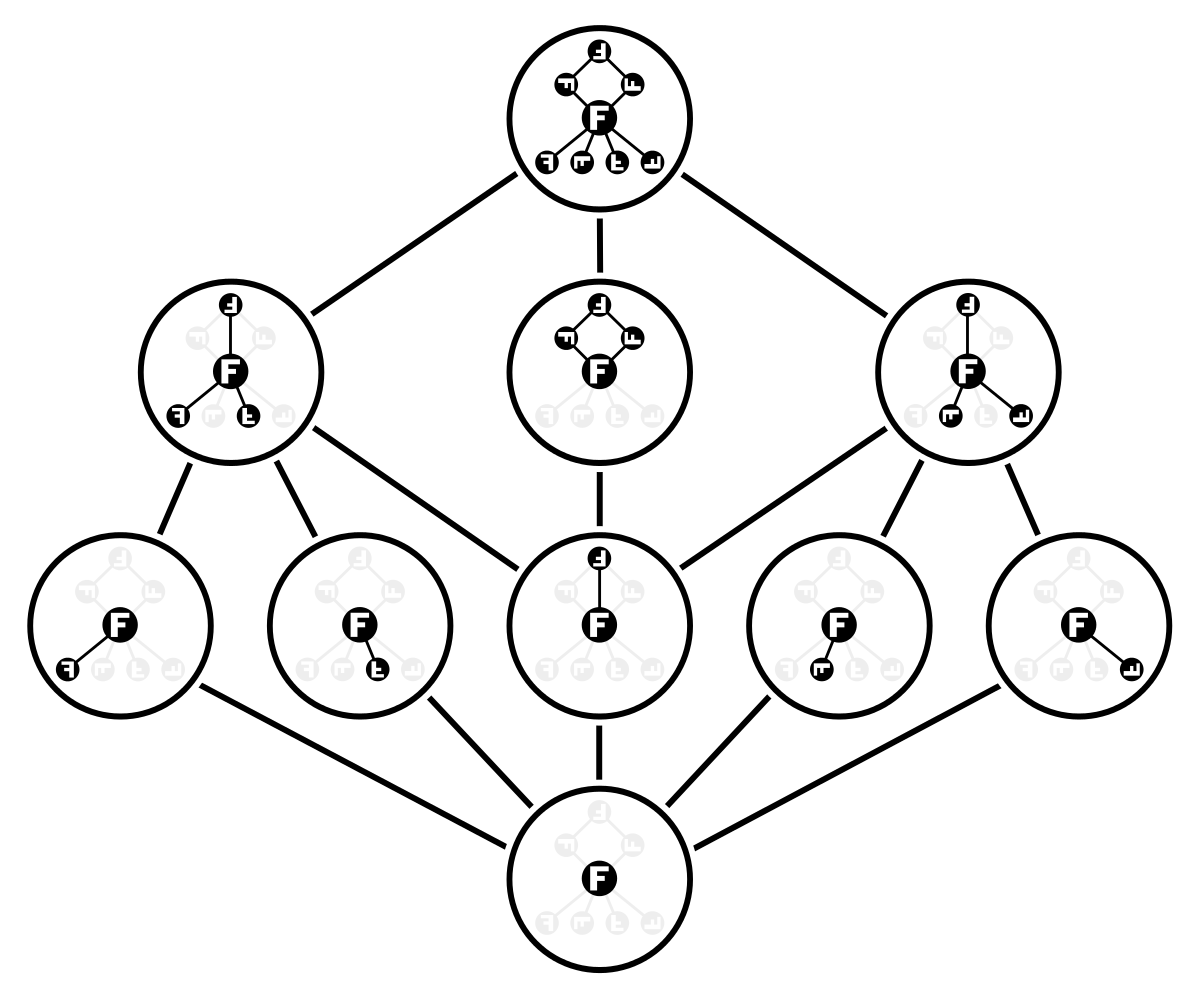
\includegraphics[width=0.75\paperwidth]{Figures/Dihedral_4_subgroup_lattice.svg.png}\transparent{1}};
\draw (current page.center) node [fill=ocre!30!white,fill opacity=0.6,text opacity=1,inner sep=1cm]{\Huge\centering\bfseries\sffamily\parbox[c][][t]{\paperwidth}{\centering Modern Algebra with Friends\\[15pt] % Book title
{\Large A Companion Note-set for ``Topics in Algebra 2nd ed." by I. N. Herstein \nocite{herstein1991topics}}\\[20pt] % Subtitle
{\huge Hall, Hall, Stephenson, Estrada, and Pauley}}}; % Author name
\end{tikzpicture}
\vfill
\endgroup

%----------------------------------------------------------------------------------------
%	COPYRIGHT PAGE
%----------------------------------------------------------------------------------------

\newpage
~\vfill
\thispagestyle{empty}

\noindent Copyright \textcopyright  \ 2023 J. J. Hall, J. S. Hall, D. T. Stephenson, P. Estrada, J. A. Pauley \steezybreak% Copyright notice

\noindent \textsc{Published by The Friendly Publishing Co.}\steezybreak % Publisher

\noindent \textsc{our-nice-website.com}\steezybreak % URL

\noindent Licensed under the Creative Commons Attribution-NonCommercial 3.0 Unported License (the ``License''). You may not use this file except in compliance with the License. You may obtain a copy of the License at \url{http://creativecommons.org/licenses/by-nc/3.0}. Unless required by applicable law or agreed to in writing, software distributed under the License is distributed on an \textsc{``as is'' basis, without warranties or conditions of any kind}, either express or implied. See the License for the specific language governing permissions and limitations under the License.\steezybreak % License information, replace this with your own license (if any)

\noindent \textit{First printing, December 10th, 2020}\\ % Printing/edition date
\noindent \textit{This version's compile date: \today}

%----------------------------------------------------------------------------------------
%	TABLE OF CONTENTS
%----------------------------------------------------------------------------------------

%\usechapterimagefalse % If you don't want to include a chapter image, use this to toggle images off - it can be enabled later with \usechapterimagetrue

\chapterimage{chapter_head_1.pdf} % Table of contents heading image

\pagestyle{empty} % Disable headers and footers for the following pages

\tableofcontents % Print the table of contents itself

\cleardoublepage % Forces the first chapter to start on an odd page so it's on the right side of the book
\setcounter{chapter}{-1}
\section{Foreword}
This text takes direct inspiration from the MATH 421 Course that was offered at Miami University in Oxford, OH in the Fall semester of 2012. This course was instructed by the co-author's professor Dr. Katherine Magurn. Dr. Magurn was gifted, unlike any other, in her ability to take dense material, that would otherwise \textit{only} be accessible to mathematicians with some prior knowledge, and make it accessible to individuals who had little or no formal background in mathematics. This course was intended to not only review the fundamental topics of Abstract Algebra, but to teach students how to \textit{generate} and \textit{verify} substantial proof of claims. The world of mathematics is a vast and varied one, but across almost every discipline in mathematics, the tools learned here can again be used to gain deep understanding about newly discovered, defined, or considered mathematical objects and structure. 

The authors' original intent for this text is to  provide: 1) an overview of the tools and techniques used to make formal arguments and proofs about particular mathematical structure(s) or objects. 2) provide a primer on topics of Modern Algebra that make topics of Category Theory far more accessible to individuals who have not pursued an undergraduate mathematics degree (because let's face it, it is no trivial task to learn Category Theory without \textit{at least} an undergraduate Math degree). If you are reading this text for the second of these purposes, might we suggest the reader consider Steven Roman's text \textit{``An Introduction to the Language of Category Theory"} after finishing this text, as many of the examples covered in Roman's text are drawn from the topics covered in this course. In his book, Roman generalizes many  concepts of Abstract Algebra, covered here, into concepts that pertain to the language of Category Theory.

This class is intended to be accessible to an undergraduate who has completed Algebra II or an eager high schooler who has done the same. We hope that this class will give you the tools required to begin study in a great variety of disciplines of higher mathematics; it will teach you many methods of proof and the fundamental tools of first-order (and second-order) logic while simultaneously teaching you the fundamentals of Modern Algebra: relations, group theory, ring theory, field theory, etc. What's more is that from this very abstract, high-level point of view, the proofs are simple and elegant. 
\noindent The authors believe that understanding this material will unlock many doors for the readers and as such we hope that you will use this newfound knowledge for the good of mankind. We are all alone here on this rock, please take care of one another.\steezybreak
\small
\begin{quote}
Abou Ben Adhem (may his tribe increase!)\\
Awoke one night from a deep dream of peace,\\
And saw, within the moonlight in his room,\\
Making it rich, and like a lily in bloom,\\
An angel writing in a book of gold:—\\
Exceeding peace had made Ben Adhem bold,\\
And to the presence in the room he said,\\
"What writest thou?"—The vision raised its head,\\
And with a look made of all sweet accord,\\
Answered, "The names of those who love the Lord."\\
"And is mine one?" said Abou. "Nay, not so,"\\
Replied the angel. Abou spoke more low,\\
But cheerly still; and said, "I pray thee, then,\\
Write me as one that loves his fellow men."\steezybreak

The angel wrote, and vanished. The next night\\
It came again with a great wakening light,\\
And showed the names whom love of God had blest,\\
And lo! Ben Adhem's name led all the rest.\steezybreak

- J. H. Leigh Hunt
\end{quote} 


\section{Acknowledgements}
The authors are so grateful to the many individuals who have helped in the writing of this text. Your careful corrections and improvements have made the text clearer and more readable for all.
 \\ \\
In particular we would like to thank Dr. Edwin K. P. Chong for his consistent constructive feedback and for his uncanny (superhuman?) talent to distill tedious arguments into the bare essentials while somehow still maintaining excellent readability! \\ \\
We would like to thank Dr. Robert Vanderwall for his corrections, constructive feedback, and valuable perspective which has extended and improved the readability of the text to a greater audience. 
\\ \\
We would like to thank Pedro Estrada for his corrections and feedback; particularly his thorough feedback for the appendix on propositional and first-order logic and the corresponding exercises. \\ \\
We would like to thank Dr. Chris Robbiano for his feedback; particularly his revisions of some of the preliminary set-theory definitions. \\ \\
\textit{Co-authors, add any acknowledgements here!} \\ \\

\noindent Lastly, we would like to thank our readers; your feedback has been invaluable in refining this text: Yifan Yang, Vladimir Yaremenko, Dr. Chris Robbiano, Dr. Robert Vanderwall, Dr. Edwin Chong, Katherine S. van der Vliet, and Ren\'{e}e Neary.
\section{Dedication}
\vspace{4in}
\begin{center}
   \textit{This book is dedicated to Dr. Katherine E. Magurn.} 
\end{center}

    


\pagestyle{fancy} % Enable headers and footers again

%----------------------------------------------------------------------------------------
%	PART
%----------------------------------------------------------------------------------------

 \part{Part One}
%----------------------------------------------------------------------------------------
%	CHAPTER 0
%----------------------------------------------------------------------------------------
\setcounter{chapter}{-1}
\nocite{*}
%--------------------
%	CHAPTER 0
%--------------------

\chapterimage{chapter_head_1.pdf} % Chapter heading image

\chapter{Preliminaries}
If you see a mistake in this document, or want further clarification somewhere, please open an issue on the book's \href{https://github.com/hilikliming/modern_algebra_with_friends}{\textul{github repository}}, or send me an email at jack.hall618@gmail.com \steezybreak \\
% \jjh{This is Jack's color}, \\
% \dts{This is Dan's color},\\
% \jsh{This is Jessie's color} \\ %% Use the command \jsh{ <insert comment here> } %% okie
% \jap{This is Jake's color}\\
% \kvdv{This is Kiki's color}
% (see lines 57-61 newcommand definitions in the main.tex for this document)\\ \\
\noindent 
\begin{tcolorbox}
    \begin{center}
\jjh{\href{https://www.dropbox.com/sh/759pwsjyc3ix0jy/AACv98R1Zpjvbaz2VhH4aH4ca?dl=0&fbclid=IwAR10ePsYI76S-MwDbBpH9fpoEbdxvyOlHs9PeaP2ZvY8SbJu1KPTxjMissA}{The Dropbox folder for this course can be found here. \\
Homework sets, a copy of this text (updated regularly), and homework solutions will be posted as we go through the material.}}\\
    \end{center}
\end{tcolorbox}


% \jjh{\href{https://youtube.com/playlist?list=PLW3u28VuDAHJNrf3JCgT0GG_rjFVz0-j9}{Another wonderful resource as you venture further into this material are Dr. Aviv Censor's lectures on Algebra (Algebra 1M Technion University). Dr. Censor covers many topics featured in this book and uses very similar conventions to our book. Thank you Dr. Censor and Technion U for making these videos public!!!}}\\
\bigbreak
\noindent Chapter 0 is meant to serve as a reference for symbols and terminology used in the main course material (Chapter 1 onward). On its own, this first Chapter is a doozy and we are going to throw all sorts of new notation at you. \textit{Don't be intimidated}. You do not need to understand or memorize all of this right away; the utility of these new notations will become apparent as you progress further through the text. Treat this chapter as a reference for the main course material that begins in Chapter 1. The authors recommend that readers who are familiar with mathematical induction already read sections 0.7 and 0.8. For readers who have never seen induction before, as to not distract from the more important intuition, we would prefer you skip 0.7 and 0.8 and read 0.8.1 first, then return to those sections after the underlying argument for the principle of induction is understood.

Lastly, when reading this material, read slowly and carefully and try to explain the argument out loud as if another were listening. Don't just read it aloud, really think about what the claim or statement is asserting. There is very little redundancy in mathematical writing so it pays dividends to read slowly, carefully, and to re-read many times until the argument is so clear that you could write it down again in your own words. When I read a new book or article in my field, the first 2-3 reads through I am just letting the new notations, jargon, definitions, and claims wash over me, I want to see the way the author uses these terms first and then I try to understand them more carefully. You can do it, you can piece it together! Just take baby steps to make your foundation solid. \newpage
\section{Common Notation seen in Herstein's book and this book}
$\blacksquare$ Denotes the end of a proof. Some authors  use the symbol \index{$\blacksquare$} $\square$\\ \\
$\exists$ read as `` There exists" \index{$\exists$} -- this symbol is commonly referred to as the ``existential quantifier"\\ \\
$\forall$ read as ``for all" \index{$\forall$} -- this symbol is commonly referred to as the ``universal quantifier"\\ \\
$\therefore \ $  read as ``therefore" \index{$\therefore$}\\ \\
$\because \ $ read as ``because" (we will use this symbol very rarely, usually we will just say "because")\\ \\
$a\in A$ read as ``$a$ is an element of $A$" or ``$a$ in $A$" \index{$\in$} \\ \\
$a\not\in A$ read as ``$a$ is \textit{not} an element of $A$" or ``$a$ not in $A$" \\ \\ \index{$\not\in$}
$\ni$ read as ``for which" or "who exhibits (\textit{pl.} exhibit ) the property..." or "who has (\textit{pl.} have ) the property..." \index{$\ni$}\\ \\

\begin{tcolorbox}
\begin{center}
NOTE: in this book \hl{$\in \neq \ni $}, i.e. "element of" and "element-wise for which" are \textit{not} the same symbol and  \underline{\hl{DO NOT mean the same thing}}.
\end{center}
\end{tcolorbox}
%or "who has (\textit{pl.} have ) the property" \\ \\ %(although some books will use $\in$ and $\ni$ interchangeably)
$| \ \ $ also read as ``for which" or "who exhibit the property..." or "who have the property..."; however this will almost always be used when referring to \textit{collections/sets} of elements "for which" a property holds (i.e. not element-wise), e.g. 
\begin{align}
    \{x\in \Z | 22\leq x < 27\}  \nonumber \\
    &= \{ \text{the subset of $\Z$ for which members are $\geq 22$ AND $<27$} \} \nonumber \\
    &= \{22,23,24,25,26\}\nonumber
\end{align}
  \\ \\%or "who has (\textit{pl.} have ) the property" \\ \\ %(although some books will use $\in$ and $\ni$ interchangeably)
$a\in A \ni P(a)$ read as `` $a$ is an element of $A$ for which Property $P(a)$ is true"\\ \\
$\implies$ read as ``implies"\\ \\
$A\implies B$ can be read as any of the following equivalent ways: ``A implies B", ``if A then B", ``A only if B" \footnote{This is important, if you need clarification look \href{https://criticalthinkeracademy.com/courses/propositional-logic/lectures/51574}{here (link)}}. We sometimes also say "$A$ is \textit{sufficient} for $B$" or "$B$ is \textit{necessary} for $A$"\\ \\ 
$\Leftrightarrow$ read as ``is equivalent to" or ``if and only if", also commonly written ``iff"\\ \\
If both ``$A$ only if $B$" is true (i.e. $A\implies B$, or, $A$ is true only if $B$ is true) and ``if $B$ then $A$" is true (i.e. $B\implies A$, or, if $B$ is true, then $A$ is true), then we say ``$A$ if and only if $B$" or "$A\iff B$" and the statements $A$ and $B$ are equivalent (see below). In this scenario we may also say "$A$ is \textit{necessary and sufficient} for $B$" or "$B$ is \textit{necessary and sufficient} for $A$" \\ \\
$A\iff B$ can also be read as ``$A$ if and only if $B$", ``$B$ if and only if $A$", ``$A$ iff $B$", ``$B$ iff $A$", ``$A$ is equivalent to $B$", ``$B$ is equivalent to $A$" lastly, this expression could also be read `` $A$ implies $B$ and $B$ implies $A$" or "$B$ implies $A$ and $A$ implies $B$". We emphasize the last two interpretations because iff statements (i.e. statements that use $\iff$) should be thought of as pairs of implications, one implication $LHS\implies RHS$ and another implication $RHS \implies LHS$. (LHS is left-hand-side here.)\\ \\
$\lnot A$ read ``not $A$" is called the negation of statement $A$ \\(e.g. $\lnot(\lnot A)\iff A$ and $x\neq y \iff \lnot(x=y)$ \ \ ) \\ \\
$\lnot B \implies \lnot A$ is called the contraposition of implication $A \implies B$. We have that $\lnot B \implies \lnot A \iff A\implies B$ (i.e. these expressions are equivalent, this is often useful for proofs, instead of proving $A\implies B$ we can prove $\lnot B \implies \lnot A$)\\ \\
The intuition for an implications equivalence with its contraposition is two parts: 
\begin{enumerate}
    \item ``If $B$ is \textit{always} true when $A$ is true ($A\implies B$), then if $B$ isn't true, $A$ must not be true ($\lnot B \implies \lnot A$)".
    \item ``If $A$ is \textit{always} false when $B$ is false ($\lnot B \implies \lnot A$), then if $A$ is true, $B$ must be true ($A\implies B$)".
\end{enumerate}
Examples of proof by contrapositive and proof by contradiction are given in the sub-sections below. \\ \\

\noindent In this text, the shorthand for ``contradiction" is a pair of arrows running into one another ``$\Rightarrow\Leftarrow$" so read this as ``contradiction".
\section{A Word About Axioms in This Book}
As of January 11th, 2021, Merriam-Webster defines the noun ``Axiom" as:
\begin{enumerate}
    \item ``a statement accepted as true as the basis for argument or inference"
    \item ``an established rule or principle or a self-evident truth".
    \item ``a maxim widely accepted on its intrinsic merit". Where, here, maxim means ``a general truth, fundamental principle, or rule of conduct".
\end{enumerate}
In the land of Mathematics, the meaning of the word ``Axiom" most closely resembles the definition given in 1. ; i.e. Axioms are statements which are assumed to be true and used as the basis for argument or inference \textit{without} justification. 

This book is not a set theory or foundations of mathematics course so we will take a \textit{few} things for granted. In this book, we will not attempt to define or construct the most fundamental tools that we begin our studies with: Sets and Integers (the set $\Z$ and properties of its elements). We will instead take these to be primitive notions that do not need justification. You can take a set to be a collection of objects, \textit{with no repeated objects}. You can also take the following facts about integers as axioms:
\noindent\begin{align}
    a,b\in \Z &\implies a+b\in \Z  \ \ \ &\text{i.e. it is always true that the sum of two integers is an integer}\nonumber \\
    \text{ and } &\implies a-b\in \Z \ \ \ &\text{i.e. it is always true that the difference of two integers is an integer}\nonumber \\
    \text{ and } &\implies \exists \ -a,-b \in \Z \ \ \ &\text{i.e. every integer has an additive opposite or "negative" that is an integer}\nonumber \\
     \text{ and } &\implies a\cdot b\in \Z \ \ \ &\text{i.e. the product of two integers is always an integer}\nonumber
\end{align} 
All of this being said, using the tools of first order logic that you will learn along the way, if you wished to, you could ``begin again" with some weaker assumptions and build your way back up to showing that e.g. adding, subtracting, or multiplying two integers gives another integer, or that every integer $a\in\Z$ has an opposite $-a\in\Z$. 

\section{Basic Set Theory Definitions}
Given a set $S$ we will consistently use the notation $A=\{a\in S\ |\ P(a)\}$ to read `` $A$ is the set of all elements in $S$ for which the property P is true". This notation is commonly referred to as \textbf{set builder} notation. We read the vertical bar `` $|$ " as ``for which" or sometimes ``such that", we will also commonly use the symbol $\ni$ to indicate ``for which" or ``such that" when we are referring to individual elements, e.g. $a\in A \ni a>0$ is read as `` $a$ is an element of $A$ for which $a>0$" or ``$a$ is an element of $A$ such that $a$ is greater than zero". \\ \\
\noindent Here is a simple example of this \textbf{set builder} notation in use, let $P(a)=$ "$a \text{ is even}$". \\
Then $\{a\in \Z | P(a)\} = \{...,-4,-2,0,2,4,6,...\} = \{ \text{the set of all even integers}\}$ \\ \\
Sometimes, in other math texts, a colon, ``$:$", will be used in place of the vertical bar, ``$|$", in set builder notation.\\ \\
\noindent We will now present five basic, but very important, definitions from Set Theory. \newpage
\begin{definition}[Subset]\index{$\subset$}
Set $A$ is a \textit{subset} of set $B$, denoted $A\subset B$, if every element of $A$ is an element of $B$, that is, if
\begin{align}
    x\in A \implies x\in B \nonumber
\end{align}
$A\subset B$ is typically read as "$A$ contained in $B$" or "$B$ contains $A$" or "$A$ is a subset of $B$"
\end{definition}
A simple visual example of $A\subset B$ can be seen in Figure \ref{fig:Subset_example}.
\begin{figure}[h!]
    \centering
    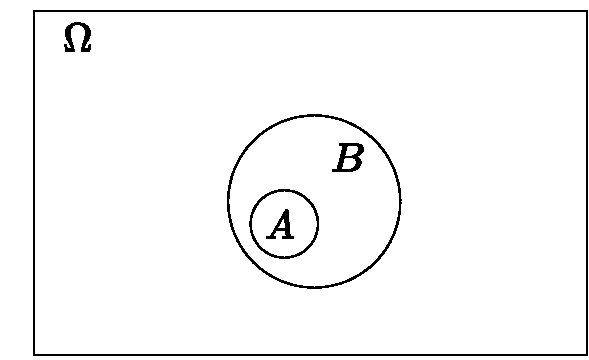
\includegraphics[width=0.5\textwidth]{Figures/SUBSET_Example.pdf}
    \caption{$A$ is a subset of $B$ since each element of $A$ is an element of $B$.}
    \label{fig:Subset_example}
\end{figure}\\
To define a set, we start with some “universe” of all possible elements of that set, usually called the \textit{universe of discourse} or simply \textit{universe}. In the figure above, our universe is denoted by $\Omega$. Then, a set $S$ can be defined by specifying which elements of the universe of discourse is in that set $S$, typically done with the set builder notation that we just introduced.
\begin{definition}[Set equality]
Sets $A$ and $B$ are equal if both $A\subset B$ and $B\subset A$
\end{definition}

\begin{definition}[Union of Sets] \index{$\cup$}
The \textit{union} of the two sets $A$ and $B$, written as $A\cup B$, is the set
\begin{align}
    A\cup B = \{x\in \Omega |x\in A \text{ or } x\in B \} \nonumber
\end{align}
\end{definition}
Let's read the above definition of $A\cup B$ in more regular speech, this equation says "A union B equals the set of elements $x$ for which $x$ is a member of A \textbf{or} $x$ is a member of B" we are using "$x$" here as a \textit{variable} and we mean that any such member $x$ who is either in $A$ \textbf{or} in $B$ (or possibly both!) is a member of this set $A$ union $B$. \\ \\
Figure \ref{fig:set_union_example} depicts a the union of two sets, $A$ and $B$.
\begin{figure}[h!]
    \centering
    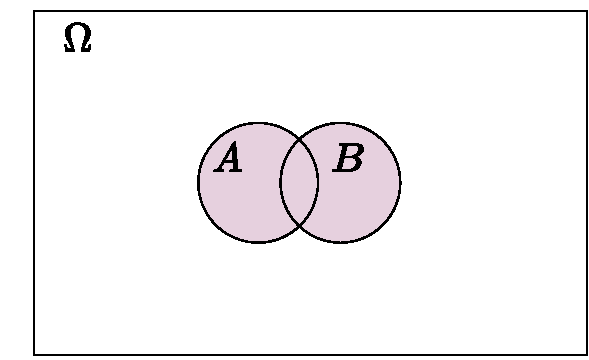
\includegraphics[width=0.5\textwidth]{Figures/Set_Union.pdf}
    \caption{The shaded region is $A\cup B$. $A\cup B$ is the set of all elements that are either in $A$ or in $B$.}
    \label{fig:set_union_example}
\end{figure}
\begin{definition}[Intersection of Sets]\index{$\cap$}
The \textit{intersection} of the two sets $A$ and $B$, written as $A\cap B$, is the set
\begin{align}
    A\cap B=\{x \in \Omega |x\in A \text{ and } x\in B \} \nonumber
\end{align}
\end{definition}
Let's read the above definition of $A\cap B$ in more regular speech, this equation says "$A$ intersect $B$ equals the set of elements $x$ for which $x$ is a member of $A$ \textbf{and} $x$ is a member of $B$". Again, we are using $x$ here as a variable and we mean that any element (who we choose to represent with the "handle" $x$) who satisfies $x$ in $A$ \textbf{and} $x$ in $B$ is a member of this set $A$ intersect $B$.\\ \\

\noindent Figure \ref{fig:set_intersection_example} depicts a the intersection of two sets $A$ and $B$.
\begin{figure}[h!]
    \centering
    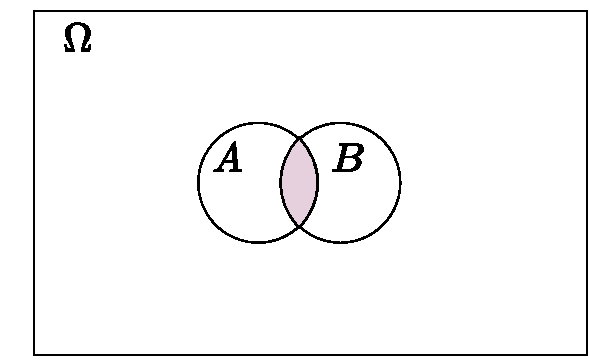
\includegraphics[width=0.5\textwidth]{Figures/Set_INTERSECTION.pdf}
    \caption{The shaded region is $A\cap B$. $A\cap B$ is the set of all elements that are both in $A$ \textit{and} in $B$.}
    \label{fig:set_intersection_example}
\end{figure}

\begin{definition}[Difference of Sets (Difference Set)]
Given two sets $A$ and $B$, then the \textit{difference set} written as $A - B$ or sometimes $A\setminus B$, is the set
\begin{align}
    A-B=\{x\in A| x\not\in B\}=\{x\in \Omega |x\in A \text{ and } x\not\in B \} \nonumber
\end{align}
\end{definition}
Note that we could define the difference set $A- B$ %lightly more generally by defining it in terms of some ``universe" set $\Omega$ who contains all the sets we are considering as subsets, i.e. $A,B \subset \Omega$. 
In another way using an idea known as set complement. In this case we would have $A- B=A\cap B^C$ where $B^C$ is referred to as the complement of set $B$ and it is defined as $B^C=\{x\in \Omega| x\not \in B\}$. For this reason, $A-B$ is sometimes called "the complement of $B$ in $A$". This form will almost never come up in this text but we mention it for interested readers who may go on to study Measure Theory (i.e. Probability), as it is an extremely convenient way to rewrite the difference of two sets when dealing with proofs in Measure Theory. 

\begin{figure}[h!]
    \centering
    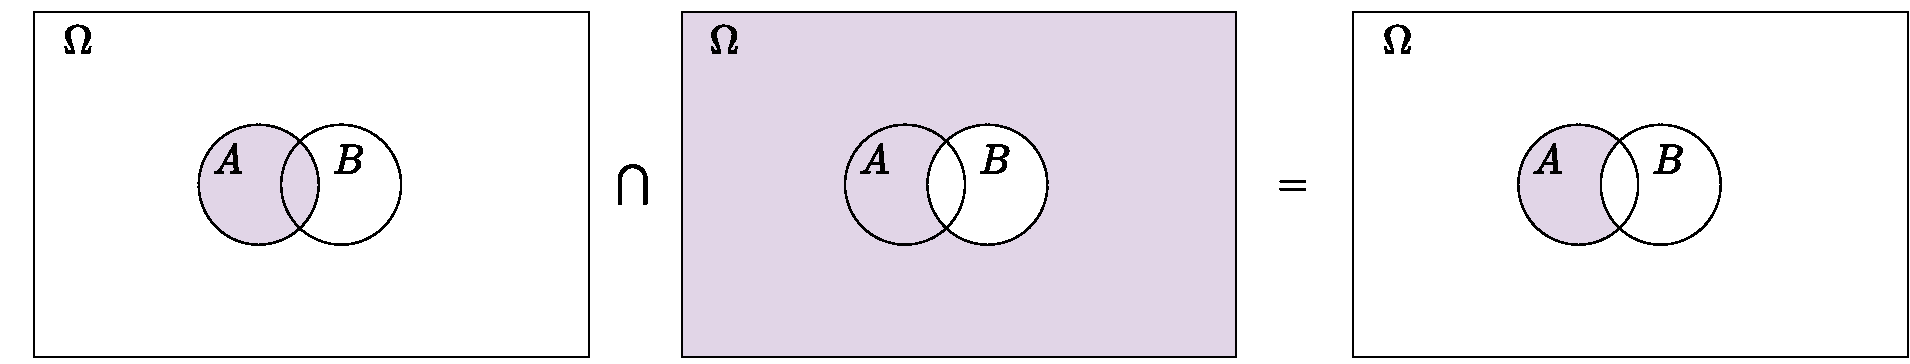
\includegraphics[width=0.9\textwidth]{Figures/Complements View of Set Minus.pdf}
    \caption{Complements View of Set Minus: on the left side of the intersection, set $A$ is shaded in, on the right side of the intersection set $B^C$ ($B$'s complement in universe $\Omega$) is shaded in, now it is easy to see that $A$'s intersection with $B^C$ (i.e. the portion these two shaded regions have in common) is simply $A-B$, or "the parts of $A$ that are not in $B$".}
    \label{fig:complements_view_set_minus}
\end{figure}
\newpage
\noindent For the two definitions provided below, the reader should note a finite union/intersection is the union/intersection of a finite number of sets; this phrase does not imply that the union/intersection set itself is a finite set!

\begin{definition}[Finite Union of Sets]
    A \textit{finite union} of sets $A_1, A_2, A_3, \dots , A_n$ could be written $A_1 \cup A_2 \cup A_3 \cup \dots \cup A_n$ (as union is associative) or, more commonly, $\bigcup_{i=1}^n A_i$. 
\begin{align}
    \bigcup_{i=1}^n A_i &= \{x\in \Omega \ | \ x\in A_1 \text{ or } x \in A_2 \text{ or } x\in A_3 \  \cdots \text{ or } x\in A_n\} \nonumber \\
    &= A_1 \cup A_2 \cup A_3 \cup \dots \cup A_n \nonumber 
\end{align}
%\textit{The second equality above can be proven using an induction argument and associativity of unions (which allows us to remove parentheses without ambiguity), some might enjoy proving this as an exercise, but it is not required. Same for the definition below and associativity of intersections}
\end{definition}

\begin{definition}[Finite Intersection of Sets]
    A \textit{finite intersection} of sets $A_1, A_2, A_3, \dots , A_n$ could be written $A_1 \cap A_2 \cap A_3 \cap \dots \cap A_n$ (as intersection is associative) or, more commonly, $\bigcap_{i=1}^n A_i$. 
\begin{align}
    \bigcap_{i=1}^n A_i &= \{x\in \Omega \ | \ x\in A_1 \text{ and } x \in A_2 \text{ and } x\in A_3 \ \cdots \text{ and } x\in A_n\} \nonumber \\
    &= A_1 \cap A_2 \cap A_3 \cap \dots \cap A_n \nonumber 
\end{align}
\end{definition}

\begin{definition}[Disjoint Sets]
    Sets $A, B$ are said to be disjoint if $A\cap B= \emptyset=\{\}$\steezybreak \\
    \noindent That is, a pair of sets are disjoint if they share no elements in common (hence, their intersection is the empty set)
\end{definition}

\noindent Figure \ref{fig:disjoint_sets} depicts an example of two sets $A$ and $B$ that are \textit{disjoint}, that is, they share no elements and their intersection is the empty set.
\begin{figure}[h!]
    \centering
    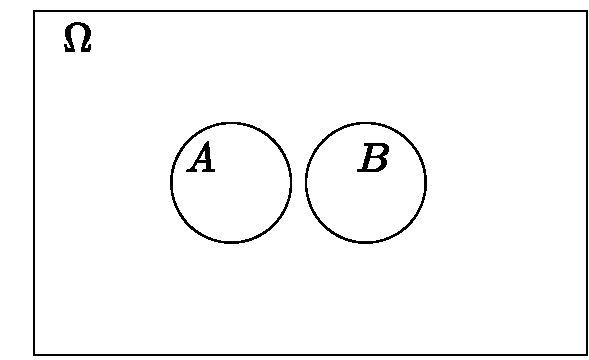
\includegraphics[width=0.5\textwidth]{Figures/disjoint_sets.pdf}
    \caption{$A$ and $B$ have no elements in common so $A\cap B=\emptyset$.}
    \label{fig:disjoint_sets}
\end{figure}

\begin{definition}[Mutually Disjoint (Collection of) Sets]
    A collection of sets $A_1,A_2,...,A_n$ are said to be mutually disjoint if $A_i\cap A_j=\emptyset$ whenever $i\neq j$ \\

    \noindent That is, a collection of sets are mutually disjoint when each set in the collection contain no common elements with any other set in the collection (aside from itself).
\end{definition}
\newpage 
\noindent\section{Some important sets to remember}
% \begin{align}
% \emptyset=\{\} =\text{ The empty set (set with no elements, $\emptyset$ is trivially a subset of all sets) } \nonumber \\
% \text{Bool}= \{T,F\} \nonumber \\
% \mathbb{Z}=\{..,-3,-2,-1,0,1,2,3,...\}= \text{ the integers} \nonumber\\
% \mathbb{Q}=\{\frac{a}{b} \ | \  a,b \in \mathbb{Z} \ni b\neq 0\}= \text{ the rationals} \nonumber\\
% \mathbb{R}=\{\ ...c_1c_0.c_{-1}c_{-2}...\  | \ c_i\in \{0,1,2,3,4,5,6,7,8,9\} \ \forall  i  \}= \text{ the reals} \nonumber\\
% \text{sets } A, B \text{ are said to be disjoint if } A\cap B= \emptyset=\{\} \nonumber
% \end{align}

$\emptyset=\{\}$ The empty set (set with no elements, $\emptyset$ is trivially a subset of all sets since for any set, empty or non-empty, you can always consider the collection of \textit{none} of its elements, this is exactly the empty set) \index{$\emptyset$} \index{$\{\}$}\\
%$\text{Bool}= \{T,F\}$ \\
% Originally decided to let 0 be in N but since we've never really needed it I'm redefining now (10/26/2023) let me know if this change is in conflict with anything I wrote later lol
$\mathbb{N}=\{1,2,3,4,...\}$  = the natural numbers\\ 
$\mathbb{Z}=\{..,-3,-2,-1,0,1,2,3,...\}=$ the integers\\
$\mathbb{Q}=\{\frac{a}{b} \ | \  a,b \in \mathbb{Z} \ni b\neq 0\}$= the rationals \\
$\mathbb{R}=\{\ ...c_1c_0.c_{-1}c_{-2}...\  | \ c_i\in \{0,1,2,3,4,5,6,7,8,9\} \ \forall  i  \}=$ the reals\\ \\
\subsection{Interval Notation for Interval Subsets in $\R$}
We will use the following standard interval notation for \textit{interval subsets} of $\R$.\\ 
Let $a,b\in \R, a<b$ we denote the following sets:\\
$(a,b)= \{r\in \R | a<r<b \} \subset \R$,\\
$[a,b)= \{r\in \R | a\leq r<b \} \subset \R$, \\ 
$(a,b]= \{r\in \R | a< r\leq b \} \subset \R$, and lastly, \\
$[a,b]= \{r\in \R | a\leq r \leq b \} \subset \R$ \\ 

\noindent A key observation about the above interval notations is that square brackets, "$[$" or "$]$", are used when a given "endpoint" (i.e. $a$ or $b$) \textit{is} a member of the subset. Round brackets, "$($" or "$)$", are used when a given "endpoint" \textit{is not} a member of the subset. From examples above this means $a\not \in (a,b]$ but $b\in (a,b]$ and similarly $a,b\in [a,b]$, but $a\not \in (a,b)$ and $b \not \in (a,b)$.\\ \\

\section{Proof by Contrapositive Example} Let $x\in \mathbb{Z}$ and suppose we have statements $A=$``$x^2$ is even" and $B=$``$x$ is even", and wish to prove $A\implies B$, we can instead prove $\lnot B \implies \lnot A$ where $\lnot B=$``$x$ is not even" and $\lnot A=$``$x^2$ is not even". This latter statement is equivalent to the former and a proof by contraposition goes as follows: suppose that $x$ is not even, then $x$ is odd. The product of two odd numbers is odd, hence $x^2 = x\cdot x$ is odd. Thus $x^2$ is not even. Having proved the contrapositive, we can then infer that the original statement is true, i.e. that $A \implies B$ \\ \\
\href{https://www.math.toronto.edu/preparing-for-calculus/3_logic/we_3_negation.html}{Click Here for help with negating logical expressions. (See table at end of webpage)}\\

\noindent This is not to be confused with proof by contradiction. In proof by contradiction we have statement $A\implies B$ that we wish to show. To accomplish this, we begin by assuming $A$ is true \textit{and} that $B$ is false and we will arrive at a contradiction (notated as $\Rightarrow\Leftarrow$) that is a direct consequence of our incorrect assumption about $B$, meaning the only possibility is that our assumption about $B$ being false when $A$ is true was incorrect, meaning that if $A$ is true then $B$ must be true too, giving us the desired result: $A \implies B$ \newpage
\noindent\section{Proof by Contradiction (a.k.a. 
\textit{Reductio ad absurdum}) Example:} In this example\footnote{ A reader who already knows some Category Theory and is fond of Type Theories may scoff at this example for Reductio ad absurdum as it relies on another (dubious?) tool (LOTEM). We will be working with Classical Logic for the time being, and under those rules, this is all fine. I may discuss introduction and elimination rules we've been using ( see Dr. Mark Jago's excellent lectures here: \textcolor{orange}{\href{https://www.youtube.com/watch?v=dlUkeN7KqVA&t=8s}{Propositional Logic/Classical Natural Deduction}/ \href{https://www.youtube.com/watch?v=C30w5vZypXE}{First-Order Logic}}) towards the end of the text and allude to logics that relax assumptions like double negation elimination. Stick with us, you may enjoy the presentation of the algebraic topics covered here \smiley } we will prove an implication using \textit{Reductio ad absurdum} or proof by contradiction. Given statements $A= "x^2 \text{ is even}"$, and $B= "x \text{ is even}"$, we could show $A\implies B$ through the following contradiction: Assume $A$ true and $\lnot B$ true, that is assume ``$x^2 \text{ is even}$" and ``$x \text{ is not even}$", now since $x$ is odd, and the product of two odds is odd, $x\cdot x$ is odd, but $x\cdot x=x^2$ and $x^2$ was assumed even! $\Rightarrow\Leftarrow$ (contradiction!). What we have shown is that $\lnot B$ cannot be true when $A$ is true. So our only option left is to conclude that if $A$ is true, then $B$ is true, i.e. $A\implies B$ %Given statements $A=$``The match is burning" and $B=$``There is oxygen in the room" we could show $A\implies B$ through the following contradiction: Assume $A$ true and $\lnot B$ true, that is assume ``The match is burning" and ``there is not oxygen in the room", immediately we arrive at a contradiction because as any person who has snuffed a candle knows ``burning " cannot occur without oxygen $\Rightarrow \Leftarrow$ (arrows running into each other is used to indicated a contradiction) therefore $\lnot B$ cannot be true when $A$ is true. So we have pigeon-holed our option for the true-ness or false-ness of statement B which statement A is assumed to be true, so our only option left is to conclude that when $A$ is true, $B$ must be true, i.e. $A\implies B$\\ \\

\section{Proof by Induction Example} Mathematical induction is a technique of proof that is essentially used to prove that a statement $P(n)$ holds for \textit{every} natural number $n = 1, 2, 3, ...$ ; that is, the overall statement is a sequence of infinitely many cases $P(1), P(2), P(3), ...$ \\
\noindent A proof by induction consists of two cases. The first, the base case (or basis), proves the statement for $n = 1$ without assuming any knowledge of other cases. The second case, the induction step, proves that if the statement holds for any given case $n\geq 1$, then it must also hold for the next case $n + 1$. These two steps establish that the statement holds for every natural number $n$. The base case does not necessarily begin with $n = 1$, but often with $n = 0$, and possibly with any fixed natural number $n = N$, establishing the truth of the statement for all natural numbers $n \geq N$. Now we will give an example of this approach of proof in order to prove the following fact about sums of natural numbers:
\begin{align}
    \sum_{k=1}^{n} k = \frac{n(n+1)}{2} \ \ \ \forall n \in \N \nonumber
\end{align}
In the proof below we will begin by establishing the result for a \textit{base case} where $n=1$. Then, in the \textit{induction step}, we will \textit{assume} that it holds for some $n\geq 1$ and we will show that assuming this $\implies$ $n+1$ also satisfies the property. The base case, together with the induction step, show that the rule is obeyed by all natural numbers $n\geq 1$ in a domino sort of effect, since $n=1$ (base) case plus the induction step implies that $n=2$ holds, then $n=2$ plus induction step implies $n=3$ holds, and so on and so forth. The principle of induction is a formal statement of this intuitive reasoning.\\
\textit{Proof:}\\
\noindent\textit{Base case:} Let $n=1$, then it is obvious that $\sum_{k=1}^1 k = 1 = \frac{1\cdot(2)}{2}=1$\\
\textit{Induction step:} Suppose for $n\geq 1$ it is true that 
\begin{align}
    \sum_{k=1}^n k&=\frac{n(n+1)}{2}\nonumber\\ 
    \implies \sum_{k=1}^{n} k + (n+1)&=\frac{n(n+1)}{2} +(n+1)\nonumber\\ 
    &=\frac{n(n+1)}{2} +\frac{2}{2}(n+1)\nonumber\\
    &=\frac{n(n+1)+2(n+1)}{2} \nonumber \\
    &=\frac{(n+1)(n+2)}{2} \nonumber \\
    &=\frac{(n+1)((n+1)+1)}{2} \nonumber
\end{align}
Since $\sum_{k=1}^{n} k + (n+1)=\sum_{k=1}^{n+1} k$ we have shown that arbitrary $n\geq 1$ obeying the rule \textit{implies} that $n+1$ also obeys the rule. This induction step, along with the base case for $n=1$ completes the proof. $\blacksquare$
\smallbreak

\section{A common pitfall when first learning Proof by Induction}
%\noindent Having just covered the principle of mathematical induction, the authors want to emphasize that both of the steps used (i.e. the base case, and inductive step) play an \textit{equal role} in proof of the fact. We emphasize the importance of the \textit{base case} first and then will use an example to show how base case oversights can often reveal themselves in the inductive step. In particular, we emphasize that when choosing the base case, the proof-writer should ensure that the base case is satisfied because of a property that follows from the assumptions about the claim, and not from a property of the \textit{specific} base case that was chosen. \\

%\noindent When choosing the base case above you might notice that we chose $n=1$ instead of $n=0$, partly this is because the claim only pertained to $n>0$, but the other reason for this is because while, $n=0$ satisfies the rule, (i.e. $0(0+1)/2=0$, it satisfies the rule in a trivial way, because the $0$ on the left annihilates the $1/2$ on the right and the sum of $0$ numbers $k$ is itself 0. \\ \\
%\noindent To make this more clear, what if you wanted to prove the obviously false statement that for $n>0, n^3\leq n^2$. \\ \\
%\textit{Bad Base case:}\\
%If we chose $n=1$ to be our base case, we can see that we (\textit{trivially}) satisfy the claim since $1^3=1\leq 1^2 = 1$, if we continued in this way and go on attempting to show the induction step, we may even be able to obtain an (erroneous) proof of this (false) statement. This proof has begun erroneously because the base case was chosen without care. It satisfied the statement about natural numbers, not because it was a natural number who is greater than 0, but because it was the \textit{specific} natural number $1$ (who has the property that all of his powers are the same, $1$).\\

\noindent Let's have a look at another induction proof and  see how a sneaky oversight is made in the proof of the inductive step. The reader should note that \textit{up until} this oversight is made, the proof is valid. That is, this oversight, is the \textit{sole} reason this proof is false. \\ \\
\noindent \textit{False theorem:} All horses are the same color.\\ \\
\textit{An Erroneous Proof by induction:}\\ \\
$P(n)$ is the statement: In every set of horses of size $n>0$, all $n$ horses are the same color.\\ \\
\textit{Base Case or $P(1)$}: One horse is the same color as itself. This is true by inspection. \\
\textit{Induction Step}: Assume $P(n)$ for some $n\geq 1$. Since $\{H_1,...,H_n\}$ is a set of $n$ horses, the induction hypothesis applies to this set. Thus, all the horses in this set are the same color.
Since $\{ H_2,...,H_{n+1}\}$ is also a set of $n$ horses, the induction step likewise holds for this set. Thus, all the horses in this set are the same color too. Lastly we note that these sets have horse $H_2$ in common, therefore, all $n+1$ horses in $\{H_1,...,H_n,H_{n+1}\}$ are the same color. $\blacksquare$

%This proof can be thought of as being erroneous for 2 reasons and in some ways these reasons are tied to each other as the reader will see. 
%The first reason this proof is erroneous is because the base case was again chosen without care. It satisfied the statement about collections of horses trivially, because there was only one horse, i.e. in the same way that all things are the same color as themselves, not because it was a collection of $n>0$ horses. In fact, because of the specific base case that we chose, we sneakily manage to \textit{avoid considering} the overlap of two distinct horses $H_1$ and $H_2$ because such a case does not exist for a collection containing only one horse, we only need to confirm that our one horse is the same color as the other horses but there are no "other horses". If we had instead chosen a base case of $n=2$ we would have immediately seen that this statement is not true in general since $\{\text{A Black Stallion}, \text{A White Stallion}\}$ is a collection of $2$ horses that does not satisfy the statement. \\ \\
%The explanation in the above paragraph is a very typical explanation for how choosing a poor representative for the base case can lead to a nonsensical proof. 
So it appears all horses are the same color? Well, there is a mistake in this proof. Can you see what assumption was made without justification?\\ \\
In the last sentence of the \textit{induction step}, we said ``lastly, we note these sets have horse $H_2$ in common." This statement is not necessarily true, is it? Because $H_2 \in \{H_1,...,H_n\}$ is true if and only if $n\geq 2$! The only way we could be sure $H_2 \in \{H_1,...,H_n\}$ is if $n\geq 2$ but we only assumed our $n\geq 1$, meaning $n$ could equal $1$ and then all bets are off about $H_2$ belonging to set $\{H_1,...,H_n\}$. If we take another tack, by instead trying to let our base case be $n=2$ and then make the induction for $n\geq 2$, we would immediately run into a problem. The problem we would encounter is that there are plenty of counter-examples which show the property does not hold for $n=2$ (e.g. $\{\text{A White Stallion},\text{A Black Stallion}\}$ is a collection of $2$ horses that does not satisfy the statement.) so we would be unable to prove our base case. Since we can find even \textit{one} counter-example, it must not be true for \textit{all} sets of horses of size $n$. \\

\noindent Whenever you are asked to prove or disprove a conjecture or claim, if you don't have a feeling about whether the conjecture is right or wrong (true or false) then you should start with some examples.  Either you will find a counter-example (disproving the claim) or you'll start to convince yourself that it's true.  Once you start to believe a conjecture and see a pattern then you can start to try to formulate a proof.  If you find that your proof isn't really coming together, then you can start to ask where it fails which, again, might lead you to a counter-example.
% The heart of our misunderstanding has now been laid bare and we can see that even having somewhat carelessly chosen the base case, it \textit{was} still true that the sets $\{H_1\}$ and $\{H_2\}$ are both collections of $n\geq 1$ horses and in each of those "collection" the horses are all the same color. Our mistake was assuming that the first of these sets should have any more than just $H_1$ which we cannot be sure of (since $n$ could be $1$) since we assumed $n\geq 1$ after making our base step.\\
%The moral of the story is that we must take care when choosing both the base case and making the induction step and we must not assume things before we have shown them!\\ \\

%(If you want even more explaining read my comment in the Ch0\_IntroTopics.tex below this sentence)\\ \\

\subsection{Induction in Fewer Words (Taken from Chong/\.Zak An Intro to Optimization 4 ed.)}
The principle of mathematical induction may be stated as follows. \\ \\
Assume that a given property of positive integers, $P(\cdot)$, satisfies the following conditions:
\begin{itemize}
    \item The number 1 possesses this property.
    \item If the number $n$ possesses this property, then the number $n + 1$ possesses it too.
\end{itemize}
The principle of induction states that under these assumptions any positive integer possesses the
property.\\

The principle of induction is easily understood using the following intuitive argument. If the number
$1$ possesses the given property, then the second condition implies that the number $2$ possesses the
property. But, then again, the second condition implies that the number $3$ possesses this property, and so on. The principle of induction is a formal statement of this intuitive reasoning.
\newpage
\section{Negating Logical Expressions}
This table provides a resource for negating the most common types of expressions that we will encounter in this class:
\begin{center}
  \begin{tabular}{|c|c|}\hline
     \textbf{Statement: $S$} & \textbf{Negation of Statement: $\lnot S$}   \\ \hline
     $A$ or $B$ & $\lnot A$ and $\lnot B$  \\ \hline 
     $A$ and $B$ & $\lnot A$ or $\lnot B$  \\ \hline
     if $A$ then $B$ & $A$ and $\lnot B$  \\ \hline
     $\forall \ x, \ P(x)$ & $\exists \ x \ni \lnot P(x)$  \\ \hline
     $\exists \ x \ni \ P(x)$ & $\forall \ x, \lnot P(x)$  \\ \hline
\end{tabular}  
\end{center}

%% EVEN MORE EXPLAINING %%
% There are many work-arounds to see that this Theorem is obviously false. Two of these approaches include: 

% 1) redefine a ``set" of ``horses" to always have $n\geq 2$ horses (i.e. a set with a single horse is not a set of horses, it is set containing a single horse) this is sort of a semantically nit-picking approach because it exposes that part of our problem was thinking that a set of "horses" could have only 1 horse to begin with. However this approach doesn't generalize very well because sometimes we \textit{do} want to let a "set" of "horses" include sets with only 1 horse.  This approach is kind of OVERKILL and forces us to rephrase the statement used to show the theorem entirely... (there is nothing wrong with this statement intrinsically... we just need to be careful about what implications we draw from from such a statement when we began by considering a collection with only 1 horse.)

% The other alternative is: 

% 2) \textit{Recognize} that while in the case with one horse, this property is satisfied, for \textit{all} other cases it is not. Then since we want to show for $n>0$ we can show $n=1$ directly as we did but we will NOT treat this as our base case for the induction (We just have to cover $n=1$ case if we are going to make our base case $n=2$ since we wanted to show it holds for $n>0$ ). Having recognized this issue, and having taken care of the earlier numbers below (i.e. $n=1$) the \textit{non-trivial} base case ($n=2$), we will instead set the base case to be $n=2$ and the false-ness of the claimed theorem is immediately apparent as this base has many immediate counter examples to the statement such as the set listed above with different colored stallions. This second approach is almost always the way to go because in induction proofs we are showing an infinite cascade of things are true ($\forall n \in \N, P(n)$), so all you need is one counter example to show the whole thing isn't true ($\exists n\in \N \ni \lnot P(n)$). \\ \\


%\noindent Reading this should be somewhat alarming to the reader and hopefully highlights the importance of choosing a base case that does not \textit{trivially} (i.e. for a reason other than the assumed property, such as the special properties that 1, 0 have in the set of natural numbers, or the special ``pigeonholing" that occurs when we consider 1 horse's similarity to "all other horses" in a set of 1 horses that it belongs to itself!) satisfy the claim we wish to show in induction proofs.




%----------------------------------------------------------------------------------------
%	CHAPTER 1
%----------------------------------------------------------------------------------------

%----------------------
%	CHAPTER 1
%----------------------

\chapterimage{chapter_head_2.pdf} % Chapter heading image

\chapter{\texorpdfstring{Relations, Mappings, and $\Z$}{Relations, Mappings, and Z (integers)}}
\vspace{-0.1in}
\section{Relations and Equivalence Relations}
\begin{definition}[Relations]
A \textit{relation}\footnote{
    A relation \textit{between} sets $A$ and $B$ is a subset $R\subset A\times B$ with $(a,b)\in R \iff a\sim b $. If $A=B$ the relation is called ``homogeneous" and we commonly say relation ``on" $A$ as above, if $A\neq B$ the relation is called ``heterogeneous"
} on a set $A$ is a statement in two variables which is either true or false for values in $A$
\end{definition}
\begin{example}
$A=\{\text{people in this room}\}$\\
$x\sim y \Leftrightarrow x \text{ was born in the same month as } y$\\
Read the above expression as ``$x$ is related to $y$ if and only if (iff) $x$ was born in the same month as $y$"
\end{example}
\begin{example}
$A=\mathbb{R}$\\
$x\sim y \Leftrightarrow x \geq y$\\
so if we think of $\sqrt{2}$ and $0$ we have that $\sqrt{2}\geq 0$ so $\sqrt{2}\sim 0$, \\
However, since $0 \not\geq \sqrt{2} \Rightarrow 0\not\sim \sqrt{2}$
\end{example}
\begin{definition}[Reflexive, Symmetric, and Transitive Relations]
The relation $\sim$ on a set $A$ is said to be:
\begin{enumerate}[label=\roman*)]
    \item \textit{Reflexive} iff $x\sim x \ \forall x \in A$
    \item \textit{Symmetric} iff $x\sim y \Rightarrow y\sim x \ \forall \ x,y \in A$
    \item \textit{Transitive} iff $x\sim y$ and $y\sim z \Rightarrow x\sim z \ \forall x,y,z \in A$
\end{enumerate}
\end{definition}
A relation need not have any of these properties but if \textit{all three} of these properties hold, then $\sim$ is an \textit{equivalence relation} but that's important enough to get its own definition:
\begin{definition}[Equivalence Relation]
A relation $\sim$ on a set $A$ is an \textit{equivalence relation} if all three of the following hold:
\begin{enumerate}[label=\roman*)]
    \item Relation $\sim$ on $A$ is reflexive.
    \item Relation $\sim$ on $A$ is symmetric.
    \item Relation $\sim$ on $A$ is transitive.
\end{enumerate}
\end{definition}
Note that Example 1 is an equivalence relation, but Example 2 is not because it is not symmetric.
\newpage
\begin{example}
The relation ``equals" (``=") is an equivalence relation on $\mathbb{R}, \mathbb{Q}, \mathbb{Z}$ (i.e. on reals, rationals and integers). In fact, an equivalence relation is a generalization of equality, measuring equality up to some property.
\end{example}
% \noindent\textbf{Example 3:} The relation ``equals" (``=") is an equivalence relation on $\mathbb{R}, \mathbb{Q}, \mathbb{Z}$ (i.e. on reals, rationals and integers) \steezybreak\\
\begin{definition}[Even]
$n\in \mathbb{Z}$ is \textit{even} iff $n$ is an integer multiple of $2$ \\
that is, \\
$n\in \mathbb{Z} \text{ is}\textit{ even }\Leftrightarrow \exists \ k \in \mathbb{Z}$ such that $n=2k$
\end{definition}
%\noindent\textbf{Defn:} $n\in \mathbb{Z}$ is ``even" iff $n$ is an integer multiple of $2$ \\
%$\Leftrightarrow \exists k \in \mathbb{Z}$ such that $n=2k$\steezybreak\\

\begin{example}
Prove that $\sim$ is an equivalence relation on $\mathbb{Z}$:\\
$x\sim y \iff x-y \text{ is even}$\steezybreak\\

\noindent\textbf{Proof:} To prove we must show $\sim$ is reflexive, symmetric, and transitive on $\mathbb{Z}$.\\
\textit{Reflexivity:} Take $x\in \mathbb{Z}$, then $x-x=0=2*0$, since $0\in \mathbb{Z}$, $x-x$ is even. $\implies x\sim x \ \forall x \in \mathbb{Z}$\\
\textit{Symmetry:} Assume $x\sim y$, then $x-y$ is even which means $\exists k \in \mathbb{Z}$ such that $x-y=2k$. From here we can see $y-x=-(x-y)=-2k=2(-k)$, since $k\in \mathbb{Z}$, $-k\in \mathbb{Z}$ so $y-x$ is even too so we have $y\sim x$\\
\textit{Transitivity:} Assume $x\sim y$ and $y \sim z$. These expression imply the existence of two integers. The first expression implies $\exists \ k\in \mathbb{Z}$ such that $x-y=2k$ and the second expression implies $\exists \ l \in \mathbb{Z}$ such that $y-z=2l$. Using these we can see that $x-z=x-y+y-z=2k+2l=2*(k+l)$ since $k+l$ is a sum of integers, it is itself an integer so $x-z$ is even which implies $x\sim z$. So we have shown that assuming $x\sim y \text{ and } y\sim z \implies x\sim z \ \forall x,y,z \in \mathbb{Z}$. $\ \ \ \blacksquare$
\end{example}
\subsection{Understanding the First Proof}
Since this was the first proof in the course material we would like to take a few paragraphs to unpack the reasoning in the proof above. \steezybreak\\
\noindent We are asked to show that the relation defined in example 1.1.4 ($x\sim y \iff x-y \text{ is even}$) on $\Z$ is an equivalence relation. To do this we are required to show the defined relation exhibits three properties: reflexivity, symmetry, transitivity. We started by showing $\sim$ on $\Z$ has the reflexivity property. If we re-read the definition of reflexivity we see this property is a statement that pertains to \textit{every} element $a\in A$ for a relation that is defined on set $A$ (in this example $A=\Z$), it says that $\sim$ is reflexive on $A$ iff it is true that $a$ is related to itself for all $a\in A$. The reader may now be re-reading the proof and asking themselves ``So to prove $\sim$ is reflexive on $A$, don't we have to prove the reflexive property (i.e. $a\sim a$) holds for \textit{all} of the $a's$ in $A$? It looks like we only considered one?" This brings us to a very important point! \steezybreak\\

\noindent The first of these questions is certainly valid, and yes, we \textit{do} need to show this property holds for \textit{all} of the $x\in \Z$. However, the second question is a little misleading. We did consider a single $x\in \Z$, but this $x$ was \textit{arbitrary}, we did not pick $1$, or $2$ or $-664$, we instead chose "$x$", a \textit{variable}, to represent an arbitrary member of the set $\Z$ and then we \underline{only} made statements and inferences about $x$ that are true for \textbf{every} member of $\Z$ (i.e. we never used special properties of a specific member who $x$ could have been, such as $1$ or $2$, all we knew about $x$ is that it is an integer, and by being an integer it inherited any properties that are true for all integers). As a result, statements and inferences that were made about $x$ apply to \textit{all} members of the set $\Z$. \steezybreak\\
With this in mind let's break down each of the sentences in this proof starting with the reflexivity line. We first say ``Take $x\in\Z$, then $x-x=0$", we begin by considering an arbitrary representative of the set (that we call ``$x$" providing us a handle, so to speak, for "an arbitrary element of $\Z$") on which the relation is defined. We then note that for ANY element in $\Z$ it's true that $x-x=0$. Then we have another equality that says $=2*0$, this equality is pointing out that $x-x$ is an integer multiple of $2$, the integer is $0$. From here we simply look back at the definition of "even" and we see that $x-x$ is even. Then since the defined relation is an $\iff$ (i.e. a pair of implications) this means that $x\sim x \implies x-x \text{ is even}$ (we don't use this direction) AND it means that $x-x \text{ is even}\implies x\sim x$ (we use this direction). Using the latter of these implications, since we showed that $x-x$ is even, this implies that $x\sim x$, lastly, since our $x$ was chosen arbitrarily we have shown the property holds for all of the possible members of $\Z$. Hopefully, this clarifies proof of the reflexivity portion.\steezybreak\\
Next we will discuss the part of the proof that pertained to showing the symmetry property. Let's look back at the definition of a symmetric relation. In Defn 1.1.2 we say that relation $\sim$ on set $A$ is symmetric iff $x\sim y \implies y\sim x \ \forall \ x,y \in A$. In more plain speech this says a relation is symmetric iff \textit{whenever} it is true that $x\sim y$ this \textit{implies} it is also true that $y\sim x$. So to show symmetry, we must first assume that there is a related pair $x,y$ in $A$ for which $x\sim y$ that \textit{could} exist, and we show \textit{if such a pair exists} then it implies that $y\sim x$.

We begin by assuming there are some $x,y\in \Z$ with $x\sim y$ because symmetry is a property concerned with related pairs, we don't \textit{need} to consider an arbitrary $x\not\sim y$ because all we want to show is that: \textit{if there were} some pair where $x\sim y$ is true \textit{then} $y\sim x$ must also be true. \steezybreak\\
Let's break this symmetry part down. We first say ``Assume $x\sim y$, then $x-y$ is even", We begin by assuming there could be some related pair $x\sim y$ and we want to show if such a related pair exists then it is also true that $y\sim x$. We infer that $x-y$ is even because the assumption said $x\sim y$ and the definition of $\sim$ for this example tells us that $x\sim y \implies x-y \text{ is even}$. Then we say ``which means $\exists \ k\in \Z$ such that $x-y=2k$" This is just applying the definition of "even" after we confirmed that $x-y$ must be even. Lastly we say `` From here we can see $y-x=-(x-y)=-2k=2(-k)$, since $k\in \Z$, $-k\in \Z$ so $y-x$ is even too and we have $y\sim x$". So after having established that $x-y$ is even, we take a look at what $y-x$ is and realize that $x-y$ even \textit{implies} $y-x$ even since every integer $k\in \Z$ has an additive opposite $-k\in \Z$. Since we considered an arbitrary related pair (i.e. arbitrary $x,y\in \Z$ for which $x\sim y$) and we showed that just based on the fact that $x,y$ were integers and the way the equivalence relation is defined, this implies that $y\sim x$ must be true too.\steezybreak\\
Lastly, we will discuss the reasoning for the transitive step of the proof. In a similar fashion to the symmetric proof, in order to show a relation $\sim$ is \textit{transitive} we must consider an arbitrary triple $x,y,z \in \Z$ for which $x\sim y$ and $y\sim z$ and we must show that assuming $x\sim y$ and $y\sim z$ \textit{implies} that $x\sim z$.\steezybreak\\
We begin by assuming an arbitrary pair of relations $x\sim y$ and $y\sim z$ are true and we want to show that with the way $\sim$ is defined, it implies that $x$ must be related to $z$. We say ``These expressions imply the existence of two integers", this is because $x\sim y\implies x-y \text{ even }\implies \exists \ k\in \Z \ni x-y=2k$ AND $y\sim z\implies y-z \text{ even}\implies \exists \ l\in \Z \ni y-z=2l$. Next we realize that $x-z$ can be rewritten as the sum of $x-y$ and $y-z$ (both of whom are even) and we see that $x-z$ must too be even, then by the definition of the relation $x-z \text{ even}\implies x\sim z$. Again, since we showed this for an arbitrary triple $x,y,z\in \Z$ for which $x\sim y$ and $y\sim z$ using only properties that were assumed true for the argument (i.e. $x\sim y$ and $y\sim z$) or that are true for all integers, it is true for all triples $x,y,z\in \Z$ for which $x\sim y$ and $y\sim z$.


\subsection{Equivalence Classes}
\begin{definition}[Equivalence Class]
Given an equivalence relation $\sim$  on $A$ and $a\in A$, the \textit{equivalence class} of $a$ is defined as follows:
\begin{equation}
    cl(a)=\{x\in A | x \sim a\} \nonumber
\end{equation}
That is, the equivalence class of $a$, $cl(a)$, is the subset of elements in $A$ who are related to $a$.
\end{definition}
% \noindent\textbf{Defn:} Given $\sim$ an equivalence relation on $A$ and $a\in A$, the equivalence class of $a$ is defined as follows: \steezybreak\\
% $cl(a)=\{x\in A | x \sim a\}$\steezybreak\\
\noindent Looking back at the equivalence relation $\sim$ defined in example 1.1.4 on $\Z$, what's $cl(0)$?\\
\begin{align}
    cl(0)&= \{x\in \mathbb{Z}| x\sim 0\} \nonumber\\
    &= \{x\in \mathbb{Z}| x-0 \text{ is even}\}\nonumber\\
    &= \{x\in \mathbb{Z}| x \text{ is even}\}\nonumber\\
    &= \{...,-4,-2,0,2,4,6, ...\}\nonumber
\end{align}
Similarly,
\begin{align}
    cl(1)&= \{x\in \mathbb{Z}| x\sim 1\} \nonumber\\
    &= \{x\in \mathbb{Z}| x-1 \text{ is even}\}\nonumber\\
    &= \{x\in \mathbb{Z}| x \text{ is an even integer + 1}\}\nonumber\\
    &= \{...,-3,-1,1,3,5,7, ...\}\nonumber
\end{align} \\
\newpage
\begin{definition}[Partition]
Let $A_1, A_2, \cdots , A_n$ be subsets of set $A$. Subsets $A_1, A_2, ..., A_n$ \textit{partition} $A$ if the following two properties hold:
\begin{enumerate}[label=(\roman*)]
    \item $\bigcup_{i=1}^n A_i=A$ (union gives $A$)
    \item $A_i\cap A_j = \emptyset \ \ \ \forall\  i\neq j, \ i\leq j, \ j\leq n$ (subsets are mutually disjoint)
\end{enumerate}
\end{definition}
% \noindent\textbf{Defn:} Subsets $A_1, A_2, ..., A_n$ \textit{partition} $A$ if the following two properties hold:
% \begin{enumerate}[(i)]
%     \item $\bigcup_{i=1}^n A_i=A$ (union gives $A$)
%     \item $A_i\cap A_j = \emptyset \ \ \ \forall\  i\neq j, \ i\leq j, \ j\leq n$ (subsets are mutually disjoint)
% \end{enumerate}\steezybreak\\
\begin{theorem}[Fundamental Theorem of Equivalence Relations]                           \hspace{0.4in}
\begin{enumerate}
    \item The equivalence classes of an equivalence relation $\sim$ on $A$ partition $A$.
    \item Any partition of $A$ gives rise to an equivalence relation $\sim$ on $A$
\end{enumerate}
\steezybreak
\textit{Proof of (1):} Assume $\sim$ is an equivalence relation on $A$ with classes $A_1,A_2,...A_n$. First, we will show $\bigcup_{i=1}^n A_i=A$, to prove two sets $S,T$ are equal we must show $S\subset T$ and $T\subset S$.\steezybreak\\
take $a\in \bigcup_{i=1}^n A_i$, then $a$ is in some $A_i$ and $A_i\subset A$ by definition of equivalence classes, $\implies a \in A$ since $a$ was chosen arbitrarily we have shown $\bigcup_{i=1}^n A_i \subset A$. Now to show the other containment:\steezybreak\\
take $a\in A$, reflexivity says that $a\sim a$ therefore $a\in cl(a)$ and so $a\in \bigcup_{i=1}^n A_i$, so $A\subset \bigcup_{i=1}^n A_i$.\steezybreak\\

Next we must show that different classes are disjoint. Take any two classes $cl(a)=A_i$ and $cl(b)=A_j$. Suppose $x\in A_i\cap A_j$ (we will show that assuming this intersection has even 1 element implies $A_i$ and $A_j$  are the same sets, meaning  when you pick any two equivalence classes $A_i$ and $A_j$ either $A_i$ and $A_j$ are the same equivalence class or they share no elements).
\begin{align}
    x\in A_i &\implies x\in cl(a) \implies x\sim a \implies a\sim x \ (\text{by symmetry of} \sim) \nonumber\\
    x\in A_j &\implies x\in cl(b) \implies x\sim b \implies a\sim b \ (\text{by transitivity of} \sim) \nonumber
\end{align}
so $a\in cl(b)$. By transitivity, any other element related to $a$ is in $cl(b)$ so $cl(a)\subset cl(b)$. In a similar manner we can show $cl(b)\subset cl(a) \ \implies cl(a)=cl(b)$ meaning $A_i=A_j$. So equivalence classes are either disjoint or they are identical (i.e. if they share even a single element $a$, they are necessarily the exact same classes/subsets). This completes the proof of the first fact (1) in Thm 1.1.1 \steezybreak \\

\noindent\textit{Proof of (2):} Assume $A$ is paritioned by subsets $S_1,S_2,...,S_n$. Define the relation $\sim$ on $A: \forall x,y \in A, x\sim y \iff x$ and $y$ are in the same $S_i$. Then $\sim$ is an equivalence relation on $A$ (prove this as an exercise) and $\forall a \in A, cl(a)=$The $S_i$ in which $a$ sits.
$\blacksquare$
\end{theorem}



\section{Mappings} Let $S,T$ represent some sets.\\
\begin{definition}[Mapping (Function)]
$\sigma$ is a \textit{mapping} from $S$ (domain/source set) to $T$ (co-domain/target set), denoted $\sigma: S \rightarrow T$ if $\sigma$ associates $\forall \ s \in S$ one and only one element $\sigma(s)\in T$
\end{definition}
\noindent We call $\sigma(s)$ the \textit{image} of $s$ under $\sigma$.\steezybreak\\ 

\begin{figure}[ht!]
    \centering
    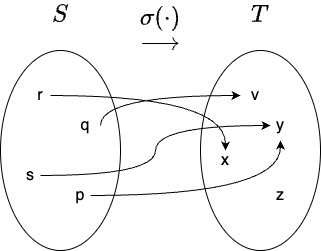
\includegraphics[width=0.45\textwidth]{Figures/Mappings_example.png}
    \caption{Mapping Example, arrows show how $\sigma$ operates on individual elements of $S$}
    \label{fig:simple_mapping_example}
\end{figure}

\begin{definition}[Image (of a set under a mapping)]
We may denote the \textit{image} of set $S$ under $\sigma$:
\begin{align}
    \text{The image of } S = \text{im} S= \{\sigma(s)|s\in S\}\nonumber
\end{align}
\end{definition} 
\begin{definition}[Pre-image (under a mapping)]
Element $s\in S$ is called a \textit{pre-image} of $t\in T$ if $\sigma(s)=t$
\end{definition}
%\noindent\textbf{Defn:} Element $s\in S$ is called a \textit{pre-image} of $t\in T$ if $\sigma(s)=t$\steezybreak\\
\begin{definition}[Inverse Image (of an element under a mapping)]
The \textit{inverse image} of $t$, denoted $\sigma^{-1}(t)$ is the set of all pre-images of $t$:
\begin{align}
    \sigma^{-1}(t)=\{s\in S | \sigma(s)=t \}\nonumber
\end{align}
\end{definition}
% \noindent\textbf{Defn:} The \textit{inverse image} of $t$, denoted $\sigma^{-1}(t)$ is the set of all pre-images of $t$:
% \begin{align}
%     \sigma^{-1}(t)=\{s\in S | \sigma(s)=t \}
% \end{align}
e.g. in Figure \ref{fig:simple_mapping_example} we have $\sigma^{-1}(x)=\{r\}$ and $\sigma^{-1}(y)=\{p,s\}$\steezybreak\\
Notice that a mapping is a special kind of relation, an equivalent definition for a mapping is as follows: A mapping from $S$ to $T$ is a subset $R\subset S \times T$ who has the property that $\forall s \in S, \exists \ \text{one and only one } t\in T \ni (s,t)\in R$, meaning that all members of the source set have a "representative" in the subset $R$, and that representative is paired with one and only one image $t\in T$. This view considers functions like lookup tables where the first entry of a given pair $(s,t)$ indicates the source element and the second entry represents the element he gets mapped to in $T$. The mapping in Figure \ref{fig:simple_mapping_example} could be written like so: $R=\{(r,x),(q,v),(s,y),(p,y)\} \subset S\times T$. When using this view, the subset of pairs, $R$, is referred to as the \textit{graph} of the mapping or function. 
\begin{notation}
When denoting mappings, Herstein prefers the notation $s\sigma$ rather than $\sigma(s)$ but the notations are related as follows: $\sigma(s) = s\sigma$, another example $\tau(a)=a\tau$, etc. 
\end{notation}

\noindent We will now present three important types of mappings.

\begin{definition}[Surjective, Injective, and Bijective Mappings]
\label{def:surj_inj_bij}
A mapping $\sigma: S\rightarrow T$ is \textit{surjective (a.k.a. onto)} if $\forall t\in T \ \exists \ s\in S \ni \sigma(s)=t$. (So $\sigma$ is surjective if every $t\in T$ has a pre-image)\steezybreak\\
A mapping $\sigma: S\rightarrow T$ is \textit{injective (a.k.a. one-to-one)} if $s_1\neq s_2 \implies \sigma(s_1)\neq \sigma(s_2)$. \\(So $\sigma$ is injective if distinct elements in $S$ \textit{stay} distinct when $\sigma$ is applied)\steezybreak\\
A mapping $\sigma: S\rightarrow T$ is \textit{bijective (a.k.a. a one-to-one correspondence)} if $\sigma$ is both injective \textit{and} surjective.
\end{definition}
% \noindent\textbf{Defn:} A mapping $\sigma: S\rightarrow T$ is \textit{surjective (a.k.a. onto)} if $\forall t\in T \ \exists \ s\in S \ni \sigma(s)=t$. (So $\sigma$ is surjective if every $t\in T$ has a pre-image)\steezybreak\\
% A mapping $\sigma: S\rightarrow T$ is \textit{injective (a.k.a. one-to-one)} if $s_1\neq s_2 \implies \sigma(s_1)\neq \sigma(s_2)$. (So $\sigma$ is injective if distinct elements in $S$ \textit{stay} distinct when $\sigma$ is applied)\steezybreak\\
% A mapping $\sigma: S\rightarrow T$ is \textit{bijective (a.k.a. a one-to-one correspondence)} if $\sigma$ is both injective \textit{and} surjective.\steezybreak\\
\begin{definition}[Equality of Mappings (Equality of Functions)]
Mappings $\sigma : S \rightarrow T$ and $\tau: S \rightarrow T$ are equal if:
\begin{equation}
    \sigma(s)=\tau(s) \ \forall \ s\in S\nonumber
\end{equation}
\end{definition}
% \noindent\textbf{Defn:} Mappings $\sigma : S \rightarrow T$ and $\tau: S \rightarrow T$ are equal if:
% \begin{equation}
%     \sigma(s)=\tau(s) \ \forall \ s\in S\nonumber
% \end{equation}
\begin{definition}[Composition of mappings]
For mappings $\sigma: S\rightarrow T$, $\tau: T\rightarrow U$ the composition of $\sigma$ and $\tau$ is the mapping $\tau \circ \sigma: S\rightarrow U$ 
\begin{equation}
    (\tau \circ \sigma)(s) = \tau(\sigma(s)) \ \forall \ s \in S \nonumber
\end{equation}
\end{definition}
% \noindent\textbf{Defn:} For mappings $\sigma: S\rightarrow T$, $\tau: T\rightarrow U$ the composition of $\sigma$ and $\tau$ is the mapping $\tau \circ \sigma: S\rightarrow U$ 
% \begin{equation}
%     (\tau \circ \sigma)(s) = \tau(\sigma(s)) \ \forall \ s \in S \nonumber
% \end{equation}
\newpage
\begin{notation}
The symbol $\circ$ is commonly read ``after", so $\tau \circ \sigma$ would read ``tau after sigma" which makes sense when we think of wrapping functions around each other (tau gets applied after sigma gets applied), however Herstein prefers another convention that treats $\circ$ more like ``then".\steezybreak\\
Herstein writes the composition $(\tau \circ \sigma)(s)$ in this way: $ (s)(\sigma \circ \tau)$ so when reading Herstein notation we can think of $\circ$ as ``then" and it is essentially saying ``apply sigma to $s$, then apply tau). This can be confusing af but I will try to consistently use the ``after" notation because I like to think of $f(g(x))=(f\circ g) (x)$
\end{notation}

\subsection{Some Examples of Mappings}
\begin{example}
The Identity Map for set $S$,  $I_S: S\rightarrow S$ defined by $I_S(s)=s$, this mapping is also commonly written as just $I: S\rightarrow S$ (i.e. no subscript) when it is obvious which set's identity mapping we are referring to.
\end{example}
%\noindent\textbf{Example 1:} The Identity Map for set $S$,  $I_S: S\rightarrow S$ defined by $I_S(s)=s$, this mapping is also commonly written as just $I: S\rightarrow S$ (i.e. no subscript) when it is obvious which set's identity mapping we are referring to\steezybreak\\

\begin{example}
Below we give an example of composition of mappings where $S=T=U=\{1,2,3\}$ (see figure \ref{fig:composition_example} below)
%\textbf{Example 2:} Below we give an example of composition of mappings where $S=T=U=\{1,2,3\}$ (see figure \ref{fig:composition_example} below)
\begin{figure}[h!]
    \centering
    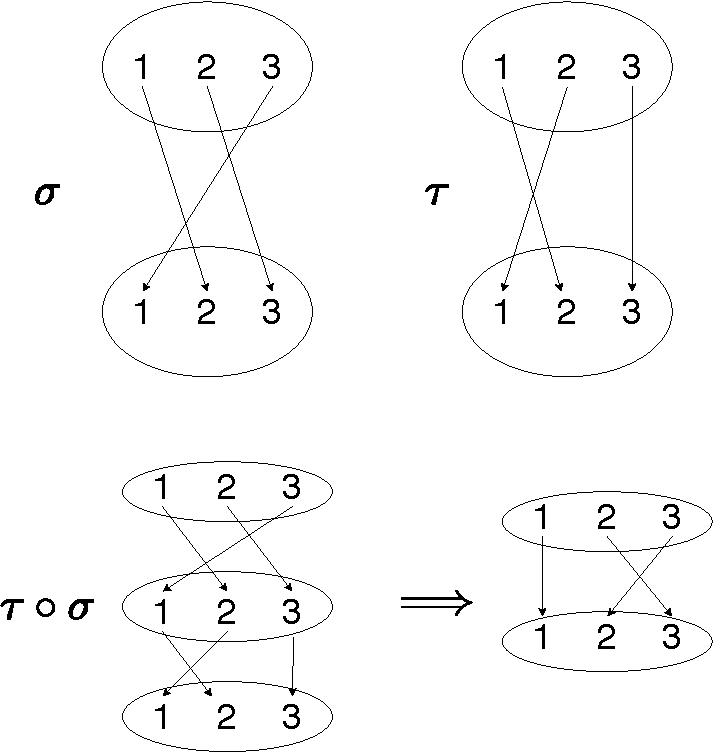
\includegraphics[width=0.75\textwidth]{Figures/composition_diagram-cropped.pdf}
    \caption{Composition Example (Ex 2) where $S=T=U=\{1,2,3\}$}
    \label{fig:composition_example}
\end{figure}
\end{example}
\noindent For example 3, we need one more definition.
\begin{definition}[Power set]
The \textit{power set} $S^{*}$ of a set $S$ is the collection of all subsets of $S$.
\end{definition}
%\noindent\textbf{Defn:} The power set $S^{*}$ of a set $S$ is the collection of all subsets of $S$.\steezybreak\\
\textbf{Example of a power set:} $S=\{1,2,3\}$ has power set $S^*=\{\{1\},\{2\},\{3\},\{2,3\},\{1,3\},\{1,2\},\emptyset,S\}$. If $S$ has $n$ elements, then $S^*$ has $2^n$ elements. \\
\noindent \textbf{\textit{Note(!):}} $S^{*}$'s elements are \textit{subsets} of $S$, not elements of $S$, e.g. $\{\{1\},\{2\}\}\neq \{1,2\}$ and $1\not \in \{\{1\},\{2\}\}$ but $1\in \{1,2\}$, the first set has elements that are \textit{subsets} (of numbers/integers) but the second set has elements that are \textit{numbers/integers}.
\begin{example}
The standard map from a set to its equivalence classes $\tilde{S}^*\subset S^*$.\\ 
Suppose $\sim$ is an equivalence relation on $S$, each equivalence class is a member of $S^*$. Define $\tau:S\rightarrow \tilde{S}^*$ by $\tau(s)=cl(s)$ (i.e. $\tau$ takes $s$ to the class in which it sits/belongs). This map is surjective but not injective.
\end{example}
% \noindent\textbf{Example 3:} The standard map from a set to its equivalence classes.\steezybreak\\
% Suppose $\sim$ is an equivalence relation on $S$, each equivalence class is a member of $S^*$. Define $\tau:S\rightarrow S^*$ by $\tau(s)=cl(s)$ (i.e. $\tau$ takes $s$ to the class in which it sits/belongs). This map is surjective but not injective.\steezybreak\\
% \textbf{Associative Law of Composition (Lemma 1.2.1)}\\
% If $\sigma:S\rightarrow T$ and $\tau: T \rightarrow U$ and $\mu: U \rightarrow V$, then:
% \begin{equation}
%     (\mu\circ\tau)\circ \sigma = \mu \circ (\tau \circ \sigma)\nonumber
% \end{equation}
% \textbf{Proof:} Pick arbitrary $s\in S$\\
% \begin{align}
%     [(\mu\circ \tau)\circ \sigma](s)&= (\mu\circ\tau)(\sigma(s))\nonumber \ \ \ \ \ \ \ (\text{since }(a\circ\sigma) (s) = a(\sigma(s)))\\
%     &= \mu[\tau(\sigma(s))]\nonumber \ \ \ \ \ \ \ \ \ \ (\text{since } \sigma(s)\in T \text{ and } (\mu \circ \tau)(t)= \mu(\tau(t)) \ \forall \ t \in T)\\
%     &= \mu[\tau\circ\sigma(s)]\nonumber \ \ \ \ \ \ \ \ \ \ (\text{since }  (\tau \circ \sigma)(s)= \tau(\sigma(s))  \in U ) \\
%     &= \mu\circ[\tau\circ\sigma(s)].\nonumber \  \ \ \ \ \ (\text{since }  (\mu\circ a)(u)= \mu(a(u))  )\ \ \ \ \ \ \ \blacksquare
% \end{align}
%\newpage
\begin{lemma}[Associative Law of Composition]
%\textbf{ (Lemma 1.2.1)}\\
If $\sigma:S\rightarrow T$ and $\tau: T \rightarrow U$ and $\mu: U \rightarrow V$, then:
\begin{equation}
    (\mu\circ\tau)\circ \sigma = \mu \circ (\tau \circ \sigma)\nonumber
\end{equation}
\textbf{Proof:} Pick arbitrary $s\in S$\\
\begin{align}
    [(\mu\circ \tau)\circ \sigma](s)&= (\mu\circ\tau)(\sigma(s))\nonumber \ \ \ \ \ \ \ (\text{since }(a\circ\sigma) (s) = a(\sigma(s)))\\
    &= \mu[\tau(\sigma(s))]\nonumber \ \ \ \ \ \ \ \ \ \ (\text{since } \sigma(s)\in T \text{ and } (\mu \circ \tau)(t)= \mu(\tau(t)) \ \forall \ t \in T)\\
    &= \mu[\tau\circ\sigma(s)]\nonumber \ \ \ \ \ \ \ \ \ \ (\text{since }  (\tau \circ \sigma)(s)= \tau(\sigma(s))  \in U ) \\
    &= \mu\circ[\tau\circ\sigma(s)].\nonumber \  \ \ \ \ \ (\text{since }  (\mu\circ a)(u)= \mu(a(u))  )\ \ \ \ \ \ \ \blacksquare
\end{align}
\end{lemma}
\begin{lemma}
If $\sigma: S\rightarrow T$, $\tau: T\rightarrow V$
\begin{enumerate}
    \item if both $\sigma$ and $\tau$ are surjective, then $\tau \circ \sigma$ is surjective.
    \item if both $\sigma$ and $\tau$ are injective, then $\tau \circ \sigma$ is injective.
\end{enumerate}
\textbf{Proof:} 1) We will begin by assuming $\sigma$ and $\tau$ are surjective and show this implies $\tau \circ \sigma$ is surjective. Assume $\sigma$ and $\tau$ surjective. Let $v\in V$, $\tau$ surjective means $\exists \ t\in T \ni \tau(t)=v $, similarly, $\sigma$ surjective $\implies$ $\exists \ s\in S \ni \sigma(s)=t$. Then
\begin{equation}
    (\tau \circ \sigma)(s)=\tau[\sigma(s)]=\tau[t]=v\nonumber
\end{equation}
so $s$ is a pre-image of $v$ meaning $\tau\circ \sigma$ is also surjective.

2) Take $s_1,s_2\in S \ni s_1\neq s_2$, then $\sigma$ injective $\implies$ $\sigma(s_1)\neq\sigma(s_2)$. $\tau$ injective $\implies \tau[\sigma(s_1)]\neq \tau[\sigma(s_2)] \implies (\tau \circ \sigma)$ keeps distinct elements distinct (so $\tau \circ \sigma$ is injective). $\blacksquare$
\end{lemma}
% \textbf{Lemma 1.2.2}\\
% If $\sigma: S\rightarrow T$, $\tau: T\rightarrow V$
% \begin{enumerate}
%     \item if both $\sigma$ and $\tau$ are surjective, then $\tau \circ \sigma$ is surjective.
%     \item if both $\sigma$ and $\tau$ are injective, then $\tau \circ \sigma$ is injective.
% \end{enumerate}
% \textbf{Proof:} 1) We will begin by assuming $\sigma$ and $\tau$ are surjective and show this implies $\tau \circ \sigma$ is surjective. Assume $\sigma$ and $\tau$ surjective. Let $v\in V$, $\tau$ surjective means $\exists \ t\in T \ni \tau(t)=v $, similarly, $\sigma$ surjective $\implies$ $\exists \ s\in S \ni \sigma(s)=t$. Then
% \begin{equation}
%     (\tau \circ \sigma)(s)=\tau[\sigma(s)]=\tau[t]=v\nonumber
% \end{equation}
% so $s$ is a pre-image of $v$ meaning $\tau\circ \sigma$ is also surjective.

% 2) Take $s_1,s_2\in S \ni s_1\neq s_2$, then $\sigma$ injective $\implies$ $\sigma(s_1)\neq\sigma(s_2)$. $\tau$ injective $\implies \tau[\sigma(s_1)]\neq \tau[\sigma(s_2)] \implies (\tau \circ \sigma)$ keeps distinct elements distinct (so $\tau \circ \sigma$ is injective). $\blacksquare$ \steezybreak\\
\begin{lemma}
$\sigma :S \rightarrow T$.
\begin{equation}
    \sigma \text{ is a bijection} \iff \exists \ \mu: T\rightarrow S \ni \mu\circ \sigma = I_S \text{ and } \sigma\circ \mu = I_T\nonumber
\end{equation}
(The method of proof for an equivalence $\Leftrightarrow$ is to show each side implies the other)\steezybreak\\
\textbf{Proof:} we will begin with showing the $\Leftarrow$ direction.\\
\textbf{$\Leftarrow$:} \\Assume that $\mu$ exists with the stated properties; show that this forces $\sigma$ to be a bijection. We will begin by showing $\sigma$ is injective through a contradiction \steezybreak\\
\textit{$\sigma$ Inj:} Suppose $\sigma$ is not injective $\implies \exists \ s_1,s_2\in S \ni s_1\neq s_2$ and $\sigma(s_1)=\sigma(s_2)$. But we know $\mu \circ \sigma = I_s$ which means $\mu\circ \sigma (s_1) = \mu\circ \sigma(s_2) = s_1=s_2$ $\Rightarrow\Leftarrow$ $s_1$ and $s_2$ were assumed non-equal!! So $\sigma$ must be injective.\steezybreak\\
Now, we will show that $\sigma$ is also surjective if such a $\mu$ exists.\steezybreak\\
\textit{$\sigma$ Surj:} Take arbitrary $t\in T$. $t= I_t(t)= (\sigma\circ\mu)(t)=\sigma(\mu(t))$ and $\mu(t)\in S$ so $\mu(t)$ serves as a preimage for $t$ under $\sigma$. Therfore $\sigma$ is surjective. \\ 

\noindent Now to show the other implication (i.e. show LHS of Lemma 1.2.3 $\implies$ RHS) \\
\textbf{$\Rightarrow$:} \\ We assume $\sigma$ is a bijection, now we have to:
\begin{enumerate}
    \item Define a rule called $\mu:T\rightarrow S$
    \item Show $\mu$ is a mapping (each element in $T$ should go to exactly one element in $S$)
    \item Verify the defined $\mu$ satisfies the stated composition properties
\end{enumerate}
\textbf{1)} Which element of $S$ should be $\mu(t)$? Well, $\sigma$ surjective $\implies t$ has a pre-image in $S$ or $\exists s\in S \ni \sigma(s)=t$. So let's define $ \mu: T\rightarrow S$ by $\mu(t)=s$ for which $\sigma(s)=t$ (i.e. $\mu(t)$ will always just take $t$ to its pre-image under $\sigma$)\steezybreak\\

\noindent\textbf{2)} Is $\mu$ well-defined (is $\mu$ actually a mapping/function)? Can $t$ have more than one pre-image (this would result in more than one value for $\mu(t)$ making $\mu$ not a function)?\steezybreak\\
NO! $t$ cannot have more than one pre-image because having $s_1\neq s_2$ and $\sigma(s_1)=\sigma(s_2)=t$ would violate injectivity of $\sigma$. So $\mu$ is well-defined.\steezybreak\\

\noindent\textbf{3)} Take $s\in S$, $(\mu\circ \sigma)(s)=\mu(\sigma(s))=\mu(t)=s=I_s(s)$. $\therefore (\mu\circ \sigma)= I_S$\steezybreak\\

Take $t\in T$, $(\sigma\circ \mu)(t)= \sigma(\mu(t))=\sigma(s)=t=I_T(t)$. $\therefore (\sigma\circ \mu) = I_T$. $\blacksquare$ \steezybreak\\

\noindent Notation: In light of its role, $\mu$ is renamed $\sigma^{-1}$ (``$\sigma$ inverse") and we can rewrite the lemma like this:

\begin{equation}
    \sigma:S\rightarrow T \text{ is a bijection } \iff \sigma \text{ has an inverse } \sigma^{-1}: T\rightarrow S \text{ with } (\sigma^{-1}\circ \sigma)= I_S \text{ and } (\sigma \circ \sigma^{-1})=I_T\nonumber
\end{equation}
\end{lemma}\steezybreak
\begin{tcolorbox}
\begin{center}
    $\star\star\star$ \textbf{Read up to this point to Complete Homework 1} $\star\star\star$
\end{center}
\end{tcolorbox}
\steezybreak
% \noindent\textbf{Lemma 1.2.3} $\sigma :S \rightarrow T$.
% \begin{equation}
%     \sigma \text{ is a bijection} \iff \exists \ \mu: T\rightarrow S \ni \mu\circ \sigma = I_S \text{ and } \sigma\circ \mu = I_T\nonumber
% \end{equation}
% (The method of proof for an equivalence $\Leftrightarrow$ is to show each side implies the other)\steezybreak\\
% \textbf{Proof:} we will begin with showing the $\Leftarrow$ direction.\\
% \textbf{$\Leftarrow$:} Assume that $\mu$ exists with the stated properties; show that this forces $\sigma$ to be a bijection. We will begin by showing $\sigma$ is injective through a contradiction \steezybreak\\
% \textit{$\sigma$ Inj:} Suppose $\sigma$ is not injective $\implies \exists s_1,s_2\in S \ni s_1\neq s_2$ and $\sigma(s_1)=\sigma(s_2)$. But we know $\mu \circ \sigma = I_s$ which means $\mu\circ \sigma (s_1) = \mu\circ \sigma(s_2) = s_1=s_2$ $\Rightarrow\Leftarrow$ $s_1$ and $s_2$ were assumed non-equal!! So $\sigma$ must be injective. Now we will show that $\sigma$ is also surjective if such a $\mu$ exists.\steezybreak\\
% \textit{$\sigma$ Surj:} Take arbitrary $t\in T$. $t= I_t(t)= (\sigma\circ\mu)(t)=\sigma(\mu(t))$ and $\mu(t)\in S$ so $\mu(t)$ serves as a preimage for $t$ under $\sigma$. Therfore $\sigma$ is surjective. \steezybreak\\

% \noindent Now to show the other implication (LHS of Lemma 1.2.3 $\implies$ RHS) \steezybreak\\
% \textbf{$\Rightarrow$:}Now we assume $\sigma$ is a bijection, now we have to:
% \begin{enumerate}
%     \item Define a rule called $\mu:T\rightarrow S$
%     \item Show $\mu$ is a mapping (each element in $T$ should go to exactly one element in $S$)
%     \item Verify the defined $\mu$ satisfies the stated composition properties
% \end{enumerate}
% \textbf{1)} Which element of $S$ should be $\mu(t)$? Well, $\sigma$ surjective $\implies t$ has a preimage in $S$ or $\exists s\in S \ni \sigma(s)=t$. So let's define $ \mu: T\rightarrow S$ by $\mu(t)=s$ for which $\sigma(s)=t$ (i.e. $\mu(t)$ will always just take $t$ to its preimage under $\sigma$)\steezybreak\\

% \noindent\textbf{2)} Is $\mu$ well defined? (Is it actually a mapping/function?). Can $t$ have more than one pre-image (this would result in more than one value for $\mu(t)$ making $\mu$ not a function)?\steezybreak\\
% NO! Because having $s_1\neq s_2$ and $\sigma(s_1)=\sigma(s_2)$ would violate injectivity of $\sigma$. So $\mu$ is well-defined.\steezybreak\\

% \noindent\textbf{3)} Take $s\in S$, $(\mu\circ \sigma)(s)=\mu(\sigma(s))=\mu(t)=s=I_s(s)$. $\therefore (\mu\circ \sigma)= I_S$\steezybreak\\

% Take $t\in T$, $(\sigma\circ \mu)(t)= \sigma(\mu(t))=\sigma(s)=t=I_T(t)$. $\therefore (\sigma\circ \mu) = I_T$. $\blacksquare$ \steezybreak\\

% \noindent Notation: In light of its role, $\mu$ is renamed $\sigma^{-1}$ (``$\sigma$ inverse") and we can rewrite the lemma like this:

% \begin{equation}
%     \sigma:S\rightarrow T \text{ is a bijection } \iff \sigma \text{ has an inverse } \sigma^{-1}: T\rightarrow S \text{ with } (\sigma^{-1}\circ \sigma)= I_S \text{ and } (\sigma \circ \sigma^{-1})=I_T\nonumber
% \end{equation}

\section{\texorpdfstring{The Integers (in examples, $a,b,c...\in \mathbb{Z}$)}{The Integers (in examples, a,b,c... elements of Z (the integers)}}
\textbf{Euclidean Algorithm (Axiom):} Given $a$ and $b\neq 0$, $\exists \ q,r \in \mathbb{Z}\ni a= bq+r$ where $0\leq r<|b|$  \\  
We call $b$ the divisor, $q$ the quotient, and $r$ the remainder.\steezybreak\\
\textbf{Examples:}
\begin{example}
\setstackgap{S}{1.5pt}
\stackMath\def\stackalignment{r}
Let $a=143$ and $b=20$\steezybreak\\
\(
\stackunder{%
  20 \stackon[1pt]{\showdiv{143}}{7}%
}{%
  \Shortstack[l]{{\ph{3}\underline{140}} \ph{300}3}%
}
\) $\implies \ \ a=bq+r=143=(20)(7) + 3$ \\
\end{example}

\begin{example}
How about $a=-143$ and $b=20$?

\(
\stackunder{%
  20 \stackon[1pt]{\showdiv{-143}}{-7}%
}{%
  \Shortstack[l]{{\ph{300}\underline{-140}} \ph{3000}-3}%
}
\)   \ \ \ \     !!! not a valid division since $-3$ doesn't fall between 0 and 19... let's try again \smiley \\

\(
\stackunder{%
  20 \stackon[1pt]{\showdiv{-143}}{-8}%
}{%
  \Shortstack[l]{{\ph{000}\underline{-160}} \ph{50000}17}%
}
\)$\implies \ \ a=bq+r=-143=(20)(-8) + 17$ \\
\end{example}

\begin{example}

\noindent How about $a=143$ and $b=-20$?\steezybreak\\
\(
\stackunder{%
  -20 \stackon[1pt]{\showdiv{143}}{-7}%
}{%
  \Shortstack[l]{{\ph{3000}\underline{140}} \ph{300000}3}%
}
\) $\implies \ \ a=bq+r=143=(-20)(-7) + 3$
\steezybreak\\ \\
\begin{definition}[Divides (relation)]
$b\in \Z \ni b\neq 0$. $b$ \textit{divides} $a$ (denoted $b|a$) if $\exists \ m\in \mathbb{Z}\ni a=mb$
\steezybreak\\
\noindent (Note, under Eucl., if $a=b\cdot q + r, \ \ 0\leq r<|b|, \ b\neq 0$, then $b|a \iff r=0$)
\end{definition}
\end{example}

%\noindent\textbf{Defn:} $b\in \Z \ni b\neq 0$. $b$ divides $a$ (denoted $b|a$) if $\exists \ m\in \mathbb{Z}\ni a=mb$ \steezybreak\\
\noindent Here are some useful observations we can make from this new definition.\steezybreak\\
\noindent\textbf{Observation 1:} $b|1\implies b=\pm 1$\\
\textit{Proof:} $b|1$ means $\exists m\in \mathbb{Z}\ni 1=mb$. There are only 2 possible combinations of integers that satisfy $mb=1$, either $m=b=1$ (i.e. $(1)(1)=1$) or $m=b=-1$ (i.e. $(-1)(-1)=1$) $\implies b=\pm 1$ \steezybreak\\
\noindent\textbf{Observation 2:} $a|b$ and $b|a$ $\implies$ $b=\pm a$ \steezybreak\\
\textit{Proof:} $a|b \implies \exists m \in \mathbb{Z} \ni b= ma$. $b|a \implies \exists n \in \mathbb{Z} \ni a= nb$. So $b=ma=mnb$. The first and last expressions ($b=mnb$) imply that $mn=1$, using our previous observation, this forces $m=\pm 1$ $\implies$ $b=\pm a$\steezybreak\\
\noindent\textbf{Observation 3:} $b|0$ is true for any non-zero $b\in \mathbb{Z}$ because $0=0\cdot b$ is an integer multiple of $b$ ($0\in \mathbb{Z}$ is the integer multiple)\steezybreak\\
\noindent\textbf{Observation 4:}  $b|a$ and $b|c$ $\implies$ $b|(\text{any linear combination of }a,c)$ \steezybreak\\
\textit{Proof:} 
\begin{align}
    b|a &\implies \ \ \exists \ m \in \Z \ni a=mb \nonumber \\
    b|c &\implies \ \ \exists \ n \in \Z \ni c=nb \nonumber
\end{align}
Take $r,s\in \Z$, then $ra+sc$ is an arbitrary linear combination of $a,c$.
\begin{align}
    ra+sc=r(mb)+s(nb)=(rm+sn)b\nonumber
\end{align}
lastly we note $(rm+sn)\in \Z$, $\therefore b|(ra+sc)$.
\noindent Ver nice. Ok, lets put these observations in one place for quick reference
\begin{proposition}[Four Observations about Integer Division] 
For integers $b\neq 0$
\begin{enumerate}
    \item $b|1\implies b=\pm 1$
    \item $a|b$ and $b|a$ $\implies b=\pm a$
    \item $b|0 \ \forall \ b \in \Z \ni b\neq 0$
    \item $b|a$ and $b|c$ $\implies$ $b|(ra+sc) \ \forall \ r,s \in \Z$
\end{enumerate}
\end{proposition}
% \noindent\textbf{Four Observations about Division}
% \begin{enumerate}
%     \item $b|1\implies b=\pm 1$
%     \item $a|b$ and $b|a$ $\implies b=\pm a$
%     \item $b|0 \ \forall \ b \in \Z \ni b\neq 0$
%     \item $b|a$ and $b|c$ $\implies$ $b|(ra+sc) \ \forall \ r,s \in \Z$
% \end{enumerate}

\subsection{Dividing Integers and Greatest Common Divisors}
What is the greatest common divisor of $24$ and $36$? Let's list the divisors they have in common:
\begin{equation}
    \pm 1, \pm 2, \pm 3, \pm 4, \pm 6, \pm 12 \nonumber
\end{equation}
Well that seems to be all of them, so the greatest common divisor is the biggest: $12$\steezybreak\\
\begin{definition}[Greatest Common Divisor]
The positive integer $c$ is the \textit{greatest common divisor} of $a$ and $b$ denoted $GCD(a,b)$ provided:
\begin{enumerate}[label=\roman*)]
    \item $c|a$ and $c|b$      \ \ \ \ \ \ \ \ \ \ \ \ \ \ \ \ \ \ \ \ \ \ \ (common)
    \item if $d|a$ and $d|b$, then $d|c$ \ \ \ \ \ \  (biggest)
\end{enumerate}
\end{definition}
% \noindent\textbf{Defn:} The positive integer $c$ is the greatest common divisor of $a$ and $b$ denoted $GCD(a,b)$ provided:
% \begin{enumerate}[i)]
%     \item $c|a$ and $c|b$      (common)
%     \item if $d|a$ and $d|b$, then $d|c$  (biggest)
% \end{enumerate}
\textit{Note:} For the readers who are reviewing with this text and already know some category theory, does the definition of GCD look familiar? Can you think of a category $\mathcal{C}$ where GCD is a categorical product? Using similar reasoning, what must the co-product be in this category? Does this category have a terminal or initial object(s)? If so, what? (hint: $\text{obj}(\mathcal{C})=\Z^+$)
\begin{proposition}[Uniqueness of $GCD(a,b)$]
Suppose $c_1$ and $c_2$ both satisfy the definition of $GCD(a,b) \implies c_1|c_2$ and $c_2|c_1$, so by observation \#2, $c_1=\pm c_2 \implies c_1=c_2$ (because, $c_1,c_2$ assumed positive). So the $GCD(a,b)$ is unique.
\end{proposition}
\begin{example}
$GCD(0,0)$ Does not exist (DNE)
\end{example}
\begin{example}
$GCD(0,7)=7$ because $0$ and $7$ have common factors $\pm 1,\pm 7$; \\
In fact: $GCD(0, b)=|b| \ \ \forall \ b\in \Z\ni b\neq 0$.
\end{example}


\begin{lemma}[Existence of $GCD(a,b)$] 
if $a,b\in \Z$ are not both $0$, then $GCD(a,b)$ exists; in fact, $\exists \ m_0,n_0\in \Z \ni $
\begin{equation}
    GCD(a,b)=m_0 a+n_0 b\nonumber
\end{equation}

\noindent\textbf{Proof:} Let $M= \{ma+nb \ | \ \forall \ m,n,\in \Z \}$
\begin{align}
a&=(1)\cdot a + (0)\cdot b \in M \nonumber \\
b&=(0)\cdot a + (1)\cdot b \in M\nonumber \\
-a&=(-1)\cdot a + (0)\cdot b \in M\nonumber \\
-b&=(0)\cdot a + (-1)\cdot b \in M\nonumber 
\end{align}
At least one of $a,-a,b,-b$ is positive so we may say that $M$ contains positive integers. Let $c$ denote the smallest positive integer in $M$. Then:\\
\begin{equation}
    c=m_0 a +n_0 b \ \ \text{ for some } m_0,n_0\in \Z \nonumber
\end{equation}
\textit{Claim:} $c=GCD(a,b)$. ( to prove this claim we must show $c|a$, $c|b$, and if $d|a$ and $d|b$ then $d|c$.)\\
\textit{Proof:} To begin we note that the Euclidean algorithm can be used to divide any element $\in M$ by $c$. Take arbitrary $m,n \in \Z$, then $ma+nb$ is an arbitrary element of $M$. Eucl. Algorithm $\implies$ $\exists q,r \in \Z\ni (ma+nb)=q\cdot c + r$ where $0\leq r < c$. Now we solve for $r$:
\begin{align}
    r&= (ma+nb)-q\cdot c \nonumber\\
    &= (ma+nb)-q(m_0a +n_0 b) \nonumber\\
    &= (m-qm_0)a+(n- q n_0)b \nonumber\\
    &\therefore r\in M \nonumber
\end{align}
Since $c$ is the \textit{smallest positive integer} in $M$, and $0\leq r < c$ and $r\in M$, this implies that $r=0$.\steezybreak\\
So $c|(ma+nb)$. If $c$ divides everything in $M$, then $c|a$ and $c|b$. Also if $d|a$ and $d|b$ then observation \#4 $\implies$ $d|(\text{the linear combination } m_0a+n_0b)$\steezybreak\\
$\therefore GCD(a,b)=c=m_0a+n_0b \ \ \ \ \blacksquare$\steezybreak\\
\end{lemma}
% \textbf{Lemma 1.3.1 (Existence of $GCD(a.b)$):} if $a,b\in \Z$ are not both $0$, then $GCD(a,b)$ exists; in fact, $\exists \ m_0,n_0\in \Z \ni $\\
% \begin{equation}
%     GCD(a,b)=m_0 a+n_0 b\nonumber
% \end{equation}

% \noindent\textbf{Proof:} Let $M= \{ma+nb|\forall m,n,\in \Z \}$\steezybreak\\
% $a=(1)\cdot a + (0)\cdot b \in M$\\
% $b=(0)\cdot a + (1)\cdot b \in M$\\
% $-a=(-1)\cdot a + (0)\cdot b \in M$\\
% $-b=(0)\cdot a + (-1)\cdot b \in M$\\

% At least one of $a,-a,b,-b$ is positive so we may say that $M$ contains positive integers. Let $c$ denote the smallest positive integer in $M$. Then:\\
% \begin{equation}
%     c=m_0 a +n_0 b \ \ \text{ for some } m_0,n_0\in \Z \nonumber
% \end{equation}
% \textit{Claim:} $c=GCD(a,b)$. ( to prove this claim we must show $c|a$, $c|b$, and if $d|a$ and $d|b$ then $d|c$.)\\
% \textit{Proof:} To begin we note that the Euclidean algorithm can be used to divide any element $\in M$ by $c$. Take arbitrary $m,n \in \Z$, then $ma+nb$ is an arbitrary element of $M$. Eucl. Algorithm $\implies$ $\exists q,r \in \Z\ni (ma+nb)=q\cdot c + r$ where $0\leq r < c$. Now we solve for $r$:
% \begin{align}
%     r&= (ma+nb)-q\cdot c \nonumber\\
%     &= (ma+nb)-q(m_0a +n_0 b) \nonumber\\
%     &= (m-qm_0)a+(n- +q n_0)b \nonumber\\
%     &\therefore r\in M
% \end{align}
% Since $c$ is the \textit{smallest positive integer} in $M$, and $0\leq r < c$ and $r\in M$, this implies that $r=0$.\steezybreak\\
% So $c|(ma+nb)$. If $c$ divides everything in $M$, then $c|a$ and $c|b$. Also if $d|a$ and $d|b$ then observation \#4 $\implies$ $d|(\text{the linear combination } m_0a+n_0b)$\steezybreak\\
% $\therefore GCD(a,b)=c=m_0a+n_0b \ \ \ \ \blacksquare$\steezybreak\\
\begin{example}
Find $GCD(1812,1200)$, to do this, we can use the euclidean algorithm to find GCD by first dividing $a$ by $b$ and then continually dividing the divisor by the remainder (Note: here we will represent $a$ as $a=qb+r$, i.e. writing the quotient first, this is allowed because integers are commutative under multiplication, this view is convenient for the next few examples):
\begin{align}
    1812 &=1\cdot1200+612\nonumber\\
    1200 &=1\cdot612+588 \nonumber\\
    612 &=1\cdot588+24 \nonumber\\
    588 &=24\cdot24+12 \nonumber\\
    24 &=2\cdot12+0 \nonumber
\end{align}
The GCD will be the second to last remainder (last remainder is always 0, i.e. you are done when the remainder =0) so in this case the GCD is $12$. This method is nice because reading these divisions from bottom to top ($\big\uparrow$) shows $12$ is a common divisor of $a$ and $b$ and reading from top to bottom ($\big\downarrow$) shows it is the greatest (since we stop the first time a zero remainder [i.e. a common divisor] appears).
\end{example}
% \textbf{Example 1} Find $GCD(1812,1200)$, to do this, we can use the euclidean algorithm to find GCD by first dividing $a$ by $b$ and then continually dividing the divisor by the remainder:
% \begin{align}
%     1812 &=1\cdot1200+612\nonumber\\
%     1200 &=1\cdot612+588 \nonumber\\
%     612 &=1\cdot588+24 \nonumber\\
%     588 &=24\cdot24+12 \nonumber\\
%     24 &=2\cdot12+0 \nonumber\\
% \end{align}
% The GCD will be the second to last remainder (last remainder is always 0, i.e. you are done when the remainder =0) so in this case the GCD is $12$. This method is nice because reading these divisions from bottom to top ($\big\uparrow$) shows $12$ is a common divisor of $a$ and $b$ and reading from top to bottom ($\big\downarrow$) shows it is the greatest (since we stop the first time a zero remainder [i.e. a common divisor] appears).\steezybreak\\
\begin{example}
Find $m,n\in \Z \ni GCD(71,31)=m\cdot 71+n\cdot 31$.\steezybreak\\
\begin{align}
    71&= 2\cdot 31+9 \ \implies 9=71-2\cdot 31 \nonumber\\
    31&= 3\cdot 9+4 \ \implies 4=31-3\cdot 9\nonumber\\
    9&= 2\cdot 4+1 \ \implies 1=9-2\cdot 4\nonumber\\
    4&= 4\cdot 1+0 \nonumber
\end{align}
So the $GCD(71,31)=1$ and using the implications we gathered along the way we can back-substitute for an expression in terms of $71$ and $31$
\begin{align}
    1&=9-2[31-3\cdot 9]\nonumber \\
    &=7\cdot 9- 2\cdot 31\nonumber \\
    &=7\cdot [71-2\cdot 31]- 2\cdot 31\nonumber \\
    &=7\cdot 71+ (-16)\cdot 31\nonumber 
\end{align}
\end{example}
% \noindent \textbf{Example 2} Find $m,n\in \Z \ni GCD(71,31)=m\cdot 71+n\cdot 31$.\steezybreak\\
% \begin{align}
%     71&= 2\cdot 31+9 \ \implies 9=71-2\cdot 31 \nonumber\\
%     31&= 3\cdot 9+4 \ \implies 4=31-3\cdot 9\nonumber\\
%     9&= 2\cdot 4+1 \ \implies 1=9-2\cdot 4\nonumber\\
%     4&= 4\cdot 1+0 \nonumber\\
% \end{align}
% So the $GCD(71,31)=1$ and using the implications we gathered along the way we can back-substitute for an expression in terms of $71$ and $31$
% \begin{align}
%     1&=9-2[31-3\cdot 9]\nonumber \\
%     &=7\cdot 9- 2\cdot 31\nonumber \\
%     &=7\cdot [71-2\cdot 31]- 2\cdot 31\nonumber \\
%     &=7\cdot 71+ (-16)\cdot 31\nonumber \\
% \end{align}
\newpage
\subsection{Alternate Method with $2\times 2$ Matrices}
Rather than performing repeated back-substitutions, there is a clean way we can implement this same procedure using $2\times 2$ matrices. Using our example from before,\\
\begin{align}
    71&= 2\cdot 31+9 \ \ \ \ \text{Let's denote }2=q_1\nonumber\\
    31&= 3\cdot 9+4 \ \ \ \ \ \ \text{Let's denote }3=q_2\nonumber\\
    9&= 2\cdot 4+1 \ \ \ \ \ \ \text{Let's denote }2=q_3 \ \text{ (don't use 0 remainder quotient)}\nonumber\\ \hline
    4&= 4\cdot 1+0 \nonumber
\end{align}
In this approach, instead of repeatedly back-substituting ourselves, we take a consecutive product of matrices whose values are determined by the quotients we discover by running the eucl. alg. The matrices will have the form:
\begin{equation}
   M=
  \left( {\begin{array}{cc}
   0 & 1 \\
   1 & -q \\
  \end{array} } \right)
\nonumber
\end{equation}
\textbf{Ex:}
\begin{align}
  \left( {\begin{array}{cc}
   0 & 1 \\
   1 & -q_3 \\
  \end{array} } \right)\left( {\begin{array}{cc}
   0 & 1 \\
   1 & -q_2 \\
  \end{array} } \right)\left( {\begin{array}{cc}
   0 & 1 \\
   1 & -q_1 \\
  \end{array} } \right) 
  =\left( {\begin{array}{cc}
   0 & 1 \\
   1 & -2 \\
  \end{array} } \right)\left( {\begin{array}{cc}
   0 & 1 \\
   1 & -3 \\
  \end{array} } \right)\left( {\begin{array}{cc}
   0 & 1 \\
   1 & -2 \\
  \end{array} } \right)=\left( {\begin{array}{cc}
   -3 & 7 \\
   7 & -16 \\
  \end{array} } \right) \nonumber\\
  \therefore 1= (7)*71+(-16)*31
\nonumber
\end{align}
Why does this work? Consider again the equation:
\begin{align}
    a=qb+r \nonumber
\end{align}

when finding the GCD, we begin by dividing $a$ by $b$ and recording the quotient and remainder that solved the above equation, we then replace our divisor with the last remainder and $a$ with the last divisor and continue in this way until we find a remainder that is equal to $0$., i.e. we enforce:
\begin{align}
    a_0=a, d_0=b \ \ \ (a\text{ and divisor }b)\nonumber\\
    d_{n+1}= r_n  \ \ \ (\text{ next divisor last remainder })\nonumber \\
    a_{n+1}= d_n \ \ \ (\text{ next dividend is last divisor })\nonumber 
\end{align}
One step of these divisions could be represented in matrix notation by using the following,
\begin{equation}
  \left( {\begin{array}{cc}
   0 & 1 \\
   1 & -q \\
  \end{array} } \right)\left( {\begin{array}{c}
   a\\
   b
  \end{array} } \right)=\left( {\begin{array}{c}
   b\\
   r
  \end{array} } \right)
\nonumber
\end{equation}
We can see that if we record the quotients as we go through the process, we can immediately find the linear combination that gives us the $GCD(a,b)$ in terms of $a$ and $b$ because it will simply be the coefficients in the last row of the product of these quotient matrices (i.e. $M$-like matrices).

\subsection{Primes and Prime Factorization of Integers}
\begin{definition}[Prime Numbers and Co-prime (Relatively prime) Pairs of Numbers]
\begin{enumerate}
    \item $a$ and $b$ are \textit{relatively prime} if $GCD(a,b)=1$.
    \item $p>1$ is \textit{prime} if its \textit{only} divisors are $\pm 1$ and $\pm p$.
\end{enumerate}
\end{definition}
% \textbf{Defn (s):}
% \begin{enumerate}
%     \item $a$ and $b$ are relatively prime if $GCD(a,b)=1$.
%     \item $p>1$ is prime if its \textit{only} divisors are $\pm 1$ and $\pm p$.
% \end{enumerate}
\begin{proposition}[a.k.a. Proposition $\star$] 
$p$ is prime $\iff$ $\forall \ n \in \Z $, either $p|n$ or $p$ and $n$ are relatively prime.\\
\textit{Proof:} \\
\textbf{$\Rightarrow :$}\\
Assume $p$ is prime; take arbitrary $n\in\Z$, $GCD(p,n)|p\ \ \implies \ GCD(p,n)$ is $1$ or $p$. If $GCD(p,n)=1$ then we are done since $p,n$ are relatively prime, if $GCD(p,n)=p$ then because $GCD(p,n)|n$ we have $p|n$.\steezybreak\\
\textbf{$\Leftarrow :$}\\
Assume $\forall n \in \Z$, either $p|n$ or $GCD(p,n)=1$. We must show that the only divisors of $p$ are $\pm 1, \pm p$. Let $d$ be a divisor of $p$ (so $d|p$). If we consider our hypothesis again, now thinking of $d$ as one of the $n\in\Z$ we have that either $p|d$ or $GCD(p,d)=1$. If $p|d$ then observation \#2 $\implies$ $d=\pm p$. If $GCD(p,d)=1$ then since $d$ is a common divisor of both $p$ (by assumption on $d$) and $d$ (obvious) and because the $GCD(p,d)$ is the greatest such divisor we have that $d|GCD(p,d)=d|1$ so by observation \# 1 we can conclude $d=\pm 1$. $\therefore \ p$ is prime. $\blacksquare$
\end{proposition}
% \textbf{Proposition $\star$:} $p$ is prime $\iff$ $\forall \ n \in \Z $, either $p|n$ or $p$ and $n$ are relatively prime.\\
% \textit{Proof:} \\
% \textbf{$\Rightarrow :$}\\
% Assume $p$ is prime; take arbitrary $n\in\Z$, $GCD(p,n)|p\ \ \implies \ GCD(p,n)$ is $1$ or $p$. If $GCD(p,n)=1$ then we are done since $p,n$ are relatively prime, if $GCD(p,n)=p$ then because $GCD(p,n)|n$ we have $p|n$.\steezybreak\\
% \textbf{$\Leftarrow :$}\\
% Assume $\forall n \in \Z$, either $p|n$ or $GCD(p,n)=1$. We must show that the only divisors of $p$ are $\pm 1, \pm p$. Let $d$ be a divisor of $p$ (so $d|p$). If we consider our hypothesis again, now thinking of $d$ as one of the $n\in\Z$ we have that either $p|d$ or $GCD(p,d)=1$. If $p|d$ then observation \#2 $\implies$ $d=\pm p$. If $GCD(p,d)=1$ then since $d$ is a common divisor of both $p$ (by assumption on $d$) and $d$ (obvious) and because the $GCD(p,d)$ is the greatest such divisor we have that $d|GCD(p,d)=d|1$ so by observation \# 1 we can conclude $d=\pm 1$. $\therefore \ p$ is prime. $\blacksquare$\steezybreak\\
\begin{lemma}
If $a$ is relatively prime to $b$ and $a|(b\cdot c)$, then $a|c$. \\
\textit{Proof:} $a,b$ rel. prime $\implies$ $GCD(a,b)=1$, by Lemma 1.3.1 $\exists m,n \in \Z \ni 1= GCD(a,b)=ma+nb$. Now if we multiply both sides of this expression by $c$ we have:
\begin{align}
    c=mac+nbc\nonumber
\end{align}
Now, certainly $a|a$, and from our hypothesis we have that $a|(bc)$ so by observation \# 4 about divisions, $a|(m\underline{a}c+ n\underline{bc})$, i.e. $a|c \ \ \blacksquare$ \steezybreak\\
\end{lemma}
% \noindent \textbf{Lemma 1.3.2:} If $a$ is relatively prime to $b$ and $a|(b\cdot c)$, then $a|c$. \\
% \textit{Proof:} $a,b$ rel. prime $\implies$ $GCD(a,b)=1$, by Lemma 1.3.1 $\exists m,n \in \Z \ni 1= GCD(a,b)=ma+nb$. Now if we multiply both sides of this expression by $c$ we have:
% \begin{align}
%     c=mac+nbc\nonumber
% \end{align}
% Now, certainly $a|a$, and from our hypothesis we have that $a|(bc)$ so by observation \# 4 about divisions, $a|(m\underline{a}c+ n\underline{bc})$, i.e. $a|c \ \ \blacksquare$ \steezybreak\\
\setcounter{dummy_lemma}{1}
\begin{corollary}
If $p$ is prime and $p|n_1n_2...n_K,\ \ n_i\in \Z$, then $p|n_i$ for at least one $i \in \{1,2,3,...,K\}$.\\
\textit{Proof:} By Prop. $\star$, either $p|n_1$ or $GCD(p,n_1)=1$. If $GCD(p,n_1)=1$ then Lemma 1.3.2 $\implies$ $p|n_2n_3...n_K$. Continue applying $\star$, if $GCD(p,n_i)=1$ for all $i$'s up to $K-1$ (i.e. $\forall \ 1\leq i\leq K-1$), then by Lemma 1.3.2 $p|n_K\ \ \ \ \blacksquare$
\end{corollary}
% \noindent\textbf{Corollary:} If $p$ is prime and $p|n_1n_2...n_K,\ \ n_i\in \Z$, then $p|n_i$ for at least one $i \in \{1,2,3,...,K\}$.\\
% \textit{Proof:} By prop $\star$, either $p|n_1$ or $GCD(p,n_1)=1$. If $GCD(p,n_1)=1$ then Lemma 1.3.2 $\implies$ $p|n_2n_3...n_K$. Continue applying $\star$, if $GCD(p,n_i)=1$ for all $i$'s up to $K-1$ (i.e. $\forall \ 1\leq i\leq K-1$), then by Lemma 1.3.2 $p|n_K\ \ \ \ \blacksquare$ \steezybreak\\
\setcounter{dummy}{0}
\begin{theorem}[Unique Factorization] 
Any integer $a>1$ can be factorized uniquely:
\begin{align}
    a=p_1^{\alpha_1}p_2^{\alpha_2}p_3^{\alpha_3}...p_t^{\alpha_t}\nonumber
\end{align}
Where $p_1>p_2>p_3>...>p_t$ are primes for each $\alpha_i>0$.\steezybreak\\
\noindent\textit{Proof:} We will hold off on the proof of this for now and we will prove it later in greater generality.\steezybreak\\
\end{theorem}

\textbf{Example:} $2520=60\cdot 42 = 7^1\cdot 5^1\cdot 3^2 \cdot 2^3$. 
\subsection{Congruence Mod N}
\begin{definition}[Congruence mod N]
$n\in \Z$; $a$ is \textit{congruent} to $b$ modulo $n$ iff $n|a-b$.\\
\textit{Notation:} 
\begin{align}
    a\equiv b \mod n &\iff n|(a-b) \nonumber \\
    &\iff \exists \ m\in \Z \ni a-b=mn \ \ \ (\text{i.e. } a=b+mn) \nonumber \\
    &\iff a \text{ is } b \text{ plus an integer multiple of } n \nonumber
\end{align}
\end{definition}
% \textbf{Defn:} $n\in \Z$; $a$ is congruent to $b$ modulo $n$ iff $n|a-b$.\\
% \textit{Notation:} 
% \begin{align}
%     a\equiv b \mod n &\iff n|(a-b) \nonumber \\
%     &\iff \exists \ m\in \Z \ni a-b=mn \ \ \ (\text{i.e. } a=b+mn) \nonumber \\
%     &\iff a \text{ is } b \text{ plus an integer multiple of } n \nonumber
% \end{align}
\begin{example}
Which integers $a$ are congruent to $26$ mod $12$? Well the last line in the definition above says we just need to take all the integer multiples of 12 (i.e. $12\Z$) and add $26$ to each:
\begin{align}
    12\Z= \{...,-36,-24,-12,0,12,24,36,...\}\nonumber\\
    12\Z+26= \{...,-10,2,14,26,38,50,62,...\}\nonumber
\end{align}
\textit{Notation:} To express that $-10$ is in the list we write:
\begin{equation}
    -10\equiv 26 \mod 12 \nonumber
\end{equation}
\end{example}
% \textbf{Example: } $26 \mod 12$, what integers are congruent to $26$ mod $12$? Take multiples of 12 (i.e. $12\Z$) and add $26$ to each:
% \begin{align}
%     12\Z= \{...,-36,-24,-12,0,12,24,36,...\}\nonumber\\
%     12\Z+26= \{...,-10,2,14,26,38,50,62,...\}\nonumber
% \end{align}
% \textit{Notation:} To express that $-10$ is in the list we write:
% \begin{equation}
%     -10\equiv 26 \mod 12 \nonumber
% \end{equation}
\begin{lemma}[Part 1] 
Congruence mod $n$ is an equivalence relation on the integers.\steezybreak\\
\textit{Proof:} Let $a,b,c\in \Z$
\begin{enumerate}
    \item \textit{Reflexivity:} $a\equiv a\mod n \iff n|(a-a) \iff n|0$. By observation \# 3, $n|0$\\
    $\therefore a\equiv a\mod n$\\
    $\therefore \ \ \ \equiv \mod n$ is reflexive\\
    \item \textit{Symmetry:} \\
    $a\equiv b\mod n \iff n|(a-b) \iff \exists \ k \in \Z \ni a-b=k\cdot n \iff b-a=(-k)\cdot n \ \ \ (\text{note } -k\in \Z) \implies n|(b-a)$\\
    $\therefore \ b\equiv a \mod n$
    \item \textit{Transitivity:} Assume $a\equiv b \mod n$ and $b\equiv c\mod n$. This implies two things:
    \begin{align}
        a\equiv b\mod n \iff n|(a-b) \nonumber\\
        b\equiv c\mod n \iff n|(b-c) \nonumber
    \end{align}
    Using these together with observation \# 4 we see $\implies$ $n|(a-b)+(b-c)=a-c$\\
    $\therefore a\equiv c \mod n.\ \ \ \ \ \ \blacksquare$
\end{enumerate}
\end{lemma}
% \textbf{Lemma 1.3.3 (Pt. 1):} Congruence mod $n$ is an equivalence relation on the integers.\steezybreak\\
% \textit{Proof:} Let $a,b,c\in \Z$
% \begin{enumerate}
%     \item \textit{Reflexivity:} $a\equiv a\mod n \iff n|(a-a) \iff n|0$. By observation \# 3, $n|0$\\
%     $\therefore a\equiv a\mod n$\\
%     $\therefore \ \ \ \equiv \mod n$ is reflexive\\
%     \item \textit{Symmetry:} $a\equiv b\mod n \iff n|(a-b) \iff \ \exists \ k \in \Z \ni a-b=k\cdot n \iff b-a=(-k)\cdot n (\text{note } -k\in \Z) \implies n|(b-a)$\\
%     $\therefore \ b\equiv a \mod n$
%     \item \textit{Transitivity:} Assume $a\equiv b \mod n$ and $b\equiv c\mod n$. This implies two things:
%     \begin{align}
%         a\equiv b\mod n \iff n|(a-b) \nonumber\\
%         b\equiv c\mod n \iff n|(b-c) \nonumber
%     \end{align}
%     Using these togethern with observation \# 4 we see $\implies$ $n|(a-b)+(b-c)=a-c$\\
%     $\therefore a\equiv c \mod n \ \ \blacksquare$
% \end{enumerate}
\begin{example}
Let's take a look at congruence mod $6$ ($\equiv \mod 6$).
\begin{align}
    a\sim b &\iff a\equiv b\mod 6 \nonumber \\
    &\iff 6|(a-b) \nonumber \\
    &\iff \exists \ k \in \Z \ni a-b=6k \ \ (\text{i.e. } a=b+6k) \nonumber 
\end{align}
Let's have a look at the equivalence classes under this equivalence relation:
\begin{align}
    cl(0)&=\{0+6k|k\in \Z \}= 6\Z \nonumber \\
    cl(1)&=\{1+6k|k\in \Z \}= 1+6\Z= \{...,-17,-11,-5,1,7,13,...\} \nonumber \\
    cl(2)&=\{2+6k|k\in \Z \}= 2+6\Z= \{...,-16,-10,-4,2,8,14,...\} \nonumber 
\end{align}
Continuing in this way it is clear that the equivalence relation $\equiv \mod 6$ partitions $\Z$ into 6 equivalence classes. Also note that any member of an equivalence class can be used to name that class, e.g. under this relation $cl(-17)=cl(7)=cl(1)$, another example: 
\begin{align}
    cl(248) \implies
\stackunder{%
  6 \stackon[1pt]{\showdiv{248}}{41}%
}{%
  \Shortstack[l]{{\ph{30}\underline{240}} \ph{300}\underline{08} \text{r=}2}%
}\nonumber
\end{align}
so $cl(248)=cl(2)$ under $\equiv\mod 6$.\steezybreak\\
\textit{Notation:} The equivalence classes under $\equiv \mod n$ are commonly written in terms of the elements belonging to the class using ``square bracket notation" like so: $[a]=cl(a)$ represents the equivalence class of element $a$. In our previous example we would say that $[248]=[2]$ under $\equiv \mod 6$\\
\end{example}
% \textbf{Example} Let's take a look at congruence mod $6$ ($\equiv \mod 6$).
% \begin{align}
%     a\sim b &\iff a\equiv b\mod 6 \nonumber \\
%     &\iff 6|(a-b) \nonumber \\
%     &\iff \exists \ k \in \Z \ni a-b=6k \ \ (\text{i.e. } a=b+6k) \nonumber \\
% \end{align}
% Let's have a look at the equivalence classes under this equivalence relation:
% \begin{align}
%     cl(0)&=\{0+6k|k\in \Z \}= 6\Z \nonumber \\
%     cl(1)&=\{1+6k|k\in \Z \}= 1+6\Z= \{...,-17,-11,-5,1,7,13,...\} \nonumber \\
%     cl(2)&=\{2+6k|k\in \Z \}= 2+6\Z= \{...,-16,-10,-4,2,8,14,...\} \nonumber \\
% \end{align}
% Continuing in this way it is clear that the equivalence realtion $\equiv \mod 6$ partitions $\Z$ into 6 equivalence classes. Also note that any member of an equivalence class can be used to name that class, e.g. under this relation $cl(-17)=cl(7)=cl(1)$, another example: 
% \begin{align}
%     cl(248) \implies
% \stackunder{%
%   6 \stackon[1pt]{\showdiv{248}}{41}%
% }{%
%   \Shortstack[l]{{\ph{30}\underline{240}} \ph{300}\underline{08} \text{r=}2}%
% }\nonumber
% \end{align}
% so $cl(248)=cl(2)$ under $\equiv \mod 6$.\steezybreak\\
% \textit{Notation:} The equivalence classes under $\equiv \mod n$ are commonly written in terms of the elements belonging to the class using ``square bracket notation" like so: $[a]=cl(a)$ represents the equivalence class of element $a$. In our previous example we would say that $[248]=[2]$ under $\equiv \mod 6$\\
\setcounter{dummy_lemma}{2}
\begin{lemma}[Part 2] 
$\equiv \mod n$ partitions $\Z$ into $n$ distinct equivalence classes:
\begin{align}
    [0],[1],[2],...,[n-1]\nonumber
\end{align}
The set of these classes is denoted $\Z_n=\{[0],[1],[2],...,[n-1]\}$.
\begin{align}
    a\equiv b\mod n \iff n|(a-b) \nonumber 
\end{align}
$\equiv \mod n$ is an equivalence relation on $\Z$ with classes:
\begin{align}
    [0]&= n\Z=\{kn|k\in \Z\} \nonumber\\
    [1]&= 1+n\Z=\{kn+1|k\in \Z\} \nonumber\\
    &\vdots \nonumber \\
    [n-1]&= (n-1)+n\Z = \{kn+(n-1)|k\in \Z \} \nonumber
\end{align}

\textit{Proof:} We wish to show that the equivalence relation $\equiv\mod n$ from Part 1, partitions $\Z$ into $n$ distinct equivalence classes. Thm 1.1.1 already guarantees that $\equiv\mod n$ partitions $\Z$ since it is an equivalence relation (Part 1 of L 1.3.3). All that remains to show is that there could be no more than $n$ classes and that those $n$ potential classes are in fact all distinct. The example above (Example 1.3.9) almost serves as proof on its own if you think of general $n$ rather than $n=6$ but we will be a little more clear here. \steezybreak\\
\noindent Let the equivalence class, under this relation, of $a$ be denoted by $[a]$ 
we call it the congruence class $\equiv\mod n$ of $a$. Given any integer $a$, by the
Euclidean algorithm, $a = kn + r$ where $0 \leq r < n$. But then, $a \in [r]$ and
so $[a] = [r]$. Thus there are at most $n$ distinct congruence classes; namely,
$[0], [1], ... , [n- 1]$. Furthermore, these classes are distinct, we will show this through a contradiction: Suppose $[i] = [j]$ with $0 \leq i < j < n$ (i.e. $i$, $j$ distinct and both are members of the set $\{0,1,2,...,n-1\}$, then $n | (j - i)$ where $j - i$ is a positive integer less than $n$, which is obviously impossible! (how could $n$ divide a number that is \textit{strictly} smaller than it but greater than zero?!). $\Rightarrow\Leftarrow$ Consequently, there are exactly the $n$ distinct congruence classes $[0], [1], ... , [n - 1]. \ \ \blacksquare$
\end{lemma}

$\Z_n=\{[0],[1],[2],...,[n-1]\}$.\\
\noindent We will define addition and multiplication on $\Z_n$ as follows; we will show these operations are well defined for our equivalence classes in Part 3 of the Lemma:
\begin{align}
    [a]+[b]&=[a+b] \nonumber \\
    [a]\cdot[b]&=[a\cdot b] \nonumber
\end{align}
% \noindent\textbf{Lemma 1.3.3 (Pt. 2):} $\equiv \mod n$ partitions $\Z$ into $n$ distinct equivalence classes:
% \begin{align}
%     [0],[1],[2],...,[n-1]\nonumber
% \end{align}
% The set of these classes is denoted $\Z_n=\{[0],[1],[2],...,[n-1]\}$.
% \begin{align}
%     a\equiv b\mod n \iff n|(a-b) \nonumber \\
% \end{align}
% $\equiv \mod n$ is an equivalence relation on $\Z$ with classes:
% \begin{align}
%     [0]&= n\Z=\{kn|k\in \Z\} \nonumber\\
%     [1]&= 1+\Z=\{kn+1|k\in \Z\} \nonumber\\
%     &\vdots \nonumber \\
%     [n-1]&= (n-1)+\Z = \{kn+(n-1)|k\in \Z \}
% \end{align}
% $\Z_n=\{[0],[1],[2],...,[n-1]\}$.\\
% \noindent We will define addition and multiplication on $\Z_n$ as follows:
% \begin{align}
%     [a]+[b]=[a+b] \nonumber \\
%     [a]\cdot[b]=[a\cdot b] \nonumber
% \end{align}
\begin{example}
In $\Z_{12}=\{[0],[1],...,[11]\}$.
\begin{align}
    [7]+[4]&=[11]\nonumber \\
    [7]+[8]=[7+8]=[15]&=[3] \ \ \ \ \ \text{throw away multiples of 12 and keep only the remainder.}\nonumber \\
    [7]\cdot[8]=[7\cdot 8]=[56]&=[8] \nonumber
\end{align}
\end{example}
% \textbf{Example:} In $\Z_12=\{[0],[1],...,[11]\}$.
% \begin{align}
%     [7]+[4]&=[11]\nonumber \\
%     [7+8]&=[15]=[3] \ \ \ \ \ \text{throw away multiples of 12 and keep only the remainder.}\nonumber \\
%     [7][8]&=[7\cdot 8]=[56]=[8] \nonumber
% \end{align}
\noindent So we have defined an ``addition" and ``multiplication" for equivalence classes  $[a],[b],[c], ...$ in terms of individual elements $a,b,c$  of classes like so:
\begin{align}
    [a]+[b]&=[a+b] \nonumber \\
    [a]\cdot[b]&=[a\cdot b] \nonumber
\end{align}
%\newpage
Are these operations well-defined?  What could go wrong? Have a look at Figure \ref{fig:Bad_partition}\steezybreak\\
\newpage
\begin{figure}[h!]
    \centering
    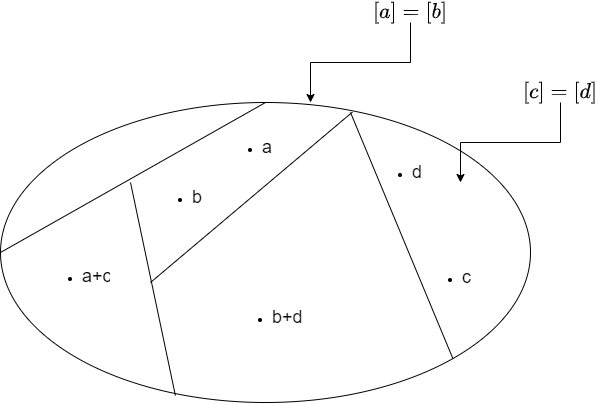
\includegraphics[width=0.6\textwidth]{Figures/partitin_equiv_example.png}
    \caption{Could this happen ($a$ and $b$ are in the same class and $d$ and $c$ are in the same class but $a+c$ and $b+d$ end up in different classes)? We will show this can never happen (i.e. that the operations are well defined).}
    \label{fig:Bad_partition}
\end{figure}

\noindent We must show that if $a$ and $b$ are the same class and $c$ and $d$ are the sample class, then $[a+c]=[b+d]$ \textit{and} $[a\cdot c]=[b\cdot d]$. We show this with the last part of Lemma 1.3.3.
\setcounter{dummy_lemma}{2}
\begin{lemma}[Part 3]
If $a\equiv b\mod n$ and $c\equiv d\mod n$, then $a+c\equiv b+d\mod n$ AND $a\cdot c\equiv b\cdot d \mod n$.\\
\textit{Proof:}
\begin{align}
a\equiv b\mod n \iff n |(a-b)\nonumber\\
c\equiv d\mod n \iff n |(c-d)\nonumber
\end{align}
Then by Observation \#4, $n|a-b+c-d=(a+c)-(b+d)$ (i.e. $n$ divides the linear combination of $a-b$ and $c-d$ so $a+c\equiv b+d\mod n$. Using observation \# 4 again, we can infer the $n|(a-b)c+(c-d)b=ac-bd$ so $ac\equiv bd\mod n \ \ \blacksquare$\\
\end{lemma}

% \textbf{Lemma 1.3.3 (Pt. 3)} If $a\equiv b\mod n$ and $c\equiv d\mod n$, then $a+c\equiv b+d\mod n$ AND $a\cdot c\equiv b\cdot d \mod n$.\\
% \textit{Proof:}
% \begin{align}
% a\equiv b\mod n \iff n |(a-b)\nonumber\\
% c\equiv d\mod n \iff n |(c-d)\nonumber
% \end{align}
% Then by Observation \#4, $n|a-b+c-d=(a+c)-(b+d)$ (i.e. $n$ divides the linear combination of $a-b$ and $c-d$ so $a+c\equiv b+d\mod n$. Using observation \# 4 again, we can infer the $n|(a-b)c+(c-d)b=ac-bd$ so $ac\equiv bd\mod n \ \ \blacksquare$\\
\noindent After having read all three parts of Lemma 1.3.3, one might consider the specific case when $n=2$ again. We see that the "parity", i.e. the odd-ness or even-ness of an integer, exactly corresponds to the two possible equivalence classes for an integer $a\in \Z$ under the relation $\equiv\mod 2$. That is,
\begin{align}
    a\sim0 \iff 2|a-0 \iff 2|a &\iff a \text{ is even} \nonumber \\
    a\sim1 \iff 2|a-1 \iff a-1 \text{ is even} &\iff a \text{ is odd} \nonumber
\end{align}
In this way, we can see that the equivalence relation $\equiv\mod n$ generalizes the notion of "parity" to $n$ remainder classes, rather than just $+1$ or $+0$ remainder classes like congruence $\mod 2$ does. Similarly, Part 3 of this lemma specifically, vastly generalizes the well-established facts that: 
\begin{align}
    \text{even}+\text{even}&=\text{even} &\iff &[0]+[0]=[0] \text{ \ \ and }& \text{even}\cdot \text{even} &=\text{even} &\iff [0]\cdot [0]=[0]\nonumber \\
    \text{even}+\text{odd}&=\text{odd} &\iff &[0]+[1]=[1] \text{ \ \ and }& \text{even}\cdot \text{odd} &=\text{even} &\iff [0]\cdot [1]=[0] \nonumber \\
    \text{odd}+\text{even}&=\text{odd} &\iff &[1]+[0]=[0] \text{ \ \ and }& \text{odd}\cdot \text{even} &=\text{even} &\iff [1]\cdot [0]=[0] \nonumber \\
    \text{odd}+\text{odd}&=\text{even} &\iff &[1]+[1]=[0] \text{ \ \ and }& \text{odd}\cdot \text{odd} &=\text{odd} &\iff [1]\cdot [1]=[1] \nonumber 
\end{align}
Another interesting consequence is that, e.g. in $\Z_{10}=\{[0],[1],...,[9]\}$ if we know the equivalence class of $30057=3005\cdot(10)+7 \implies [30057]=[7]$, and the equivalence class of $402=40\cdot(10)+2 \implies [402]=[2]$ then we can immediately determine the equivalence class of $402\cdot 30057$ without ever even computing the full product, it is simply $[2]\cdot[7]=[2\cdot 7]=[14]=[4]$. Lemma 1.3.3 part 3 says this same trick can be applied when considering arbitrary classes $[0], [1], ... , [n-1]$ under the equivalence relation $\equiv \mod n$. \steezybreak\\
\noindent Ok that's it for congruences, next lecture: Groups! $\smiley{}$


%----------------------------------------------------------------------------------------
%	CHAPTER 2
%----------------------------------------------------------------------------------------

%%%%%%%%%%%%%%%%%%%%
% CHAPTER 2
% %%%%%%%%%%%%%%%%%%
\chapter{Group Theory}
\begin{quote}
    \textit{Wit lies in recognizing the resemblance among things which differ and the difference between things which are alike.}\\

Madame de Stael
\end{quote}
\section{Definition of a Group}
\begin{definition}[Group]
A non-empty set $G$ with a binary operation $\ \cdot \ $ (commonly called ``dot") is a \textit{group} if 4 properties are satisfied:
\begin{enumerate}
    \item $a,b\in G \implies a\cdot b \in G$ (Closure)
    \item $a,b,c\in G\implies a\cdot(b\cdot c)=(a\cdot b)\cdot c$ (Associativity)
    \item $\exists \ e \in G\ni a\cdot e=e\cdot a=a \ \forall a \in G$ (Existence of Identity)
    \item $\forall \ a\in G, \exists \ a^{-1}\in G\ni a\cdot a^{-1}=a^{-1}\cdot a = e$ (Existence of Inverses under $\cdot$)
\end{enumerate}
\end{definition}

%So if someone tells you they have a group they are working with. There are some things you can demand of them to verify they indeed have a group on their hands. They must show you the non-empty set and binary operation that they are considering. And they most show you that this set under the specified operation obeys the 4 properties of a group.


% \textbf{Defn:} A non-empty set $G$ with a binary operation $\ \cdot \ $ (commonly called ``dot") is a group if 4 properties are satisfied:
% \begin{enumerate}
%     \item $a,b\in G \implies a\cdot b \in G$ (Closure)
%     \item $a,b,c\in C\implies a\cdot(b\cdot c)=(a\cdot b)\cdot c$ (Associativity)
%     \item $\exists \ e \in G\ni a\cdot e=e\cdot a=a \ \forall a \in G$ (Existence of Identity)
%     \item $\forall \ a\in G, \exists \ a^{-1}\in G\ni a\cdot a^{-1}=a^{-1}\cdot a = e$ (Existence of Inverses under $\cdot$)
% \end{enumerate}
\begin{example}
Let $G=\Z$ and take $\cdot$ to be ordinary integer addition. In this group, $e=0$ and $\forall a \in \Z, a^{-1}=-a$.
\end{example}
%\textbf{Example:} Let $G=\Z$ and take $\cdot$ to be ordinary integer addition. In this group, $e=0$ and $\forall a \in \Z, a^{-1}=-a$.\steezybreak\\
\begin{definition}[Abelian Group]
$G$ is \textit{abelian} if $\forall a,b\in G, a\cdot b= b\cdot a$.
\end{definition}
\begin{definition}[Order of a Group]
The \textit{order} of $G$, denoted $o(G)$ is the number of elements in $G$. \\ If $o(G)$ is finite, $G$ is known as a \textit{finite group}, otherwise $G$ is an \textit{infinite group}.
\end{definition}
\href{https://en.wikipedia.org/wiki/Niels_Henrik_Abel}{Abelian groups are named after Norwegian Mathematician Niels Henrik Abel.}
\section{Examples of some Groups:} 
\begin{enumerate}
    \item $\Z$ is an infinite abelian group under $+$.
    \item $\R$ is an infinite abelian group under $+$.
    \item If we let $G=\Z$ and take $\cdot$ to be integer multiplication we can see that properties 1-3 hold but property 4 fails:
    \begin{enumerate}[label=\roman*]
        \item Closure $\checkmark$ (multiplying two integers together always gives you another integer)
        \item Associative $\checkmark$, Integer Mult. is associative
        \item Existence of identity $\checkmark$, 1 serves this purpose under multiplication
        \item Existence of inverse $X$!! $\Z$ is not a group under integer multiplication because $n\cdot (\frac{1}{n})=1$ but $\frac{1}{n}$ is not necessarily an element of $\Z$!
    \end{enumerate}
    $\therefore$ $\Z$ under integer multiplication is NOT a group.
    \item How about if we try $G=\R$ with $\cdot$ as real number multiplication? This is still not a group because 0 has no multiplicative inverse in $\R$. 
    \item $\R-\{0\}$ (i.e. the real numbers minus [without] element $\{0\}$) under multiplication is an infinite abelian group.
    \item $G=\Z_n$ under the operation defined by $[a]+[b]=[a+b]$ is a finite abelian group of order $n$.
\end{enumerate}
\subsection{The Cayley Table}
For this discussion we will consider the group $\Z_4=\{[0],[1],[2],[3]\}=\{4\Z,4\Z+1,4\Z+2,4\Z+3\}$. \steezybreak\\
\noindent The ``Cayley Table" displays all possible ``products" of $a\cdot b=ab$ for $a,b\in G$. A simple example of \textit{how} to compute the entries of the Cayley table for an arbitrary group of order 4 is given below in Table \ref{tab:Cayley_dummy}. It should be noted that a proper Cayley table will represent the products in their simplest form, i.e. as one of the elements $e,a,b,...$ listed along the top or left side of the table. We demonstrate this in the next table for $\Z_4$, Table \ref{tab:Cayley_Z4}, where rather than writing $[1]\cdot [0]$ or $[2]\cdot [2]$ we instead write the result of the ``product" itself, i.e. the elements $[1]$ and $[0]$ respectively.
\begin{table}[h!]
    \centering
    \begin{tabular}{c||c|c|c|c|}
         $\bsfrac{b\text{ (right)}}{a\text{ (left)}}$& e&a&b&c  \\ \hline \hline
         e&$e\cdot e$&$e\cdot a$&$e\cdot b$&$e\cdot c$  \\ \hline
         a&$a\cdot e$&$a\cdot a$&$a\cdot b$&$a\cdot c$  \\ \hline
         b&$b\cdot e$&$b\cdot a$&$b\cdot b$&$b\cdot c$  \\ \hline
         c&$c\cdot e$&$c\cdot a$&$c\cdot b$&$c\cdot c$ \\ \hline
    \end{tabular}
    \caption{Cayley Table (with unsimplified entries) for group $(G,\cdot)$ where $o(G)=4$ and $G=\{e,a,b,c\}$ \\ (Note: a proper Cayley table should have all products/entries in simplest form.)}
    \label{tab:Cayley_dummy}
\end{table}
\begin{table}[h!]
    \centering
    \begin{tabular}{c||c|c|c|c|}
         $\bsfrac{b\text{ (right)}}{a\text{ (left)}}$& [0]&[1]&[2]&[3]  \\ \hline \hline
         [0]&[0]&[1]&[2]&[3]  \\ \hline
         [1]&[1]&[2]&[3]&[0]  \\ \hline
         [2]&[2]&[3]&[0]&[1]  \\ \hline
         [3]&[3]&[0]&[1]&[2] \\ \hline
    \end{tabular}
    \caption{Cayley Table for $\Z_4$}
    \label{tab:Cayley_Z4}
\end{table}

Using this table we can confirm again for ourselves that $\Z_4$ is a group under the defined addition. 1) Closure holds since all products are in $\Z_4$, 2) associativity holds because $\Z$ is associative under $+$, 3) $e$ is $[0]$ here (see first row and column of table), furthermore 4) each class has an inverse (check the table for the products that go to $[0]$, every element has an inverse under the binary operation ``$\cdot$"). \href{https://en.wikipedia.org/wiki/Arthur_Cayley}{Cayley tables are named after British Mathematician Arthur Cayley.}\\
\newpage
\noindent\textbf{Characteristics of the Cayley Table:}
\begin{enumerate}
    \item Every row or column of the table is a permutation of the group elements.\\
    \textit{Proof:} Suppose $b,c\in G$ are distinct elements (i.e. $b\neq c$) corresponding to two distinct rows (columns) of the table, then if there is a repeat in a row (a column), then for some $a\in G$ we have that $a\cdot b=d$ and $a\cdot c=d$, then $ab=ac$. Since $G$ is a group and $a\in G \implies \exists a^{-1}\in G $, so
    \begin{align}
        a^{-1}\cdot (ab)&=a^{-1}\cdot (ac) \nonumber \\
        (a^{-1}\cdot a)\cdot b&=(a^{-1}\cdot a)\cdot c \nonumber \\
        e\cdot b&=e\cdot c \nonumber \\
        \iff b&=c \ \ \Rightarrow\Leftarrow \ \ \ \ \ \ \ \ \blacksquare \nonumber
    \end{align}
    \item ``$e$" in the body of the table indicates elements that are inverses of each other. This is easy to prove since $b\cdot a= e \implies b=a^{-1}, a=b^{-1} $
    \item \begin{align}
        G \text{ abelian } &\iff ab=ba \ \forall \ \ a,b \in G \nonumber \\
        &\iff (i^{th} \text{ row}, j^{th} \text{ col}) \text{ entry of Cayley table } = (j^{th} \text{ row}, i^{th} \text{ col}) \text{ entry of Cayley table } \nonumber \\
        &\iff \text{Table has symmetry down the main diagonal} \nonumber
    \end{align}
\end{enumerate}

\noindent\textbf{Some more Examples of Groups}

\begin{enumerate}
\setcounter{enumi}{6}
    \item $GL_2(\R)=\{\text{invertible } 2\times 2 \text{ matrices with entries in } \R\}$, Matrix $M$ is invertible $\iff  \ \det(M)\neq 0$ (This is a linear algebra fact that is proven in any standard LA course, take as a given); if $M= 	\left(\begin{matrix}
a & b \\
c & d 
\end{matrix}\right) \text{ then } \det(M)=ad-bc$. Under the operation ``$\cdot$" of matrix multiplication, $GL_2(\R)$ is an infinite non-abelian group. This group is called `` general linear group of degree 2 with real entries". Let's prove it's a non-abelian infinite group, we will start by showing it is infinite and non-abelian under the suggested ``$\cdot$" (matrix multiplication), and then we will proceed to show it satisfies the 4 properties of a group. Note, below $\Z^+ = \{n\in \Z| n>0\}$, denotes the positive integers (does not include 0)\steezybreak\\
\end{enumerate}
\noindent \textit{Proof:} $\forall n \in \Z^+, \left(\begin{matrix}
n & 0 \\
0 & n 
\end{matrix}\right) \in GL_2(\R)$, so $GL_2(\R)$ is infinite. Now if we consider some elements from $GL_2(\R)$ we can immediately see $GL_2(\R)$ is non-abelian:\\
\begin{align}
    A &= \left(\begin{matrix}
2 & 0 \\
0 & 1 
\end{matrix}\right) \in GL_2(\R) \nonumber \\
B &= \left(\begin{matrix}
1 & 0 \\
2 & 1 
\end{matrix}\right) \in GL_2(\R) \nonumber \\
A\cdot B &\neq B\cdot A \nonumber \\
&\therefore GL_2(\R) \text{ is not abelian.} \nonumber
\end{align}
So, it has infinite elements and does not have the abelian property under the operation, but is it a group? Let's show the four required properties: Closure, Associativity under the operation, Existence of an identity element, and existence of inverses under the operation:
\begin{enumerate}[label=(\roman*)]
    \item \textit{Closure:} Take $A,B\in GL_2(\R)$, now $A\cdot B=AB$ is the product of a $2\times 2$ with a $2\times 2$, and in general when we multiply a $m\times n$ matrix by a $n\times p$ matrix, we get a $m\times p$ matrix (i.e. we always line up the left matrix's column dimension with the row dimension of the right matrix) so the product of two $2\times 2$ matrices will itself be a $2\times 2$ matrix. Is it invertible? To show this we will use another very common and easy to prove linear algebra fact, namely that for square matrices $A,B \in \R^{n\times n}$ it is always true that $\det(AB)=\det(A)\det(B)$. Since $A,B\in GL_2(\R) \implies \det(A)\neq 0 \text{ and } \det(B)\neq 0 \implies \det(AB)=\det(A)\det(B)\neq 0$. So the product, $AB$ of two invertible matrices $A,B$ is itself invertible and we have $AB\in GL_2(\R)$. \\ $\therefore GL_2(\R)$ is closed under matrix multiplication.
    \item \textit{Associativity: } Matrix multiplication is associative (Linear Algebra Fact, we will treat this as a given as well since this isn't a Linear Algebra class, though this should be easy enough to prove yourself using the dot product representation of matrix multiplication!)
    \item \textit{Identity: }There exists an identity $e$ for this set under matrix multiplication:
    \begin{align}
        e&=\left(\begin{matrix}
1 & 0 \\
0 & 1 
\end{matrix}\right) = I_2\nonumber 
    \end{align}
    Because for all $A\in GL_2(\R)$ we have $A\cdot I_2=I_2\cdot A = A$.
    \item \textit{Existence of Inverses: }$\forall A \in GL_(\R)$, $A$ is invertible so $\exists A^{-1}$, is $A^{-1}\in GL_2(\R)$? Well, $A^{-1}$ is a $2\times 2$ with real entries, we will use one last linear algebra fact: For invertible square matrices $A\in \R^{n\times n}$, $\det(A^{-1})=(\det(A))^{-1}=\frac{1}{\det(A)}$, applying this fact to our hypothesis we can see $det(A^{-1})=\frac{1}{\det(A)}\neq 0$, so $A^{-1}\in GL_2(\R). \ \ \ \ \ \ \ \blacksquare$
\end{enumerate}\steezybreak
\noindent\textbf{Examples of Groups (cont'd)}
\noindent\begin{enumerate}
\setcounter{enumi}{7}
    \item Suppose $S$ is a set with $n$ elements. The following $(G,\cdot)$ defines a group:
    \begin{align}
        &G= \{\text{ bijections of } S \text{ onto } S\} = S_n \nonumber \\
        &\cdot \text{ is composition of maps } (\circ) \nonumber
    \end{align}
\end{enumerate}
\textit{Proof:}
\begin{enumerate}[label=(\roman*)]
    \item \textit{Closure: } $\sigma, \tau \in S_n \implies \tau \circ \sigma \in S_n$ by Lemma 1.2.2.
    \item \textit{Associativity: } Lemma 1.2.1
    \item \textit{Identity: } $e$ in this group is the identity map $I_S$
    \item \textit{Inverses: } By Lemma 1.2.3 we have that $\forall \sigma \in S_n,  \exists \sigma^{-1}\in S_n \ni \sigma\circ\sigma^{-1}=\sigma^{-1}\circ\sigma=I_S$
\end{enumerate}
$\therefore S_n$ is a group under $\circ$.\steezybreak\\
\noindent $S_n$ is called the symmetric group of degree $n$. Alternate notation for this group is $A(S)$ `` Automorphisms of $S$ " this notation is sometimes used for finite $S$ and \textit{always} used for infinite $S$.

\subsection{An Example with $S_3$:} Construct the Cayley Table for $S_3$.
\begin{figure}[ht!]
    \centering
    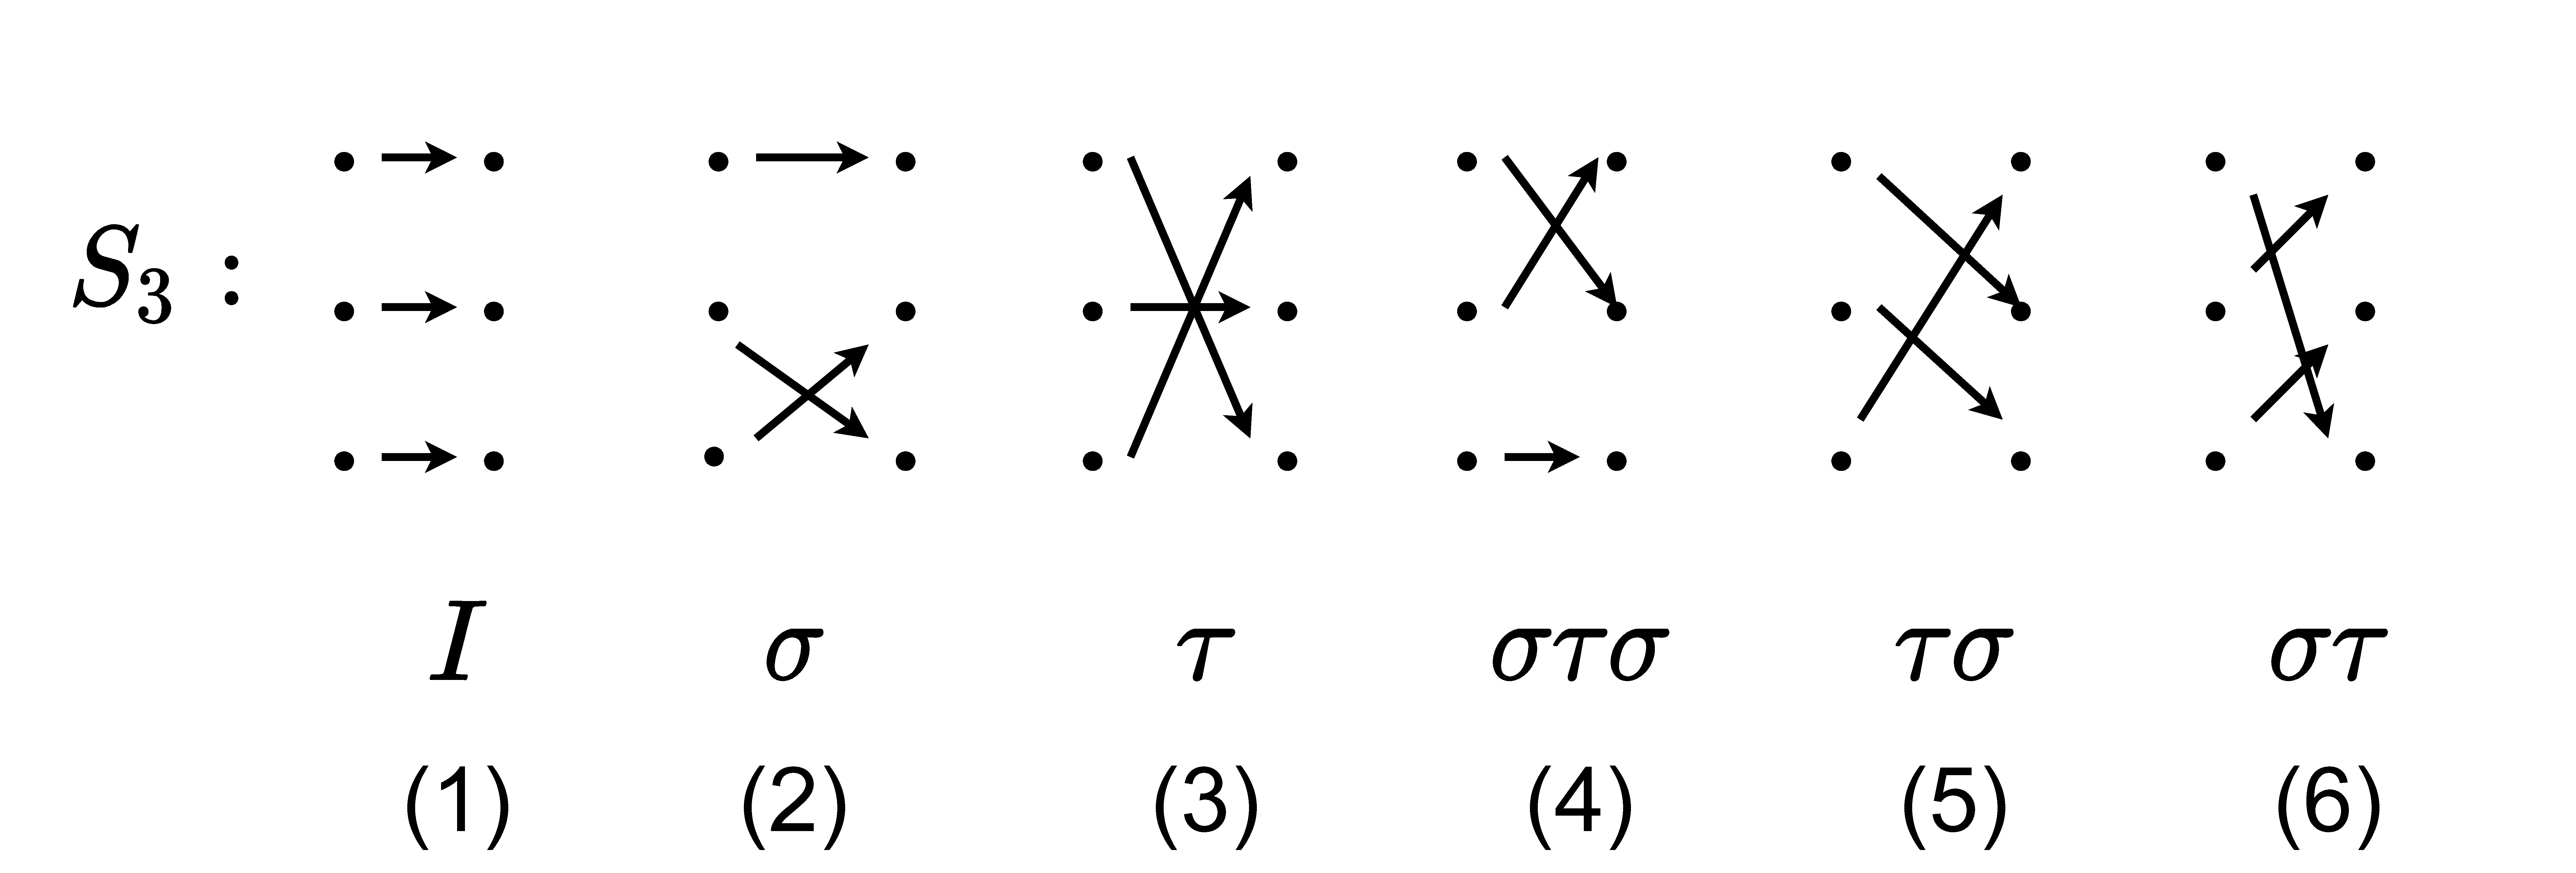
\includegraphics[width=0.8\textwidth]{Figures/S_3 Group Example.pdf}
    \caption{Elements of $S_3$: $S_3$'s group elements correspond to bijective (invertible) mappings from a set of three elements back to itself}
    \label{fig:S3elts}
\end{figure}
\begin{table}[h!]
    \centering
    \begin{tabular}{c||c|c|c|c|c|c|}
         $\bsfrac{b\text{ (right)}}{a\text{ (left)}}$& $I$&$\sigma$&$\tau$&$\sigma\tau$&$\tau\sigma$&$\sigma\tau\sigma$  \\ \hline \hline
         $I$&$I$&$\sigma$&$\tau$&$\sigma\tau$&$\tau\sigma$&$\sigma\tau\sigma$  \\ \hline
         $\sigma$&$\sigma$&$I$&$\sigma\tau$&$\tau$&$\sigma\tau\sigma$& $\tau\sigma$\\ \hline
         $\tau$&$\tau$&$\tau\sigma$&$I$&$\sigma\tau\sigma$ &$\sigma$ &$\sigma\tau$  \\ \hline
         $\sigma\tau$&$\sigma\tau$& $\sigma\tau\sigma$&... & & &$\vdots$ \\ \hline
         $\tau\sigma$ & $\tau \sigma$ &... & & & &   \\ \hline
         $\sigma\tau\sigma$ & $\sigma\tau\sigma$ &... & & & &   \\ \hline
    \end{tabular}
    \caption{Cayley Table for group $S_3$}
    \label{tab:Cayley_S3}
\end{table}
Note that because $\tau\sigma\neq \sigma \tau$ we have a non-abelian group. \steezybreak\\
\noindent The diagram in Figure \ref{fig:S3elts} shows the various bijections that make up the elements of $S_3$, using these mappings we can see some basic facts just by following the points through the composed mappings:
\begin{align}
    \sigma^2&= I \nonumber \\
    \tau^2&=I \nonumber \\
    \sigma\tau\sigma&=\tau\sigma\tau \nonumber
\end{align}
So,
\begin{align}
    \sigma\tau\sigma \circ \tau\sigma = \sigma(\tau\sigma\tau)\sigma= \sigma(\sigma\tau\sigma)\sigma=\sigma^2\tau\sigma^2=I\tau I=\tau \nonumber 
\end{align}
With these facts observed you should be able to fill in the rest of the Cayley table!\steezybreak\\
Now that we have gotten our feet wet with some groups and some ideas relating to their structure, we will prove some elementary facts that hold for all groups. Remember a group is defined by a set $G$ and a group operation $\cdot$ and it obeys four properties.\vspace{-0.5cm}
\section{Some Elementary Results:} 
\begin{lemma}[Elementary Results with Groups]
If $G$ is a group with operation ``$\cdot$", then
\begin{enumerate}[label=\alph*)]
    \item The Identity Element of $G$ is \textit{unique}.
    \item Every elt. in $G$ has a \textit{unique} inverse in $G$
    \item $\forall a \in G$, $(a^{-1})^{-1}=a$
    \item $\forall a,b \in G$, $(ab)^{-1}=b^{-1}a^{-1}$
\end{enumerate}
\textit{Proof:}
\begin{enumerate}[label=\alph*)]
    \item Suppose $e$ and $f$ are both identity elements in $G$, then $f=e\cdot f=e$ (first equality because $e$ is an identity, second equality because $f$ is). $\therefore f=e$ (they are the same).
    \item Suppose $a\in G$ has two inverses $x,y \in G$. Then
    \begin{align}
        x=e\cdot x=(y\cdot a)\cdot x = y\cdot(a\cdot x)=y\cdot e=y\nonumber
    \end{align}
    $\therefore $ inverses $x,y$ are the same elt. (i.e. the inverse of $a$ is unique).\\ 
    \noindent NOTE: part b guarantees if $xy=e$ then you automatically get $yx=e$ since
    \begin{align}
        xy&=e \nonumber \\
        &\implies y\cdot (xy)\cdot y^{-1} = yey^{-1} \nonumber \\
        &\implies yx(y\cdot y^{-1})= yy^{-1} \nonumber \\
        &\implies yxe=e \nonumber \\
        &\implies yx=e \nonumber
    \end{align}
    \item $\forall \ a \in G, (a^{-1})^{-1}=a:$ Take arbitrary $a\in G$, then $a\cdot a^{-1}=e$ and $a^{-1}\cdot a= e$, This set of equations shows that $a$ is the inverse of $a^{-1}$, $\therefore (a^{-1})^{-1}=a$.
    \item $(ab)^{-1}=b^{-1}a^{-1}:$ For all $a,b\in G$ we know $ab\in G$ by closure of group $G$ and furthermore, $ab$ must have a \textit{unique} inverse in $G$, so if $b^{-1}a^{-1}$ satisfies the properties of an inverse for $ab$ then $b^{-1}a^{-1}$ \textbf{is} $(ab)^{-1}$:
    \begin{align}
        (b^{-1}a^{-1})ab= b^{-1}(a^{-1}a)b=b^{-1}eb=b^{-1}b=e \nonumber
    \end{align}
    $\therefore \ b^{-1}a^{-1} \textit{ is the inverse of } ab; \ \ (ab)^{-1}=b^{-1}a^{-1} \ \ \ \ \ \ \ \blacksquare$
\end{enumerate}
\end{lemma}

\begin{tcolorbox}
\begin{center}
    $\star\star\star$ \textbf{Read up to this point to Complete Homework 2 (Located in \ref{sec:HW2})} $\star\star\star$
\end{center}
\end{tcolorbox}
\newpage
\subsection{Laws of Exponents for Groups } This subsection could very well be titled ``Creating new and consistent notation for applying the group operation to a single element with itself many times" because that is what we will be doing here. By unlocking this new notation, that is consistent with our notion of a group, we will be able to prove more nuanced facts with a compact notation.\steezybreak
\begin{definition}[Exponents for Groups]
\noindent $G$ a group, $a\in G$, and $k\in \Z^+$. \\
Exponents on group elements are defined as follows:
\begin{align}
    a^{0} & \eqdef e \nonumber \\
    a^{k} &= a\cdot a\cdot a \cdot ... \cdot a \ (  k \text{ times} )\nonumber \\
    a^{-k} &= a^{-1}\cdot a^{-1} \cdot a^{-1} \cdot ... \cdot a^{-1} \ \ ( k \text{ times}) = (a^{-1})^k\ \  \underset{\star\star}{=} (a^{k})^{-1} \nonumber
\end{align}
\textit{Proof of $\star\star$:} we wish to show that $a^{-k}=(a^{k})^{-1}$ 
\begin{align}
    (a^k)^{-1}=(a\cdot a\cdot a \cdot ... \cdot a)^{-1} = a^{-1}\cdot a^{-1}\cdot a^{-1} \cdot ... \cdot a^{-1}\nonumber 
\end{align}
Where the last equality is established by repeatedly applying part (d) of Lemma 2.3.1. \steezybreak\\
Note also: any power of $e$ is $e$, i.e. $e^{-k}=(e^{-1})^k=e$
\end{definition}

\begin{proposition}[Law of Exponents]
If $G$ is a group, $a\in G, m,n\in \Z$, then 
\begin{align}
    a^m a^n&=a^{m+n} \nonumber \\
    (a^m)^n&= a^{mn} \nonumber
\end{align}
\textit{Proof:} This proof will consider all of the cases for a pair $m,n\in \Z$ and we will show the laws hold for each case.
\begin{enumerate}[label=Case \arabic*:]
    \item $m=0,n=0$, then $m+n=0$ and $mn=0$ and we see:
    \begin{align}
        a^ma^n&=a^0a^0=e\cdot e=e=a^0=a^{m+n} \nonumber \\
        (a^m)^n&=(a^0)^0=e^0=e=a^0=a^{mn} \nonumber
    \end{align}
    \item $m=0, n\neq 0$
    \begin{align}
        a^ma^n&=a^0a^n=e\cdot a^n=a^n=a^{0+n}=a^{m+n} \nonumber \\
        (a^m)^n&=(a^0)^n=e^n=e=a^0=a^{0n}=a^{mn} \nonumber
    \end{align}
    \item $m\neq 0, n=0$ (Proof is Similar to Case (2), leave to students to show)
    \item Both Positive-- $m,n\in \Z^+$ (i.e. both $m$ and $n$ are positive integers)
    \begin{align}
        a^ma^n&=\underset{m\text{ times}}{(a\cdot a\cdot a \cdot ... \cdot a)}\underset{n \text{ times}}{(a\cdot a\cdot a \cdot ... \cdot a)}=a^{m+n} \nonumber \\
        (a^m)^n&=\underset{n\text{ times}}{(a^m\cdot a^m\cdot ... \cdot a^m)}=\underset{n \text{ times}}{(\underset{m }{a\cdot ... \cdot a})...(\underset{m}{a\cdot ... \cdot a})}=a^{mn}\nonumber
    \end{align}
    \item Both Negative-- $m,n\in \Z^+$ (use $-m$ and $-n$) (Note, the square brackets $[\ ]$ used to prove the second statement are normal parentheses, not equivalence class notation, this was just to make the proof read cleaner instead of having a bunch of nested round parentheses)
    \begin{align}
        a^{-m}a^{-n}& \underset{\text{by }\star\star}{=} (a^{-1})^m(a^{-1})^n \underset{\text{by Case (4)}}{=} (a^{-1})^{m+n} \underset{\text{by }\star\star}{=} a^{-(m+n)}=a^{(-m)+(-n)} \nonumber \\
        (a^{-m})^{-n} &\underset{\text{by }\star\star}{=} ((a^m)^{-1})^{-n} \underset{\text{by }\star\star}{=} [((a^m)^{-1})^{-1}]^{n} \underset{\text{Lemma 2.3.1 (c)}}{=} [a^m]^n= a^{mn}= a^{(-m)(-n)} \nonumber 
    \end{align}
    \item Pos-Neg -- $m,n\in \Z^+$ (use $m$ and $-n$)
    \begin{align}
        a^m a^{-n}&\underset{\text{by $\star$}}{=} a^m (a^{-1})^n = \underset{\text{m}}{(a\cdot ... \cdot a)}\cdot \underset{n}{(a^{-1}\cdot ... \cdot a^{-1})} \nonumber
    \end{align}
    Since $a\cdot a^{-1}=e$ we can cancel pairs from the inside out:
    \begin{align}
        &\text{if } m=n, a^m\cdot a^{-n}=e \nonumber \\
        &\text{if } m>n, a^m\cdot a^{-n} \underset{n \ a's\text{ get cancelled}}{=}a^{m-n}=a^{m+(-n)} \nonumber\\
        &\text{if } m<n, a^ma^{-n} \underset{m \ a^{-1} \text{ get cancelled}}{=} (a^{-1})^{n-m} \underset{\text{by $\star$}}{=} a^{-(n-m)}=a^{m+(-n)}\nonumber
    \end{align}
    \begin{align}
        (a^m)^{-n}\underset{\text{by $\star$}}{=} [(a^m)^{-1}]^n\underset{\text{by $\star$}}{=}[(a^{-1})^m]^n \underset{\text{case 4}}{=}(a^{-1})^{mn} \underset{\text{by $\star$}}{=}a^{-mn}=a^{m(-n)}\nonumber
    \end{align}
    \item Neg-Pos -- $m,n\in \Z^+$ (use $-m$ and $n$)\\
    \begin{align}
        a^{-m}a^{n}&\underset{\text{by $\star$}}{=}(a^{-1})^m a^n\underset{\text{Lem 2.3.1 (c)}}{=}(a^{-1})^m[(a^{-1})^{-1}]^n = (a^{-1})^m(a^{-1})^{-n}\underset{\text{by case 6}}{=} (a^{-1})^{m+(-n)} \nonumber \\
        &=(a^-1)^{m-n}= a^{-(m-n)}= a^{(-m)+n} \nonumber \\ \nonumber \\
        (a^{-m})^n&\underset{\text{by $\star$}}{=}((a^m)^{-1})^n\underset{\text{by $\star$}}{=}(a^m)^{-n}\underset{\text{case 6}}{=}a^{m(-n)}=a^{(-m)(n)} \ \ \ \ \ \ \ \ \blacksquare\nonumber
    \end{align} 
\end{enumerate}
Phew, that sure was a lot of cases, but now we can see our bases are covered and these rules for exponents are consistent with our notion of a group and its binary operation ``$\cdot$".
\end{proposition}

\begin{lemma}
$G$ is a group\\
$\forall \ \ a,b,c \in G$,
\begin{enumerate}[label=\roman*)]
    \item if $ab=ac \implies b=c$      (left-cancellation)
    \item if $ba=ca \implies b=c$      (right-cancellation)
\end{enumerate}
%\textit{Note: }These cancellation rules can be very convenient however, we must be careful about what they say and do not say. Remember that, in general, $a\cdot b \neq b\cdot a$ (this is only the case in Abelian groups).\\
\textit{Proof:} 
\begin{enumerate}[label=\roman*)]
    \item Assume $ab=ac$. $a$ is a group element $\therefore \exists \ a^{-1}\in G \ni a^{-1}\cdot a = a\cdot a^{-1}=e$. Now then if we apply this fact to our assumption we see that
    \begin{align}
        a^{-1}ab=a^{-1}ac \implies eb=ec \implies b=c\nonumber
    \end{align}
    \item Assume $ba=ca$,
    \begin{align}
        (ba)a^{-1}=(ca)a^{-1} \implies be=ce \implies b=c \ \ \ \ \ \blacksquare \nonumber
    \end{align}
\end{enumerate}
\end{lemma}
Great! 
\begin{notation}
Writing out the square brackets/boxes $[a],[b], ...$ everywhere to indicate our equivalence classes/group elements is somewhat tiresome. While we would normally denote a group like $\Z_5$ as having elements $\Z_5=\{[0],[1],[2],[3],[4]\}$; By an abuse of notation, we will henceforth describe the equivalence classes with the following more compact notation: $\Z_5=\{0,1,2,3,4\}$. That is, we will intentionally use less precise notation for convenience (so we don't have to put brackets around an equivalence class/group element every time we want to refer to it.)
\end{notation}
\begin{example}
Given $a=\left(\begin{matrix}
4 & 3 \\
0 & 7 
\end{matrix}\right)$ and $b=\left(\begin{matrix}
5 & 0 \\
6 & 7 
\end{matrix}\right)$, $a,b\in GL_2(\Z_9)=\{2\times 2 \text{ matrices with entries in }\Z_9\}$\\
$ab=\left(\begin{matrix}
4 & 3 \\
0 & 7 
\end{matrix}\right)\left(\begin{matrix}
5 & 0 \\
6 & 7 
\end{matrix}\right)\underset{\text{mult. mod 9}}{=}\left(\begin{matrix}
2 & 3 \\
6 & 4 
\end{matrix}\right)$\steezybreak\\
\end{example}
\begin{example}[Constructing a Group from Generators]
\phantomsection
\label{ex:ConstructingFromGenerators}
\index{Constructing a Group from Generators}

\noindent The first problem of our personal group studies (i.e. each student will be assigned a group to study over the remainder of the semester) will be to construct the Cayley table for your group. We will give an example here where we consider the group generated by $a=\left(\begin{matrix}
-1 & -1 \\
0 & 1 
\end{matrix}\right)$ and $b=\left(\begin{matrix}
0 & 1 \\
1 & 0 
\end{matrix}\right)$ under regular matrix multiplication. Under matrix multiplication, 
The approach for constructing a Cayley table from two generating elements $a$ and $b$ is as follows:
\begin{enumerate}
    \item Identify $e$ and put it in the table first
    \item Get powers of $a$
    \item Get powers of $b$
    \item Get products of $a$,$b$ etc.
\end{enumerate}
So we will begin by identifying the identity that works with our $\cdot$ and then we will look at how many unique powers of $a$ exist under the $\cdot$. Then we will do the same for $b$. Lastly we will see if we can make any more elements by multiplying a power of $a$ or $b$ from the left or right by a power of $b$ or $a$, respectively. We start by pointing out the only $2\times 2$ matrix that can work as an identity element under regular matrix multiplication (1) and then we look at how many unique powers of $a$ there are (2):
\begin{align}
    e =\left(\begin{matrix}
1 & 0 \\
0 & 1 
\end{matrix}\right)\nonumber \\
a^2=\left(\begin{matrix}
-1 & -1 \\
1 & 0 
\end{matrix}\right)\left(\begin{matrix}
-1 & -1 \\
1 & 0 
\end{matrix}\right)=\left(\begin{matrix}
0 & 1 \\
-1 & -1 
\end{matrix}\right) \nonumber \\
a^3=a^2\cdot a=\left(\begin{matrix}
1 & 0 \\
0 & 1 
\end{matrix}\right) \nonumber
\end{align}
Continuing on in this fashion let's look at the powers of $b$:
\begin{align}
    b\cdot b= b^2=\left(\begin{matrix}
0 & 1 \\
1 & 0 
\end{matrix}\right)\left(\begin{matrix}
0 & 1 \\
1 & 0 
\end{matrix}\right)=\left(\begin{matrix}
1 & 0 \\
0 & 1 
\end{matrix}\right)=e \nonumber 
\end{align}
So it looks like there is only 1 unique power of $b$, and $b$ is it's own inverse. Let's have a look at the products and see how many unique elements we can come up with in total (so far we have identified four unique elements: $e,a,a^2,b$)
\begin{align}
    a\cdot b &= \left(\begin{matrix}
-1 & -1\\
1& 0 
\end{matrix}\right)\left(\begin{matrix}
0 & 1 \\
1 & 0 
\end{matrix}\right) = \left(\begin{matrix}
-1 & -1 \\
0 & 1
\end{matrix}\right) \nonumber\\
b\cdot a &= \left(\begin{matrix}
0 & 1 \\
1 & 0 
\end{matrix}\right)\left(\begin{matrix}
-1 & -1 \\
1 & 0 
\end{matrix}\right) =\left(\begin{matrix}
1 & 0 \\
-1 & -1 
\end{matrix}\right) = a^2b \ \ \ \ \ \ \text{ (confirm for yourself)} \nonumber \\
b\cdot a^2&= (a^2)^2 b \ \ \ \ \ \ \ \ \ \ \ \ \ \ \ \ \ \ \ \ \ \ \ \ \ \ \ \ \ \ \ \ \ \text{ (confirm for yourself)} \nonumber \\
ba^2b&= (a^2)^2b^2=a\cdot a^3=a \nonumber
\end{align}
From here it should be clear that if we take the product of any one of these elements from the left or right by any other one of the elements we have already discovered, we will just get another element that we have already discovered, i.e., we have identified all of the unique elements. To prove this in the most explicit way possible, we form \textit{each} of those products as the entries of the Cayley table. Let's give each of them a simple name (notice, we named the elements in terms of the powers of the generator elements $a$, $b$ and products of $a$ and $b$) and collect our simplified products (simplified using the relations we discovered above such as $a^3=b^2=e$ and $b\cdot a^2=a\cdot b$) in a Cayley Table.
\begin{table}[ht!]
    \centering
    \begin{tabular}{c||c|c|c|c|c|c|}
         $\bsfrac{b\text{ (right)}}{a\text{ (left)}}$& $e$&$a$&$a^2$&$b$&$ab$&$a^2b$  \\ \hline \hline
         $e$&$e$&$a$&$a^2$&$b$&$ab$&$a^2b$  \\ \hline
         $a$&$a$&$a^2$&$e$&$ab$&$a^2b$& $b$\\ \hline
         $a^2$&$a^2$&$e$&$a$&$a^2b$ &$b$ &$ab$  \\ \hline
         $b$&$b$& $a^2b$&$ab$ &$e$ &$a^2$ &$a$ \\ \hline
         $ab$ & $ab$ &$b$ &$a^2b$ &$a$ &$e$ &$a^2$   \\ \hline
         $a^2b$ & $a^2b$ & $ab$ &$b$ &$a^2$ &$a$ &$e$   \\ \hline
    \end{tabular}
    \caption{\protect{Cayley Table for group generated by $a=\left(\begin{matrix}
-1 & -1 \\
0 & 1 
\end{matrix}\right)$ and $b=\left(\begin{matrix}
0 & 1 \\
1 & 0 
\end{matrix}\right)$ under regular matrix multiplication.}}
    \label{tab:Cayley_from_generators}
\end{table}

Cool, good group, Non-abelian (notice how the Cayley table doesn't have symmetry along diagonal and in general $a\cdot b \neq b\cdot a$) finite group of order 6 (i.e. it has 6 elements). We will discuss the idea of an element "generating" a group under an operation in more detail as we begin to discuss cyclic groups in the next few subsections, don't worry about the definition of a generator yet, the goal right now is just to build some intuition.
\end{example}
\newpage
\section{Subgroups}
\begin{definition}[Subgroups]
$G$ is a group, with $\emptyset \neq H \subset G$. $H$ is a \textit{subgroup} of $G$, denoted $H < G$, if $H$ is itself a group under the operation $\cdot$ in $G$.
\end{definition}

\begin{example} 
$\Z\subset \R \text{ and }\R\text{ is a group under real number ``+"}$\\
$\Z \text{ is also a group under real number ``+", therefore } \Z < \R$
\end{example}
\begin{lemma}[(Used in HW\# 3)]
$G$ is a group with $\emptyset\neq H\subset G$, \\
\begin{align}
    H<G \iff \text{i)}& \ a,b\in H \implies ab\in H \nonumber\text{, and}\\
             \text{ii)}& \ a\in H \implies a^{-1}\in H. \nonumber 
\end{align}
i.e. these two properties are necessary and sufficient for $H<G$.\\
\textit{Proof:} \\
\noindent $\Rightarrow:$ Assume $H<G$, then $H$ is a group so closure and inverse properties hold.\steezybreak\\
\noindent $\Leftarrow:$ Assume closure and inverse properties hold in $H$, it remains to show that $H$ has the associative property and that $H$ has an identity element.\steezybreak\\
\noindent Associativity in $H$ is ``inherited" from $G$: $\forall x,y,z \in H, x(yz)=(xy)z$ because $H\subset G$ so $x,y,z$ are also in $G$ which is associative.\steezybreak\\
\noindent Now we will show $e\in G$ is actually in $H$ too! Take $h\in H$, part ii) of the hypothesis says $h^{-1}\in H$, part i) says that $h\cdot h^{-1}\in H$, but $h\cdot h^{-1}=e$, so $e\in H$. $\blacksquare$
\end{lemma}

\begin{lemma}
$G$ is a group with $\emptyset\neq H\subset G$, and $H$ is finite. Then
\begin{align}
    H<G \iff a,b\in H \implies ab\in H \ \ \ (\text{Closure is satisfied})\nonumber
\end{align}
\textit{Proof:}\\
$\Rightarrow :$ if $H$ is a subgroup then it is a group, so of course it is closed.\\
$\Leftarrow :$ Assume closure in $H$. By Lemma 2.4.1 we only need to show inverse property holds for $H$. (We will first find a way to express $e$):\\ 
\noindent Take $h\in H$, closure in $H$ guarantees that these elements are in $H$:
\begin{align}
    h,h^2,h^3,h^4,...\nonumber
\end{align}
$H$ is finite so the list has repeats, say $h^s=h^r$ for some $s,r\in \Z^+ \text{ with } 0<s<r$. Multiply both sides by $(h^s)^{-1}$ (which is in $G$, since $G$ is a group an contains inverses):
\begin{align}
    e=h^rh^{-s}=h^{r-s} \nonumber
\end{align}
Now, $r-s$ is $>0$, so $h^{r-s}$ is in the list, $\therefore e\in H$. In this list of powers of $h$ we see $e$ shows up as at least two distinct powers of $h$ (all of which are in $H$ by closure), we have $e=h^0,h,h^2,...,h^{r-s-1},h^{r-s}=e$ so $h^{r-s-1}\in H$ too and we claim that this is the inverse of $h$. We can prove this by showing $h^{r-s-1}$ satisfies the inverse property since inverses are unique.
\begin{align}
    h^{r-s-1}\cdot h= h^{r-s-1+1}=h^{r-s}=e \nonumber
\end{align}
so by uniqueness of inverses, Lemma 2.3.1 (b), $h^{r-s-1}$ IS $h^{-1}$, $\therefore h^{-1}\in H$ so by Lemma 2.4.1 $\implies H<G. \ \ \blacksquare$
\end{lemma}

\begin{example}
Every group $G$ has two \textit{trivial subgroups}:
\begin{align}
    G&<G   \ \ ; \ \ \ \ \ \ \ \text{and} \nonumber\\
    \{e\}&<G \ . \nonumber
\end{align}
The rest of the subgroups, if there are any, are the \textit{non-trivial subgroups}.
\end{example}

\begin{example}
Suppose $n\in \Z$, show that $n\Z<\Z$ (thinking of $\Z$ as a group under ``+")\\
\begin{align}
    n\Z&=\{...,-3n,-2n,-n,0,n,2n,3n,...\}\nonumber\\
    &=\{\text{integer multiples of }n\}\nonumber
\end{align}
\textit{Proof:} We need to show closure property and inverse property for $n\Z$. (Note: $n\Z\subset \Z$ and $n\Z\neq \emptyset$ so Lemma 2.4.1 applies)
\begin{enumerate}[label=\roman*)]
    \item Take $an,bn\in n\Z$, $an+bn=(a+b)n$ and $a+b\in \Z$, $\therefore an+bn\in n\Z$, so $n\Z$ is closed under ``+"
    \item For any element in $an\in n\Z$ we can produce an inverse for it under addition like so:
    \begin{align}
        &(an)^{-1} \text{ is } (-a)n\in n\Z. \nonumber \\
        &(an)^{-1}+an=0=e\in \Z \nonumber \\
        &(-an)+an=0=e\nonumber
    \end{align}
    $\therefore n\Z$ is closed under inverses (inverse property holds).\\
    \noindent$\therefore$ by Lemma 2.4.1 $n\Z<\Z \ \ \ \ \blacksquare$
\end{enumerate}
\end{example}

\begin{example}
If $H,K<G$, then $H\cap K < G$.\\
\textit{Proof:} $H\cap K\subset G$ and $H\cap K\neq \{\}$ since both $H$ and $K$ at least contain $e$, perhaps more.\steezybreak\\
\noindent If $a,b\in H\cap K$, then
\begin{align}
    a,b\in H \implies ab\in H \nonumber \\
    a,b\in K \implies ab\in K \nonumber
\end{align}
the two of these implication together implies that $ab\in H\cap K$, $\therefore$ closure holds. Now to show inverses exists in the intersection too. Let $a\in H\cap K$,
\begin{align}
    a\in H \implies a^{-1}\in H \nonumber \\
    a\in K \implies a^{-1}\in K \nonumber
\end{align}
These two implication together imply that $a^{-1}\in H\cap K$ so $H\cap K$ has an inverse for each of it's elements. $\therefore$ by Lemma 2.4.1 $H\cap K < G. \ \ \ \blacksquare$
\end{example}

\begin{example}
Fix $n\in \Z^+$.
\begin{align}
    SL_n(\R)&=\{ n\times n \text{ matrices with entries}\in \R \text{ and determinant }1\} \nonumber \\
    SL_n(\R)&\subset GL_n(\R)=\{\text{invertible }n\times n\text{ matrices with entries in } \R\}\nonumber
\end{align}
$SL_n(\R)$ is the "Special Linear Group of degree $n$ with entries in $\R$".\\
\noindent Prove: $SL_n(\R)<GL_n(\R)$.\\
\textit{Proof:}\\
\noindent $SL_n(\R)$ is non empty since it contains $I_n=\begin{pmatrix}
1 &  &\0 \\
 & \ddots &  \\
\0&&1
\end{pmatrix}$ so Lemma 2.4.1 again applies ($SL_n(\R)$ has infinite elements, actually, this can be easily seen since any invertible $n\times n$ matrix $A$ can generate a member of $S$ by taking $A_{S}=\text{sgn}(\det(P))\ P$  where  $P=\left(\frac{1}{|\det(A)|^{\frac{1}{n}}}\right) A \ \ \ $ and $\text{sgn}(a)$ is defined as $-1$ for $a<0$, $1$ for $a>0$ and is not defined for $a=0$).\\

\begin{enumerate}
    \item Closure: Take $A,B\in SL_n(\R)$, $AB$ is also an $n\times n$ matrix with entries in $\R$ and furthermore $\det(AB)=\det(A)\cdot \det(B)=1\cdot 1=1$ so $AB\in SL_n(\R)$. So $SL_n(\R)$ has closure under matrix mult.
    \item Inverses: $A\in SL_n(\R)\implies \det(A)=1$, $\det(A)\neq 0 \implies A^{-1}$ exists (linear algebra fact). $A^{-1}$ is also an $n\times n$ with entries in $\R$ and furthermore we have $\det(A^{-1})=\det(A)^{-1}=\frac{1}{\det(A)}=\frac{1}{1}=1$\\
     $\therefore A^{-1}\in SL_n(\R)$\\
     \noindent $\therefore$ by Lemma 2.4.1 $SL_n(\R)<GL_n(\R). \ \ \ \blacksquare$
\end{enumerate}
\end{example}

\begin{definition}[Order of an Element]
$G$ group, $a\in G$. The \textit{order} of $a$, denoted $o(a)$ is the smallest positive integer $m$ such that $a^m=e$.\steezybreak\\ that is,
\begin{align}
    a,a^2,a^3, ..., \underset{\text{first time}}{a^m=e}\nonumber
\end{align}
\end{definition}
Being slightly less formal about the above definition we could say "the order of element $a\in G$, written $o(a)$, is the \textit{first} positive (i.e. $m>0$) power of $a$ that equals the identity element $e$".
\begin{example}
$G=\Z$ under "+", what is the order of 1?
\begin{align}
    1^1&=1\nonumber\\
    1^2&=1\cdot 1= 1+1=2\nonumber\\
    1^3&=1\cdot 1\cdot 1=1+1+1=3\nonumber\\
    &\vdots \nonumber \\
    1^m&=1+1+....+1=m \neq 0\nonumber
\end{align}
It's clear we will never get zero. In this scenario, where we cannot pin down the order of the element to a fixed integer $m$, we say that the order of the element is infinite. So order of 1 (in the group $\Z$ under +) is infinite!
\end{example}
As we have just seen it is possible for the order of an element to be infinite. However, if $G$ is a finite group, the order of any element in the group is finite. We can see this using an argument that should be familiar (this argument was used in proof of Lemma 2.4.2):
\begin{align}
    a,a^2,a^3,... \in G \nonumber\\
    G \text{ finite} &\implies a^r=a^s \text{ for some }r,s\in \Z \text{ with }0<s<r \nonumber \\
    &\implies a^r\cdot a^{-s}=a^{s-s} \nonumber \\
    &\implies a^{r-s}=e \nonumber
\end{align}
So, it happens that some positive power of $a$ is $e$ and there has to be a first time that it occurs (first time defines the order of $a$, $o(a)$.)
%\newpage
\begin{example}
Consider the set $G=\{1,2,3,4,5,6\}$ under multiplication $\mod 7$.
\begin{table}[h!]
    \centering
    \begin{tabular}{c||c|c|c|c|c|c|}
         $\bsfrac{b\text{ (right)}}{a\text{ (left)}}$& $1$&$2$&$3$&$4$&$5$&$6$  \\ \hline \hline
         $1$&$1$&$2$&$3$&$4$&$5$&$6$  \\ \hline
         $2$&$2$&$4$&$6$&$1$&$3$& $5$\\ \hline
         $3$&$3$&$6$&$2$&$5$ &$1$ &$4$  \\ \hline
         $4$&$4$&$1$&$5$ &$2$ &$6$ &$3$ \\ \hline
         $5$&$5$&$3$ &$1$ &$6$ &$4$ &$2$   \\ \hline
         $6$&$6$&$5$ &$4$ &$3$ &$2$ &$1$   \\ \hline
    \end{tabular}
    \caption{Cayley Table for group generated by $G={1,2,3,4,5,6}$ under multiply $\mod 7$.}
    \label{tab:Cayley_G_7}
\end{table}

\noindent Symmetry along the main diagonal in this Cayley Table indicates that this group is Abelian. So this is an Abelian Group of order 6. \steezybreak\\
\noindent Now then, to explore this group a little more we would like to \textit{Find the order of each element in $G$}:
\begin{align}
    e^1=e \ \ \ \text{ order of identity is always 1 in every group. So,}  \nonumber \\
    o(1)&=1  \nonumber \\
    2\cdot 2= 4, \ 4\cdot 2= 1 \implies o(2)&=3 \nonumber \\
    3\cdot 3= 2, \ 2\cdot 3= 6, \ 6\cdot 3=4,\ 4\cdot 3= 5,\ 5\cdot 3= 1,\ \implies  o(3)&=6 \nonumber \\
    4\cdot 4= 2,\ 2\cdot 4= 1, \ \implies o(4)&=3 \nonumber \\
    5\cdot 5= 4, \ 4\cdot 5= 6, \ 6\cdot 5=2,\ 2\cdot 5= 3,\ 3\cdot 5= 1, \implies o(5)&=6 \nonumber \\
    6\cdot 6 = 1 \implies o(6)&=2  \nonumber
\end{align}
In table \ref{tab:order_occur} we list the orders that showed up in the top row, and the occurrence of the unique orders (i.e. the number of elements that had this order). Notice that the order of each of the elements is a divisor of the order of $G$, $o(G)=6$.  
% Table listing the divisors of 6 (order of the group) and the occurrence of that divisor as order of one of the elements a \in G. (Working up to Lagrange's Thm looking at finite Cyclic Groups and Subgroups.)
\begin{table}[h!]
    \centering
    \begin{tabular}{|c|c|c|c|c|}\hline
         Order&1&2&3&6   \\ \hline
         No. Elts. of Order& 1&1&2&2 \\ \hline
    \end{tabular}
    \caption{Listing Occurrence of various orders for elements in $G$}
    \label{tab:order_occur}
\end{table}
\end{example}
\steezybreak
\begin{tcolorbox}
\begin{center}
    $\star\star\star$ \textbf{Read up to this point to Complete Homework 3 (Located in \ref{sec:HW3})} $\star\star\star$
\end{center}
\end{tcolorbox}
\steezybreak
\newpage
\noindent Later we will prove this important fact for finite $G$:
\begin{align}
    \forall a \in G, o(a)|o(G) \nonumber
\end{align}
Let's take a shortcut assuming we can use this fact. In the example above, $o(G)=6$, given $o(a)|o(G)$ we would know from the beginning the possible orders are $1,2,3,6$. Consider $3$ from the example before who had element order $o(3)=6$. When we were finding the order of element $3$, just from taking powers of 3 we seemed to cycle through every element before finally finding the identity. We now present a definition 
\begin{definition}[Cyclic Group]
A group $G$ is \textit{cyclic} $\iff$ $\exists \ x\in G \ni G=\{x^n|n\in \Z\}$. Then $x$ is said to \textit{generate} $G$, denoted $G=\langle x \rangle$
\end{definition}
The above notation $G=\langle x \rangle$ could also be read as ``$G$ is cyclic, generated by $x$". \steezybreak\\
In the example, $G=\langle 3 \rangle=\langle 5 \rangle$ since the powers of either these elements, $5$ or $3$, give all elements of $G$.

% Generating Subgroups.
\subsection{Generating Subgroups}
\begin{definition}[Cyclic Subgroup]
$G$ group:
\begin{align}
    \forall \ a\in G, \ \langle a \rangle \underset{\text{def}}{=} \{a^n |n\in \Z\}\nonumber
\end{align}
$\langle a \rangle$ is called the \textit{cyclic subgroup of }$G$ \textit{generated by} $a$.\steezybreak\\
\end{definition}
To verify that $\langle a \rangle$ is a subgroup of $G$ ($\langle a \rangle<G$) we will use Lemma 2.4.1. \\ 
First we note that $\langle a \rangle\neq \emptyset, \ \because \ a^0=e\in \langle a \rangle$, so Lemma 2.4.1 applies.\\
\textit{Proof that $\langle a \rangle < G$:}\\
\textit{Closure:} 
\begin{align}
    a^n,a^m\in \langle a \rangle \implies a^n\cdot a^m=a^{n+m}\in \langle a \rangle \nonumber\\
    \therefore \langle a \rangle \text{ is closed.}\nonumber
\end{align}
\textit{Inverses:} 
\begin{align}
    a^n\in \langle a \rangle \implies (a^n)^{-1}\in G \nonumber\\
    \text{ and }(a^n)^{-1}=a^{-n}, \text{ since } -n\in \Z \implies a^{-n}\in \langle a \rangle \nonumber\\
    \therefore \langle a \rangle \text{ has inverses.} \nonumber
\end{align}
$\therefore$ by Lemma 2.4.1 $\langle a \rangle < G$. $\blacksquare$. \steezybreak \\ 
The reader should note that a cyclic subgroup can always be generated from any element $a\in G$ in this way, \textit{regardless} of whether $G$ is cyclic (Notice, in Defn 2.4.4, and our proof that $\langle a \rangle$ is a subgroup, we only required/assumed $G$ be a group, not a cyclic group). However, the subgroup $\langle a \rangle$ itself, is (very) obviously a cyclic group because there exists an element whose integer powers generate the group, namely, $a$.
\begin{definition}[Subgroup Generated by $W$]
$G$ group, $\emptyset\neq W=\{a_1,...,a_n\}\subseteq G$, the \textit{subgroup of} $G$ \textit{generated by} $W$, denoted:
\begin{align}
    \langle a_1,...,a_n \rangle \nonumber
\end{align}
is the set consisting of these elements:
\begin{itemize}
    \item Integer powers of $a_i, \forall \ i, \ 1\leq i \leq n$ 
    \item All products $a_i^r a_j^s, \ \ 1\leq i,j \leq n \ \ r,s\in \Z$
    \item All products $a_{i_1}^{r_1} ... a_{i_k}^{r_k}, $ where $\{i_1,...,i_k\}\subseteq \{1,...,n\}$ and $r_1,...,r_k\in \Z$.
\end{itemize}

\end{definition}
%
\subsubsection{Problem:} Find all subgroups of $G=\{1,2,3,4,5,6\}$ under $\times_{\mod 7}$\\
Before, we had discovered the following orders for the elements of this group:
\begin{align}
    o(1)&=1, \ o(2)=3 \nonumber \\
    o(3)&=6, \ o(4)=3 \nonumber \\
    o(5)&=6, \ o(6)=2 \nonumber 
\end{align}
\textit{Step 0,} Trivial Subgroups: $\langle 1 \rangle , G$.\\
\textit{Step 1,} Cyclic Subgroups built from one generator: 
\begin{align}
    \langle 1 \rangle &= \{1\} \nonumber \\
    \langle 2 \rangle &= \{2,4,1\} \nonumber \\
    \langle 3 \rangle &= G \nonumber \\
    \langle 4 \rangle &= \{4,2,1\}  \ \ \ \ \ \ \ \text{Note that $\langle 2 \rangle=\langle 4 \rangle$.}\nonumber \\
    \langle 5 \rangle &= G \nonumber \\
    \langle 6 \rangle &= \{6,1\} \nonumber
\end{align}
\textit{Step 2,} Subgroups built from 2 generators:\\
First, notice that $\langle e, \text{any other element } z\rangle = \langle z\rangle$ since $e$ generates nothing but $e$. So $\langle 1, z\rangle$ is covered in step 1 $\forall z\in G$.
\begin{align}
    \langle 2,3 \rangle &= G \ \ \text{ because } 3 \text{ generates everything} \nonumber \\
    \langle 2,4 \rangle &= \{2,4,1\} \ \ \text{ Nothing new here} \nonumber \\
    \langle 2,5 \rangle &= G \nonumber \\
    \langle 2,6 \rangle &= \{2,4,1,6,5,3\}= G  \nonumber \\
    \langle 3,4 \rangle &= G \nonumber \\
    \langle 3,5 \rangle &= G \nonumber \\
    \langle 3,6 \rangle &= G \nonumber \\
    \langle 4,5 \rangle &= G \nonumber \\
    \langle 4,6 \rangle &= \{2,4,1,6,5,3\}= G \nonumber \\
    \langle 5,6 \rangle &= G \nonumber 
\end{align}
\textit{Step 3,} Subgroups built from 3 generators:\\
First note that if $\langle x,y\rangle=G$, then $\langle x,y,z \rangle=G$.\\
Since $\langle 2,4\rangle\neq G$, we consider $\langle 2,4,z \rangle$
\begin{align}
    \langle 2,4,3 \rangle &=G \nonumber \\
    \langle 2,4,5 \rangle &=G \nonumber \\
    \langle 2,4,6 \rangle &=G \nonumber 
\end{align}
All trios give $G$ so we don't need to consider quadruples or anything further. We can display the subgroup organization with what is known as a \textit{subgroup lattice}:
\begin{figure}[h!]
    \centering
    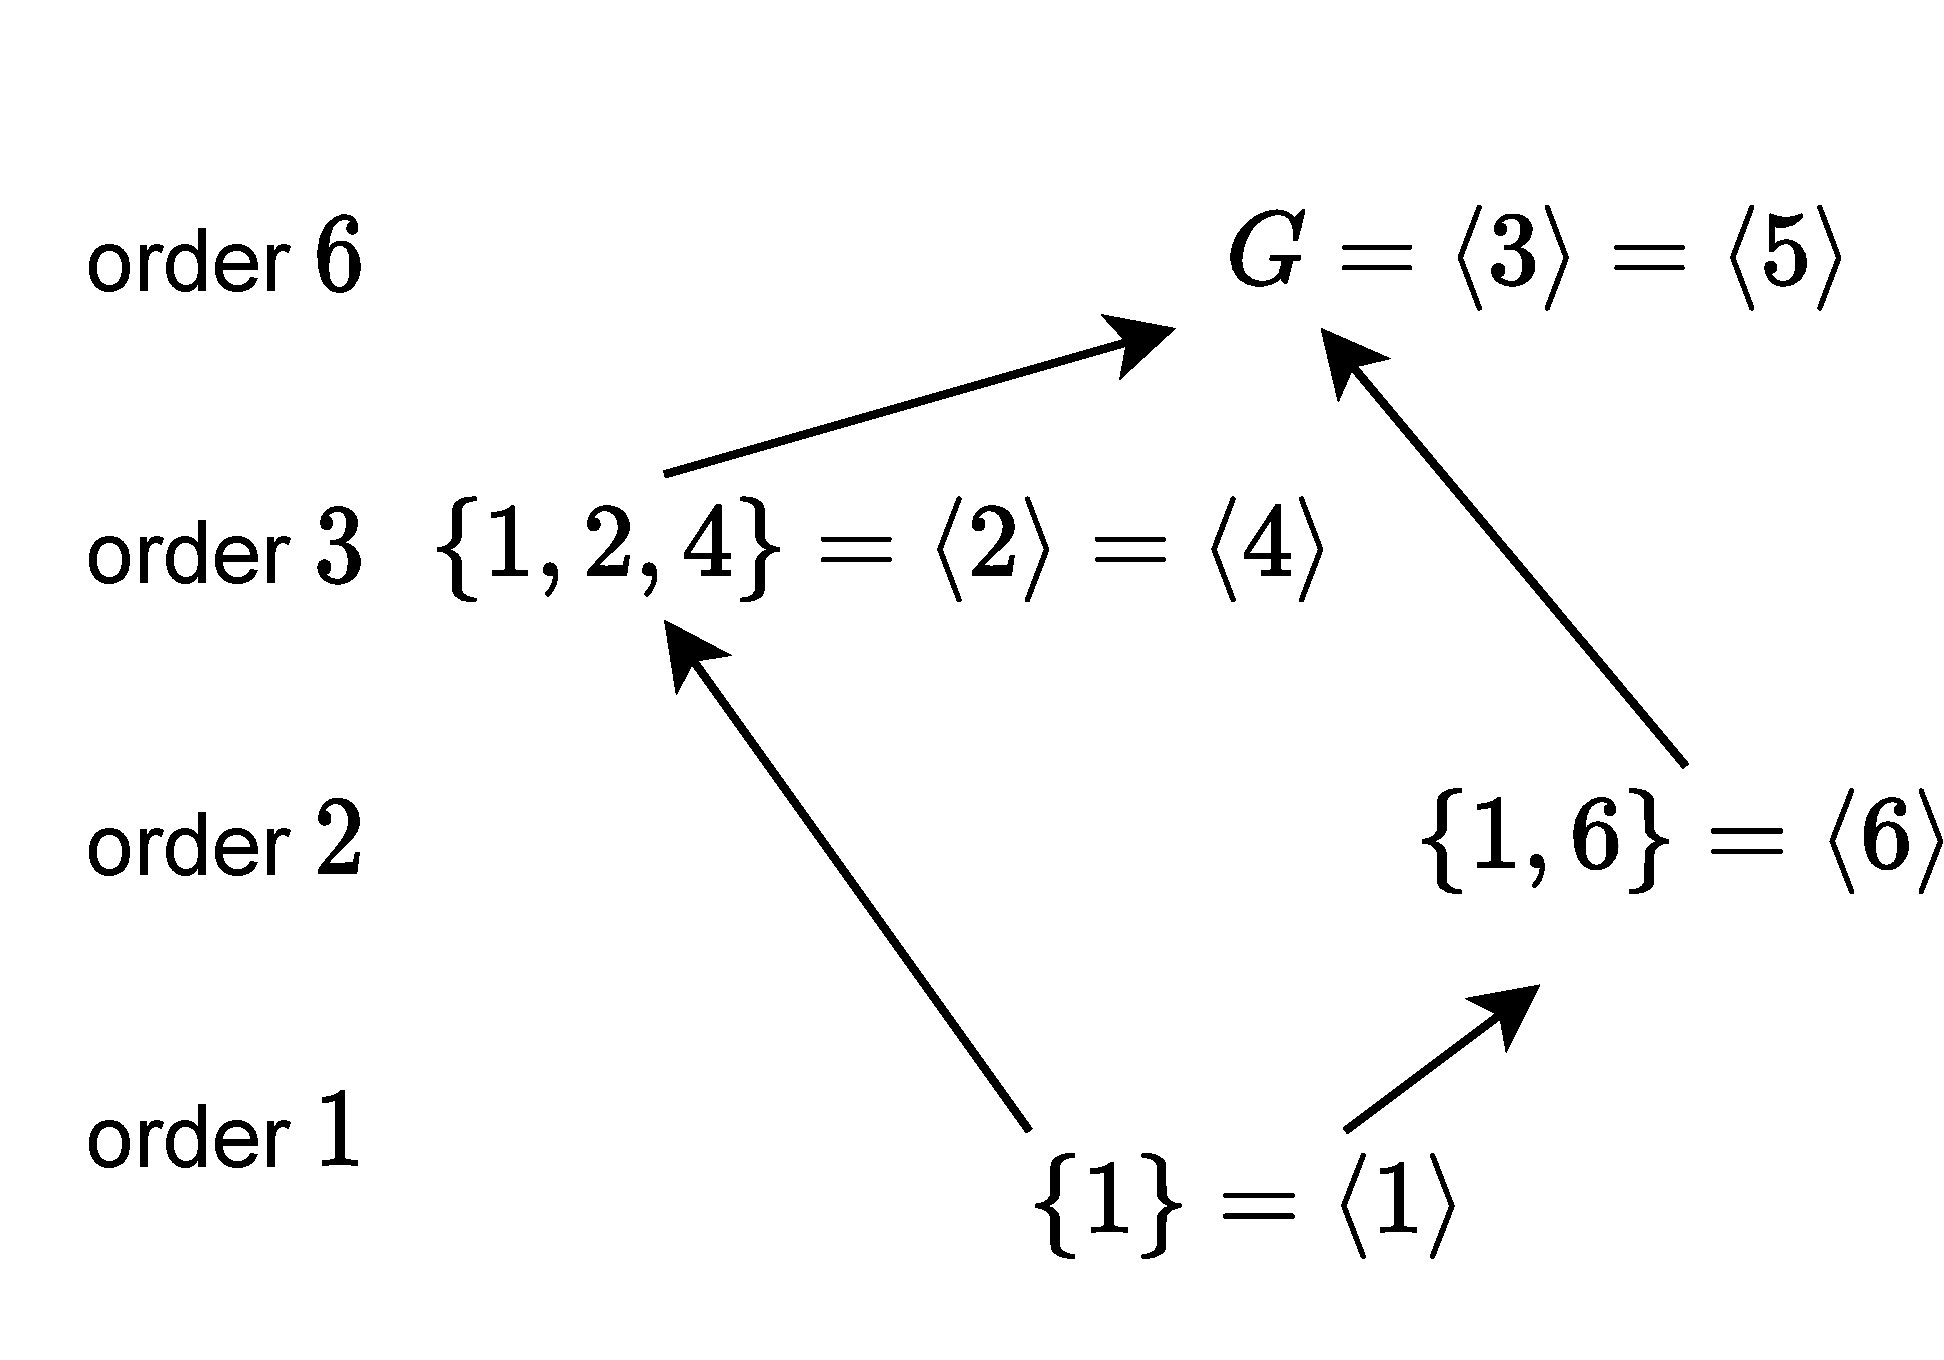
\includegraphics[width=0.5\textwidth]{Figures/Subgroup Lattice example.pdf}
    \caption{Subgroup Lattice for $G=\{1,2,3,4,5,6\}$ under multiplication $\mod 7$. Objects in this lattice are the subgroups of $G$, Arrows in this diagram correspond to the \textit{partial order} of set inclusion, where an arrow exists from $A\rightarrow B \iff A\subset B$}
    \label{fig:Subgroup_lattice}
\end{figure}
\newpage
\begin{proposition}[a.k.a Prop $\clubsuit$ (or \#27 from pg. 47 in Herstein)]
Every subgroup of a cyclic group is cyclic.\\
\textit{Proof:} Assume $G$ is cyclic with generator $a$, $a\in G$.
\begin{align}
    G=\langle a\rangle= \{a^n|n\in \Z\} \nonumber
\end{align}
\begin{enumerate}
    \item The trivial subgroup, $e$, is cyclic.
    \item Suppose that $H<G$ is a non-trivial subgroup of $G$  ($H\neq \{e\}$), then $\exists x\in H, x\neq e$ and since $H<G \implies x^{-1}\in H$.
    \begin{align}
        x\in G \implies \exists \ k \in \Z \ni x&=a^k \ \ \text{ and so,} \nonumber \\
        x^{-1}&=(a^k)^{-1}=a^{-k} \nonumber
    \end{align}
    Since either $k$ or $-k$ is positive, $H$ contains at least one positive power of $a$.\\
    Consider the smallest positive integer $n$ such that $a^n\in H$.\\
    \textit{Claim:} $H=\langle a^n \rangle $.\\
    \textit{Proof:} We must show $H\subset \langle a^n \rangle$ and $ \langle a^n \rangle \subset H$ we begin with the latter of the containments.\\
    $\langle a^n \rangle \subset H:$ Since $a^n\in H$, and $H$ is closed and contains inverses of all its elements, $(a^n)^j\in H \ \forall \ j\in \Z$. $\therefore \langle a^n \rangle \subset H$.\steezybreak\\
    $ H\subset\langle a^n \rangle :$ Take $h\in H$. $h\in G \implies \exists m\in\Z \ni h=a^m$. Next, we will use the euclidean algorithm to "divide" (we use quotes because $r$ may not equal $0$, "divide" in the grade school sense) $m$ by $n$.
    \begin{align}
        &\text{Eucl. Alg. } \implies \ \exists \ q,r\in \Z \ni \ m=qn+r, \ \ \text{ where } 0\leq r < n \nonumber \\
        &\text{then  }h=a^m=a^{qn+r}=(a^n)^q a^r \ \ \ \ (\text{Idea: show }r=0)\nonumber
    \end{align}
    Note that $(a^n)^q \in H \text{ by closure since } a^n \in H \implies [(a^n)^q]^{-1}\in H$. Therefore we can see $a^r$ is a member by closure
    \begin{align}
        a^r=[(a^n)^q]^{-1}\cdot h, \ \ \therefore a^r\in H \nonumber
    \end{align}
    Now we note again that $0\leq r < n$, $n$ is the \textit{smallest} positive integer $\ni a^n\in H \implies r$ can't be positive otherwise the definition of $n$ is violated. $\therefore r=0$.
    \begin{align}
        &\therefore \ h= (a^n)^q\cdot a^0 = a^{nq}\in \langle a^n \rangle \nonumber \\
        &\therefore H\subset \langle a^n \rangle \nonumber
    \end{align}
\end{enumerate}
\indent $\ \ \ \ \ \ \ \ \ \ \therefore H=\langle a^n \rangle.  \ \ \ \ \ \ \ \ \blacksquare$
\end{proposition}

\begin{definition}[Congruence mod $H$]
$H<G$, $G$ is a group. For $a,b\in G$, a is congruent to $b\mod H$, denoted
\begin{align}
    a\equiv b \mod H \iff ab^{-1}\in H \nonumber
    \end{align}
\end{definition}

\begin{example}
The definition above is the generalization of "congruence mod $n$" in $\Z$. Recall $n\Z \subset \Z$.
\begin{align}
    a\equiv b\mod (n\Z) &\iff ab^{-1}\in n\Z \ \ \ \ \ \text{(abstract notation)}\nonumber \\
     &\iff a-b \in n\Z \ \ \ \ \ \text{(specific to example)}\nonumber \\
     &\iff a-b \text{ is and integer multiple of }n \nonumber \\
     &\iff n|a-b \nonumber \\
     &\iff a\equiv b\mod n \nonumber 
\end{align}
\end{example}
\begin{lemma}
Congruence $\mod H$ is an equivalence relation on $G$.\\
\textit{Proof:}\\
\begin{enumerate}
    \item \textit{Reflexivity:} $\forall a \in G, aa^{-1}=e\in H$ so $a\equiv a \mod H$.
    \item \textit{Symmetry:} if $a\equiv b \mod H \implies ab^{-1}\in H$, $H$ is a subgroup so it must contain $(ab^{-1})^{-1}$.
    \begin{align}
        (ab^{-1})^{-1}=(b^{-1})^{-1}a^{-1}=ba^{-1} \ \ \ \text{ Lemma 2.3.1 } \nonumber \\
        \therefore ba^{-1}\in H \nonumber
    \end{align}
    so symmetry holds.
    \item \textit{Transitivity:} Assume $a\equiv b \mod H$ and $b\equiv c \mod H$ for $a,b,c \in G$. Then,
    \begin{align}
        ab^{-1}\in H \nonumber \\
        bc^{-1}\in H \nonumber \\
        ab^{-1}\cdot bc^{-1}\in H \ \ \ \ \text{ by closure}\nonumber \\
        \implies aec^{-1}\in H \implies ac^{-1}\in H \nonumber
    \end{align}
    therefore $a\equiv c \mod H$, $\equiv \mod H$ is transitive. $\ \ \ \ \blacksquare$
\end{enumerate}
\textit{Notation:} As in the special case where $G=\Z$, $[a]$ denotes the equivalence class (congruence class) of $a$:
\begin{align}
    [a]&=\{x\in G \ | \ a\equiv x\mod H\} \nonumber \\
    &=\{x\in G \ | \ a x^{-1} \in H\} \nonumber
\end{align}
\end{lemma}
\begin{definition}[Cosets]
$H<G$, $a\in G$. Define $Ha=\{ha|h\in H\}$, $Ha$ is called a right coset of $H$ in $G$.\\
(similarly, $aH=\{ah|h\in H\}$ is a left coset.)
\end{definition}
\begin{lemma}
$\forall a\in G, Ha=[a]$.\\
\textit{Proof:}\steezybreak\\
\textit{$Ha\subset [a]$:} \\ 
Take $ha\in Ha$. We need to get $ha\in [a]$.
\begin{align}
    ha\in[a] &\iff a\equiv ha \mod H \nonumber\\
    &\iff a (ha)^{-1} \in H \nonumber
\end{align}
Well let's check what $a(ha)^{-1}$ is.
\begin{align}
    a(ha)^{-1}&= a(a^{-1}h^{-1}) \ \ \ \ \text{By Lemma 2.3.1} \nonumber  \\
              &= (aa^{-1})h^{-1} \nonumber \\
              &= eh^{-1} \nonumber \\
              &= h^{-1} \nonumber 
\end{align}
Since $h\in H$, $h^{-1}\in H$, therefore $ha\in [a]$, and so $H\subset [a]$.\steezybreak\\
\textit{$[a]\subset Ha$:} \\
Take $x\in [a]$. Then $a\equiv x \mod H$ so $ax^{-1}\in H$. $H<G$ so $(ax^{-1})^{-1}\in H \underset{L 2.3.1}{\implies} xa^{-1}\in H$. \\
So $x=x\cdot e=x(a^{-1}a)=(xa^{-1})a\in Ha$. Therefore $H\subset [a]$.\\
$\therefore Ha=[a]$. $\ \ \ \ \ \ \ \blacksquare$
\end{lemma}
\setcounter{dummy_lemma}{3}
\begin{corollary}
If $Ha$ and $Hb$ are right cosets of $H$ in $G$, then either $Ha=Hb$ or $Ha\cap Hb=\emptyset$.\\
\textit{Proof:} This fact follows directly from Lemma 2.4.4 (above) and Thm 1.1.1. Under any equivalence relation, classes are either identical or disjoint. $\blacksquare$
\end{corollary}
Having seen this corollary, we can draw a picture representing $G$ and the various cosets of $G$'s subgroup $H$ like in Figure \ref{fig:cosets_fig}.
\begin{figure}[h!]
    \centering
    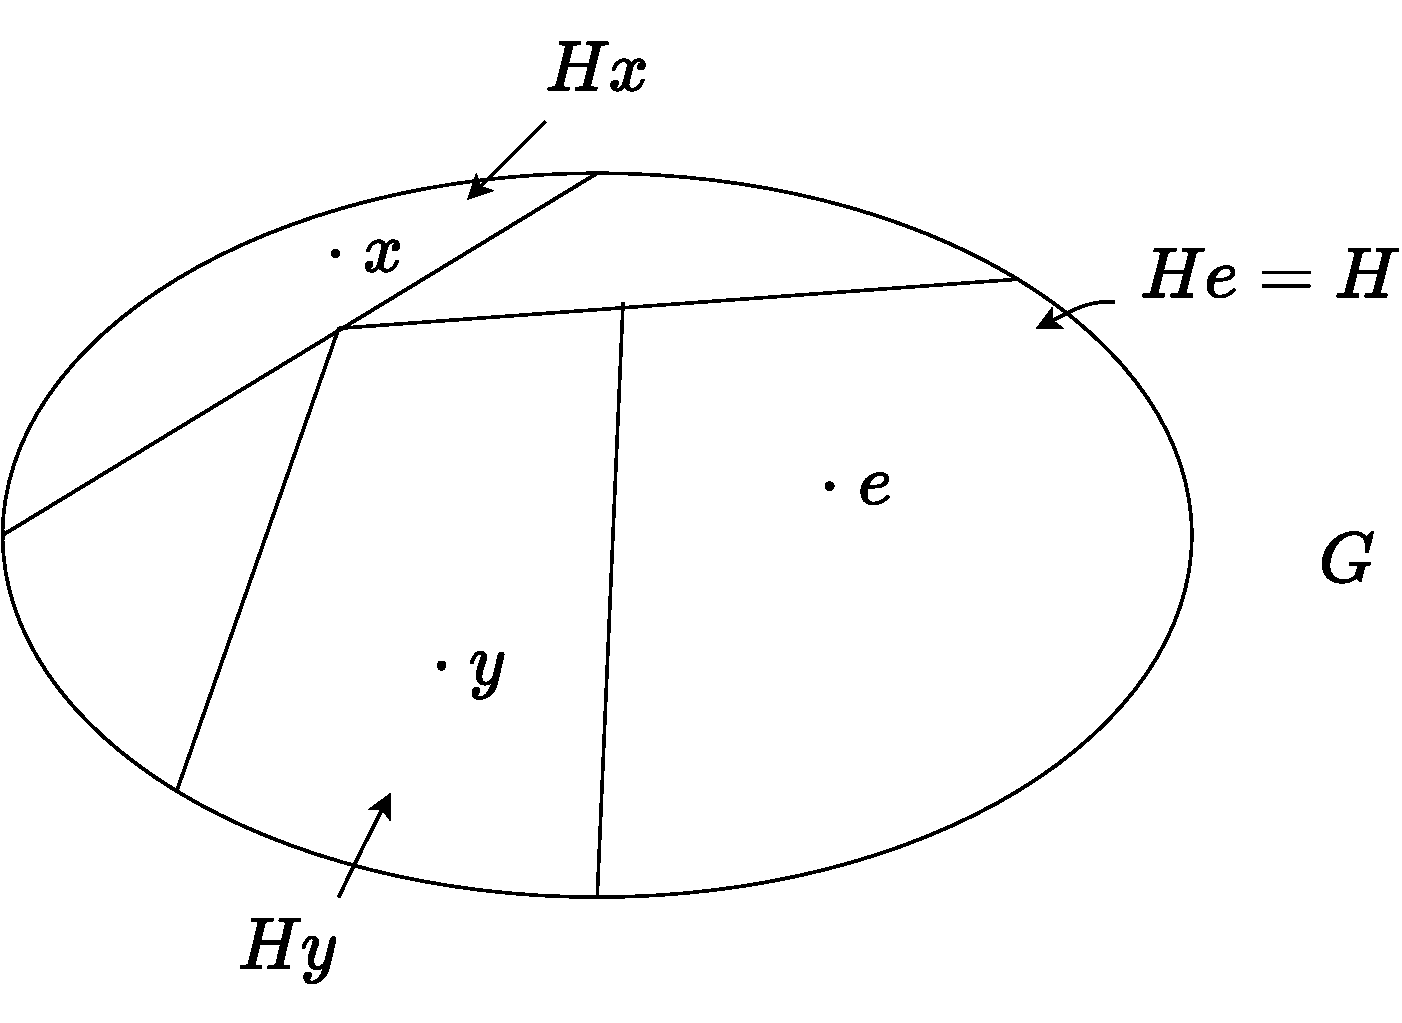
\includegraphics[width=0.6\textwidth]{Figures/Cosets_pic.pdf}
    \caption{Cosets of $H$ in $G$}
    \label{fig:cosets_fig}
\end{figure}
\begin{lemma}
If $Ha$ and $Hb$ are right cosets of $H$ in $G$, there is a bijection (1-1 correspondence) between them.\\
\textit{Proof:}\\
Define $\sigma: Ha\rightarrow Hb$ by
\begin{align}
    \sigma(ha)=hb \nonumber
\end{align}
\textit{$\sigma$ is surjective:} Take $y\in Hb$, then $\exists \ h\in H\ni y=hb$, so $\sigma(ha)=hb=y$. Since $ha$ serves as a preimage for $y$, $\sigma$ is surjective.\\
\textit{$\sigma$ is injective:} Take $x,y \in Ha $, $x\neq y$.
\begin{align}
    x,y &\in Ha \implies \exists \ \ h_1,\ h_2\in H\ni \ h_1a=x, \ \ h_2a=y \nonumber \\
    \sigma(x)&=\sigma(h_1 a)=h_1 b \nonumber \\
    \sigma(y)&=\sigma(h_2 a)=h_2 b \nonumber
\end{align}
Now, if $h_1b=h_2b$, then $b^{-1}\in G \implies h_1=h_2$ but this then implies that $h_1a=h_2a$, but this contradicts $x\neq y, \ \Rightarrow \Leftarrow$! So it must be true that $\sigma(x)\neq \sigma(y)$.\\
$\therefore \ \sigma$ injective. $\blacksquare$ 
\end{lemma}
\setcounter{dummy_lemma}{4}
\begin{corollary}
If $H$ is finite, then all the right cosets of $G$ have the same number of elements, namely $o(H)$.\\
\textit{Proof:} $H$ finite $\implies$ $Ha$ finite $\forall a \in G$, and the bijection from Lemma 2.4.5 guarantees uniform size. Since $H$ is one of the cosets ($He$) the size of each coset is the size of $H$. $\ \ \ \ \ \blacksquare$
\end{corollary} 

\subsection{Lagrange's Theorem (1770)} 
Joseph-Louis Lagrange was an Italian-born mathematician who was naturalized as a French citizen during adulthood. He lived from 1736 until 1813. Lagrange's work in number theory and math analysis had great influence on a young \'Evariste Galois (born 1811). Two of Lagrange's doctoral students include Joseph Fourier and Sim\'eon Poisson.
\setcounter{dummy}{0}
\begin{theorem}[Lagrange's Theorem] \hspace{0.1in}\steezybreak\\
If $G$ is a finite order group and $H<G$, then $o(H)|o(G)$.\steezybreak\\
\textit{Proof:} Suppose $H=\{h_1,...,h_r\}$ where $h_1=e$, so $o(H)=r$. \\
If $H=G$, then $o(G)=r$ so $o(H)|o(G)$.\\
Now let's consider $H\subset G$ with $H\neq G$. Then $\exists \ a\in G\ni a\not \in H$. So far we can find 2 disjoint cosets:
\begin{align}
    H=He&=\{h_1,...,h_r\}  \ \ \ \ \ &\text{note }h_1&=e\nonumber \\
    Ha&=\{h_1a,...,h_ra\} \ \ \ &\text{note }h_1a&=a\nonumber
\end{align}
If this accounts for all of the elements in $G$ then $o(G)=2o(H)$, so $o(H)|o(G)$. Otherwise, $\exists b \in G$, $b\not \in H\cup Ha$, we can use $b$ to build another coset:
\begin{align}
    Hb=\{h_1b,...,h_rb\}\nonumber
\end{align}
disjoint from the previous ones. We can continue in this way, producing cosets different from the previous ones, until $G$ is exhausted ($G$ finite). Eventually we will end up with $k$ (an integer) cosets each with $r$ elements. Then $o(G)=k o(H)$ since $k\in \Z$, $o(H)|o(G)$. $\blacksquare$
\end{theorem}
\begin{definition}[Index of a Subgroup]
for $H<G$, the \textit{index of} $H$ \textit{in} $G$, denoted:
\begin{align}
    i_G(H) &= \text{\# of right cosets of }H \text{ in } G \nonumber \\
    &= \frac{o(G)}{o(H)} \nonumber
\end{align}
is the number of distinct right cosets of $H$ in $G$ ("$k$" in the proof of Lagrange's Thm.)
\end{definition}
We will now present five important corollaries of Lagrange's theorem. Corollary 5 will be proven first as it is parallel to the other 4 corollaries (Cor 5. follows directly from Lagrange and does not require, nor suffice for, Cors 1.- 4.) and then we will prove a chain of corollaries as we have depicted in Figure \ref{fig:Lagrange_corrs}
\begin{figure}[ht!]
    \centering
    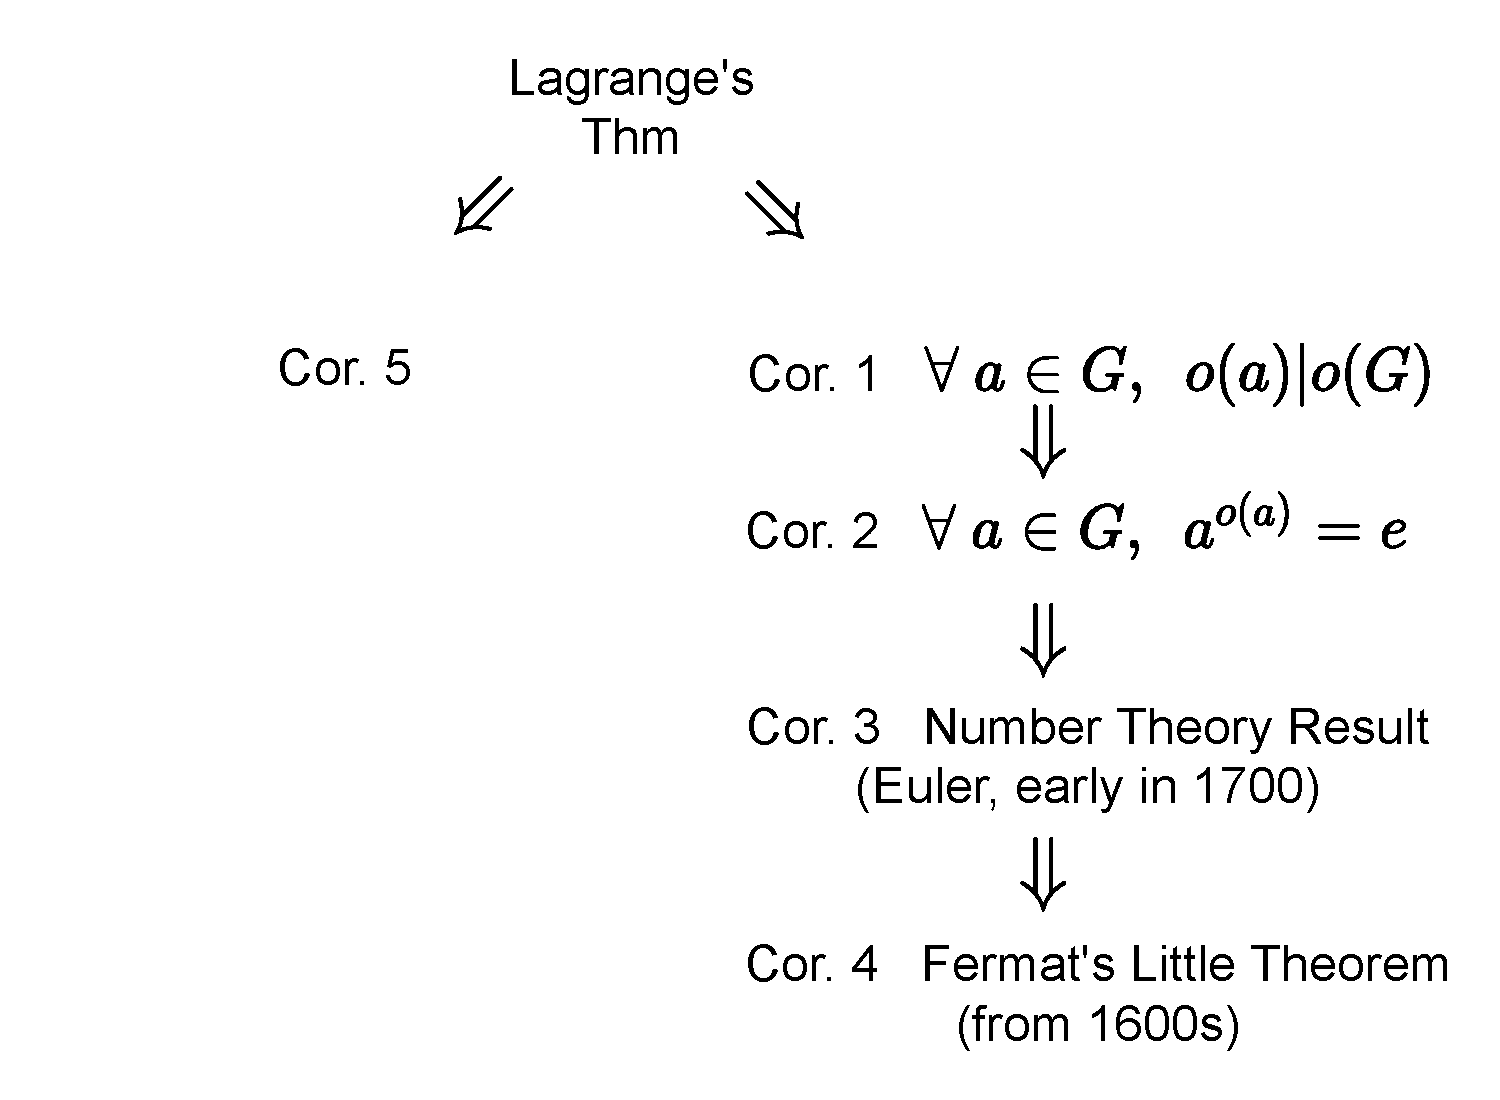
\includegraphics[width=0.6\textwidth]{Figures/Lagrange_corrollaries.pdf}
    \vspace{-0.1in}\caption{Five Corollaries of Lagrange's Theorem}
    \label{fig:Lagrange_corrs}
\end{figure}
\newpage
\setcounter{dummy_lemma}{0}
\begin{corollary}[Lagrange Cor. 5] 
If $G$ is finite, and $o(G)=p$ is prime, then $G$ is cyclic and has no non-trivial subgroups. \\
\textit{Proof:} Say $H<G$, Lagrange says $o(H)|o(G)$, so $o(H)$ can be $1$ or $p$.
\begin{align}
    \text{if }o(H)&=1, \text{ then } H=\{e\}, \text{ trivial.} \ \nonumber\\
    \text{if }o(H)&=p, \text{ then } H=G, \text{ trivial.} \ \nonumber
\end{align}
$o(G)$ prime means $\exists \ a\in G\ni a\neq e$. Consider the subgroup generated by $a$.
\begin{align}
    \langle a \rangle= \{a^n|n\in \Z\}\nonumber
\end{align}
Now, $\langle a \rangle < G \ \implies \langle a \rangle= G$ or $\langle a \rangle =\{e \}$, however since $a$ was non-trivial the second of these possibilities cannot occur.\\
$\therefore \langle a \rangle = G$. $\blacksquare$
\end{corollary}
One should note that when $o(G)$ prime, the proof provided above implies that ANY non-identity $a\in G$ can generate $G$ (In the proof we say we know AT LEAST one must exist because $p$ prime implies $p>1$ but this generating property holds for any $a\in G\ni$  $a\neq e$.)

\setcounter{dummy_lemma}{0}
\begin{corollary}[Lagrange Cor. 1]
$G$ a finite group, then $a\in G \implies o(a)|o(G)$.\\
\textit{Proof:} Say $o(a)=m$ and consider $H=\langle a \rangle =\{e,a^1,a^2,...,a^{m-1}\}$, note $e=a^0=a^m$.\steezybreak\\
Are these all different? Suppose $H$ has a repeat:
\begin{align}
    a^i=a^j \ &\text{ for some } 0\leq i < j \leq m-1 \nonumber \\
    &\implies a^ia^{-i}=a^{j-i} \nonumber \\
    &\iff e=a^{j-i}, \ \text{and } 0<j-i\leq m-1-i < m \nonumber
\end{align}
This is a contradiction of the definition of $o(a)$ (\textit{smallest} positive integer, $m$, power of $a$ such that $a^m=e$) $\Rightarrow \Leftarrow$. So $H$ has $m$ elements ($o(H)=m$).\\
Lagrange $\implies$ $o(H)|o(G) \ \implies o(a)|o(G). \ \  \blacksquare$
\end{corollary}

\setcounter{dummy_lemma}{0}
\begin{corollary}[Lagrange Cor. 2]
$G$ a finite group, with $a\in G$, then it must be true that $a^{o(G)}=e$.\\
\textit{Proof:} Cor 1. $\implies$ $o(a)|o(G) \ \implies \exists \ n\in \Z \ni o(G)=n(o(a))$, now calculate $a^{o(G)}$...
\begin{align}
    a^{o(G)}=a^{n(o(a))}=[a^{o(a)}]^n=[e]^n=e^n=e. \ \ \blacksquare \nonumber
\end{align}
\end{corollary}
Before we present and prove Corollary 3, we need one more definition and we will look at an example of it and a family of groups closely related to this newly defined function.
\begin{definition}[Euler Totient Function (Euler $\phi$-function)]
The Euler $\phi$-function (a.k.a The Euler Totient Function):\\
\begin{align}
    &\phi : \Z^+\rightarrow \Z^+ \ \ \text{ is a mapping from positive integers to positive integers defined as follows:}\nonumber \\
    &\phi(1)=1 \nonumber \\
    &\phi(n)=\text{the number of positive integers }<n\text{ and relatively prime to }n \nonumber
\end{align}
\end{definition}

\begin{example}
What is $\phi(10)$?, to find out, we look at the numbers less than 10 and greater than 0, and throw out any numbers who share factors with 10.
\begin{align}
1,2,3,4,5,6,7,8,9 \nonumber \\
1,\not 2, 3,\not 4, \not 5, \not 6,7,\not 8, 9 \nonumber \\
\underset{1}{1},\not 2, \underset{2}{3},\not 4, \not 5, \not 6,\underset{3}{7},\not 8, \underset{4}{9} \nonumber \\
\therefore \phi(10)=4. \nonumber \\
\text{Also note, for any prime number }p, \ \ \phi(p)=p-1 \nonumber
\end{align}
\end{example}

\begin{example}
For $n\in \Z^+$, define $G_n=\{m\in \Z^+ | m<n \text{ and } GCD(m,n)=1\}$. $G_n$ is a group under multiplication mod $n$. This family of groups is referred to as \textit{"The multiplicative group of integers modulo $n$"}, e.g. 
\begin{align}
    G_{10}= \{1,3,7,9\} \ \text{ under mult. mod }10 \nonumber \\
    G_{7}= \{1,2,3,4,5,6\} \ \text{ under mult. mod }7 \nonumber 
\end{align}
For this family of groups, we have that $o(G_n)=\phi(n)$. Ok we've introduced enough to talk about Cor. 3.
\end{example}

\setcounter{dummy_lemma}{0}
\begin{corollary}[Lagrange Cor. 3 (Euler)]
If $n\in \Z^+$ and $a\in \Z$ with $GCD(a,n)=1$, then $a^{\phi(n)}\equiv 1 \mod n$. \steezybreak\\
\textit{Proof:} We will consider two cases $n=1$ and $n>1$ and show the fact is true under either scenario. \steezybreak\\
If $n=1$, then $\phi(1)=1$ and $\forall a \in \Z$, $GCD(a,1)=1$, also $a\equiv 1 \mod 1$ because $1|(a-1)$.\steezybreak\\
If $n>1$, take any $a\in \Z \ni GCD(a,n)=1$. Euclidean Alg. $\implies \exists \ q,r \in \Z \ni a=qn+r$. Where $0\leq r < n$.\steezybreak\\
\textit{Claim:} $r\in G_n$ (must show $r\neq 0$, $GCD(r,n)=1$). \\
\textit{Proof of Claim: }If $r=0$, then $a=qn$, so $n|a$, and $GCD(a,n)=n\neq 1$ $\Rightarrow\Leftarrow$. So $r$ is a positive integer $<  n$. \steezybreak\\
Say $GCD(r,n)=d$, then $d|r$ and $d|n$, and by observation \#4, $d|a$, a linear combination of $r$ and $n$. Since $d|a$ and $d|n$, $d|GCD(a,n)$. But $GCD(a,n)=1$ by assumption so by observation \#1 about divisions, $\implies d= \pm 1 \implies d= 1$, so $r$ and $n$ are relatively prime $\blacksquare$ (end of proof of supporting claim, Cor. 3 proof continues).\steezybreak\\
Apply Cor \# 2: $G_n$ finite group, $r\in G_n$. $o(G_n)=\phi(n)$, so $r^{\phi(n)}=1$ ($1$ is $e$ in $G_n$).\\
In the language of $\Z$
\begin{align}
    &r^{\phi(n)}\equiv 1 \mod n\nonumber \\
    \text{Now, } a=qn+r &\implies a\equiv r \mod n \nonumber \\
    &\implies a^{\phi(n)} \equiv r^{\phi(n)}\mod n \nonumber \\
    &\therefore \text{ by transitivity of }\equiv \mod n, \ a^{\phi(n)}\equiv 1 \mod n \ \ \ \blacksquare \nonumber 
\end{align}
\end{corollary}

\begin{example}
Reduce $2^{523}\mod 11$.
\begin{align}
    a&=2 \nonumber \\
    n&=11 \ \ \textit{prime} \nonumber \\
    \phi(n)&= 10 \nonumber \\
    \text{Euler Cor. }&\implies 2^{10}\equiv 1 \mod 11 \nonumber \\
    &\implies (2^{10})^{52}\equiv 1^{52}\mod 11 \nonumber \\
    &\implies 2^{520}\equiv 1 \mod 11 \nonumber \\
    2^3&\equiv 2^3\mod 11 \ \ \ (\equiv \mod n \text{ is reflexive})\nonumber \\
    2^{523}&\equiv 1\cdot 2^{3}\mod 11\nonumber \\
    \therefore 2^{523}&\equiv 8 \mod 11 . \nonumber
\end{align}
\end{example}
%\newpage
\setcounter{dummy_lemma}{0}
\begin{corollary}[Lagrange Cor. 4 (Fermat's "Little Theorem")]
$p$ prime and $a\in \Z$, then $a^p\equiv a \mod p$. \\
\textit{Proof:} $p$ prime $\implies \phi(p)=p-1$. Take any $a\in \Z$, then $GCD(a,p)=1$ or $p$. \\
If $GCD(a,p)=1$, then $a$ is relatively prime to $p$
\begin{align}
    \implies &a^{p-1}\equiv 1\mod p \ \ \text{ Cor. 3}\nonumber \\
    &a\equiv a \mod p \ \ \text{ reflexivity } \nonumber \\
    \text{Lemma 1.3.3 (3) }\implies &a^p\equiv a\mod p \nonumber 
\end{align}
If $GCD(a,p)=p$, then $p|a$, so 
\begin{align}
    &a\equiv 0 \mod p \ \ \ (\text{ or } 0\equiv a \mod p \text{ by symmetry})\nonumber \\
    &\implies a^p\equiv \underset{=0}{0^p}\mod p \nonumber \\
    &\text{By transitivity, }a^p\equiv a \mod p. \ \ \ \blacksquare \nonumber
\end{align}
\end{corollary}

\begin{example}
\textit{Problem:} find a polynomial of degree $3$ with integer coefficients and leading coefficient $1$ that sends every integer to a multiple of 3.
\begin{align}
    f(x)&=x^3+bx^2+cx+d, \ \ \ \ b,c,d \ \in \Z \nonumber \\
    \forall a \in \Z \text{ we want } &f(a)\in 3\Z \nonumber \\
    f(a)\in 3\Z \iff f(a)&\equiv 0 \mod 3. \nonumber \\
    \text{Fermat } \implies a^3&\equiv a \mod 3  \nonumber \\
    \text{ (Add) }\ \ \ \ \ -a&\equiv -a\mod 3 \ \ \ \text{(reflexivity)}  \nonumber \\
    a^3-a&\equiv 0 \mod 3 \nonumber \\
    \therefore \text{ take } f(x)= x^3 - x. \nonumber 
\end{align}
\end{example}
\steezybreak
\begin{tcolorbox}
\begin{center}
    $\star\star\star$ \textbf{Read up to this point to Complete Homework 4 (Located in \ref{sec:HW4})} $\star\star\star$
\end{center}
\end{tcolorbox}
\newpage
\section{A Counting Principle}
The next question that we will explore is the following: Given $H,K < G$, can we make a subgroup from $H$ and $K$ which contains both...\steezybreak\\

\noindent What about $H\cup K$? \\ 
Recall example $G_7=\{1,2,3,4,5,6\}$ under multiply $\mod 7$. We found 
\begin{align}
    H&=\langle 2 \rangle = \{2,4,1\} \nonumber \\
    K&=\langle 6 \rangle = \{1,6 \} \nonumber \\
    H\cup K &= \{1,2,4,6\} \not < G, \text{ because } 4 \not | \ 6 (\text{ Lagrange Thm Violated}) \nonumber
\end{align}

\begin{definition}[Set Product]
Given $H,K < G$. The \textit{Set Product} of $H$ and $K$, denoted $HK$, is defined as follows:\\
\begin{align}
HK = \{hk \ | \ h\in H,k\in K\} \nonumber
\end{align}
\end{definition}

\begin{lemma}
$H,K < G$, then $HK < G$ iff $HK=KH$. \steezybreak\\
\textit{Proof:} \\
$\Leftarrow :$ \\
Assume $HK=KH$, we will use Lemma 2.4.1, which applies since $HK\neq \emptyset; \ \ e\cdot e = e\in HK$.
\begin{enumerate}
    \item Show $HK$ is closed. Take $x,y\in HK$,
    \begin{align}
        x\in HK &\implies \exists \ h \in H, k\in K \ni x=hk \nonumber \\
        y\in HK &\implies \exists \ h' \in H, k'\in K \ni y=h'k' \nonumber \\
        xy&=(hk)(h'k')=h(kh')k' \nonumber \\
        \text{Now, } kh'\in KH&=HK\implies \ \exists \ \hat{h}\in H, \hat{k}\in K \ni kh'=\hat{h}\hat{k} \nonumber \\
        \text{So } xy&=h(\hat{h}\hat{k})k'= \underset{\in H}{(h\hat{h})}\underset{\in K}{(\hat{k} k')} \in HK \nonumber
    \end{align}
    \item Inverses. Take $x$ as above ($x \in HK$ so $\exists h \in H, k\in K \ni x=hk$) \\
    \begin{align}
        x^{-1}=(hk)^{-1}=k^{-1}h^{-1}\in KH = HK \nonumber
    \end{align}
\end{enumerate}
$\Rightarrow :$ \\
Assume $HK<G$ show that $HK=KH$.
\begin{align}
    \text{Take }x &\in KH \text{ then }x^{-1}\in HK \nonumber\\
    &\therefore \ \exists \ \bar{h} \in H, \bar{k}\in K \ni x^{-1}=\bar{h}\bar{k} \nonumber \\
    &x=(x^{-1})^{-1}=(\bar{h}\bar{k})^{-1}=\bar{k}^{-1}\bar{h}^{-1}\in KH \nonumber \\
    &\therefore HK \subset KH. \nonumber
\end{align}
Now, let $x\in KH$ (we will show the other containment), $x\in KH$ implies the existence of two elements
\begin{align}
    &\exists \ k \in K, h \in H \ni x= kh \nonumber\\
    &x^{-1}= (kh)^{-1}=h^{-1}k^{-1}\in HK \nonumber \\
    &\therefore (x^{-1})^{-1} \in HK \ \text{( remember $HK$ is assumed a subgroup!) } \nonumber \\
    &\therefore x \in HK \nonumber \\
    &\therefore KH\subset HK, \text{ so } HK=KH. \ \ \ \ \ \ \ \ \ \blacksquare \nonumber
\end{align}
\end{lemma}
\setcounter{dummy_lemma}{0}
\begin{corollary}
If $H,K < G$ and $G$ is abelian, then $HK<G$.\\
\textit{Proof:}
$G$ abelian means $hk=kh$ $\forall \ h\in H, \ k\in K$. So we get $HK=KH$ for free and L 2.5.1 applies. $\blacksquare$
\end{corollary}

\begin{theorem}
$H, K$ finite subgroups of $G$. Then $o(HK)= \frac{o(H)o(K)}{o(H\cap K)}$ \steezybreak\\
(Note, this is true whether or not $HK$ is a subgroup! In the proof you will see we only rely on $H$ and $K$ \textit{themselves} being subgroups, we don't require that $HK$ is a subgroup) \steezybreak\\
\textit{Proof:} If we list elements of $HK$ including possible duplicates, there would be $o(H)\cdot o(K)$ products in the list. Take $g$ in the list, then 
\begin{align}
    \exists \ h\in H \text{ and } k\in K \ni g=hk.\nonumber
\end{align}
How many times does $g$ appear in the list? What other ways are there to write $g$ as $(\text{elt. of }H)(\text{elt. of} K)$... Suppose there were another way to write $g$ as $(\text{elt. of }H)(\text{elt. of} K)$:
\begin{align}
    g&=hk=\tilde{h}\tilde{k} \nonumber \\
    &\implies \tilde{h}=hk\tilde{k}^{-1}  \text{ and } \tilde{k}=\tilde{h}^{-1}hk \nonumber
\end{align}
Let's call $k\tilde{k}^{-1} =x \in K$. \steezybreak\\
\textit{Claim:} $\tilde{h}^{-1}h$ is $x^{-1}$.\\
\textit{Proof of Claim:}
\begin{align}
    x^{-1}&=(k\tilde{k}^{-1})^{-1}= \tilde{k}k^{-1}=\tilde{h}^{-1}hkk^{-1}=\tilde{h}^{-1}h\cdot e=\tilde{h}^{-1}h. \nonumber
\end{align}\steezybreak\\
$\therefore \ x^{-1} \in H < G \implies x \in H, \text{ thus } x\in H\cap K $ \\
So the only way to write $g$ differently than $hk$ is to write it $(h \star)(\star^{-1}k)$ where $\star \in H \cap K$ and $\star \neq e$. \\
Now, we note that for $x,y \in H\cap K$ if $x\neq y$ then $hx\neq hy$ by left cancellation. \\
Conclusion: Running through distinct elements of $H\cap K$ generates all of the ways $g$ can be expressed as (elt H)(elt K) so $g$ appears in the list $o(H\cap K)$ times. 
\begin{align}
    \underset{\text{No. distinct elements in $HK$}}{o(HK)}\cdot \underset{\text{No. times each appears}}{o(H\cap K)}= \underset{\text{No. elts in original list (including duplicates)}}{o(H)\cdot o(K)} \nonumber
\end{align}
Hence,
\begin{align}
    o(HK)=\frac{o(H)\cdot o(K)}{o(H\cap K)}. \ \ \ \ \ \ \ \ \blacksquare \nonumber
\end{align}
\end{theorem}
\newpage
\begin{corollary}
$G$ group with $o(G)=pq$, $p,q$ primes, $p>q$, then $G$ has no more than one subgroup of order $p$. \steezybreak\\
\textit{Proof:} Suppose $H,K<G$ have the same order (Aim: show $H=K$)
\begin{align}
    o(H)&=o(K)=P \ \ \ H,K \subset G \nonumber \\
    o(G)&\geq o(HK) = \frac{o(H)\cdot o(K)}{o(H\cap K)}= \frac{p\cdot p}{o(H\cap K)} > \frac{p\cdot q}{o(H\cap K)} = \frac{o(G)}{o(H\cap K)} \nonumber \\
    &\implies o(H\cap K)>1 \ \ \text{so }H\cap K\text{ is a non-trivial subgroup.} \nonumber
\end{align}
But $H\cap K < H \implies o(H\cap K)|o(H)$. Now, noting that $o(H)=p$ a prime, and since $o(H\cap K)\neq 1$ we are left to conclude that $o(H\cap K)=p$. This (the fact that $H\cap K$ has the same number of elements as $H$ and $K$), together with the following two obvious containments $H\cap K \subset H$ and $H\cap K \subset K$, implies that $H=H\cap K = K$.    \ \ \ \ \ $\blacksquare$
\end{corollary}

\steezybreak
\begin{tcolorbox}
\begin{center}
    $\star\star\star$ \textbf{\textit{~This Corr. marks the end of Test 1 Material for MTH 421 Course~}} $\star\star\star$ \\
    Do the Take Home Exam first, and then the In-Class Portion!
\end{center}
\end{tcolorbox}
\steezybreak
\section{Normal Subgroups and Quotient Groups}
In the proof of Lagrange's theorem, the reader probably recalls that we used this equivalence relation:
\begin{align}
    a\equiv b \mod H \iff ab^{-1}\in H \nonumber
\end{align}
under which $[x]\underset{L \ 2.4.4}{=}Hx$. \steezybreak\\
Let us now consider a slightly different relation:
\begin{align}
    a\equiv b \mod H \iff a^{-1}b\in H \nonumber
\end{align}
under this new relation, 
\begin{align}
    [x]=xH= \{xh|h\in H\} \nonumber
\end{align}
The classes are left cosets of $H<G$.\steezybreak\\
\textit{Question:} is the list of left cosets always the same as the list of right cosets? \steezybreak\\
Given $H<G$, is the list of right cosets of $H$ in $G$ the same as the list of left cosets of $H$ in $G$? Let's look at an example for some guidance.
\begin{example}
Consider again the group $S_3$.
\begin{align}
    G=\{I,\sigma,\tau,\sigma\tau,\tau\sigma,
    \sigma\tau\sigma \} \nonumber \\
    \sigma^2=I, \ \ \tau^2=I, \ \ \tau \sigma \tau = \sigma \tau \sigma. \nonumber
\end{align}
Let $H=\langle \sigma \rangle = \{I,\sigma \}$, now let's list the right cosets of $H$ in $S_3$:
\begin{align}
    i_{S_3}(H)&= \frac{o(S_3)}{o(H)}= \frac{6}{2}=3 \ \ \text{ So we expect 3 cosets each w/ 2 elts.} \nonumber \\ \nonumber \\
    HI &= H = \{\sigma, I\} \nonumber \\
    H\tau  &= \{\sigma\tau, \tau\} \nonumber \\
    H\tau\sigma  &= \{\sigma\tau\sigma, \tau\sigma\}=H\sigma\tau\sigma \nonumber \\
    H\sigma\tau  &= \{\sigma\tau, \tau\} = H\tau \nonumber 
\end{align}
So there were three unique ones as expected. Let's have a look at the left cosets:
\begin{align}
    IH  &= H= \{\sigma, I\}  \nonumber \\
    \tau H  &= \{\tau\sigma, \tau \}  \nonumber \\
    \sigma\tau H  &= \{\sigma\tau\sigma, \sigma\tau \}  \nonumber \\
    \tau\sigma H  &= \{\tau, \tau\sigma \} =\tau H \nonumber \\
    \sigma\tau\sigma H  &= \{\sigma\tau, \sigma\tau\sigma \} =\sigma\tau H \nonumber 
\end{align}
this example shows the answer is: not always.
\end{example}
\begin{definition}[Normal Subgroup]
A subgroup $N$ of $G$ is \textit{normal} in $G$ denoted $N \triangleleft G$ if $\forall g \in G$ and $\forall n \in N$ it is true that:
\begin{align}
gng^{-1}\in N \nonumber
\end{align}
(Taking the product $gng^{-1}$ is called "conjugating $n$ by $g$"; $gng^{-1}$ is the conjugate).\\
Alternately the definition can be written:
\begin{align}
    N \triangleleft G \iff gNg^{-1}\subset N \ \ \forall g \in G. \nonumber
\end{align}
\end{definition}


\begin{lemma}
Suppose $N<G$, then $N\triangleleft G \ \iff gNg^{-1} = N \ \forall \ g \in G$.\\
\textit{Proof:}\\
$\Leftarrow$: $gNg^{-1}= N \ \ \forall g \in G$ gives $gNg^{-1}\subset N \ \forall g \in G$ immediately so $N\triangleleft G$ by the equivalent definition. \\
$\Rightarrow$: Assume $N\triangleleft G$ we get $gNg^{-1}\subset N \ \forall g \in G$ by equivalent defn, all that remains is to show the other containment ($N \subset gNg^{-1}, \  \forall g \in G)$,\\
$\supseteq$: take $n\in N$, $g\in G$.
\begin{align}
    &n=e\cdot n\cdot e = g(\underset{\in N}{g^{-1}ng})g^{-1} \in gNg^{-1} \ \ \ \ \ \nonumber \\
    &\therefore N \subseteq gNg^{-1}. \ \ \ \ \ \ \ \ \ \ \ \ \ \ \ \ \ \ \blacksquare \nonumber 
\end{align}
(Remember $(elt)n(elt)^{-1}$, so $(g^{-1})n(g^{-1})^{-1} = g^{-1}ng$, this is how we can be sure that $g^{-1}ng \in N$ given the assumption, since $g^{-1}$ is just some other element in $G$ and the assumption says $(elt)n(elt)^{-1}$ in $N$ for ALL elements in $G$ !)
\end{lemma}

\begin{lemma}
Suppose $N< G$, then $N\triangleleft G \iff $ every left coset of $N$ in $G$ is a right coset of $N$ in $G$. \\
\textit{Proof:}\\
$\Rightarrow$: Assume $N\triangleleft G$.
\begin{align}
    \text{Lemma 2.6.1 }\implies gNg^{-1}= N \ \forall g \in G \nonumber \\
    \implies gN=Ng \ \ \forall g \in G. \nonumber
\end{align}
$\Leftarrow$: Take $g\in G$. $g$ sits in both $Ng$ and $gN$. Hypothesis says that $gN$ is some right coset, say $Na$.
\begin{align}
    g=ge\in g N = Na \nonumber \\
    \therefore g \in Na\cap Ng \nonumber
\end{align}
Right cosets are either disjoint or identical so we must have $Ng=Na$. So,
\begin{align}
    &gN=Ng \ \ \ \text{(Multiply each side on the right by $g^{-1}$)} \nonumber \\
    \implies &gNg^{-1}=N \nonumber \\
    &\therefore N \triangleleft G \text{ by L 2.6.1}. \ \ \ \blacksquare \nonumber 
\end{align}
\end{lemma}

\setcounter{dummy_lemma}{1}
\begin{corollary}[Corr. to L 2.6.2, a.k.a problem \# 2 from pg 53 of Herstein] 

If $H<G$ and $i_G(H)=2$, then $H\triangleleft G$. \\
\textit{Proof:}  $i_G(H)=2 \ \ \implies \ $ two right and two left cosets.\\
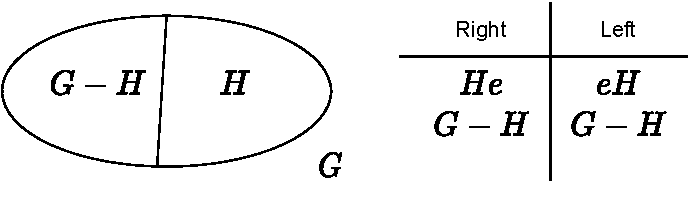
\includegraphics[width=0.65\textwidth]{Figures/as(1).pdf} \\($H=He$ is a right coset, and if there are only two right cosets then the remaining coset must be everything else in $G$, a similar argument can be made for $H's$ left cosets in $G$ )\\
So $H\triangleleft G$ by L 2.6.2. $\blacksquare$
\end{corollary}
Which subgroups have index 2? \ \ $i=2=\frac{o(G)}{o(H)}$ \steezybreak\\
\begin{center}
  $\implies$\ \ \ \ \boxed{o(H)=\frac{1}{2}o(G)}  
\end{center}\steezybreak
Note that according to the set product defn.
\begin{align}
    HK&=\{hk|h\in H, k\in K\} \nonumber 
    \end{align}
It is true for any subgroup $H<G$ that, 
\begin{align}
    HH&=H. \nonumber \\
    \textit{pf:} \ \ \ \ &\subseteq : \text{closure in } H \nonumber \\
    &\supseteq : h=\underset{\in H}{h}\cdot\underset{\in H}{ e} \in  HH \nonumber 
\end{align}
We use this fact in our proof of the lemma below.

\begin{lemma}
Suppose $N<G$. $N\triangleleft G \iff Na\cdot Nb = N{ab} \ \forall a,b \in G$ \steezybreak\\
\textit{Proof:} \steezybreak\\
$\Rightarrow :$  \ \ \ Assume $N\triangleleft G$\steezybreak\\
Take $a,b\in G$
\begin{align}
    NaNb=N(aN)b \underset{L \ 2.6.2}{=}N(Na)b=NNab = Nab .\nonumber
\end{align}
$\Leftarrow :$ \ \ \ Assume $Na\cdot Nb=Nab \ \forall a,b\in G.$\steezybreak\\
Take $a\in G$; we'll show $aN=Na$ (so $N\triangleleft G$ by L 2.6.2)\steezybreak\\
$\subseteq :$ ($aN\subseteq Na$ must be shown)
\begin{align}
    &NaNa^{-1}=Naa^{-1}=N \nonumber\\
    &\text{Right multiply by } a \nonumber\\
    &\implies NaN=Na \nonumber \\
    &aN=eaN\subseteq NaN=Na , \text{ so } aN\subseteq Na \nonumber
\end{align}
$\supseteq :$ ($Na\subseteq aN$ must be shown)\steezybreak\\
\begin{align}
    &Na^{-1}Na=Na^{-1}a=N \nonumber \\
    &\text{Right multiply by } a^{-1} \nonumber\\
    &\implies Na^{-1}N=Na^{-1}; a^{-1}N=ea^{-1}N\subseteq Na^{-1}N=Na^{-1} \nonumber \\
    &\text{So } a^{-1}N\subseteq Na^{-1} \nonumber \\
    &\implies a^{-1}Na\subset N \nonumber \\
    &\implies Na\subset aN \nonumber
\end{align}
$\therefore aN=Na$ and so $N\triangleleft G$ by L 2.6.2. $\blacksquare$
\end{lemma}
\subsubsection{Normal Subgroups Summary}
\begin{align}
    N\triangleleft G &\overset{defn.}{\iff} gng^{-1}\in N \ \ \forall \ n\in N \text{ and } \forall \ g \in G. \nonumber \\
    &\overset{}{\iff} gNg^{-1}\subset N \ \ \forall \ g \in G \nonumber \\
    &\overset{L2.6.1}{\iff} gNg^{-1} = N \ \ \forall \ g \in G \nonumber \\
    &\overset{L2.6.2}{\iff} gN = Ng \ \ \forall \ g \in G \nonumber \\
    &\overset{L2.6.3}{\iff} NaNb = Nab \ \ \forall \ a,b \in G \nonumber 
\end{align}
$N\triangleleft G$ means the set of cosets of $N$ in $G$ has a group structure.\steezybreak\\
$N\triangleleft G$ means:
\begin{enumerate}
    \item $N$ absorbs conjugates:
    \begin{align}
        gng^{-1}\in N \ \ \forall \ g \in G, \ \ \forall \ n \in N. \nonumber 
    \end{align}
    \item The left and right cosets of $N$ are equal
    \begin{align}
        gN=Ng \ \ \forall \ g \in G. \nonumber 
    \end{align}
    \item The cosets combine under binary operations:
    \begin{align}
        NaNb\overset{\star\star\star}{=}Nab \ \ \forall \ a,b \in G. \nonumber
    \end{align}
    \item With this ($\star\star\star$) operation, the cosets form a group (Thm 2.6.1)
\end{enumerate}
\begin{definition}[Quotient Group]
For group $G$ with normal subgroup $N\triangleleft G$, $G/N$ ($G \mod N$)
\begin{align}
    G/N\overset{def}{=}\{\text{(right) cosets of }N \text{ in } G\}\nonumber
\end{align}
\end{definition}
\newpage
\begin{theorem}[Quotient Groups] \hspace{0.01in}\\
if $N\triangleleft G$, then $G/N$ is a group under this operation:
\begin{align}
    Na \underset{\text{in }G/N}{\cdot} Nb = Na \underset{\text{in }G}{\cdot} b \nonumber
\end{align}
\textit{Proof:} We must show that $G/N$ under the defined operation follows the 4 group properties.
\begin{enumerate}[label=\roman*)]
    \item Closure:
    \begin{align}
        NaNb=Nab \nonumber
    \end{align}
    Since $Nab$ is a coset in $G/N$ we are done (closure is built into the defn of the operation)
    \item Associativity:
    \begin{align}
        [NaNb]Nc&=NabNc \nonumber\\
        &= N(ab)c \nonumber \\
        &= Na(bc)  \ \ \ \ (\text{since } G \text{ is assoc.})\nonumber \\
        &= Na(Nbc) \nonumber \\
        &= Na[NbNc] \nonumber
    \end{align}
    \item Identity:
    \begin{align}
        NaNe=Nae=Na\nonumber \\
        NeNa=Nea=Na\nonumber \\
        Ne=N \text{ is the } e \text{ in } G/N \nonumber
    \end{align}
    \item Inverses: $\text{Take }Na\in G/N.$
    \begin{align}
        a\in G &\implies a^{-1} \in G, \text{ so } Na^{-1}\in G/N \nonumber \\
        NaNa^{-1}&=Naa^{-1}=Ne=N \nonumber \\
        Na^{-1}Na&=Na^{-1}a=Ne=N \nonumber 
    \end{align}
    So $(Na)^{-1}=Na^{-1}$. \ \ \ \ \ $\blacksquare$
\end{enumerate}
    
$G/N$ is referred to as the \textit{quotient group} or \textit{factor group} of $G$ by $N$.
\end{theorem}
\begin{lemma}
if $N\triangleleft G$ finite, then
\begin{align}
    o(G/N)=\frac{o(G)}{o(N)}\nonumber
\end{align}
\textit{Proof:}
\begin{align}
    o(G/N)&= \# \text{ of (right) cosets of }N \text{ in }G \nonumber \\
    &= i_G(N)=\frac{o(G)}{o(N)}. \ \ \ \blacksquare \nonumber 
\end{align}
\end{lemma}

\begin{example}
$G=\Z$ under $+$
\begin{align}
    n\Z=\{\text{integer multiples of }n\}< \Z \nonumber
\end{align}
\textit{Claim:} $nZ\triangleleft \Z$, we'll show $n\Z$ absorbs conjugates ($\forall \ h\in H, \ \forall \ g\in G, ghg^{-1}\in H$).\\
Take $z\in \Z$ and $nm\in n\Z$.
\begin{align}
    \underset{g}{z}\ \ \ \ \underset{\cdot \text{ in } G}{+}\ \ \ \ \underset{h}{nm}\ \ \ \ +\ \ \ \ \underset{g^{-1}}{(-z)}=nm \in n\Z \ \ \ \ (\text{Remember that }\Z\text{ is abelian under }+) \nonumber
\end{align}
So $\Z/n\Z$ is a quotient group of $n\Z$ in $\Z$. What are it's elements?
\begin{align}
    G/N&= \{\text{(right) cosets of }N \text{ in }G\}\nonumber \\
    N\cdot 0 &= n\Z+0 = n\Z=[0] \text{ under }\equiv\mod n \nonumber \\
    N\cdot 1 &= n\Z+1 =[1] \text{ under }\equiv\mod n \nonumber \\
    N\cdot 2 &= n\Z+2 =[2] \nonumber\\
    \vdots \nonumber \\
    N\cdot (n-1)&= n\Z+n-1=[n-1] \nonumber \\
    N\cdot n&= n\Z+n=[0] \nonumber 
\end{align}
So $\Z/n\Z= \{[0],[1],[2],...,[n-1]\}$. So $\Z/n\Z$ and $\Z_n$ are the same group (rename the elements to get $\Z_n$).
\end{example}

\begin{example}
Passing from $G\rightarrow G/N$ lets you study properties of $G$ in a smaller group. For instance, oddness or evenness in $\Z$, use $\Z/2\Z$.\steezybreak\\
$\Z/2\Z=\{[0],[1]\}=\{2\Z+0,2\Z+1\}$ or $Z_2=\{0,1\}$ under addition $\equiv\mod 2$

    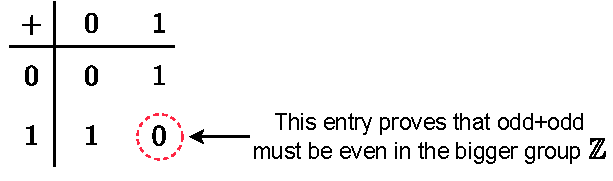
\includegraphics[width=0.65\textwidth]{Figures/Z2-cayley-example-later (1).pdf}

\end{example}

\begin{example}
$M\in GL_2(\R)= \{\text{inv }2\times 2's \text{ with }\R \text{ entries}\}$\steezybreak\\
\textit{Problem:} Show that $M=\begin{pmatrix}
r & 0 \\
0 & 1
\end{pmatrix}M'$ where $r\in \R-\{0\}$ and $det(M')=1$.\steezybreak\\
We'll use $SL_2(\R)=\{\det 1 \text{ matrices}\}\subset GL_2(\R)$.\steezybreak\\
\textit{Claim:} $SL_2(\R)\triangleleft GL_2(\R)$, we've already shown $SL_2(\R)<GL_2(R)$ so we only need to show that $SL_2(\R)$ absorbs conjugates.
\begin{align}
    \text{take }A, \text{ a matrix in } GL_2(\R) \text{ and } B \in SL_2(\R)\nonumber\\
    \det(ABA^{-1})=\det(A)\det(B)\det(A^{-1})=\det(A)(1)(\frac{1}{\det(A)}= (1)(1)=1 \nonumber \\
    \text{So } ABA^{-1}\in SL_2(\R) \nonumber \\
    \therefore SL_2(\R) \triangleleft GL_2(R) \nonumber 
\end{align}
So $GL_2(\R)/SL_2(\R)$ is a group.\steezybreak\\
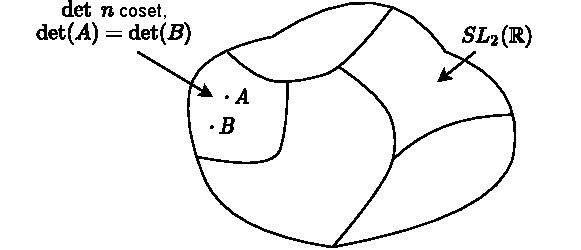
\includegraphics[width=0.5\textwidth]{Figures/aside_sl2(R).pdf}\steezybreak\\
Recall: The cosets are the equivalence classes under "$\equiv \mod H$".
\begin{align}
    A\equiv B \mod SL_2(\R) &\iff AB^{-1}\in SL_2(\R) \nonumber \\
    &\implies \det(AB^{-1})=1 \nonumber \\
    &\implies \det(A)\frac{1}{\det(B)}=1 \nonumber\\
    &\implies \det(A)=\det(B). \ \ \ \ \ \ \ \ \ \text{ (See figure.)}\nonumber 
\end{align}
For any choice of $n\in \R-\{0\}$, the $\det -n$ coset has a natural representative $\begin{pmatrix}
n & 0 \\
0 & 1
\end{pmatrix}$ so we have the $\det-n$ coset
\begin{align}
    \begin{pmatrix}
n & 0 \\
0 & 1
\end{pmatrix}SL_2(\R)\nonumber
\end{align}
Now, take $M\in GL_2(\R)$ and say $\det(M)=r$ ($r\neq 0$ because $M\in GL_2(\R)$), $M$ belongs to exactly one coset:
\begin{align}
    &\det-r \text{ class}:\nonumber\\
    &M\in \begin{pmatrix}
r & 0 \\
0 & 1
\end{pmatrix}SL_2(\R) \implies \exists \ M' \in SL_2(\R) \ni M= \begin{pmatrix}
n & 0 \\
0 & 1
\end{pmatrix}M'\nonumber
\end{align}
(Note $\det(M')=1$ since it is a member of  $SL_2(\R)$.)
\end{example}

\section{Homomorphisms}
\begin{definition}[Homomorphism]
$G,\bar{G}$ groups. A mapping $\phi: G\rightarrow \bar{G}$ is a \textit{homomorphism} if 
\begin{align}
    \phi(a \underset{\cdot \text{ in } G}{\cdot} b)=\phi(a)\underset{\cdot \text{ in } \bar{G}}{\cdot} \phi(b) \ \ \forall \ a,b\in G \nonumber
\end{align}
\end{definition}
Informally, we say $\phi: G \rightarrow \bar{G} $ is a homomorphism if it \textit{splits over products}.
\begin{figure}[h!]
    \centering
    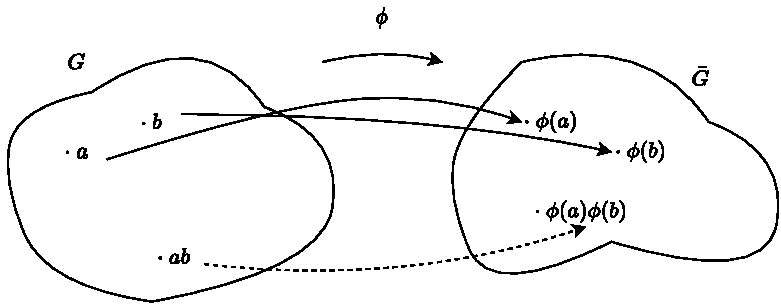
\includegraphics[width=0.85\textwidth]{Figures/homomorphisms_1.pdf}
    \caption{Visualizing A Homomorphism between Groups}
    \label{fig:morphism1fig}
\end{figure}

\begin{figure}[ht!]
    \centering
    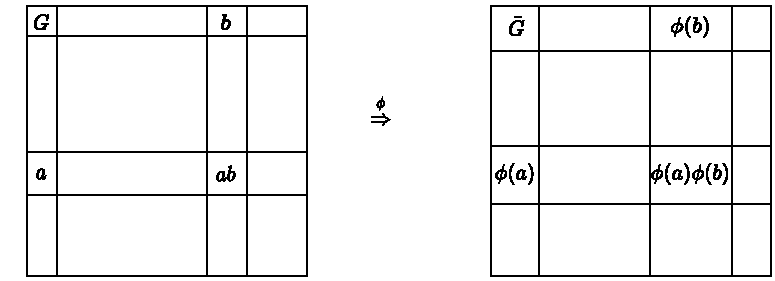
\includegraphics[width=0.85\textwidth]{Figures/homomorphisms_2 (1).pdf}
    \caption{Visualizing A Homomorphism between Groups}
    \label{fig:morphism2fig}
\end{figure}

\begin{figure}[h!]
    \centering
    
\includegraphics[width=0.55\textwidth]{Figures/homomorphisms_3 (1).pdf}
    \label{fig:morphism3fig}
\end{figure}
\newpage
\subsubsection{Some Examples of Homomorphisms}
\begin{example}
Trivial homomorphism:
\begin{align}
    &\phi: G\rightarrow \bar{G} \nonumber \\
    &\phi(x)=\ \underset{\in \bar{G}}{e} \ , \ \forall \ x\in G. \nonumber
\end{align}
Take $x,y\in G$
\begin{align}
    \phi(x)&=e \ \ (\text{by defn.}) \nonumber\\
    \phi(y)&=e \ \nonumber \\
    \phi(\ \underset{\in G}{xy}\ )&=e=e\cdot e =\phi(x)\cdot \phi(y). \nonumber\\
    &\therefore \phi \text{ is a homomorphism since it \textit{splits} over products.} \nonumber 
\end{align}
For the readers interested in category theory: In the category of groups (or of modules), a \textit{zero morphism} is a homomorphism $f : G \rightarrow \bar{G}$ that maps all of $G$ to the identity element of $\bar{G}$ (exactly the trivial homomorphism!). The zero object in the category of groups is the trivial group $1 = \{1\}$, which is unique up to isomorphism.
\end{example}
\begin{example}
Identity Homomorphism.
\begin{align}
    &\phi: G\rightarrow G \nonumber \\
    &\phi(x)=x, \ \forall \ x\in G \nonumber 
\end{align}
We can easily see this mapping splits over products, let $x,y\in G$:
\begin{align}
    \phi(x)&=x \nonumber \\
    \phi(y)&=y \nonumber \\
    \phi(xy)&=xy=\phi(x)\cdot \phi(y) \nonumber 
\end{align}
\end{example}

\begin{example}
Inclusion homomorphism: $H<G$, 
\begin{align}
    &\phi : H\rightarrow G \nonumber \\
    &\phi(h)= h \nonumber \ \forall h \in H \\
    \phi(h)&=h\in G, \ \ \phi(z)=z\in G \nonumber \\
    \phi(hz)&=hz\in G = \phi(h)\cdot \phi(z) \nonumber
\end{align}
"Inclusion" is a shift in perspective.
\end{example}

\begin{example}
Conjugation by $g\in G$.
\begin{align}
    \text{fix } &g \in G. \nonumber \\
    &\phi_g: G\rightarrow G \nonumber \\
    &\phi_g(x)=gxg^{-1} \ \forall \ x \in G \nonumber \\
    \phi_g(xy)=gxyg^{-1}&=gxeyg^{-1}=gx(g^{-1}g)yg^{-1} \nonumber \\
    &=(gxg^{-1})(gyg^{-1}) \nonumber \\
    &=\phi_g(x)\cdot \phi_g(y). \nonumber \\
    \therefore \phi_g \text{ is a homomorphism on }G. \nonumber 
\end{align}
\end{example}

\begin{example}
Determinant
\begin{align}
    G&=GL_2(\R) \ \text{ under matrix multiplication} \nonumber \\
    \bar{G}&=\R-\{0\} \ \text{ under multiplication } \nonumber \\
    &\phi:G\rightarrow \bar{G} \nonumber\\
    \text{ defined by } &\phi(M)=\det(M) \nonumber\\
    \phi(MN)=\det(MN)&=\det(M)\det(N)=\phi(M)\phi(N) \nonumber 
\end{align}
\end{example}

\begin{example}
Evaluation map.
\begin{align}
    &G= \{\text{real-valued mappings: } \R \rightarrow \R \} \text{ under }+ \nonumber \\
    \text{Let }&f,g,h:\R \rightarrow \R \nonumber \\
    &(f+g)+h=f+(g+h) \ \ \ \ \ e\text{ is }f(x)=0 \ \ \ \ \ [f(x)]^{-1}=-f(x) \nonumber \\
    &\text{Now let } \bar{G} = \R \text{ under }+ \nonumber \\
    &\text{fix }r\in \R \nonumber \\
    &\text{Define } \phi_r:G\rightarrow \bar{G} \text{ by } \phi_r(f(x))=f(r) \nonumber \\
    &\text{ Take } f(x),g(x)\in G \nonumber \\
    &\phi_r[f(x)\cdot g(x)]=(f+g)(r)=\underset{\in \R}{f(r)+g(r)} = \phi_r(f(x))+\phi_r(g(x)) \nonumber
\end{align}
\end{example}

\textit{More examples of Homomorphisms can be found in Herstein's Topics in Algebra 2 ed.  pgs. 55-56}\steezybreak\\

\begin{lemma}
$N\triangleleft G$,
\begin{align}
    \text{Define } &\phi: G\rightarrow G/N  \ \ \ \ (\text{Remember: }G/N \text{ is the set of cosets of } N \text{ in }G ) \nonumber \\
    \text{by } &\phi(g)=Ng \ \ \forall g \in G \nonumber
\end{align}
Then $\phi$ is a surjective homomorphism, called the "canonical" or "natural" map. \\
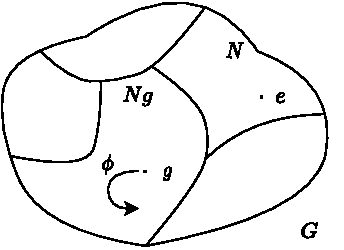
\includegraphics[width=0.45\textwidth]{Figures/natural_map.pdf}This map takes $g\in G$ to the coset in which it sits. \\

\noindent\textit{Proof:}
\begin{align}
    &\text{Let }g,g'\in G \nonumber \\
    &\phi(g\cdot g')= N(g\cdot g')\underset{\cdot \text{ in }G/N}{=} NgNg' = \phi(g)\cdot \phi(g'). \nonumber \\
    &\therefore \ \phi \text{ is a homomorphism.} \nonumber
\end{align}
$\phi$ is surjective: \\
\begin{align}
    \text{Let }Nx \in G/N \ \ \ (\text{i.e. } Nx \text{ is a random coset}) \nonumber \\
    \phi(x)=Nx \nonumber
\end{align}
so $x$ serves as a pre-image for $Nx$. $\blacksquare$
\end{lemma}


\begin{lemma}
Given $\phi: G\rightarrow \bar{G}$ a homomorphism,
\begin{enumerate}[label=\roman*)]
    \item $\phi(e)=\bar{e}$
    \item $\phi(g^{-1})=[\phi(g)]^{-1}$
\end{enumerate}
\textit{Proof:}
\begin{enumerate}[label=\roman*)]
    \item \begin{align}
        &\phi(e)\cdot \bar{e}=\phi(e)=\phi(e\cdot e)=\phi(e)\cdot\phi(e) \nonumber \\
        \implies & \not {\phi(e)}\cdot \bar{e}=\not{\phi(e)}\cdot\phi(e) \ \ \ \ \text{by left cancellation of $\phi(e)$ in }\bar{G} \nonumber \\
        \implies &\bar{e}=\phi(e) \nonumber
    \end{align} 
    \item Inverses. Take $g\in G$, $\phi(g)$ has a unique inverse in $\bar{G}$. We will show $\phi(g^{-1})$ satisfies inverse property
    \begin{align}
        &\phi(g^{-1})\cdot \phi(g)= \phi(g^{-1}\cdot g)=\phi(e)=\bar{e} \nonumber \\
        &\phi(g)\cdot\phi(g^{-1})=\phi(g\cdot g^{-1})=\phi(e)=\bar{e} \nonumber
    \end{align}
    So $\phi(g^{-1})=[\phi(g)]^{-1}$\\
    Since $\phi(g^{-1})$ does the job of an inverse and inverses must be unique, $\phi(g^{-1})$ is the unique inverse of $\phi(g)$. $\blacksquare$ 
\end{enumerate}
\end{lemma}
\newpage
\begin{definition}[Kernel]
Let $\phi:G\rightarrow \bar{G}$ be a homomorphism. The \textit{kernel} of $\phi$ is the set of elements in $G$ that $\phi$ sends to the identity element in $\bar{G}$
\begin{align}
    K= \{g\in G | \phi(g)=\bar{e}\}. \nonumber
\end{align}
Note, $K\neq \{\}$ because $e\in K$ by L 2.7.2 (i). $K$ is also commonly denoted ``$\text{ker}\ \phi$" or ``$\text{ker}(\phi)$" to avoid ambiguity when there are multiple homomorphisms being discussed.\\
\begin{center}
    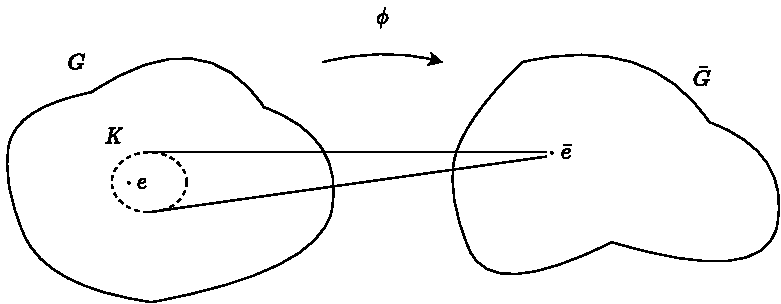
\includegraphics[width=0.65\textwidth]{Figures/kernel_hom.pdf}
\end{center}
\end{definition}

\begin{lemma}
$\phi:G\rightarrow \bar{G}$ hom. with kernel $K$. Then $K\triangleleft G$. \steezybreak\\

\noindent \textit{Proof:} We know $e\in K$ so $K$ is non-empty and L 2.4.1 applies (we begin by showing $K<G$ then to show 'normal' part we will show $K$ absorbs conjugates).
\begin{enumerate}[label=\roman*)]
    \item Closure. Let $a,b\in K$
    \begin{align}
        &\phi(ab)\underset{\phi \text{ hom.}}{=}\phi(a)\phi(b)\underset{a,b\in K}{=} \bar{e}\bar{e}=\bar{e} \nonumber \\
        &\therefore ab\in K. \nonumber 
    \end{align}
    \item Inverses. Let $a\in K$  (remember $a\in G \implies a^{-1}\in G$)
    \begin{align}
        &\phi(a^{-1})=[\phi(a)]^{-1}=[\bar{e}]^{-1}=\bar{e}\nonumber \\
        &\therefore a^{-1}\in K. \nonumber 
    \end{align}
\end{enumerate}
By Lemma 2.4.1 $K<G$. \\
Now to show that $K$ is normal we will show it absorbs conjugates. Take $x\in K$ and $g\in G$.
\begin{align}
    \phi(gxg^{-1})&= \phi(g)\phi(x)\phi(g^{-1}) = \phi(g)\bar{e}\phi(g^{-1})\nonumber \\
    &= \phi(g)\phi(g^{-1})=\phi(g\cdot g^{-1})= \phi(e)=\bar{e}. \nonumber
\end{align}
Since $gxg^{-1}\in K$, $K\triangleleft G$. $\ \ \blacksquare$
%\textit{This proof is incomplete, will finish later today}
\end{lemma}

\begin{proposition}
$\phi:G\rightarrow \bar{G}$ hom. with kernel $K$.
\begin{align}
    \phi \text{ is injective } \iff K= \{e\}\nonumber
\end{align}
\textit{Proof:}\\
$\Rightarrow \ :$ Assume $\phi$ injective.\\
\begin{align}
    \text{Take }k\in K \nonumber \\
    \phi(k)=\bar{e}=\phi(e) \nonumber \\
    \text{If }k\neq e , \phi \text{ inj. } \implies \phi(k)\neq \phi(e)\ ...\ \Rightarrow \Leftarrow \nonumber \\
    \therefore k \text{ must be }e; \ K=\{e\} \nonumber
\end{align}
$\Leftarrow \ :$ Assume $K=\{e\}$.\\
Injective means distinct elements stay distinct. We will use contraposition to show $\phi$ is injective. \steezybreak\\ %(i.e. rather than show $A\implies B$ is true we will show the equivalent contraposition $\lnot B \implies \lnot A$ is true). \\
(i.e. we want to show $a\neq b \implies \phi(a)\neq \phi(b)$ so we will equivalently show $\phi(a)=\phi(b) \implies a= b$ which is the contraposition of the desired implication.)\steezybreak\\
By contrapositive: if 2 images are not distinct, then their pre-images are not distinct. Consider:
\begin{align}
    \phi(g_1)=\phi(g_2)\nonumber
\end{align}
Now left multiplying by $[\phi(g_1)]^{-1}$
\begin{align}
    \bar{e}&=[\phi(g_1)]^{-1}\phi(g_2)\nonumber \\
    &= \phi(g_1^{-1}g_2) \nonumber \\
    &\therefore g_1^{-1}g_2\in K \nonumber
\end{align}
now since $K=\{e\}\ \ \implies g_1^{-1}g_2=e \implies g_1=g_2$\\
$\therefore \ \phi$ is injective. $\ \ \blacksquare$
%\textit{This proof is incomplete, will finish later today}
\end{proposition}

Let's have a look at calculating Kernels of homomorphisms.
\begin{example}
Fix $g\in G$ and define $\phi_g: G\rightarrow G$ by $\phi_g(x)=gxg^{-1}\ \forall \  x \in G$. \\
Now, take $k\in K$.
\begin{align}
    \phi_g(k)=e=gkg^{-1} \nonumber
\end{align}
solve for $k$
\begin{align}
    g&=gk\nonumber \\
    g^{-1}g&=k\nonumber \\
    e&=k\nonumber 
\end{align}
$\therefore K = \{e\}$, so $\phi_g$ is injective by the proposition above.
\end{example}

\begin{example}
$\phi:\overset{\text{mat. mult.}}{GL_n(\R)}\rightarrow \overset{\text{mult.}}{\R-\{0\}}$ \\
$\phi(M)=\det(M)$. \\
Suppose $M\in \ker(\phi)$, then
\begin{align}
    \phi(M)=\det(M)=1 \nonumber
\end{align}
So $M\in \ker(\phi) \iff \det(M)=1$ which means
\begin{align}
    \ker(\phi)&=\{n\times n \text{ matrices with entries in }\R \text{ having determinant }1\}\nonumber \\
    &=SL_n(\R) \neq \{I_n\} \nonumber
\end{align}
$\therefore \phi$ is \textit{not} injective.
\end{example}

\begin{example}
Fix $r\in \R$. \\
Consider $\phi_r: \{\text{real valued functions }\}\rightarrow \R$ defined by
\begin{align}
    \phi_r(f)=f(r)\nonumber
\end{align}
If $f\in \ker(\phi_r)$ then $\phi_r(f)=0$ since $0$ is the "$e$" in $\R$ under $+$. \\
So $\ker(\phi_r) = \{\text{set of functions with root at } r\} \neq \{f(x)=0\}$ so $\phi_r$ is \textit{not} injective.
\end{example}

\begin{example}
Assume $N\triangleleft G$ and consider again the $\phi$ from Lemma 2.7.1 going from $G$ to the group of cosets of $N$ in $G$, $G/N$:
\begin{align}
    \phi: G\rightarrow G/N \nonumber \\
    \phi(g)= Ng \nonumber
\end{align}
What is $\ker(\phi)$ in this case? If $g\in \ker(\phi)$ then
\begin{align}
    \phi(g)=e= N \ \ \ \text{(Remember, $N$ is the $e$ in $G/N$)}\nonumber \\
    Ng=\phi(g)=N \nonumber
\end{align}
$g$'s coset is $N$. So every element of $N$ is in $\ker(\phi)$.\\
$\therefore \ \ker(\phi)=N$. 
\end{example}

\begin{definition}[Image of Group under a Homomorphism]
$\phi: G\rightarrow \bar{G}$ group hom., then 
\begin{align}
    \phi(G)= \{\phi(g)\ | \ \forall g\in G\}\nonumber
\end{align}
is the \textit{image of }$G$ \textit{under} $\phi$.\steezybreak\\
Note that $\phi(G)=\bar{G}\iff \phi \text{ is surjective (onto)}$. Prove this as an exercise.
\end{definition}
\begin{proposition}
$\phi:G\rightarrow \bar{G}$ group hom.\steezybreak\\
Then $\phi(G)< \bar{G}$\steezybreak\\
\textit{Proof:} $\phi(G)$ is non-empty since $\phi(e)=\bar{e}\in \phi(G)$ so L 2.4.1 applies
\begin{enumerate}[label=\roman*)]
    \item Closure: take $y,y'\in \phi(G)$, then
    \begin{align}
        \text{there exists } &x,x'\in G \ni \phi(x)=y \text{ and } \phi(x')=y' \nonumber \\
        &xx'\in G \text{   , since } G \text{ is a group.} \nonumber \\
        &\phi(xx')=\phi(x)\phi(x')=yy' \nonumber \\
        \therefore \ &yy'\in \phi(G) \nonumber
    \end{align}
    \item Inverses: Take $y\in \phi(G), \ \implies \exists \ x\in G \ni \phi(x)=y$\\
    \begin{align}
        &y^{-1}=[\phi(x)]^{-1}=\phi(x^{-1})\nonumber\\
        &x^{-1}\in G \text{   , since } G \text{ is a group,} \nonumber \\
        \therefore \ &y^{-1}\in \phi(G). \ \ \ \ \ \ \blacksquare \nonumber
    \end{align}
\end{enumerate}
\end{proposition}

\begin{tcolorbox}
    $\star$ \textbf{Important Note:} A homomorphism $\phi: G\rightarrow \bar{G}$ that is not surjective can be redefined so that it is surjective like this:\\
    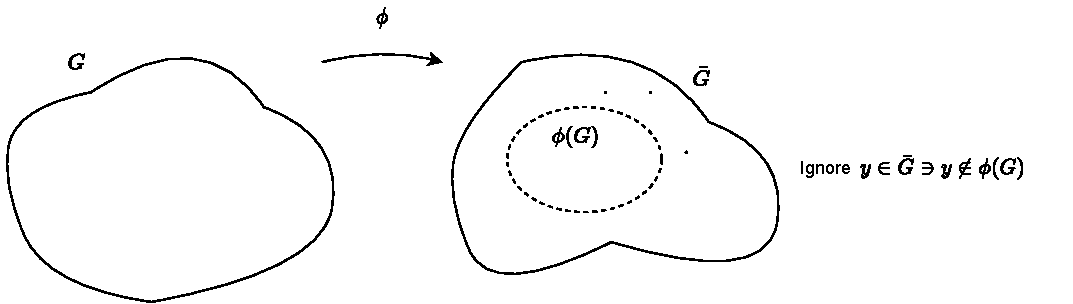
\includegraphics[width=\textwidth]{Figures/make_surj1.pdf}\\
    i.e. discard non participants in the map. We can toss these out with no effect on the map.\\
    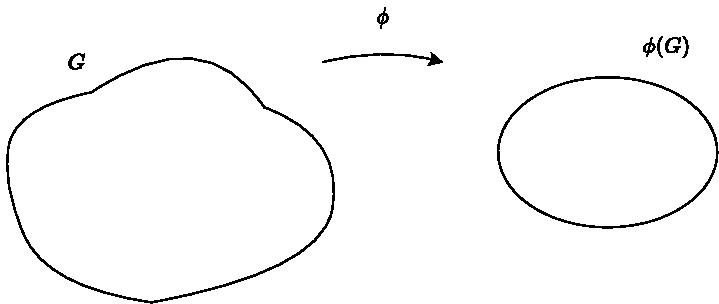
\includegraphics[width=0.7\textwidth]{Figures/make_surj3.pdf}\\
    Instead of $\phi:G\rightarrow \bar{G}$; redefine as $\phi: G\rightarrow \phi(G)$ so now $\phi$ is surjective.
\end{tcolorbox}

\begin{definition}[Isomorphism]
An \textit{isomorphism} between groups is a bijective homomorphism. \steezybreak\\
$G$ and $G^*$ are isomorphic groups, denoted $G\approx G^*$ (or often $G\simeq G^*$, though we prefer the former convention) if $\exists$ an isomorphism from $G$ to $G^*$.
\begin{align}
    G\approx G^* \iff \exists \ \sigma: G\rightarrow G^* \ni 
    \begin{cases}
      \sigma \text{ is a homomorphism}\\
      \sigma \text{ is injective}\\
      \sigma \text{ is surjective}
    \end{cases} \nonumber 
\end{align}
\end{definition}
some day I will type up handout 3 but for now look at it while you read along, the $\tilde{G}$ is a subgroup of $G_{17}$. Let's have a look at $\Z_8$
\begin{align}
    \Z_8=\langle 1 \rangle =\langle 3 \rangle = \{3^n\ | \ n\in \Z \} \ (\text{Remember, }\Z_8\text{'s group operation is } + \text{ mod }8).\nonumber\\
    \tilde{G}=\langle 2 \rangle = \{2,4,8,16,15,...,1\}=\langle 8 \rangle = \{8^n\ | \ n\in \Z\} \ (\text{Remember, }G_{17}\text{'s group operation is } \times \text{ mod }17).\nonumber
\end{align}
\newpage
\begin{multicols}{2} % two columns
        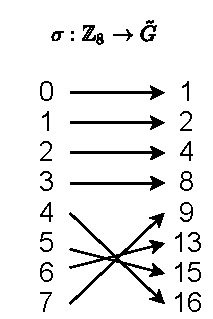
\includegraphics[width=0.35\textwidth]{Figures/iso_example_Z8_G17.pdf} 
        
        To show that $\Z_8 \approx G_{17}$ we will construct a mapping $\sigma$ from $\Z_8$ to $G_{17}$ that is a homomorphism and is a bijection. To show the first property we show that $\sigma$ splits over products for generators of each of the groups which is sufficient to show it splits for all products. 
        \begin{enumerate}
            \item $\sigma(3^n)=8^n$\\
            $\sigma(3^m 3^n)= \sigma(3^{m+n})=8^{m+n}=8^m8^n=\sigma(3^m)\sigma(3^n), \ \ \therefore \sigma $ hom.
            \item From the figure the homomorphism we have defined is obviously a 1-1 correspondence so $\sigma$ is a bijection. %(if this isn't obvious to you, convince yourself with the diagram that every unique element in $\tilde{G}$ has preimage in $\Z_8$ (surjective) and that each of those images are unique meaning if $z\neq y$ then $\phi(z)\neq \phi(y)$ (injective)).
        \end{enumerate}
        $1 \ \& \ 2$ together $\implies $ $\sigma$ is an isomorphism.
\end{multicols}

\noindent$\boxed{\textbf{Important Fact:}}$ Any two cyclic groups of the same order are isomorphic.\\
This is true via the map $\phi: \langle a\rangle \rightarrow \langle b \rangle $ (Where $a$ is the generator of one group and $b$ the generator of another) defined by $\phi(a^n)=b^n$, note that the Law of Exponents for groups implies that $\phi$ is a homomorphism. It can be easily checked that $\phi$ is a bijection. \steezybreak\\

\begin{corollary}
If $G$ is cyclic of order $n$, then $G$ is isomorphic to $\Z_n$.\\
\begin{align}
    G\approx \Z_n . \ \ \leftarrow (\text{ Note that }\Z_n \text{ is cyclic generated by } 1.)\nonumber
\end{align}
\end{corollary}

\begin{proposition}
$\approx$ is an equivalence relation on the set of all groups (finite).\\
\textit{Proof:} We need to show that $\approx$ is reflexive, symmetric, and transitive.
\begin{enumerate}
    \item Reflexive: $G\approx G$ via the identity map
    \item Symmetric: Assume $G\approx G^*$. This means $\exists$ bijective homomorphism $\sigma: G\rightarrow G^*$. By Lemma 1.2.3 $\sigma$ is bijective $\iff$ $\sigma$ has an inverse mapping $\sigma^{-1}$. So $\exists$ $\sigma^{-1}: G^*\rightarrow G$ which satisfies
    \begin{align}
        \sigma^{-1}\circ \sigma &= I_G \nonumber \\
        \sigma\circ \sigma^{-1}&=I_{G^*}\nonumber
    \end{align}
    Note that $(\sigma^{-1})^{-1}=\sigma $, so $\sigma^{-1}$ has an inverse mapping (namely $\sigma$) so $\sigma^{-1}$ is a bijection.\\
    \textit{Claim:} $\sigma^{-1}$ is a homomorphism: take $x^*,y^*\in G^*$
    \begin{align}
        \sigma \text{ surj. } \implies \ \exists x\in G \ni \sigma(x)=x^* \ \text{ and} \nonumber \\
        \sigma^{-1}(x^*)=\sigma^{-1}(\sigma(x))=I_G(x)=x \nonumber
    \end{align}
    Similarly,
    \begin{align}
        \sigma \text{ surj. }&\implies \ \exists y\in G \ni \sigma(y)=y^* \nonumber \\
        \sigma^{-1}(x^*y^*)&=\sigma^{-1}(\sigma(x)\sigma(y))\underset{\sigma \text{ hom.}}{=}\sigma^{-1}(\sigma(xy))=xy=\sigma^{-1}(x)\sigma^{-1}(y) \nonumber \\
        &\therefore \sigma^{-1} \text{ is a bijective hom.} \nonumber \\
        &\therefore G^*\approx G, \approx \text{ is symmetric}. \nonumber
    \end{align}
    \item Transitive: Assume $G\approx G^*$ and $G^*\approx \bar{G}$
    \begin{align}
        G\approx G^* &\implies \ \exists \ \sigma: G\rightarrow G^* \ \text{ Bijective hom.} \nonumber \\
        G^*\approx \bar{G} &\implies \ \exists \ \tau: G^* \rightarrow \bar{G} \ \text{ also Bijective hom.}\nonumber
    \end{align}
    Then $\tau \circ \sigma: G\rightarrow \bar{G} $ is a bijection by L.1.2.2 (composition of mappings). We claim that, moreover, $\tau \circ \sigma$ is a homomorphism:\\
    Take $x,y\in G$
    \begin{align}
        (\tau \circ \sigma) (xy)&=\tau(\sigma(xy))\underset{\sigma \text{ hom.}}{=}\tau(\sigma(x)\underset{\cdot \text{ in } G^*}{\cdot}\sigma(y)) = \tau(\sigma(x))\underset{\cdot \text{ in } \bar{G}}{\cdot} \tau(\sigma(y))\nonumber \\
        &=(\tau \circ \sigma)(x)\cdot (\tau\circ \sigma)(y) \nonumber \\
        &\therefore \tau\circ \sigma \text{ is a homomorphism.} \nonumber\\
        &\therefore \tau\circ \sigma \text{ is a bijective hom. }\implies \text{ Isomorphism} \nonumber \\
        &\therefore G\approx \bar{G}, \text{ so } \approx \text{ is transitive.} \ \ \blacksquare \nonumber
    \end{align}
\end{enumerate}
\end{proposition}

\begin{figure}
    \centering
    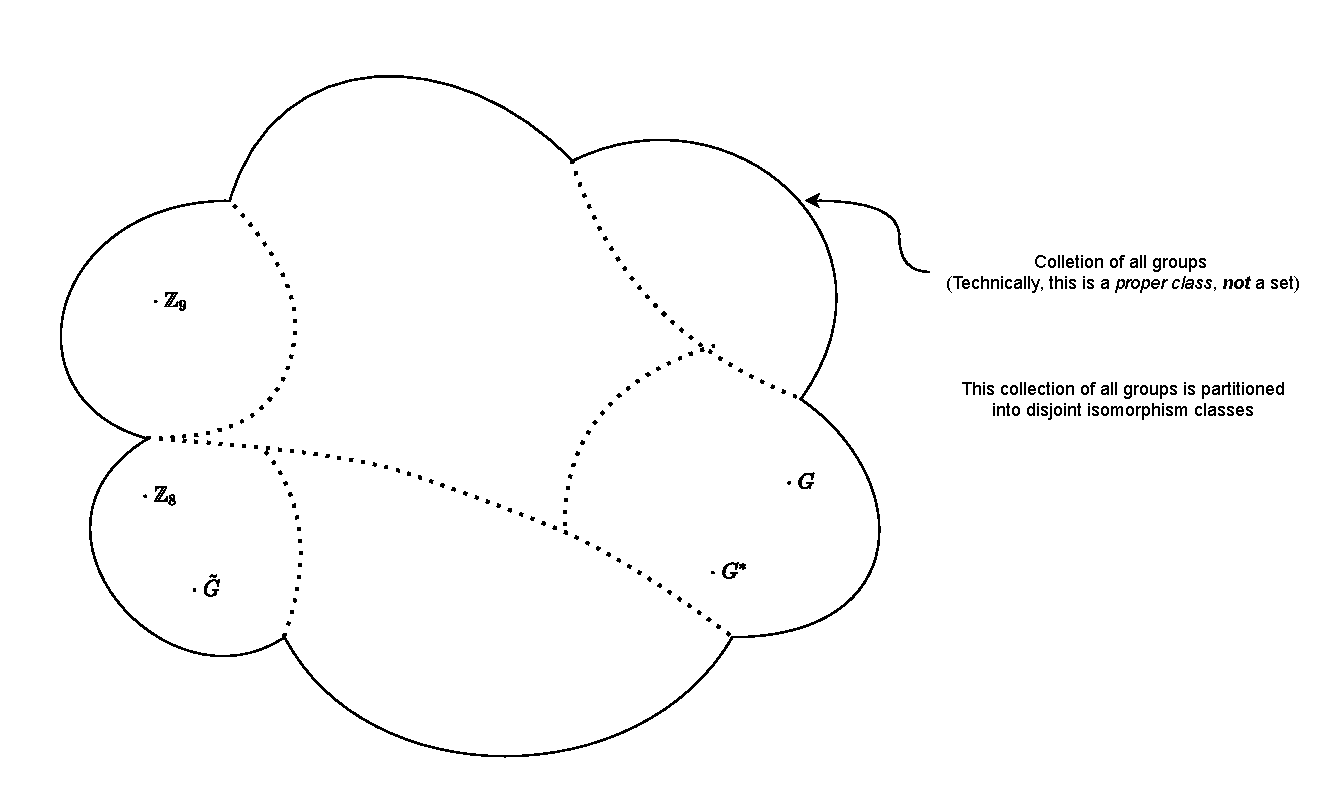
\includegraphics[width=\textwidth]{Figures/ClassofGroups_part (1).pdf}
    \caption{Collection of All Groups is a Proper Class, Isomorphism partitions this class into disjoint isomorphism classes}
    
    \label{fig:my_label}
\end{figure}
\subsection*{Some Ways that Groups fail to be Isomorphic}
\begin{enumerate}
    \item Different Orders
    \item One is cyclic, other is not.
    \item One is abelian, other is not.
    \item Different subgroup lattices
    \item Different order tables
    \item Different \# of Squares
\end{enumerate}
\begin{tcolorbox}
    \begin{center}
        $\star\star\star$ \textbf{Read up to this point to Complete Homework 5 (Located in \ref{sec:HW5})} $\star\star\star$
    \end{center}
    \end{tcolorbox}
\newpage
\setcounter{dummy}{0}
\begin{theorem}[The First Isomorphism Theorem] 
If $\phi$ is a surjective group homomorphism from $G$ to $\bar{G}$ with kernel $K$, then
\begin{align}
    G/K\approx \bar{G} \nonumber
\end{align}
\textit{Proof:}\\
$K\triangleleft G \implies G/K$ is a quotient group (consisting of cosets of $K$ in $G$, $KxKy=Kxy$). We learn about $\bar{G}$ by studying $G/K$. Recall the canonical map from Lemma 2.7.1,
\begin{align}
    \sigma : G \rightarrow G/K \nonumber \\
    \sigma(g)=Kg \nonumber
\end{align}
Now, to show $G/K$ and $\bar{G}$ are isomorphic we must demonstrate that there exists a bijective homomorphism between them. We want a $\tau$ like the one in the diagram below.\steezybreak\\

\noindent Here's the situation: \\
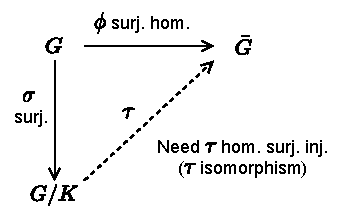
\includegraphics[width=0.5\textwidth]{Figures/1stiso_diag1.pdf} \\
Define $\tau: G/K \rightarrow \bar{G}$ as follows, $\tau(Kg)=\phi(g)$, is $\tau$ well-defined? (i.e. is $\tau$ a mapping?)\steezybreak\\
Potential problem: $Kg$ can have more than one preimage under $\sigma$.\\
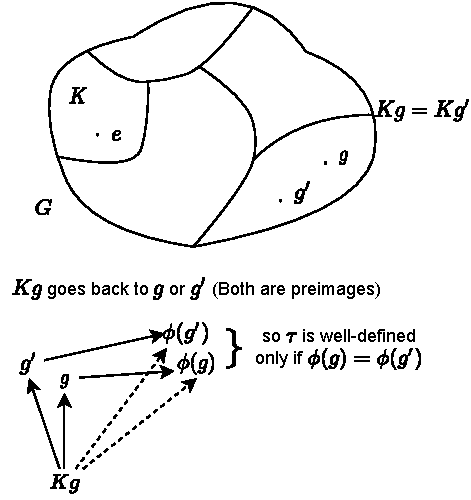
\includegraphics[width=0.5\textwidth]{Figures/1stIso_diag2.pdf}\\
\begin{align}
    \text{Assume }&Kg=Kg' \nonumber \\
    &g'\in Kg'=Kg \nonumber \\
    &\therefore \exists \ k\in K \ni g'=kg \nonumber \\
    \phi(g')&=\phi(kg)=\phi(k)\phi(g)=\bar{e}\phi(g)=\phi(g). \nonumber
\end{align}
Kernel is necessary coset. \\
$\therefore$\\
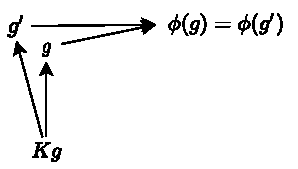
\includegraphics[width=0.45\textwidth]{Figures/1stIso_diag3.pdf} \\
$\therefore \ \tau$ is well-defined. \\
Now it remains to show that $\tau$ is a homomorphism and is bijective. 
 
\textbf{$\tau$ homomorphism:}\\
\begin{align}
    &\tau : G/K \rightarrow \bar{G}, \text{ take } Kg,Kh\in G/K \nonumber \\
    &\tau(KgKh)=\tau(Kgh)=\phi(gh)=\phi(g)\phi(h)= \tau(Kg)\tau(Kh). \nonumber
\end{align} 
So $\tau$ is a homomorphism.\\
To show that $\tau$ is a bijection we will use Lemma 1.2.3 and show that $\tau$ has an inverse mapping. \\
\begin{align}
    &\text{Define }\mu : \bar{G}\rightarrow G/K \text{ by }\nonumber \\
    &\mu(\bar{g})=Kg \ \text{Where }g\text{ is a preimage for }\bar{g} \text{ under }\phi, \text{  (think of $\bar{g}$ as $\phi(g)$)} \nonumber
\end{align}
Is $\mu$ well-defined? We know at least one preimage exists because $\phi$ is surjective by assumption... what if $\bar{g}$ has more than one preimage?
\begin{align}
    \text{Assume } \bar{g}=\phi(g)=\phi(h) \nonumber
\end{align}
Is $Kg=Kh$?
\begin{align}
    \phi(g)&=\phi(h) \nonumber \\
    \implies \phi(g)[\phi(h)]^{-1}&=\bar{e} \nonumber \\
    \implies \phi(g)\phi(h^{-1})&=\bar{e} \nonumber \\
    \implies \phi(gh^{-1})&=\bar{e} \nonumber \\
    \therefore gh^{-1}\in K = \ker\phi \nonumber
\end{align}
Now $gh^{-1} \in K$ implies both $g\in Kg$ (since $e\in K$) and $g\in Kh$ (since $gh^{-1} \in K$ and $gh^{-1}h\in Kh$), therefore $Kg=Kh$ (They must be identical since they are not disjoint, since cosets are equivalence classes)\\
$\therefore \ \mu$ is well-defined 
\begin{align}
    (\tau \circ \mu)(\bar{g})=\tau(\mu(\bar{g}))=\tau(Kg)=\phi(g)=\bar{g} \nonumber \\
    \therefore \ (\tau\circ\mu)= I_{\bar{G}} \nonumber \\
    (\mu \circ \tau)(Kg)=\mu(\tau(Kg))=\mu(\phi(g))=Kg \nonumber \\
    \therefore (\mu\circ\tau)=I_{G/K} \nonumber
\end{align}
So $\tau$ has an inverse $\mu$ making $\tau$ a bijective homomorphism (Isomorphism).
\begin{align}
    \therefore G/K \approx \bar{G} \ \text{ via } \tau \ \ \ \ \ \ \blacksquare \nonumber
\end{align}
%This proof is incomplete, will finish soon, though you should be able to see where this is headed :) we will use the canonical map from L 2.7.1 and use this map to define another map which is a bijective homomorphisms from $G/K$ to $\bar{G}$ ( we first have to construct it an show its well-defined (is a mapping))
\end{theorem}

\subsection*{$H<G$, Some Easy ways to tell if $H\triangleleft G$}
Recall
\begin{align}
    H\triangleleft G &\iff ghg^{-1}\in H \ \forall \ g\in G, \forall \ h\in H \nonumber \\
                     &\iff gH=Hg \ \forall \ g\in G \nonumber \\
                     &\underset{L 2.6.2}{\iff} gHg^{-1}=H \ \forall \ g\in G. \nonumber
\end{align}
\begin{enumerate}
    \item (Trivials) $G\triangleleft G$ because $g\hat{g}g^{-1}\in G$ by closure of $G$. $\{e\}\triangleleft G$ because $geg^{-1} \in \{e\} \ \forall \ g\in G$.
    \item Useful fact (after Lemma 2.6.2): $H<G$, $i_G(H)=2$, then $H\triangleleft G$ and $\frac{o(G)}{o(H)}=2\implies o(H)=\frac{1}{2}o(G)$
    \item \begin{enumerate}[label=\roman*)]
        \item $Z(G)\triangleleft G$ (Homework \#5)
        \item $H<Z(G) \implies H\triangleleft G$
        \begin{align}
            ghg^{-1}=gg^{-1}h=h\in H \nonumber
        \end{align}
        \item $G$ abelian $\implies $ every subgroup of $G$ is normal in $G$.\\
        \begin{align}
            Z(G)=G \ \ \text{(use (ii))}\nonumber
        \end{align}
    \end{enumerate}
    \item If $H$ is the only subgroup of its order $\subset G$, then $H\triangleleft G$.\\
    \textit{Proof:} Fix $g\in G$\\
    \textbf{Claim 1:} $gHg^{-1}< G$, first we note that $e\in H$ so $geg^{-1}\in gHg^{-1}$, therefore $gHg^{-1}$ is non-empty and so Lemma 2.4.1 applies.
    \begin{enumerate}
        \item Closure: $ghg^{-1},gh'g^{-1} \in gHg^{-1}$, \\
        \begin{align}
            (ghg^{-1})(gh'g^{-1})=g \underset{\in H}{(hh')}g^{-1} \in gHg^{-1}.\nonumber
        \end{align}
        \item Inverses: 
        \begin{align}
            (ghg^{-1})^{-1}=(g^{-1})^{-1}h^{-1}g^{-1}=g\underset{\in H}{h^{-1}}g^{-1} \in gHg^{-1} \ \ \ \ \blacksquare \ \ \ \ \text{(Claim 1 Proven)}\nonumber
        \end{align}
    \end{enumerate}
    \textbf{Claim 2:} $o(gHg^{-1})=o(H)$\steezybreak\\
    \begin{align}
        \text{Define } &\sigma:H\rightarrow gHg^{-1} \nonumber \\
        &\sigma(h)=ghg^{-1} \nonumber 
    \end{align}
    To show $\sigma$ is a bijection we'll show $\sigma^{-1}$ exists (L 1.2.3). 
    \begin{align}
        \text{Define } \mu:gHg^{-1} \rightarrow H \nonumber \\
        \mu(ghg^{-1})=g^{-1}(ghg^{-1})g =h \nonumber
    \end{align}
    operations make $\mu$ well-defined. Now we will show $\mu=\sigma^{-1}$.
    \begin{align}
        (\mu \circ \sigma)(h)=\mu(\sigma(h))=\mu(ghg^{-1})=h\nonumber \\
        \text{so }(\mu\circ \sigma)=I_H\nonumber \nonumber \\
        (\sigma\circ \mu)(ghg^{-1})=\sigma(\mu(ghg^{-1}))=\sigma(h)=ghg^{-1} \nonumber\\
        \text{so }(\sigma \circ \mu )=I_{gHg^{-1}}\nonumber
    \end{align}
    $\therefore \ \mu=\sigma^{-1}$ so $\sigma$ is a bijection.\\
    So there is a one-to-one correspondence between $gHg^{-1}$ and $H$ so $o(gHg^{-1})=o(H)$. But $H$ is the only subgroup of $o(H)$, $\therefore gHg^{-1}=H$.
    %\textit{This proof is incomplete, it will be finished very soon!!}
    \item For $H<G$ that don't fit the above criteria (shortcuts 1-4) we can always just check conjugates. Recall that $H\triangleleft G \iff ghg^{-1} \in H \ \forall \ h \in H$ and $\forall \ g \in G$, we now present shortcut \# 5. \steezybreak\\
    In checking conjugates, it suffices to check generators \textit{only}, because all elements are built from generators. For example: Let $G=\langle a,b \rangle$ $H= \langle x,y \rangle$. Then we must check: $axa^{-1}$, $bxb^{-1}$, $aya^{-1}$, $byb^{-1} \ \ \in H$? \steezybreak\\
    If each one of these is $\in H$, then $H\triangleleft G$ because all other conjugates reduce to products...\\
    for example $xy\in H$, $ab\in G$\\
    \begin{align}
        (ab)xy(ab)^{-1}&=abxyb^{-1}a^{-1} \nonumber \\
        &=a\underbrace{\underbrace{bxb^{-1}}_{\in H}\underbrace{byb^{-1}}_{\in H}}_{\in H }a^{-1} \ \ (\text{ so it's built from $x$ and $y$; say it's $x^2y$ for simplicity})\nonumber \\
        &= ax^2ya^{-1} \nonumber \\
        &= axxya^{-1} \nonumber \\
        &= \underbrace{axa^{-1}}_{\in H} \underbrace{axa^{-1}}_{\in H} \underbrace{aya^{-1}}_{\in H} \in H \nonumber
    \end{align}
    \item To show $H \not \triangleleft \ G$, give specific $g\in G$ and $h\in H$ for which $ghg^{-1}\not\in H$.
\end{enumerate}

\section{Dihedral Groups}
\textit{Exercise ( From Herstein P. 54 \# 17)}\\
\begin{definition}[Dihedral Group]
$n\in \Z, \ n \geq 3$. The \textit{Dihedral Group} denoted $D_n$ consists of rotations and reflections in the plane which send a regular $n-$gon centered at $(0,0)$ to itself. $D_n$ is also known as the \textit{symmetry group} of the $n$-gon.
\end{definition}
\begin{example}
\begin{align}
    D_3 & \ \ \ \ \text{ (symmetry group of triangle)}\nonumber \\
    &= \{ \text{rotations and reflections which send a regular tri-gon to itself} \} \nonumber
\end{align}
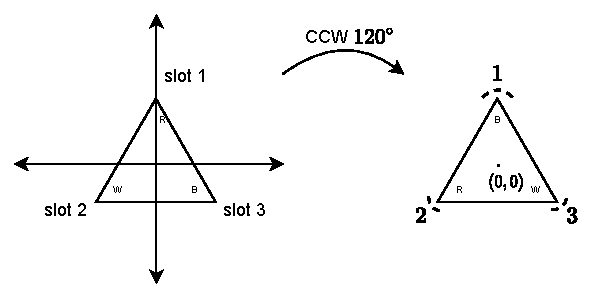
\includegraphics[width=0.75\textwidth]{Figures/Dihedral Group Example_1.pdf}

\hspace{-0.5in}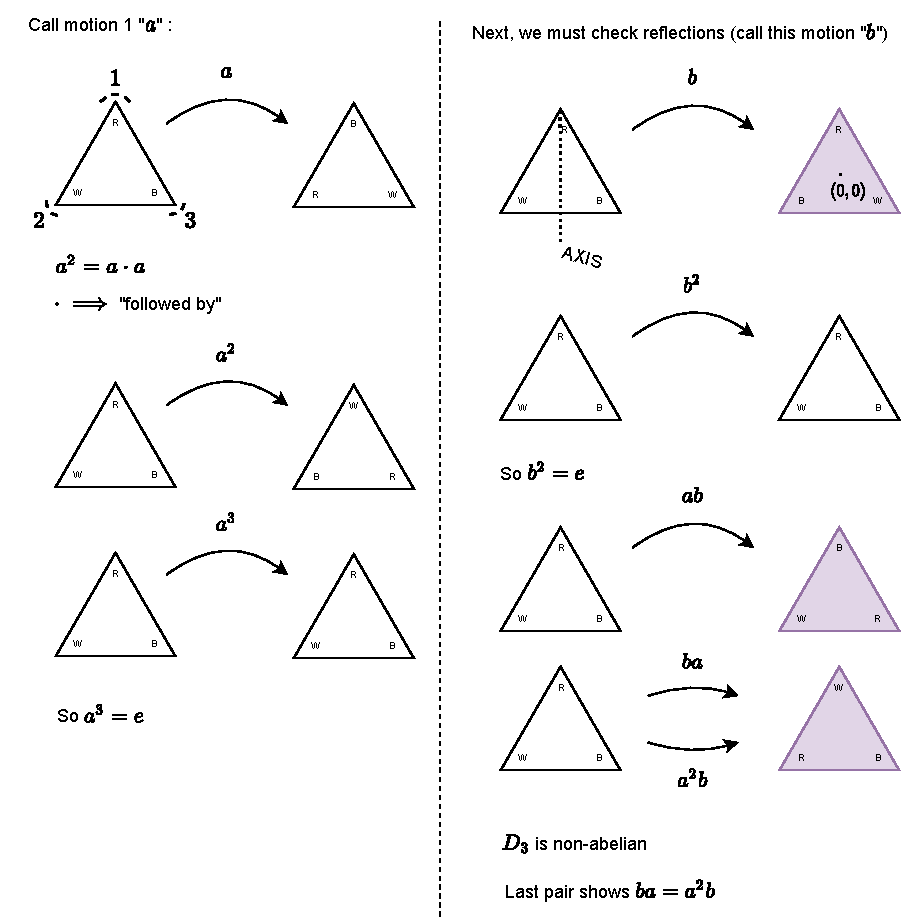
\includegraphics[width=1.1\textwidth]{Figures/Dihedral Group Example_2.pdf}\\
\begin{align}
    D_3&= \{e,a,a^2,b,ba,ab\} \nonumber \\
    &= \langle \underbrace{a}_{*},\underbrace{b}_{**} \rangle \nonumber \\
    &* - \text{ Rotation through }120^\circ \text{ CCW.} \nonumber \\
    &** - \text{ Flip through axis.} \nonumber
\end{align}
$D_3$ has the following set of minimal relations
\begin{align}
    a^3&=e \nonumber \\
    b^2&=e \nonumber \\
    ba&=a^2b \nonumber 
\end{align}
\end{example}

\subsection*{$D_n$ -- Main Facts}
\begin{enumerate}
    \item $D_n$ is generated by $\langle a,b \rangle$ where $a$ is a CCW rotation about origin of $\frac{360}{n}$ degrees, $b$ is reflection about a line through $(0,0)$ so that when you reflect it will carry $n-$gon to itself, (have $n$ choices for choosing axis for $b$)\\
    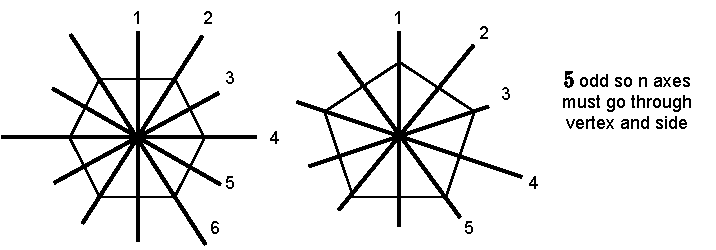
\includegraphics[width=0.65\textwidth]{Figures/AxisChoiceforB-Dihedral.pdf}
    \item $D_n$ is completely determined by its generators and the relations:
    \begin{align}
        a^n&=e\nonumber \\
        b^2&=e \nonumber \\
        ba&=a^{n-1}b \nonumber
    \end{align}
    \item $o(D_n)=2n$ the elements are:
    \begin{align}
        &a,a^2,a^3, ... , a^{n-1},e \nonumber \\
        &b,ab,a^2b, ... , a^{n-1}b \nonumber
    \end{align}\\
    These elements give a closed system...
    \item There is a non-abelian group of every even order $> 4$.
 
    \begin{tabular}{|c|c|c|c|c|c|} \hline
            Order: & 6&8&10&12&14   \\
             Group: &$D_3$ &$D_4$&$D_5$&$D_6$&$D_7$ \\ \hline 
    \end{tabular}
    
    Note $D_7$ corresponds to the symmetries of a "heptagon" $\smiley{}$. Also note that since $o(D_3)=6$ then by Lagrange, if $H < D_3 \ \implies o(H)$ can be $1,\underbrace{2,3}_{\text{primes}}$ or $6$. \steezybreak\\
    Lagrange Cor \#5: groups of prime order are cyclic. \\
    \begin{align}
        \{\underset{1}{e},\underset{3}{a},\underset{3}{a^2},\underset{2}{b},\underset{2}{ab},\underset{2}{a^2 b}\} \nonumber
    \end{align}
    $4$ non-trivial subgroups. \\
    \begin{tabular}{c|cccccc} 
            $D_3$ & $e$ & $a$ & $a^2$& $b$ & $ab$ & $a^2 b$   \\ \hline 
            $e$ & $e$ & $a$ & $a^2$& $b$ & $ab$ & $a^2 b$   \\  
            $a$ & $a$ & $a^2$ & $e$& $ab$ & $a^2 b$ & $b$   \\ 
            $a^2$ & $a^2$ & $e$ & $a$& $a^2 b$ & $b$ & $ab$   \\  
            $b$ & $b$ & $a^2 b$ & $ab$& $e$ & $a^2$ & $a$   \\  
            $ab$ & $ab$ & $b$ & $a^2b$& $a$ & $e$ & $a^2$   \\  
            $a^2 b$ & $a^2 b$ & $ab$ & $b$& $a^2$ & $a$ & $e$   \\  
    \end{tabular}
\end{enumerate}
\steezybreak
\begin{tcolorbox}
    \begin{center}
        $\star\star\star$ \textbf{Read up to this point to Complete Homework 6 (Located in \ref{sec:HW6})} $\star\star\star$
    \end{center}
    \end{tcolorbox}
\steezybreak
\section{Cayley's Theorem}
Arthur Cayley (1821-1895) -- set down modern definition of Groups. He was a total G-daddy dog. Used to be a lawyer, Cambridge picked him up to work in Mathematics.

\subsection*{Automorphic bijections as permutations}
Suppose $S$ is a set with $n$ elements. A bijection of $S$ to itself can be viewed as a permutation of the elements of $S$. Recall $S_3=\{\text{bijections on a set of $3$ elements.}\}$\steezybreak\\
Element $\sigma\tau$ in $S_3$ was this bijection:\\
\begin{center}
    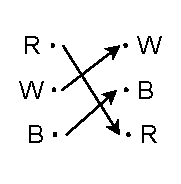
\includegraphics[width=0.3\textwidth]{Figures/Permutations_Cayley_1.pdf} 
\end{center}
So $\sigma \tau$ permutes $RWB \rightarrow WBR$\\
\begin{align}
    S_3= \{\underset{I}{RWB},\underset{\sigma}{RBW},\underset{\tau}{BWR},\underset{\sigma\tau}{WBR},\underset{\tau\sigma}{BRW},\underset{\sigma\tau\sigma}{WRB}\} \nonumber
\end{align}
In general, $S_n= \{\text{Permutations on $n$ elements}\}$ is a group under composition with $o(S_n)=n!$, as we noted before, $S_n$ can alternatively be called $A(S)$ (automorphisms), this name is usually reserved for cases where $S$ has infinite members/elements.
\newpage

\begin{theorem}[Cayley's Theorem] 
Every group $G$ is isomorphic to a subgroup of $A(G)$.
\begin{itemize}
    \item In other words: Every group has the structure of some permutation group.
    \item So permutation groups contain all possible group structure.
\end{itemize}
%(for finite $G$) (idk if that's true, any group can act on itself by left product and this is exactly how we define tau and then psi... I believe this proof holds for any G! (finite or infinite!) although the beginning of part 1's explanation is easier to think of in terms of finite G... but nothing stops you from imagining an infinite cayley table and the "b-row" intuition doesn't stop us from constructing a well-defined mapping \tau_g for each (even infinitely many ) g \in G!
\textit{Proof:} 
\begin{enumerate}
   \item Each row in the Cayley table for $G$ is a permutation of $G$'s elements and each permutation produces a bijection from $G\rightarrow G$.\\%$\blacksquare$ \steezybreak\\
\hrule
%Boy that was quick... how about an example to crystallize the argument above...\steezybreak\\
\textbf{Example:} $b$-row of Cayley table gives $y$ values for the map "L-multiply by $b$"
\begin{align}
    &\tau_b : G\rightarrow G \nonumber \\
    &\tau_b(x)=bx \ \forall \ x \in G \nonumber 
\end{align}
\hrule
Now,
\begin{align}
    \forall \ g\in G, \text{ define } &\tau_g: G\rightarrow G \nonumber \\
    \text{by }&\tau_g(x)=gx \ \forall \ x \in G. \nonumber
\end{align}
\textit{Claim:} $\tau_g$ has an inverse, namely $\tau_{g^{-1}}$\\
\textit{Proof:} $x\in G$
\begin{align}
    (\tau_{g^{-1}} \circ \tau_g)(x)&=\tau_{g^{-1}}(gx)=g^{-1}gx=ex=x \nonumber \\
    (\tau_g \circ \tau_{g^{-1}})(x)&=\tau_{g}(g^{-1}x)=gg^{-1}x=ex=x \nonumber \\
    \therefore (\tau_{g^{-1}} \circ \tau_g) &= I_G \text{ and } (\tau_g \circ \tau_{g^{-1}})= I_G \nonumber \\
    \therefore \tau_g &\text{ has and inverse.} \nonumber \\
    \therefore \tau_g &\text{ is a bijection by Lemma 1.2.3} \nonumber
\end{align}
So $\tau_g \in A(G)$
\item Define $\psi:G\rightarrow A(G)$ by $\psi(g)=\tau_g \ \forall \ g\in G$ \\
$\psi$ is a homomorphism: 
\begin{align}
    &g,g' \in G \nonumber \\
    &\begin{rcases}
    \psi(g\cdot g')=\tau_{gg'}  \\
    \psi(g)\cdot \psi(g')=\tau_{g}\underset{\text{in }A(G)}{\cdot} \tau_{g'} \ \ \ \ 
    \end{rcases}\text{Are these the same?} \nonumber
\end{align}
Take $x\in G$
\begin{align}
    \tau_{gg'}(x)&=gg'x \nonumber \\
    (\tau_g\circ \tau_{g'})(x)&= \tau_g(\tau_{g'}(x))=\tau_g(g'x)=gg'x \nonumber \\
    &\therefore \tau_g\circ\tau_{g'}=\tau_{gg'} \nonumber \\
    &\therefore \psi(gg')=\psi(g)\cdot \psi(g') \nonumber \\
    &\therefore \psi \text{ is a homomorphism.} \nonumber
\end{align}
$\psi$ Injective: Take $g\neq h $ in $G$
\begin{align}
    &\begin{rcases}
    \psi(g)=\tau_g 
    \psi(h)=\tau_h
    \end{rcases} \text{ must show }\tau_g\neq \tau_h \nonumber
\end{align}
Let's see where $e$ gets mapped under $\tau_g$ and $\tau_h$.
\begin{align}
    \tau_g(e)&=ge=g \nonumber \\
    \tau_h(e)&=he=h \nonumber \\
    &\therefore \tau_g(e)\neq \tau_h(e) \nonumber \\
    &\therefore \tau_g \neq \tau_h \nonumber
\end{align}
So $\psi$ is injective. \\
Lastly, we replace $A(G)$ with the image $\psi(G)$ to make $\psi$ surjective
\begin{align}
    &\psi: G\rightarrow \psi(G) \nonumber \\
    &\psi(g)=\tau_g \ \ \ \ \ \ \ \ \text{ (revised defn.)} \nonumber
\end{align}
$\therefore G \ \ \ \overset{\psi}{\approx} \underset{\text{a subgroup of }A(G)}{\psi(G)}. \ \ \ \ \blacksquare$
\end{enumerate}

\end{theorem}

\section{Permutation Groups}
To begin we would like to streamline the notation for permutations... Consider the following diagram\\
\begin{center}
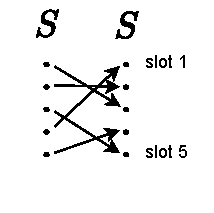
\includegraphics[width=0.25\textwidth]{Figures/Permutation_Notation_ex.pdf}
\end{center}
We will denote this map by $\begin{pmatrix} 1&2&3&4&5\\ 3&2&5&1&4
\end{pmatrix}$ This means 1 goes to 3, 2 goes to 2, 3 goes to 5 and so on.\\
Recall that $S_5$ has order $5!=60$ and now suppose in $S_5$ that 
\begin{align}
    \sigma = \begin{pmatrix}
    1&2&3&4&5\\1&2&4&3&5
    \end{pmatrix} \nonumber \\
    \tau = \begin{pmatrix}
    1&2&3&4&5 \\ 2&4&1&5&3
    \end{pmatrix} \nonumber
\end{align}
We can represent the "product" of these two maps via their composition:
\begin{align}
    \sigma \cdot \tau &= \begin{pmatrix}
    1&2&3&4&5 \\ 1&2&4&3&5
    \end{pmatrix}\begin{pmatrix}
    1&2&3&4&5 \\ 2&4&1&5&3
    \end{pmatrix}\nonumber \\
    &= \begin{pmatrix}
    1&2&3&4&5 \\
    2&4&5&1&3
    \end{pmatrix} \ \ \ \ \ \ \ \ \text{(Thread through maps)} \nonumber
\end{align}


A perceptive reader might notice that this composition is a little different from how we wrote composition before. Normally, we would consider $\sigma \cdot \tau$ to correspond to sigma after tau meaning we should thread through tau then through sigma, however we adopt a notational change that mirrors the original notation of Herstein for composing maps (that is $\sigma \cdot \tau$ should be read as sigma then tau in this section). We use this convention in this section because it makes it easier to read from left to right, threading through consecutive maps.

Now then, with $\sigma$ defined as above, what is the order of $\sigma$ in $S_5$?
\begin{align}
    \sigma^2&=\begin{pmatrix}
    1&2&3&4&5 \\ 1&2&4&3&5
    \end{pmatrix}\begin{pmatrix}
    1&2&3&4&5 \\ 1&2&4&3&5
    \end{pmatrix} = \begin{pmatrix}
    1&2&3&4&5 \\ 1&2&3&4&5
    \end{pmatrix} = e \in S_5 \nonumber \\
    &\therefore \ \ o(\sigma)=2 \nonumber
\end{align}
What is the inverse of $\tau$ defined above?
\begin{align}
    \tau^{-1}= \begin{pmatrix}
    1&2&3&4&5 \\ 3&1&5&2&4
    \end{pmatrix}\nonumber
\end{align}
It is simple to confirm that the above map corresponds to $\tau$'s unique inverse, and in general we can construct inverse map for a map $\tau$ by sending the second row of $\tau$ back to it's first row (notice how $\tau$ sends 1 to 2 and 2 to 4, ... so in order to undo tau we just send 2 to 1, 4 to 2, and so on.)

Let $S$ be a set with $n$ elements and take $\theta \in S_n$, we'll use powers of $\theta$ to define an equivalence relation on $S$. Define the relation $\equiv_{\theta}$ by:
\begin{align}
    a\equiv_{\theta} b \iff \exists i \in \Z \ni b= \theta^i(a) \nonumber
\end{align}

\begin{example}
Consider $S=\{1,2,3,4,5\}$ and
\begin{align}
    \theta = \begin{pmatrix}
    1&2&3&4&5 \\ 5&1&4&3&2
    \end{pmatrix} = (1,5,2)(3,4)\nonumber
\end{align}
Under $\theta$, which elements $b\in S$ are related to $2$?
\begin{align}
    2\equiv_{\theta} b \iff b=\theta^i(2) \ \text{for } i \in \Z \nonumber
\end{align}
Let's have a look at $\theta^i(2)$
\begin{align}
    \theta^0(2)&=2 \nonumber \\
    \theta^1(2)&=1 \nonumber \\
    \theta^2(2)&=5 \nonumber \\
    \theta^3(2)&=2 \nonumber \\
    \text{Negative Powers:} \nonumber \\
    \theta^{-1}(2)&=5 \nonumber \\
    \theta^{-2}(2)&=1 \nonumber \\
    \theta^{-3}(2)&=2 \nonumber
\end{align}
So $b\equiv_{\theta}\theta^i(2)= \{1,2,5\}$, $2, 1$, and $5$ are related to $2$ under $\equiv_{\theta}$
\end{example}
\textbf{Claim:} $\equiv_{\theta}$ is an equivalence relation on $S$. \\
\textit{Proof:}
\begin{enumerate}
    \item \textbf{Reflexive:} $\forall \ a \in S$, $a\equiv_{\theta} a $ because $\theta^0(a)=a$ (applying the theta map 0 times to element a is just element a)
    \item \textbf{Symmetric:} For $a,b \ \in S$ assume that $a\equiv_{\theta} b$, then $\exists \ i \in \Z \ni \ b=\theta^i(a)$, now since $\theta^i \in S_n$, its inverse $[\theta^i]^{-1}\in S_n$, $[\theta^i]^{-1}=\theta^{-i}$. So $\theta^{-i}(b)= \theta^{-i}[\theta^i(a)] = \theta^{-i}\cdot \theta^i(a)=\theta^0(a)=a$, since $a=\theta^{-i}(b)$ and $-i\in \Z$, $b\equiv_{\theta} a$.
    \item \textbf{Transitivity: }Let $a, b, c \ \in S$ and assume $a\equiv_{\theta} b$ and $b\equiv_{\theta} c$,
    \begin{align}
        a&\equiv_{\theta} b \implies \  \exists \ i \in \Z \ni b= \theta^i(a)\nonumber \\
        b&\equiv_{\theta} c \implies \  \exists \ j \in \Z \ni c= \theta^j(b)\nonumber \\
        c&= \theta^j(b)=\theta^j(\theta^i(a))=\theta^{i+j}(a) \nonumber \\
        &\therefore \ \exists \  n=i+j \in \Z \ni c=\theta^n(a) \nonumber \\
        &\therefore \ a \equiv_{\theta} c \nonumber \\
        &\therefore \ \equiv_{\theta} \text{ is transitive.} \ \ \blacksquare \nonumber
    \end{align}
\end{enumerate}
So $\equiv_{\theta}$ partitions $S$ into disjoint equivalence classes. For this relation, these equivalence classes are called ``orbits".

\begin{example}
$\theta= \begin{pmatrix}
1&2&3&4&5 \\ 5&1&4&3&2
\end{pmatrix}$ \\
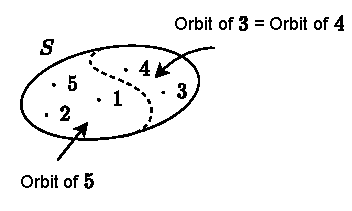
\includegraphics[width=0.6\textwidth]{Figures/Orbits_ex.pdf}\\
A \textit{cycle} is an orbit which is arranged to show the sequence in which  elements are picked up.
\begin{align}
    \text{Orbit of } 2 &= \{1,2,5\} \nonumber \\
    \text{Cycle of } 2 &= (\underset{\longleftarrow}{2^{\rightarrow},1^{\rightarrow},5}) \ \ \ 2 \text{ gets mapped to }1, 1 \text{ gets mapped to } 5, 5 \text{ gets mapped to } 2 \nonumber
\end{align}
The map $\theta$ in this example can be decomposed into a composition of a 3-cycle and a 2-cycle
$(2,1,5)=(1,5,2)=(5,2,1)$ 3-cycle(s) \\
$(3,4)=(4,3)$ 2-cycle.
\end{example}
\begin{definition}[m-cycle]
Let $\theta \in S_n$, $a\in S$\\
\begin{align}
    (a,\theta(a),\theta^2(a), \dots, \theta^m(a))\nonumber
\end{align}
Where $\theta^m(a)=a$ is an \textit{m-cycle} of $S_n$. Here, $m$ denotes the length of the cycle.
\end{definition}
\begin{example}

\begin{align}
\theta &= \begin{pmatrix}
1&2&3&4&5\\5&1&4&3&2
\end{pmatrix}  \nonumber \\
&= (1,5,2)(3,4) \nonumber
\end{align}
So $\theta$ can be written as a product (composition, i.e. ``followed by") of cycles
\end{example}
\begin{example}
\begin{align}
    \theta &= \begin{pmatrix}
1&2&3&4&5&6&7&8 \\
2&7&5&4&6&8&1&3
\end{pmatrix} \nonumber \\
&= (1,2,7)(3,5,6,8)(4) \nonumber
\end{align}
\end{example}
\begin{lemma}
Every permutation has a unique decomposition as a product of disjoint cycles. \\
\textit{Proof:} The sequence of integers in the cycles is determined by the permutation (i.e. a decomposition exists). The sequence can be determined in one way only (it's unique because it's a bijection). The cycles are equivalence classes under the relation $\equiv_{\text{perm}}$ so they are disjoint; their composition (product) is the same bijection as the permutation. $\blacksquare$
\end{lemma}
\begin{example}
Consider the following elements of $S_6$,
\begin{align}
    \theta= \begin{pmatrix}
    1&2&3&4&5&6 \\ 3&5&1&2&4&6
    \end{pmatrix}, \ \ \tau = \begin{pmatrix}
    1&2&3&4&5&6 \\ 2&1&6&5&3&4
    \end{pmatrix} \nonumber
\end{align}
Now let's find the cycle decomposition of $\tau \theta$
\begin{align}
    \theta &= (1,3)(2,5,4)(6)\nonumber \\
    \tau &= (1,2)(3,6,4,5) \nonumber \\
    \tau\theta &= (1,2)(3,6,4,5)(1,3)(2,5,4)(6) \ \ \ \ (\text{Note that }(1,2) \text{ and } (1,3) \text{ are not disjoint, so we must reduce)} \nonumber \\
    &=(1,5)(2,3,6)\centernot{{(4)}} \ \ \ \ \leftarrow \text{ Customary to Eliminate 1-cycles (they go to themselves)} \nonumber
\end{align}
We arrive at the final expression by noting
\begin{align}
    1 \overset{\text{1st}}{\rightarrow} 2 \overset{\text{2nd}}{\rightarrow} 2 \overset{\text{3rd}}{\rightarrow}2 \overset{\text{4th}}{\rightarrow}5 \overset{\text{5th}}{\rightarrow} 5 \nonumber \\
    2 \overset{\text{1st}}{\rightarrow} 1 \overset{\text{2nd}}{\rightarrow} 1 \overset{\text{3rd}}{\rightarrow}3 \overset{\text{4th}}{\rightarrow}3 \overset{\text{5th}}{\rightarrow}3 \nonumber \\
    3 \overset{\text{1st}}{\rightarrow} 3 \overset{\text{2nd}}{\rightarrow} 6 \overset{\text{3rd}}{\rightarrow}6 \overset{\text{4th}}{\rightarrow}6 \overset{\text{5th}}{\rightarrow}6 \nonumber \\
    4 \overset{\text{1st}}{\rightarrow} 4 \overset{\text{2nd}}{\rightarrow} 5 \overset{\text{3rd}}{\rightarrow}5 \overset{\text{4th}}{\rightarrow}4 \overset{\text{5th}}{\rightarrow}4 \nonumber \\
    5 \overset{\text{1st}}{\rightarrow} 5 \overset{\text{2nd}}{\rightarrow} 3 \overset{\text{3rd}}{\rightarrow}1 \overset{\text{4th}}{\rightarrow}1 \overset{\text{5th}}{\rightarrow}1 \nonumber \\
    6 \overset{\text{1st}}{\rightarrow} 6 \overset{\text{2nd}}{\rightarrow} 4 \overset{\text{3rd}}{\rightarrow}4 \overset{\text{4th}}{\rightarrow}2 \overset{\text{5th}}{\rightarrow}2 \nonumber
\end{align}
Where 1st-5th denote the application of cycles 1 through 5 of the non-reduced expression. We can see that the total effect of the non-reduced expression is the composition of disjoint cycles (1,5) and (2,3,6). Since there are only 6 elements to consider, it is often possible to find the unique disjoint decomposition without having to thread through \textit{each and every} element (e.g. we did not need to see where 6 went because it only had one slot it could land in, the 2 slot.)
\end{example}

\begin{example}
\textbf{Problem:} Suppose $\theta = (1,3,9)(2,4,8,5)(6,10,7)\in S_{10}$. Find the order of $\theta \in S_{10}$. \steezybreak\\
We first note that $S_{10}$ has order $10!=3,628,800$, so counting powers might not be the most efficient approach... let's take a brief detour to think about the order of a cycle... \steezybreak\\
\textbf{Aside:} What's the order of an $m$-cycle?
\begin{align}
    (s,t,u,v,w) \nonumber
\end{align}
In this arbitrary 5-cycle, each element is sent one slot to the right, so
\begin{align}
    (s,t,u,v,w)^2 &= (s,t,u,v,w)(s,t,u,v,w)\nonumber \\
    &= (s,u,w,t,v) \nonumber
\end{align}
since $s$ will be taken to the $t$ slot after the first application and $t$ slot gets taken to $u$ slot after the second application; similarly, $u$ gets taken to the $v$ slot after the first application and $v$ slot gets taken to the $w$ slot after the second application. Let's try cubing
\begin{align}
    (s,t,u,v,w)^3&=(s,t,u,v,w)(s,t,u,v,w)(s,t,u,v,w) \nonumber \\
    &= (s,v,t,w,u) \nonumber
\end{align}
So, for $n$ power, cycle shifts each element $n$ spaces
\begin{align}
    (s,t,u,v,w)^5=I=(s)(t)(u)(v)(w)\nonumber
\end{align}
If power is $r$, the resulting cycle sends each element $r$ slots to the right. We conclude that the order of an $m-$cycle is the length of the cycle, $m$. \steezybreak\\
Back to the problem... What's the order of $\theta \in S_{10}$? It should be the smallest $k\in \Z$ so that $\theta^k= I = e \in S_{10}$
\begin{align}
    \theta^k&=[(1,3,9)(2,4,8,5)(6,10,7)]^k \nonumber \\
    &= \underbrace{(1,3,9)^k}_{\text{order }3}\underbrace{(2,4,8,5)^k}_{\text{order }4}\underbrace{(6,10,7)^k}_{\text{order }3} \nonumber
\end{align}
Note, any common multiple of $3$ and $4$ will send each cycle to $I$, $k$ should be the \textit{least} common multiple. So $k=LCM(3,4)=12$.
\end{example}

In general, if $\theta\in S_{n}$ then $o(\theta)= LCM(\text{lengths of disjoint cycles in the decomposition of }\theta)$
\begin{definition}[Transposition]
A \textit{transposition} is a 2-cycle. Consider the cycle $(a_1,a_2)$,
\begin{center}
    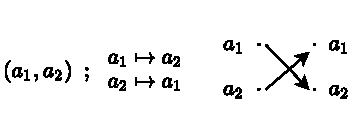
\includegraphics[width=0.4\textwidth]{Figures/transposition_2cycle.pdf}
\end{center}
All other elements are sent to themselves under $(a_1,a_2)$.
\end{definition}

\begin{lemma}
Every permutation can be written as a product of transpositions. \steezybreak\\
\textit{Proof:} By Lemma 2.10.1, it is enough to prove this can be done on cycles, consider an arbitrary $n$-cycle:
\begin{align}
    (a_1, \dots, a_n)=(a_1,a_2)(a_1,a_3)(a_1,a_4)\dots(a_1,a_n). \ \ \blacksquare \nonumber
\end{align}
\end{lemma}
\textbf{NOTE}, the product of transpositions promised by this lemma is \textul{\textbf{NOT}} unique, BUT the number of transpositions involved will either always be \textul{even} or always be \textul{odd} (technical proof omitted, see pg. 79 of Herstein or Theorem 2.1 \href{https://kconrad.math.uconn.edu/blurbs/grouptheory/sign.pdf}{here})
%% Proof that Parity is well-defined (every decomposition into 2-cycles of a permutation \sigma is either always odd or always even )

% Permutation Parity is Well-defined: Given any two representations of $\sigma \in S_n$ as a product of transpositions $\sigma = \tau_1\tau_2 · · · \tau_r = \tau_1' \tau_2' · · · \tau_{r'}' $. Then $r \equiv r' mod 2$ (i.e. $r$ and $r'$ are either both even or both odd). \textit{Proof:} Using the two products of transpositions that equal $\sigma$ above we can express the identity permutation as a product of $r + r'$ transpositions: $(1) = \sigma\sigma^{-1} = \tau_1\tau_2 · · · \tau_r\tau_{r'}'\tau_{r'−1}'· · · \tau_1'.$ (Note $\tau^{−1} = \tau$ for transpositions $\tau$ and inverting a product reverses the order of multiplication.) 

% Claim: A product of transpositions equal to (1) must have an even number of transpositions. This claim forces $r + r '$ above to be even, so $r ≡ r ' mod 2$. To prove the claim, write the identity in $S_n$ as a product of $k$ transpositions: $(1) = (a1b1)(a2b2)· · ·(akbk)$, where $k \geq 1$ and $ai \neq bi$ for all $i$. We want to show $k$ is even and will induct on $k$. The product on the right side of (2.2) can’t have k = 1 since a transposition is not (1). We could have k = 2, which is even. Suppose, by induction, that k ≥ 3 and every product of fewer than k transpositions that equals (1) has an even number of transpositions. Some transposition (aibi) for i 6= 1 has to move a1 (otherwise the overall product on the right side of (2.2) sends a1 to b1, which is not the identity permutation). So a1 must be an ai or bi for i > 1. We can suppose a1 is ai since (aibi) = (biai). The two equations (cd)(ab) = (ab)(cd), (bc)(ab) = (ac)(bc), where different letters are different numbers, show a product of two transpositions where the second one moves a and the first one does not can be rewritten as a product of two transpositions in which the first one moves a and the second one does not. So in (2.2), without changing the number of transpositions we can arrange for a transposition moving a1 other than (a1b1) to appear directly after (a1b1): we can assume a2 = a1. Now consider the cases b2 = b1 and b2 6= b1. Case 1: b2 = b1. The product (a1b1)(a2b2) in (2.2) is (a1b1)(a1b1), which is the identity and can be removed. This turns the right side of (2.2) into a product of k−2 transpositions. By induction, k − 2 is even so k is even. Case 2: b2 6= b1. Check (a1b1)(a2b2) in (2.2), which is (a1b1)(a1b2), can be written as (a1b2)(b1b2) since a1, b1, and b2 are all different. Then (2.2) can be rewritten as (2.3) (1) = (a1b2)(b1b2)(a3b3)· · ·(akbk), where only the first two transpositions have been changed. Now run through the above argument with (2.3) in place of (2.2). It involves the same number k of transpositions, but THE SIGN OF A PERMUTATION 3 there are fewer transpositions in (2.3) that move a1 since we used to have (a1b1) and (a1b2) in the product and now we have (a1b2) and (b1b2).2 Some transposition in (2.3) other than the first term (a1b2) moves a1, so by running through the above argument with (2.3) in place of (2.2) we land in either Case 1, which lets us drop the number of transpositions by 2 and we’re done by induction, or Case 2, which lets us drop the number of transpositions moving a1 by 1 without changing the total number of transpositions. When (1) is a product of transpositions with the leftmost one moving a1, there is always at least one more transposition in the product moving a1 and Case 2 reduces that number by 1. So in finitely many steps we have to land in Case 1 and then we are done. $\blacksquare$




\begin{example}
We illustrate the \textit{non-uniqueness} of the 2-cycle (transpositions) decomposition from the lemma above (Lemma 2.10.2) with a simple example:
\begin{center}
    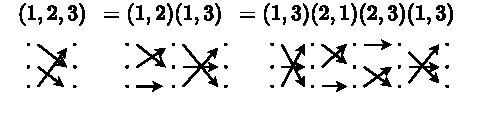
\includegraphics[width=0.75\textwidth]{Figures/non_unique_cycle_trans.pdf}
\end{center}
\end{example}
\begin{definition}[Parity of Permutations]
A permutation $\theta \in S_n$ is \textit{even}, or alternatively \textit{odd}, if it breaks down into an even, or alternatively odd, number of transpositions. The state of $\theta$ as ``even" or ``odd" is called the \textit{parity} of $\theta$.
\end{definition}

\begin{example}
Find the order and parity of $\theta = (1,2,8)(2,4)(3,10,9)(4,7,6)$

\begin{enumerate}
    \item \textbf{Order:} Get disjoint cycles first:
    \begin{align}
        \theta = (1,7,6,4,2,8)(3,10,9)\centernot{(5)}\nonumber
    \end{align}
    So $o(\theta)=LCM(3,6)=6$
    \item \textbf{Parity:} Now let's write the disjoint cycles as a product of 2-cycles:
    \begin{align}
        \theta=(1,7)(1,6)(1,4)(1,2)(1,8)(3,10)(3,9) \nonumber
    \end{align}
    Since we can decompose $\theta$ into $7$ 2-cycles, $\theta$ is an odd permutation.
\end{enumerate}
\end{example}

\begin{example}
What is the parity of $I$, the identity map, which serves as $e\in S_n$?
\begin{align}
    I&=(1)(2)(3)\dots (n) \nonumber \\
    &= (1,2)(2,1)(1,3)(3,1)(1,4)(4,1)\dots (1,n)(n,1) \nonumber
\end{align}
We have $2(n-1)$ transpositions, an even number.\\
$\therefore$ $I$ is an even permutation.
\end{example}

\begin{lemma}
$n\in \Z$, $n\geq 2$. Suppose $A_n$ is the subset of $S_n$ consisting of all even permutations in $S_n$. Then
\begin{align}
    A_n \triangleleft S_n \ \ \text{and} \ \ \  o(A_n)=\frac{n!}{2}\nonumber
\end{align} \\
\noindent \textit{Proof:} We will begin by showing $A_n < S_n$ then we will show $A_n\triangleleft S_n$ and finally we will show $o(A_n)=o(S_n)/2 = n!/2$. \steezybreak\\
$\boxed{A_n < S_n}$ We first note that $I\in A_n$ because it is an even permutation, so we can use Lemma 2.4.2 because $S_n$ is finite ($o(S_n)=n!$). Thus, we need only show that $A_n$ is closed. \steezybreak \\ 
Take $\sigma, \tau \in A_n$, $\sigma$ and $\tau$ are both even permutations.
\begin{align}
    &\sigma \text{ even }\implies \sigma \text{ decomposes into }2k \text{ transpositions for } k\in \Z \nonumber \\
    &\tau \text{ even }\implies \tau \text{ decomposes into }2l \text{ transpositions for } l\in \Z \nonumber \\
    &(\sigma \cdot \tau) = (\text{trans. of }\sigma)(\text{trans. of }\tau)\nonumber \\
    &\therefore \sigma\tau \text{ decomposes into }2k+2l \text{ transpositions} 2(k+l), \ (k+l)\in \Z \nonumber \\
    &\therefore \sigma \tau \text{ is even parity} \nonumber \\
    &\therefore \sigma \tau \in A_n. \ A_n\text{ is closed.} \nonumber \\
    &\therefore A_n < S_n. \nonumber
\end{align}\\
\noindent $\boxed{A_n \triangleleft S_n}$ Now we'll show $A_n$ is the kernel of a homomorphism and $A_n \triangleleft S_n$ will follow by Lemma 2.7.3. \steezybreak\\
Define $\psi : S_n \rightarrow \{-1,1\} \text{ under multiplication}$ (tiny group) its Cayley table looks like this 
\begin{tabular}{r|rr}
$\cdot$ & $1$  & $-1$ \\ \hline
$1$     & $1$  & $-1$ \\
$-1$    & $-1$ & $1$ 
\end{tabular}\\
by the following mapping: $\forall \sigma \in S_n \ \ \psi(\sigma)= \begin{cases}
  \ \ 1 \text{ if even} \\
  -1\text{ if odd}
\end{cases}$\\

\noindent Now, to show $\psi$ is a homomorphism we must show $\psi(\sigma\tau)=\psi(\sigma)\psi(\tau) \ \forall \ \sigma,\tau\in S_n$. \\
\noindent First we note 
\begin{align}
    \psi(\sigma\tau) &= \begin{cases}
      \ \ 1 \text{ if $\sigma\tau$ is even} \\
      -1\text{ if $\sigma\tau$ is odd} 
    \end{cases} \nonumber
\end{align}
Now we consider the cases for parity of $\sigma$ and $\tau$:
\begin{align}
    even-even: \ \ \ \psi(\sigma)\psi(\tau)=1\cdot 1 = 1 \nonumber \\
    odd-odd: \ \ \ \psi(\sigma)\psi(\tau)=-1 \cdot -1 = 1 \nonumber \\
    odd-even: \ \ \ \psi(\sigma)\psi(\tau)=-1\cdot 1 = -1 \nonumber \\
    even-odd: \ \ \ \psi(\sigma)\psi(\tau)=1\cdot -1 - -1 \nonumber
\end{align}
So $\psi$ is a homomorphism. Now we note 
\begin{align}
    \ker\psi &= \{\sigma \in S_n | \psi(\sigma) = 1\} \nonumber \\
    &=\{\text{even permutations}\} \nonumber \\
    &= A_n \nonumber
\end{align}
Since $A_n$ is the kernel of a homomorphism from $S_n$ into another group, $A_n \triangleleft S_n$ (L 2.7.3). \\
\noindent $\boxed{o(A_n)=n!/2}$ To show the final result we recall the First Isomorphism theorem and Lemma 2.6.4. 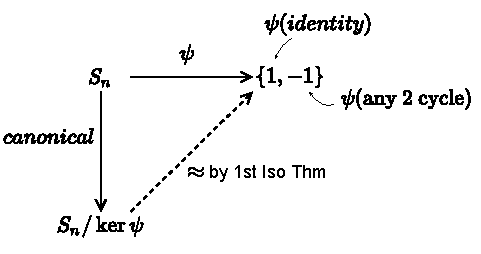
\includegraphics[]{Figures/Lem2-10-3.pdf} \\
Since we can produce pre-images for both -1 and 1, $\psi$ is a surjection and so $S_n/ker\psi$ is isomorphic to $\{-1,1\}$ by the 1st Isomorphism theorem. Therefore $o(S_n/A_n)= 2$. Applying L 2.6.4 we have $o(S_n)/o(A_n)=2 \ \implies \ o(A_n)=n!/2. \ \ \ \blacksquare $
\end{lemma}
\begin{definition}[Alternating Group]
$A_n$ from Lemma 2.10.3 is the \textit{Alternating Group} of degree $n$
\end{definition}

\subsubsection{Importance of Alternating Groups (Example 1)}
Consider the following conjecture, which is the converse of Lagrange's thm: If $m\in \Z^+ \ni \ m | o(G)$, then $G$ has a subgroup of order $m$.  \steezybreak \\
Is this true or false? FALSE!\\ 
$A_4$ shows this is false because $o(A_4) = 4!/2 = 12$ but $A_4$ has no subgroup of order 6!\\
\noindent \textit{Proof:} Suppose $A_4$ has a subgroup of order 6, call it $H<A_4$.\\
$i_{A_4}(H)=2 \ \implies \ H\triangleleft A_4$. Let's figure out the elements of $A_4$, we'll consider elements in $S_4$ to find those in $A_4$.
\begin{itemize}
    \item \textul{4-cycles} $(a,b,c,d)=(a,b)(a,c)(a,d)$, odd $\not\in A_4$
    \item \textul{Product of 2-cycles} $(a,b)(c,d)$  EVEN $\in A_4$
    \item \textul{3-cycles} $(a,b,c) = (a,b)(a,c)$ EVEN $\in A_4$
\end{itemize}
$S=\{1,2,3,4\}$. So $A_4$ has 12 elements, we first look at the order 2 elements
\begin{align}
    (1,3)(2,4) \nonumber \\
    (1,2)(3,4) \nonumber \\
    (1,4)(2,3) \nonumber
\end{align}
Then the order 3 elements
\begin{align}
    (2,3,4) \ \ \ (1,3,4) \ \ \ (1,2,4) \ \ \ (1,2,3)\nonumber \\
    (2,4,3) \ \ \ (1,4,3) \ \ \ (1,4,2) \ \ \ (1,3,2)\nonumber
\end{align}
% \begin{align}
%     (2,3,4) \nonumber \\
%     (2,4,3) \nonumber \\
%     (1,3,4) \nonumber \\
%     (1,4,3) \nonumber \\
%     (1,2,4) \nonumber \\
%     (1,4,2) \nonumber \\
%     (1,2,3) \nonumber \\
%     (1,3,2) \nonumber \\
% \end{align}
Notice how the order 3 elements come in pairs $\alpha, \alpha^2$ e.g. $(1,2,3)= \alpha$ and $(1,3,2) = \alpha^2$ \\
Lastly $A_4$ has a single element of order 1, $(1)(2)(3)(4)$. \steezybreak\\
\noindent Now consider $J=\{(1,2)(3,4), (1,3)(2,4), (1,4)(2,3), e\}$, it can easily be seen that $J$ is closed. (Each product of order 2 elements give third) so $J<A_4$ however $J\not < H$ because $4\not | \ 6$, so $H$ can have at most one element of order 2.

If $H$ has no element of order 2 then $H$ consists of $e$ and 5 order 3 elements, but order 3 elements travel in pairs $\Rightarrow \Leftarrow$. \steezybreak\\

\noindent So $H$ must have exactly 1 order 2 element, call it $\delta$. \\
\noindent Say $\delta = (a,b)(c,d)$. But if we conjugate $\delta$ with the 3-cycle $(a,b,c)$ then
\begin{align}
    &(a,b,c)(a,b)(c,d)(a,b,c)^{-1} \nonumber \\
    =&(a,b,c)(a,b)(c,d)(c,b,a) \nonumber \\
    =&(a,c)(b,d) \in H \ \text{ because } H\triangleleft A_4 \nonumber \\
    &\Rightarrow\Leftarrow \text{ Because $H$ only contains element of order 2 called $\delta$}\nonumber
\end{align}
$\therefore$ Lagrange's converse is false. $\blacksquare$

\subsubsection{Importance of Alternating Groups (Example 2)}
In alternating groups, non-trivial normal subgroups are very sparse. \steezybreak\\
$A_4$ has 8 non-trivial normal sub-groups, only 1 is normal in $A_4$. In fact, for $n\geq 5$ $A_n$ has \textit{none}!

\begin{definition}[Simple Group]
Group $G$ is \textit{simple} if it has no non-trivial normal subgroups. \steezybreak\\
\noindent or:  $G$ simple $\iff$ the only subgroups $\triangleleft G$ are $G$ and $\langle e \rangle$.
\end{definition}

\noindent $\boxed{\textbf{Major Fact:}\ \ \ A_n \text{ is simple for } n\geq 5}$\\
\textit{Several proofs for the above fact exist, many of which are conceptually quite simple, but can get a little lengthy, for this reason we have omitted proof of this fact for the time being... I encourage the reader to explore these proofs on their own.} \steezybreak\\
For a general quadratic polynomial in one variable $ax^2+bx+c=0$ we have all learned that the roots can be solved in radicals (i.e. using only addition, subtraction, multiplication, division, raising to integer powers, and the extraction of nth roots) via the following formula:
\begin{align}
    x = \frac{-b\pm \sqrt{b^2-4ac}}{2a} \nonumber \ \ \ \ \ \ \ \textit{(Babylonian, Hindu, Egyptian and Chinese solutions all existed since BCE)}
\end{align}
What about cubic? Can its roots be solved in radicals?
\begin{align}
    ax^3+bx^2+cx+e=0
\end{align}
$x=??$
\begin{itemize}
    \item $n=3$ cubic: YES! (del Ferro - 1515)
    \item $n=4$ quartic: YES! (Ferrari - 1545)
    \item $n=5$ quintic: NO! $\begin{cases}
      \text{\href{https://en.wikipedia.org/wiki/Niels_Henrik_Abel}{Abel} 1802-1829 (died from TB, in poverty, at 27 \frownie)}\\
      \text{\href{https://en.wikipedia.org/wiki/Evariste_Galois}{Galois} 1811-1832 (died at 21 in a duel)}
    \end{cases}$\\
    NO for $n\geq 5$ $\because$ $A_n$ is simple for $n\geq 5$
\end{itemize}
Abelian groups are named in honor of Abel.
\section{The Class Equation}
\begin{definition}[Conjugacy between Elements]
Let $a\in G$, $G$ a group. \steezybreak\\
Element $b\in G$ is \textit{conjugate} to $a$ $\iff$ $\exists \ g\in G \ni \ gag^{-1}=b$.
\end{definition}

\begin{lemma}
Conjugacy is an equivalence relation. \steezybreak\\
\noindent \textit{Proof:} 
\begin{enumerate}[label=\roman*)]
    \item \textit{Reflexivity:} $a$ is conjugate to itself because $a = eae^{-1}$
    \item \textit{Symmetry:} \begin{align}
        b \textit{ conj. to } a &\implies \exists \ g\in G \ni gag^{-1}=b \nonumber \\
        &\implies ag^{-1}=g^{-1}b \nonumber \\
        &\implies a= g^{-1}bg \nonumber \\
        &\implies a= g^{-1}b(g^{-1})^{-1} \nonumber \\
        \therefore \ a \text{ conj. to } b & \nonumber
    \end{align}
    \item \textit{Transitivity:} Assume \begin{align}
        a \text{ conj. to } b \implies \exists \ g \in G \ni \ gbg^{-1}=a \nonumber \\
        b \text{ conj. to } c \implies \exists \ h \in G \ni \ hch^{-1}=b \nonumber \\
        a = g(hch^{-1})g^{-1} = (gh)c(\underset{\in G}{gh})^{-1} \nonumber \\
        \therefore \ a \text{ conj. to } c. \ \ \ \blacksquare \nonumber
    \end{align}
\end{enumerate}
\end{lemma}
\begin{definition}[Conjugate Class]
The equivalence class of $a\in G$ under conjugacy is the \textit{conjugate class} of $a\in G$ denoted $C(a)$
\begin{align}
    C(a)= \{x \in G | x \text{ is conjugate to } a\}
\end{align}
\end{definition}
For a finite group $G$, we can describe $o(G)$ in terms of the conjugate classes. \steezybreak\\
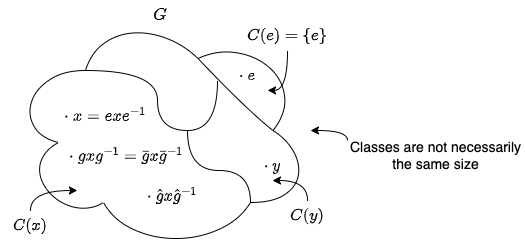
\includegraphics[width=0.95\textwidth]{Figures/Conjugacy_Partition.png}
\begin{align}
    o(G) = \sum_{\substack{\text{one elt. }\\a \text{ from} \\ \text{each conj. class}}}(\text{\# of elts in }C(a)) \nonumber
\end{align}
Recall: If $a\in G$, $N(a)=$normalizer of $a = \{g\in G | ga=ag\}$
\begin{align}
    \forall \ a \in G, N(a)<G \nonumber \\
    N(e) = G \nonumber
\end{align}
If $G$ is abelian then $N(g) = G \ \forall \ g\in G$.
\newpage
\begin{theorem}
If $G$ is a finite group, the number of elements in the class of $a$ ($C(a)$) is the index for the normalizer of that element, $N(a)$. That is,
\begin{align}
    \text{\# of elements in }C(a) \overset{\star}{=} i_G(N(a))= \frac{o(G)}{o(N(a))} \nonumber
\end{align}
Proving $\star$ will give us \textit{the class equation}:
\begin{align}
    o(G) = \sum_{\substack{\text{one  '}a'  \\\text{from each} \\ \text{conj. class}}}\frac{o(G)}{o(N(a))} \ .\nonumber
\end{align}
\textit{Proof:} The number of elements in $C(a)$ is the number of \textit{distinct} conjugates of $a\in G$. (list of $gag^-1 \ \forall \ g\in G$, toss out duplicates, then count).
\begin{align}
    i(N(a))= \text{ the number of left cosets of }N(a) \text{ in }G
\end{align}
We must show the number of distinct conjugates is the same as the number of left cosets of $N(a)$. \steezybreak\\
Plan: set up a mapping (as simply as possible), then try to show it's a bijection. \steezybreak\\
Define $\sigma:C(a)\rightarrow \{\text{left cosets of }N(a)\}$ by 
\begin{align}
    \sigma(gag^{-1})=gN(a)
\end{align}
is $\sigma$ well-defined? Take $x\in C(x)$, it's possible that $x$ might be expressed in more than one way
\begin{center}
    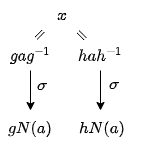
\includegraphics[width=0.19\textwidth]{Figures/sigma_well_def.png}
\end{center}%e.g. $x=gag^{-1}$ and $x=hah^{-1}$, so check that $gN(a)=hN(a)$ 
To be well-defined, $\sigma$ must send each element from the source set to one and only one element in the target set. While $\sigma$ does have somewhere to send every element (since every element in $C(a)$ can be written $gag^{-1}$ for some $g\in G$), we must ensure that when a given element $x$ can be expressed in more than one way, that it always maps to the same place, i.e. we must check that $gN(a)=hN(a)$.
\begin{align}
    gag^{-1} = hah^{-1} &\implies gag^{-1}h=ha \nonumber \\
    &\implies ag^{-1}h=g^{-1}ha \nonumber \\
    &\implies g^{-1}h \text{ commutes with } a \nonumber \\
    &\implies g^{-1}h \in N(a) \nonumber \\
    &\overset{\text{L mult. by }g}{\implies} h\in gN(a) \nonumber \\
    &\text{Now, }\underset{h\in}{gN(a)} \cap \underset{h\in}{hN(a)} \not = \emptyset \nonumber\\
    &\implies gN(a) = hN(a)
\end{align}
So $\sigma$ is well-defined. \\
\noindent \textit{$\sigma$ is surjective:} Take $yN(a) \in \text{codomain}$\\
$\sigma(yay^{-1})=yN(a)$, so $yay^{-1}$ serves as a preimage for $yN(a)$ \steezybreak\\
\noindent \textit{$\sigma$ is injective:} We want to show that this can't happen \\
\begin{center}
    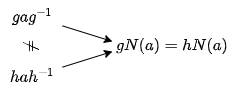
\includegraphics[width=0.4\textwidth]{Figures/noninjective.png}
\end{center}
typically to show injectivity we assume $x\not = y$ and show it follows that $\sigma(x)\not = \sigma(y)$, in this case we will prove injectivity by contraposition so we will show $\sigma(x)=\sigma(y)$ implies $x=y$, or more specifically we will assume $gN(a)=hN(a)$ and we will show this forces $gag^{-1}=hah^{-1}$
\begin{align}
    \text{Assume }gN(a)=&hN(a) \nonumber \\
    g\in hN(a) &\implies \ \exists \ n\in N(a) \ni g = hn \nonumber \\
    gag^{-1}=(hn)a(hn)^{-1}&= h\underline{na}n^{-1}h^{-1} \nonumber \\
    &= hann^{-1}h^{-1} \nonumber \\
    &=hah^{-1} \nonumber
\end{align}
 $\therefore \ \sigma$ is a bijection $\implies$ \# of elements in domain $=$ \# elements in codomain. So $o(C(a))=i_G(N(a))$. $\blacksquare$
\end{theorem}
\subsection*{Applications of the Class Equation}
\subsubsection*{Application \# 1}
\begin{theorem}
$G$ group. If $o(G)$ is a power of a prime, then the center of $G$ is bigger than just $\{e\}$.
\begin{align}
    o(G) = p^n (p \text{ prime}) \implies \text{center of }G \text{ is non-trivial} \nonumber
\end{align}
\textit{Proof:} 
\begin{align}
    a\in Z(G) &\iff ag=ga \ \forall \ g \in G \nonumber \\
    &\iff N(a)=G \nonumber \\
    &\iff i_G(N(a))=1 = \frac{o(G)}{o(N(a))}=\frac{o(G)}{o(G)} \nonumber \\
    &\underset{Thm \ 2.11.1}{\iff} \text{\# of elts. in }C(a) = 1 \nonumber \\
    &\iff C(a) = \{a\}  \ \ \ \ \ (\text{note }gag^{-1}=agg^{-1} = a \text{ since }a\in Z(G)) \nonumber
\end{align}
\begin{center}
    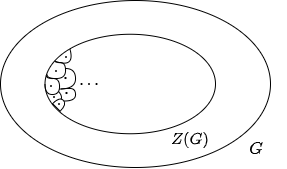
\includegraphics[width=0.45\textwidth]{Figures/shattered_center.png}
\end{center}
The partition of $G$ into equivalence classes shatters $Z(G)$ into one-point classes. Classes outside the center contain $>1$ element (notice the chain of iff statements above implies that having exactly one element in $C(a)$ is equivalent to $a\in Z(G)$).
\begin{align}
    \text{Assume } o(G)=p^n \nonumber \\
    \text{Say }o(Z(G))=\beta \ \ \ e\in Z(G) \implies \beta \geq 1 \nonumber
\end{align}
Use class equation:
\begin{align}
    o(G)= \sum_{\substack{\text{one  '}a'  \\\text{from each} \\ \text{conj. class}}} \frac{o(G)}{o(N(a))} = \beta + \sum_{\substack{\text{one $a$ } \\\text{from each }\\ \text{class outside} \\ Z(G)}} \frac{o(G)}{o(N(a))}\nonumber
\end{align}
Notice for the sum after the second equality, $N(a)<G$ but $N(a)\not = G$ because each $a$ in this sum is \textit{outside} $Z(G)$ so these $a$'s don't commute with everything. \steezybreak\\
Lagrange says $o(N(a))|o(G)=p^n$, so $o(N(a))$ is one of these: $1,p,p^2, \dots , p^{n-1}$. Say it's $p^{K_a}$, $K_a<n$ since $N(a)\not = G$, we have
\begin{align}
    p^n = \beta + \sum_{\substack{\text{one }a \\ \text{for each} \\ \text{conj. class} \\ \text{outside }Z(G)}} \frac{p^n}{p^{K_a}} = \beta + \sum p^{n-K_a}\nonumber
\end{align}
Solve for $\beta$:
\begin{align}
    \beta = p^n - \sum p^{n-K_a} \nonumber
\end{align}
Now, $p$ divides the right side so $p|\beta$. \steezybreak\\
If $\beta = 1$ then $p|1$, since no prime divides 1 $\Rightarrow\Leftarrow$, so $\beta \not = 1$. \\ So $\beta > 1$ and $G$ has non-trivial center. $\blacksquare$
\end{theorem}

\subsubsection*{Application \# 2 (Corollary to Thm 2.11.2)}
In the proof below we use a new symbol $A\subsetneqq B$ to indicate that $A$ is a strict subset of $B$, this symbol is equivalent to $A \subset B$ \textit{and} $B \not \subset A$
\begin{corollary}
A group of order $p^2$ ($p$ prime) is abelian. \steezybreak\\
\noindent \textit{Proof:} Suppose $o(G)=p^2$, we will show $Z(G)=G$.\steezybreak\\
Now, $Z(G)<G \ \ \implies o(Z(G)) = 1, \ p, \ \text{ or} \underbrace{p^2}_{\text{we want this}}$. \steezybreak\\
By Thm 2.11.2, $Z(G)$ is bigger than $\{e\}$ so order of $Z(G)$ is not $1$. What if $o(Z(G))= p$?
\begin{center}
    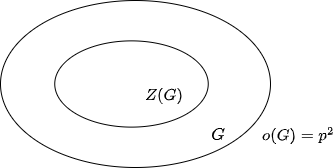
\includegraphics[width=0.5\textwidth]{Figures/Center_of_G.png}
\end{center}
Then $\exists \ a \in G \ni \ a \not\in Z(G)$ \steezybreak\\
Consider $N(a)$: 
\begin{align}
    \underset{a\not \in }{Z(G)} \subsetneqq &\underset{a\in}{N(a)}, \text{ so order of }N(a)>p \nonumber \\ 
    \text{Now, since }N(a) < G, \ \ o(N(a))>p &\implies o(N(a))=p^2 \nonumber \\
    &\implies N(a) = G \nonumber \\
    &\implies a \text{ commutes with everything!} \Rightarrow\Leftarrow
\end{align}
($\Rightarrow\Leftarrow$ because $a\not\in Z(G)$) \steezybreak\\
This contradiction gives that $o(Z(G))\not = p$ \steezybreak\\
So $o(Z(G))$ must be $p^2$, thus $Z(G)=G$ \steezybreak\\
$\therefore$ $G$ is abelian. $\blacksquare$
\end{corollary}

How much information do you get about a group from its order?
\subsection*{Fact Collection w.r.t. $o(G)=p, \ p^2, \ p^n, ...$ ($p$ prime): }
\subsubsection*{$o(G)=p$}
\begin{center}
    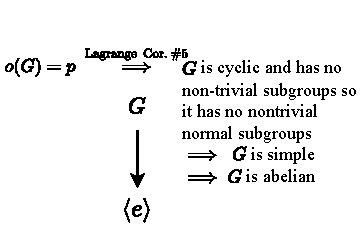
\includegraphics[width=0.495\textwidth]{Figures/prime_order_lattice.pdf}
    \begin{align}
        \Z_7 = \{0,1,2,3,4,5,6\} \text{ under } \ +\mod 7\nonumber
    \end{align}
\end{center}
\subsubsection*{$o(G)=p^2$}
\begin{align}
        o(G)=p^2 \ \implies G \text{ abelian} \ \implies \text{All subgroups of }G \text{ are normal in }G. \nonumber 
\end{align}
\begin{center}
    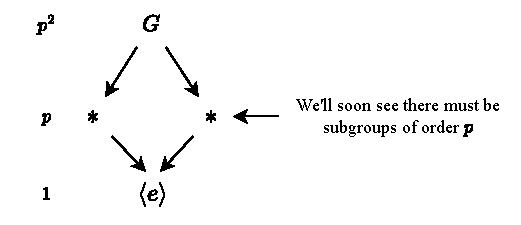
\includegraphics[width=0.7\textwidth]{Figures/prime_squared_order_lattice.pdf}
\end{center}
\subsubsection*{$o(G)=p^n$}
\begin{center}
    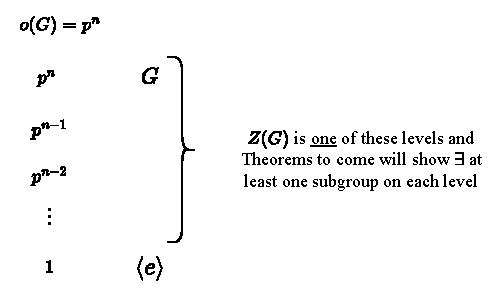
\includegraphics[width=0.68\textwidth]{Figures/prime_power_order_lattice.pdf}
\end{center}
\begin{tcolorbox}
    \begin{center}
        $\star\star\star$ \textbf{Read up to this point to Complete Homework 7 (Located in \ref{sec:HW7})} $\star\star\star$
    \end{center}
\end{tcolorbox}

\section{\texorpdfstring{The Sylow Theorems ( $G$ finite )}{The Sylow Theorems ( G finite )}}
Lagrange's theorem tells us that the order of a subgroup of a finite group is a divisor of the order of that group. The converse, however, is false. There are very few theorems which assert the existence of subgroups of prescribed order in arbitrary finite groups. The most basic, and widely used, is a classic theorem due to the Norwegian mathematician Peter Sylow (1832-1918).
In this section we will present this classic result. \\

\noindent Before beginning the proof of Sylow's first theorem, we will take a slight detour to a number-theoretic and combinatorial argument that will be useful in our proof: \\
The number of ways of picking a subset of $k$ elements from a set of $n$ elements can easily be shown to be 
\begin{equation}
    {n \choose k} = {\frac{n!}{k!(n-k)!}} \nonumber
\end{equation}

If $n=p^\alpha m$ where $p$ is a prime number, and if $p^r|m$ but $p^{r+1}\not | \ m$, consider
\begin{align}
    {p^\alpha m \choose p^\alpha} &= \frac{(p^\alpha m)!}{(p^\alpha)!(p^\alpha m - p^\alpha)!} \nonumber \\
    &= \frac{p^\alpha m (p^\alpha m -1)(p^\alpha m - 2)\dots(p^\alpha m - p^\alpha + 1)\overbrace{(p^\alpha m - p^\alpha)(p^\alpha m -p^\alpha -1)\dots(p^\alpha m - p^\alpha m + 1)}^{(p^\alpha m -p^\alpha)!}}{(p^\alpha)!(p^\alpha m -p^\alpha)!} \nonumber \\
    &= \frac{p^\alpha m (p^\alpha m -1)(p^\alpha m - 2)\dots(p^\alpha m - p^\alpha + 1)}{(p^\alpha)!} \nonumber \\
    &= \frac{p^\alpha m (p^\alpha m -1) \dots (p^\alpha m - i) \dots (p^\alpha m - p^\alpha +1)}{p^\alpha (p^\alpha -1) \dots (p^\alpha - i) \dots (p^\alpha - p^\alpha +1)} \nonumber \\
    &= m\cdot \frac{p^\alpha (p^\alpha m -1) \dots (p^\alpha m - i) \dots (p^\alpha m - p^\alpha +1)}{p^\alpha (p^\alpha -1) \dots (p^\alpha - i) \dots (p^\alpha - p^\alpha +1)} \nonumber \\ 
    &= m\cdot \frac{ (p^\alpha m -1) \dots (p^\alpha m - i) \dots (p^\alpha m - p^\alpha +1)}{ (p^\alpha -1) \dots (p^\alpha - i) \dots (p^\alpha - p^\alpha +1)}
\end{align}
The question is, What power of $p$ divides ${p^\alpha m \choose p^\alpha}$? We will show that $p^r | {p^\alpha m \choose p^\alpha}$ but $p^{r+1} \not | {p^\alpha m \choose p^\alpha}$. \\
\textit{Proof:} Let $m\geq 1$, and $0<i<p^\alpha$, with $m,i,p,\alpha,\beta \in \Z$. \steezybreak\\ In order to prove our claim, we will begin by showing that the fraction on the right of equation (2.7) cannot provide any factors of $p$ since each numerator term that could provide a factor of $p$ will cancel with a corresponding term in the numerator. That is, we will begin by proving the following claim. \steezybreak\\
\textit{Claim 1: } $p^\beta | p^\alpha m - i \ \iff p^\beta | p^\alpha - i$  for $0<i<p^\alpha$\steezybreak\\
\textit{Proof of Claim 1:}\steezybreak\\
\textbf{$\Leftarrow$ :} Suppose $p^\beta | p^\alpha -i $
\begin{align}
  &\implies \exists \ h \in \Z \ni hp^\beta = p^\alpha - i \ \ \ \ \ (\text{Note, }i<p^\alpha \implies h > 0)\nonumber \\
  &\implies i = p^\alpha - hp^\beta \nonumber \\
  &\implies p^\alpha m -i = p^\alpha m - p^\alpha + hp^\beta \nonumber \\
  &\implies p^\alpha m -i = p^\beta (p^{\alpha-\beta}m-p^{\alpha-\beta}+h) \nonumber
\end{align}
\indent \textit{claim: } $\beta < \alpha$, otherwise $i=p^\alpha - \underbrace{h}_{>0}p^\beta \leq 0, \text{ but } i>0 \Rightarrow \Leftarrow \ \text{So } \beta < \alpha$
\begin{align}
    &\implies p^{\alpha -\beta} \in \Z \nonumber \\
    &\implies (p^{\alpha-\beta}m-p^{\alpha-\beta}+h) \in \Z \nonumber \\
    &\implies p^\beta | p^\alpha m -i \nonumber
\end{align}

\textbf{$\Rightarrow$:} Suppose $p^\beta | p^\alpha m -i$
\begin{align}
    &\implies \exists \ g \in \Z \ni gp^\beta = p^\alpha m -i \nonumber \\
    &\implies i = p^\alpha m -gp^\beta \nonumber \\
    &\implies p^\alpha - i = p^\alpha - p^\alpha m + gp^\beta \nonumber \\
    & \ \ \ \ \ \ \ \ \ \ \ \ \ \ \ \ \ \ \ \ = p^\beta (p^{\alpha-\beta} -p^{\alpha-\beta}m + g) \nonumber
\end{align}
\indent \textit{claim: } $\beta < \alpha$, otherwise 
\begin{align}
    i &= p^\alpha m - gp^\beta \nonumber \\
    \implies p^\alpha -i &= p^\alpha - p^\alpha m + gp^\beta \nonumber \\
    &= p^\alpha \underbrace{((1-m)+gp^{\overbrace{\scriptstyle\beta-\alpha}^{>0}})}_{\in \Z} \nonumber \\
    &\implies p^\alpha | p^\alpha - i \ \ \Rightarrow\Leftarrow \nonumber 
\end{align}
So $\beta < \alpha \ \ \implies (p^{\alpha-\beta}-p^{\alpha-\beta}m+g)\in \Z$ $ \ \ \ \implies \ \ p^\beta | p^\alpha - i$. This completes the proof of claim 1. \steezybreak\\
With Claim 1 established we can now see that if there were some numerator term $p^\alpha m - i$ for $0<i<p^\alpha$ that has a power of $p$ as a factor then there is \textit{necessarily} a corresponding term in the denominator ($p^\alpha -i$) which cancels this power of $p$. This means if any power of $p$ divides ${p^\alpha m \choose p^\alpha}$ it must do so by dividing the $m$ out front in equation (2.7). Thus
\begin{align}
    p^r | {p^\alpha m \choose p^\alpha} \text{ but } p^{r+1} \not | {p^\alpha m \choose p^\alpha} \ \ \ \ \ \ \blacksquare \nonumber 
\end{align}
%Looking at this number how we have it written out in the last line, we can see that except for the term $m$ in the numerator, the power of $p$ dividing $(p^\alpha m -i)$ is the same as that dividing $p^\alpha$

\begin{theorem}[Sylow's Theorem (Sylow \#1)]
$G$ finite. If $p$ is prime and $p^\alpha|o(G)$ then $G$ has a subgroup of order $p^\alpha$ \steezybreak\\
\textit{Proof:}
Let $\mathcal{M}$ be the set of all subsets of $G$ which have $p^\alpha$ elements. Since $p^\alpha | o(G)$, $o(G)$ can be written $o(G)=p^\alpha m$ for some $m\in \Z \ni m \geq 1$. Thus $\mathcal{M}$ has ${p^\alpha m \choose p^\alpha}$ elements. Given $M_1 , M_2 \in \mathcal{M}$ ($M_1$ is a subset of $G$ having $p^\alpha$ elements, and likewise so is $M_2$ ) define $M_1 \sim M_2$ if there exists an element $g \in G$ such that $M_1 = M_2g$. It is immediate to verify that this defines an equivalence relation on $\mathcal{M}$.
\begin{enumerate}[label=\roman*)]
    \item Reflexivity: $M_1=M_1e$, $e\in G$
    \item Symmetry: Let $M_1\sim M_2 $
    \begin{align}
        &\implies \exists \ g\in G \ni M_1=M_2g, \nonumber \\
        &\implies M_1g^{-1} = M_2gg^{-1}=M_2 \nonumber \\
        G \text{ group } &\implies \ g^{-1}\in G \nonumber \\
        &\implies M_2\sim M_1 \nonumber 
    \end{align}
    \item Transitivity: Let $M_1\sim M_2$ and $M_2\sim M_3$
    \begin{align}
        M_1\sim M_2 &\implies \exists \ g \in G \ni M_1= M_2g \nonumber \\
        M_2\sim M_3 &\implies \exists \ h \in G \ni M_2= M_3h \nonumber \\
        &\implies M_1 = (M_3h)g = M_3(hg) \ \  hg\in G \text{ by closure.} \nonumber
    \end{align}
\end{enumerate}


We claim that there is at least one equivalence class of elements in $\mathcal{M}$ such that the number of elements in this class is not a multiple of $p^{r+1}$, for if $p^{r+1}$ is a divisor of the size of each equivalence class, then $p^{r+1}$ would be a divisor of the number of elements in $\mathcal{M}$ (remember observation 4 about division and that an equivalence relation on a set partitions the set). Since $\mathcal{M}$ has ${p^\alpha m \choose p^\alpha}$ elements and $p^{r+1} \not | {p^\alpha m \choose p^\alpha}$ this cannot be the case. Let ${M_1, \dots , M_n}$ be such an equivalence class in $\mathcal{M}$ where $p^{r+1}\not | \ n $. By our very definition of equivalence in $\mathcal{M}$, if $g \in G$, for each $i = 1, \dots , n$, $M_ig = M_j$ for some $j, 1 \leq j \leq n$. We let $H = \{g \in G | M_1g = M_1 \}$. Clearly $H$ is a subgroup of $G$ by Lemma 2.4.2, for if $a, b \in H$, then $M_1a = M_1 $ and $ M_1 b = M_1$ therefore $M_1ab = (M_1a)b = M_1b =M_1$. We would like to show $o(H)=p^\alpha$. We first claim that $n\cdot o(H) =o(G)$. \steezybreak\\
\textit{Proof of Claim:}
We will prove that $no(H)=o(G)$ by first showing that there is a bijection from $\{Ha | a \in G\}$ to $\{M_1,\dots M_n\}$. \steezybreak\\
Let $C= \{Ha|a\in G\}$ be the set of right cosets of $H$. Then,
\begin{align}
    |C| = \frac{o(G)}{o(H)} 
\end{align}
Note that
\begin{align}
    Ha=Hb \iff ab^{-1} \in H \iff M_1 ab^{-1} = M_1 \iff M_1a=M_1b .\nonumber
\end{align}
Therefore the function $\sigma:C\rightarrow \mathcal{M}$ given by $\sigma(Ha)=M_1 a$ is well-defined and injective. Since $M_1aa^{-1}=M_1$, we have $M_1a\sim M_1$ and thus $\sigma(C) \subset \{M_1,M_2,\dots M_n\}$. On the other hand, each $M_i$ has the form $M_1a_i$ because $M_i \sim M_1$. So, $M_i = \sigma(Ha_i)$ and thus $\{M_1, \dots, M_n\} \subset \sigma(C)$. This shows that $\sigma(C)= \{M_1, \dots , M_n\}$. So $\sigma$ is a one-to-one correspondence (a bijection), we conclude that
\begin{align}
    |C|=|\{M_1,\dots M_n\}|
\end{align}
Equations (2.8) and (2.9) imply $|C|o(H)=n\cdot o(H)=o(G)$. This completes the proof of the claim.

Now $no(H) = o(G) = p^\alpha m$; since $p^{r+1}\not | n$ and $p^{r+\alpha}|p^{\alpha}m = no(H)$, it must follow that $p^\alpha | o(H)$, and so $o(H)\geq p^\alpha$. However, if $m_1 \in M_1$ , then for all $h\in H, m_1h \in M_1$. Thus $M_1$ has at least $o(H)$ distinct elements. However, $M_1$ was a subset of $G$ containing $p^\alpha$ elements. Thus $p^\alpha \geq o(H)$. Combined with $o(H) \geq p^\alpha$ we have that $o(H) = p^\alpha$. \textit{But then we have exhibited a subgroup of $G$ having exactly $p^\alpha$ elements, namely $H$.} This proves the theorem; it actually has done more -- it has constructed the required subgroup before our very eyes! $\blacksquare$

\end{theorem}

\begin{example}
Consider $A_4$ whose order is $o(A_4)= \frac{4!}{2} = 12 =2^2\cdot 3$ \\ 
\noindent Sylow \#1 $\implies$ $A_4$ has subgroups of order $2,2^2$ and $3$ \steezybreak\\
\noindent Sylow \#1 tells us nothing about $6$ because $6$ is not a prime power.
\end{example}

\begin{definition}[p-Sylow Subgroup]
If $H<G$ and $o(H)=p^m$ where $p^m|o(G)$ but $p^{m+1}\not | o(G)$, the $H$ is a \textit{p-Sylow subgroup} of $G$.
\end{definition}

\begin{example}
Given $G$ with $o(G)=72=8\cdot 9=2^3\cdot 3^2$, Sylow \#1 says $G$ has subgroups of order $2,2^2,2^3,3,3^2$. The order $8$ subgroups are $2-$Sylow subgroups and the order $9$ subgroups are $3-$Sylow subgroups.
\end{example}
\begin{example}
Let $o(G)=8=2^3$, the $2-$Sylow subgroup is the trivial group $G$.
\end{example}

To save on time the next two theorems will be provided without proof as we are currently more interested in the insights that can be gained from the results themselves. (Jack, get some proofs for these!)

\begin{theorem}[Sylow \#2] 
For a given prime $p$, the $p-$Sylow subgroups are conjugate to each other.
\end{theorem}
Sylow \#2 says that if you know one $p-$Sylow subgroup $H$, you can find the rest of the $p-$Sylow subgroups by conjugating $H$.\\
\begin{center}
    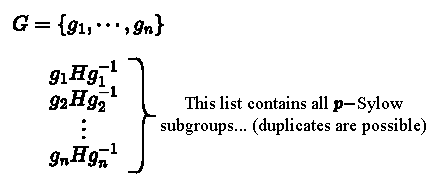
\includegraphics[width=0.5\textwidth]{Figures/Sylow2_conjugates.pdf} 
\end{center}
\begin{theorem}[Sylow \#3]
Suppose $p^m|o(G)$ but $p^{m+1}\not | o(G)$. The number of $p-$Sylow subgroups in $G$:
\begin{enumerate}
    \item divides $\frac{o(G)}{p^m}$ (the index of the $p-$Sylow subgroup) \steezybreak\\
    \noindent AND
    \item is congruent to $1\mod p$ \ \ \ (i.e. is $1+kp$ for some $k\in \Z$)
\end{enumerate}
\end{theorem}
\begin{example}
Let $o(G)=12=2^2\cdot 3$ \steezybreak\\
Sylow \#1 guarantees that $G$ has $2-$Sylow subgroup(s) of order $4$, $3-$Sylow subgroup(s) of order 3, and at least one subgroup of order $2$. \steezybreak\\
How many $2-$Sylow subgroups are there? \steezybreak\\
Sylow \#3 says the number of $2-$Sylow subgroups must divide the index of $2-$Sylow (12/4 = 3) and must be congruent to 1 mod 2 so there are either 1 or 3 $2-$Sylow subgroups. \steezybreak\\
($A_4$ has one subgroup of order 4; $D_6$ has 3 subgroups of order 4) \steezybreak\\
How many $3-$Sylow subgroups? Well the first part of Sylow \#3 tells us the number of $3-$Sylow subgroups divide $\frac{12}{3}=4$ making 1, 2, and 4 candidates, the second part of Sylow \#3 says the number must be $\equiv 1\mod 3$ which eliminates $2$ as a candidate, so there must be 1 or 4 $3-$Sylow subgroups. \steezybreak\\
($A_4$ has 4 ; $D_6$ has 1)
\newpage
\end{example}

\subsection*{Applications of Sylow Theorems}
\begin{enumerate}
    \item Prove no group of order $50$ is simple. \steezybreak\\
    \includegraphics[width=0.575\textwidth]{Figures/order50_no_normal.pdf} \steezybreak\\
    \textit{Proof:} $G$ group with order $o(G)=50=2\cdot 5^2$, $G$ has subgroups of order $2, 5, 25$. Consider one of the subgroups of order $25$, call it $H$
    \begin{align}
        &i_G(H)=2 \ \ \overset{Cor \ 2.6.2}{\Longrightarrow} \ \  H\triangleleft G \nonumber \\
        &\therefore G \text{ is not simple.} \ \ \blacksquare \nonumber
    \end{align}
    \item Any two groups of order $15$ are isomorphic. \steezybreak\\
    \textit{Proof: } Suppose $G$ is a group and $o(G)=15=3\cdot 5$\\
    Sylow \#1 $\implies$ $\exists$ in $G$ at least one subgroup of order $3$ and one of order $5$.\\
    Sylow \#3 $\implies$ \# of $5-$Sylow subgroups must divide $\frac{15}{5}=3$ (so $1$ or $3$) AND must be $\equiv 1\mod 5$ $\implies$ there is exactly 1 subgroup of order $5$, call it $H$\\
    Sylow \#3 $\implies$ \# of $3-$Sylow subgroups must divide $\frac{15}{3}=5$ (so $1$ or $5$) AND must be $\equiv 1\mod 3$ $\implies$ $G$ has exactly one subgroup of order $3$, call it $K$.\\
    \includegraphics[width=0.5\textwidth]{Figures/order15_subgroups.pdf}\\
    \begin{align}
        &H\cap K < H \text{ and } H\cap K < K \nonumber \\
        &\text{Take }x\in G, x\not\in H\cup K \nonumber \\
        &\text{Order of }x \text{ can be }1, 3, 5,\text{ or }15 \nonumber\\
        &x\text{ is not } e \text{ so order }\neq 1 \nonumber \\
        &\text{If }o(x)=3, \text{ then } \langle x \rangle = K \nonumber \\
        &\Rightarrow\Leftarrow x \not \in K \nonumber \\
        &\text{If }o(x)=5, \text{ then } \langle x\rangle = H \nonumber \\
        &\Rightarrow\Leftarrow x\not \in H \nonumber
    \end{align}
    So the order of $x$ must be $15$. \steezybreak\\
    So $\langle x \rangle = G$. \steezybreak\\
    $\therefore \ \ G$ is cyclic. \\
    So any group of order $15$ is cyclic. If $o(G)=o(\bar{G})=15$ then $G$ and $\bar{G}$ are isomorphic because any 2 cyclic groups of the same order are isomorphic (important fact right before the 1st Isomorphism Theorem). $\ \ \ \ \blacksquare$
    \item Any group of order 20,449 is abelian. \steezybreak\\
    \noindent \textit{Proof:} Let $o(G)=20,449=11^2\cdot 13^2$ \steezybreak\\
    Sylow \#3 $\implies$ \# of 11-Sylow subgroup(s) divides $\frac{o(G)}{11^2}=13^2$ : \# is $1$, $13$, or $13^2$. Also, \# $\equiv 1 \mod 11$, remove 13 because $13\equiv 2\mod 11$ and $13^2\equiv 4\mod 11$. So $G$ has exactly $1$ 11-Sylow subgroup, call it $H$. \steezybreak\\
    \begin{align}
        o(H)&=11^2=121 \nonumber \\
        H &\text{ is abelian (order }p^2) \nonumber \\
        H&\triangleleft G \text{(unique of its order)} \nonumber
    \end{align}
    Now, the \# of 13-Sylow subgroups must divide $\frac{o(G)}{169}=11^2$, so $1, 11, 121$ are candidates. The \# also must be $\equiv 1 \mod 13$, $11\equiv 11\mod 13$, $121 \equiv 4 \mod 13$, so there is exactly one $13$-Sylow subgroup, call it $K$.
    \begin{align}
        o(K)&=13^2=169\nonumber \\
        K &\text{ is abelian }(o(K)=p^2) \nonumber \\
        K&\triangleleft G  \text{(unique of it's order)} \nonumber
    \end{align}
    Now recall from Theorem 2.5.1
    \begin{align}
        o(HK)= \frac{o(H)o(K)}{o(H\cap K)} \nonumber \\
        o(H\cap K) | o(H)=11^2 \implies o(H\cap K) = 1, 11, 121 \nonumber \\
        o(H\cap K) | o(K)=13^2 \implies o(H\cap K) = 1, 13, 169 \nonumber \\
        \implies  o(H\cap K) = 1 \nonumber \\
        \implies o(HK) = \frac{o(H)o(K)}{o(H\cap K)}= \frac{11^2\cdot 13^2}{1} = o(G) \nonumber \\
        \implies HK = G \nonumber
    \end{align}
    So do elements of $H$ commute with elements of $K$? Take $h\in H$ and $k\in K$ and consider commutator $[h,k]$
    \begin{align}
        [h,k] &= hkh^{-1}k^{-1} = \underbrace{(\underset{\in G}{h}\underset{\in G}{k}h^{-1})}_{\in K}k^{-1} \in K  \ \ \  (\text{by } K\triangleleft G \text{ and } K \text{ group (closure)}.) \nonumber \\
        [h,k] &= h\underbrace{(kh^{-1}k^{-1})}_{\in H} \in H \nonumber \\
        &hkh^{-1}k^{-1} \in H\cap K \leftarrow \text{ one element, }e \nonumber \\
        e&= hkh^{-1}k^{-1} \nonumber \\
        &\implies kh=hk \nonumber \\
        &\therefore \text{ elements in }H \text{ commute with elements in }K. \nonumber
    \end{align}
    Take $x,y \in G$, then since $G=HK$ we have $x=hk$ and $y=\bar{h}\bar{k}$ for some $h,\bar{h}\in H$ and $k,\bar{k}\in K$.
    \begin{align}
        xy&=hk\bar{h}\bar{k}=h\bar{h}k\bar{k}=\bar{h}h\bar{k}k=\bar{h}\bar{k}hk=yx \nonumber \\
        &\therefore \ G \text{ abelian}. \ \ \ \ \ \ \blacksquare \nonumber
    \end{align}
\end{enumerate}
% Artificially setting back section and theorem counters so this thm number reflects what is in Herstein's Topics in Alg. 2 Ed.
\setcounter{dummy}{2}
\setcounter{section}{11}
\begin{theorem}[Cauchy's Theorem]
If $p$ is prime and $p|o(G)$ then $G$ has an element of order $p$. \steezybreak\\
\noindent \textit{Proof:} $p|o(G) \ \implies \ G$ has a subgroup $H$ of order $p$ (Sylow \#1). 
\begin{align}
    o(H) \text{ prime }&\implies H \text{ is cyclic }\nonumber \\
    &\implies H=\langle x \rangle, \text{ and }o(x) = p. \ \ \ \blacksquare \nonumber
\end{align}
\end{theorem}
\setcounter{dummy}{2}
\setcounter{section}{12}


\begin{enumerate}
\setcounter{enumi}{3}
    \item Prove: No group of order $125$ is simple. \steezybreak\\ 
    $o(G)=125=5^3$, The $5$-Sylow subgroup has order $125$ -- it is $G$.
    \begin{align}
        o(G)=p^n \implies Z(G)\neq \{e\} \nonumber
    \end{align}
    So if $Z(G)\neq \{e\}$ then $Z(G)$ is the non-trivial normal subgroup we seek. \\
    If $Z(G)=G \ \ \implies \ \ G$ is abelian and every subgroup is normal. \\
    Cauchy $\implies \ \exists \ a\in G \ni \ o(a)=5$ \\
    Then $H=\langle a \rangle = \{a,a^2,a^3,a^4,e\}$ and $H\triangleleft G$ \\
    $\therefore \ G$ is not simple, it always has a non-trivial normal subgroup.
\end{enumerate}
This weeks homework (HW \#8) largely deals with Sylow theorems.

\section{Direct Products}

\begin{definition}[Direct Products of Groups]
Let $G$ and $\bar{G}$ be groups of orders $m$ and $n$ respectively. The (external) \textit{direct product} of $G$ and $\bar{G}$ is defined as follows:
\begin{align}
    G\times \bar{G} = \{(\ g,\bar{g}) \  | \ g\in G, \bar{g}\in \bar{G}\} \nonumber
\end{align}
\end{definition}

\begin{proposition}
    $G\times \bar{G}$ is a group of order $nm$ under \textit{component-wise product}.\steezybreak\\
    \begin{align}
        (g,\bar{g})\circ (h,\bar{h}) = (g \underset{\cdot \text{ in } G}{\cdot} h \ \ , \ \  \bar{g}\underset{\cdot \text{ in }\bar{G}}{\cdot}\bar{h}) \nonumber
    \end{align}
    \textit{Proof:} Take $(g,\bar{g}), (h,\bar{h}), (k,\bar{k})\in G\times \bar{G}$
    \begin{enumerate}
        \item Closure: $(g,\bar{g})(h,\bar{h})= (\underset{\in G \text{ by closure of } G}{g \ \cdot \ h},\underset{\in \bar{G} \text{ by closure of } \bar{G}}{\bar{g}\ \cdot \ \bar{h}}) \in G\times \bar{G}$ \\ $\therefore$ $G\times \bar{G}$ is closed under component-wise products.
        \item Associativity: 
        \begin{align}
            [(g,\bar{g})(h,\bar{h})](k,\bar{k}) & \nonumber \\
            &= (gh,\bar{g}\bar{h})(k,\bar{k}) \nonumber \\
            &= ((gh)k,(\bar{g}\bar{h})\bar{k}) \nonumber \\
            &= (g(hk),\bar{g}(\bar{h}\bar{k})) \ \ \ \ \ (G \text{ and } \bar{G} \text{ associative.}) \nonumber \\
            &= (g,\bar{g})[(h,\bar{h})(k,\bar{k})]\nonumber
        \end{align}
        \item Identity: $(e,\bar{e}) \in G\times \bar{G}$ serves as identity:
        \begin{align}
            (e,\bar{e})(g,\bar{g})=(eg,\bar{e}\bar{g})= (g,\bar{g}) \nonumber \\
            (g,\bar{g})(e,\bar{e})=(ge,\bar{g}\bar{e})=(g,\bar{g}) \nonumber
        \end{align}
        \item Inverses: Take $(g,\bar{g})\in G\times \bar{G}$
        \begin{align}
            (g^{-1},\bar{g}^{-1})(g,\bar{g}) &= (g^{-1}g,\bar{g}^{-1}\bar{g})=(e,\bar{e})=e\in G\times \bar{G} \nonumber \\
            (g,\bar{g})(g^{-1},\bar{g}^{-1}) &= (gg^{-1},\bar{g}\bar{g}^{-1})=(e,\bar{e}) = e \in G\times \bar{G} \nonumber \\
            &\therefore (g^{-1},\bar{g}^{-1})\in G\times \bar{G} \nonumber
        \end{align}
        and by uniqueness of inverses $(g^{-1},\bar{g}^{-1})$ \textul{is} $(g,\bar{g})^{-1}$. \\
    \end{enumerate}
    $o(G\times \bar{G})$ is the number of possible pairs $(g,\bar{g})$ with $g\in G$ ($o(G)=n$ choices), $\bar{g}\in \bar{G}$ ($o(\bar{G})=m$ choices).
    \noindent $\therefore \ $ number of pairs $=o(G)\cdot o(\bar{G})=n\cdot m$. $\blacksquare$ \steezybreak\\
    \noindent Also note that if $G$ and $\bar{G}$ are abelian, $G\times \bar{G}$ is abelian:
        \begin{align}
            (x,\bar{x})(y,\bar{y})=(xy,\bar{x}\bar{y}) = (yx,\bar{y}\bar{x})=(y,\bar{y})(x,\bar{x}). \nonumber
        \end{align}
\end{proposition}

\begin{example}[HW\#5 Problem 4]
    Let $G=\bar{G}=\R$ under $+$ \\ 
    $G\times \bar{G}= \R^2$ under vector addition (component-wise) \\
    \begin{align}
        (r,s)(r',s')=(r+r',s+s') \nonumber \\
        \text{identity }= (0,0) \nonumber \\
        (r,s)^{-1}= (-r,-s) \nonumber
    \end{align}
\end{example}
\begin{example}
    Let $G=\bar{G}=\R-\{0\}$ under multiplication \\
    $G\times \bar{G}$ is $R^2$ with axes removed. \\
    \begin{align}
        (r,s)(r',s')=(rr',ss') \nonumber \\
        (r,s)^{-1} = (1/r,1/s) \nonumber \\
        \text{identity }= (1,1). \nonumber
    \end{align}
\end{example}
\noindent Both of the previous two examples are infinite groups.
\begin{example}
\begin{align}
    &\Z_2\times \Z_3 \nonumber \\
    &\Z_2 = \{0,1\} \text{ under }+\mod 2 \nonumber \\
    &\Z_3 = \{0,1,2\} \text{ under }+\mod 3 \nonumber \\
    &o(\Z_2\times \Z_3)= 2\cdot 3 = 6  \ \  (\leftarrow \text{possible orders of elts are } 1, 2, 3, 6)\nonumber 
\end{align}
Let's have a look at the order of the elements in $\Z_2\times \Z_3$:
\begin{table}[h!]
    \centering
    \begin{tabular}{c|c}
         elts in $\Z_2\times \Z_3$& order   \\ \hline
         (0,0) & 1 \\
         (0,1) & 3 \\
         (0,2) & 3 \\
         (1,0) & 2 \\
         (1,1) & 6 \\
         (1,2) & 6 
    \end{tabular}
    \label{tab:elts_Z2_cross_Z3}
\end{table}
\end{example}

\begin{example}
    $\Z_3\times \Z_3$ order $=9=3\cdot 3$, potential element orders are $1, 3, 9$
    \begin{table}[ht!]
    \centering
    \begin{tabular}{c|c}
         elts in $\Z_3\times \Z_3$& order   \\ \hline
         (0,0) & 1 \\
         (0,1) & 3 \\
         (0,2) & 3 \\
         (1,0) & 3 \\
         (1,1) & 3 \\
         (1,2) & 3 \\
         (2,0) & 3 \\
         (2,1) & 3 \\
         (2,2) & 3 
    \end{tabular}
    \label{tab:elts_Z3_cross_Z3}
\end{table}
Interestingly, unlike in the previous example, there is no element here with order equal to the order of the group! Even though $\Z_3$ is cyclic on its own, $\Z_3\times \Z_3$ has no generator and is not cyclic. In fact, there is a necessary and sufficient condition for a direct product of cyclic groups to be cyclic, which we will introduce next.
\end{example}
\newpage
\begin{proposition}
    If $G$ and $\bar{G}$ are cyclic, then $G\times \bar{G}$ is cyclic $\iff$ order of $G$ and order of $\bar{G}$ are relatively prime. \steezybreak\\
    \textit{Proof}: We want to prove the following for cyclic groups $G$ and $\bar{G}$: 
    \begin{align}
        G\times\bar{G} \text{ cyclic } \iff GCD(o(G),o(\bar{G}))=1 \nonumber
    \end{align}
We will begin by showing RHS $\implies$ LHS. \steezybreak\\
\noindent \textbf{$\Leftarrow$ :} \steezybreak\\
\noindent Suppose $G$ and $\bar{G}$ are cyclic groups with $o(G)=n$, $o(\bar{G})=m$ and $GCD(m,n)=1$. We must show that $G\times \bar{G}$ has an element of order $nm$ (i.e. a generator)
\begin{align}
    G \text{ cyclic }\implies \exists \ a \in G \ni G= \langle a \rangle \nonumber \\
    \bar{G} \text{ cyclic }\implies \exists \ \bar{a} \in \bar{G} \ni \bar{G}= \langle \bar{a} \rangle \nonumber 
\end{align}
What is the order of $(a,\bar{a})$ (we hope it's $nm$)
\begin{align}
    (a,\bar{a})^{nm} \underset{\text{componentwise}}{=} (a^{nm},\bar{a}^{nm}) =((a^n)^m,(\bar{a}^m)^n) = ((e)^m,(\bar{e})^n)=(e,\bar{e}). \nonumber
\end{align}
By the result from problem \#1 of HW\#4 $\implies$ $o((a,\bar{a}))|nm$, call $o((a,\bar{a}))=s$. \steezybreak\\
\begin{center}
\boxed{s \ | \ nm} 
\end{center}
On the other hand
\begin{align}
    (e,\bar{e})=(a,\bar{a})^s = (a^s,\bar{a}^s) \nonumber \\
    a^s= e \implies o(a)|s \implies n | s \implies \exists \ x \in \Z \ni s=xn \nonumber \\
    \bar{a}^s = \bar{e} \implies o(\bar{a})|s \implies m|s \implies m | xn \nonumber
\end{align}
By Lemma 1.3.2, since $m|xn$ and $GCD(m,n)=1$ $\implies$ $m|x$
\begin{align}
    m|x \implies \exists \ t\in \Z \ni x=tm \nonumber \\
\text{But then, } s=xn=tmn = \underset{\in \Z}{t}(mn) \nonumber \\
    \therefore mn|s \nonumber
\end{align}
Then, by observation \#2 from Section 1.3 $\implies \ \ s=\pm mn \ \implies s=mn$
\begin{align}
    &\therefore (a,\bar{a}) \text{ generates } G\times \bar{G} \nonumber \\
    &\therefore G\times \bar{G} \text{ is cyclic.} \nonumber
\end{align}
\noindent \textbf{$\Rightarrow$ :} \steezybreak\\
\noindent Assume $G\times \bar{G}$ cyclic with $o(G)=n$, $o(\bar{G})=m$ and suppose $GCD(n,m)=d$.

\begin{align}
&d | n \implies \exists x\in \Z \ni n=xd \nonumber \\
&d | m \implies \exists y\in \Z \ni m=yd \nonumber
\end{align}
$G\times \bar{G}$ cyclic $\implies \ \exists $ an elt. $(g,\bar{g})\in G\times \bar{G}$ with order $nm=xdyd$. \steezybreak\\
But $(g,\bar{g})^{xyd} = (g^{xyd},\bar{g}^{xyd})=((g^{xd})^y, (\bar{g}^{yd})^x)$ \steezybreak\\
Lagrange Corr. \#2 $\implies$ $(e^y,\bar{e}^x)=(e,\bar{e})$, thus $xyd \geq xdyd \implies 1\geq d$ but $d$ is a positive integer $\therefore$ $d$ must $=1$.\steezybreak\\
$\therefore GCD(n,m)=1$. $\blacksquare$
\end{proposition}

All of these ideas may be extended to $K$ groups ($K>2$). \steezybreak\\
$G_1\times G_2 \times \dots \times G_K$ is a group under component-wise product, $o(G_1\times G_2\times \dots \times G_K)=o(G_1)\cdot o(G_2) \dots \cdot o(G_K)$. If $G_1$, $G_2$, ..., $G_K$ are cyclic, then $G_1\times G_2\times \dots \times G_K$ is cyclic $\iff$ $GCD(o(G_i),o(G_j))=1 \ \forall \text{ pairs } 1\leq i,j\leq K, i\neq j$.

\steezybreak
\begin{tcolorbox}
\begin{center}
    $\star\star\star$ \textbf{\textit{~This Proposition marks the end of Test 2 Material for MTH 421 Course~}} $\star\star\star$ \\
    Do the Take Home Exam first, and then the In-Class Portion!
\end{center}
\end{tcolorbox}

\section*{Illustration of Cayley's Theorem}
In this section we will take a closer look at the "permutation representation" of a group. Cayley's theorem says $G\approx$ some subgroup, the permutation representation of $G$, of a permutation group $S_n$ where $n=o(G)$. Consider $\tau_g$ defined to be left-multiply by $g\in G$
\begin{align}
    \tau_g : G\mapsto G \nonumber \\
    \tau_g(x) = gx \nonumber
\end{align}
\textbf{Problem:} Find the permutation representation of $D_3$.
\begin{align}
    &D_3 = \langle a,b \rangle \ \text{where } a^3=e, \ b^2 = e, ba=a^2b \nonumber \\
    &\text{ order }6 \implies \text{permutation representation will be a subgroup of }S_6 (o(S_6)=6!=720) \nonumber
\end{align}
In the table below we have added numeral superscripts on the left to help see which elements get mapped to which.
\begin{table}[h!]
    \centering
    \begin{tabular}{c|c|c|c|c|c|c|}
          $D_3$& $\prescript{1}{}{e}$&$\prescript{2}{}{a}$&$\prescript{3}{}{a^2}$&$\prescript{4}{}{b}$&$\prescript{5}{}{ab}$&$\prescript{6}{}{a^2b}$ \\ \hline 
          $e$&&&&&& \\ \hline
          $a$&$\prescript{2}{}{a}$&$\prescript{3}{}{a^2}$&$\prescript{1}{}{e}$&$\prescript{5}{}{ab}$&$\prescript{6}{}{a^2b}$&$\prescript{4}{}{b}$ \\ \hline
          $a^2$&&&&&& \\ \hline
          $b$&$\prescript{4}{}{b}$&$\prescript{6}{}{a^2b}$&$\prescript{5}{}{ab}$&$\prescript{1}{}{e}$&$\prescript{3}{}{a^2}$&$\prescript{2}{}{a}$ \\ \hline
          $ab$&$\prescript{5}{}{ab}$&$\prescript{4}{}{b}$&$\prescript{6}{}{a^2b}$&$\prescript{2}{}{a}$&$\prescript{1}{}{e}$&$\prescript{3}{}{a^2}$ \\ \hline
          $a^2b$&&&&&& \\ \hline 
    \end{tabular}
    \label{tab:D_3_Partial_Cayley_Table}
\end{table}\\
Let's see if we can figure out what kind of permutations correspond to left multiply by $a$, $b$, and $ab$, respectively. To do this we begin by looking at where each of the elements get sent under $\tau_a$, $\tau_b$ and so on:
\begin{align}
    &a \longleftrightarrow (1,2,3)(4,5,6) \nonumber \\
    &b \longleftrightarrow (1,4)(2,6)(3,5) \nonumber \\
    &\text{left multiply by ab }\implies b \text{ goes first.} \nonumber \\
    &ab \longleftrightarrow (1,4)(2,6)(3,5)(1,2,3)(4,5,6)=(1,5)(2,4)(3,6) \nonumber 
\end{align}
So $D_3 \approx \langle (1,2,3)(4,5,6), (1,4)(2,6)(3,5) \rangle < S_6$

\section*{Direct Products and Isomorphisms}
\subsection*{Rule \# 1 regarding Direct Products and Isomorphisms}
\textit{Claim:} If $G\approx G'$, then $G\times \bar{G}\approx G'\times \bar{G}$ \steezybreak\\
\textit{Proof:} $G\approx G' \implies \exists \ \text{bijective hom. }\theta : G\rightarrow G'$ \steezybreak\\
Define 
\begin{align}
    \tau: G\times \bar{G} \rightarrow G'\times \bar{G} \nonumber \\
    \tau(g,\bar{g}) = (\theta(g),\bar{g}) \nonumber
\end{align}
$\tau$ is a homomorphism, to see this, take $(g,\bar{g}), (h,\bar{h})\in G\times \bar{G}$:
\begin{align}
    \tau((g,\bar{g})(h,\bar{h}))&=\tau(gh,\bar{g}\bar{h}) \nonumber \\
    &= (\theta(gh),\bar{g}\bar{h}) \nonumber \\
    &= (\theta(g)\theta(h),\bar{g}\bar{h}) \ \ \ \ \ \ \ (\theta \text{ is a homomorphism}) \nonumber \\
    &= (\theta(g),\bar{g})(\theta(h),\bar{h}) \nonumber \\
    &= \tau(g,\bar{g})\tau(h,\bar{h}) \nonumber
\end{align}
$\tau$ is surjective: take $(g',\bar{g})\in G'\times \bar{G}$ \steezybreak\\
$\theta$ surj. $\implies \ \exists \ g\in G \ni \theta(g)=g'$, so $\tau(g,\bar{g})=(\theta(g),\bar{g})=(g',\bar{g})$ so $(g,\bar{g})$ serves as a preimage for $(g',\bar{g})$. \steezybreak\\
$\tau$ is injective: Earlier we learned that a homomorphism is injective iff its kernel is trivial. So $\tau$ injective $\iff$ $\ker\tau$ contains only the identity element. Let's check $\ker\tau$. Take $(g,\bar{g})\in \ker\tau$. Then:
\begin{align}
    (e',\bar{e})=\tau(g,\bar{g})= (\theta(g),\bar{g}) \ \ \nonumber \\
    \therefore \bar{g}=\bar{e} \nonumber \\
    \theta(g)=e' \implies g\in \ker\theta \underset{\theta \text{ inj.}}{=} \{e\} \nonumber \\
    \therefore g=e \nonumber \\
    \therefore (e,\bar{e}) \text{ is the only elt in }\ker\tau.  \ \ \blacksquare \nonumber
\end{align}
\subsection*{Rule \# 2 regarding Direct Products and Isomorphisms}
\textit{Claim:} $G\times \bar{G}\approx \bar{G}\times G$ \steezybreak\\
\textit{Proof:} Define $\theta: G\times \bar{G}\rightarrow \bar{G}\times G$ by $\theta(g,\bar{g})=(\bar{g},g)$ \steezybreak\\
$\theta$ is a homomorphism:
\begin{align}
    \theta[(g,\bar{g})(h,\bar{h})]&= \theta[gh,\bar{g}\bar{h}] \nonumber\\
    &=(\bar{g}\bar{h},gh) \nonumber \\
    &= (\bar{g},g)(\bar{h},h) \nonumber \\
    &= \theta(g,\bar{g})\theta(h,\bar{h}) \nonumber
\end{align}
$\theta$ is surjective: Take $(\bar{g},g)\in \bar{G}\times G$, its preimage is $(g,\bar{g})$ \steezybreak\\
$\theta$ is 1-1 (injective): Take $(g,\bar{g})\in \ker\theta$ then
\begin{align}
    &(\bar{e},e)=\theta(g,\bar{g})=(\bar{g},g) \nonumber \\
    &\therefore \text{ the only elt in }\ker\theta \text{ is } (e,\bar{e}) \ (\text{ the identity in } G\times \bar{G}) \nonumber \\
    &\ker\theta \text{ trivial} \ \implies \theta \text{ injective.} \ \ \blacksquare \nonumber
\end{align}

\begin{example}
Below we look at $\Z_2\times \Z_3$ and compare it with $\Z_3\times \Z_2$. We can think of the bijection between them as prescribing a "renaming" of the elements in one group to the elements in another. \steezybreak\\ 
\begin{center}
    \includegraphics[width=0.5\textwidth]{Figures/IsomorphicDirectProduct1.pdf}
\end{center}
Though these are ``different" groups, they have the same structure $\therefore$ they are isomorphic to each other. We commonly say $\Z_2\times \Z_3$ and $\Z_3\times\Z_2$ are the same group ``up to isomorphism".
\end{example}

\subsection*{Rule \# 3 regarding Direct Products and Isomorphisms}
\textit{Claim:} $(G_1\times G_2)\times G_3 \underset{\theta}{\approx} G_1\times (G_2\times G_3)\approx G_1\times G_2 \times G_3$.
\begin{align}
    \theta((g_1,g_2),g_3)&=(g_1,(g_2,g_3)) \nonumber \\
    \tau(g_1,(g_2,g_3))&=(g_1,g_2,g_3) \nonumber
\end{align}
Both $\theta$ and $\tau$ are isomorphisms (bijective homomorphisms) the proof is left to the reader.

\section*{Routine Check before Exam 2}
\begin{example}
\textbf{Problem:} Write $\Z_{12}\times \Z_{16}$ as a direct product of groups of prime power order. \steezybreak\\
$\Z_{12}$ is cyclic of order $12=2^2\cdot 3$.\\
$\Z_3\times \Z_4$ has order $12$ and is cyclic, because $GCD(3,4)=1$.\\
$\therefore$ $\Z_{12}\approx \Z_3\times \Z_4$. \\
Similarly, $\Z_6 \approx \Z_2\times \Z_3$. \\
\begin{align}
    \Z_{12}\times \Z_6 &\overset{Rule\ \# 1}{\approx} (\Z_3\times \Z_4)\times \Z_6 \nonumber \\
    &\overset{Rules \ \# 1 \ \& \#2}{\approx} (\Z_3\times \Z_4)\times(\Z_2\times \Z_3) \nonumber \\
    &\overset{Rule \ \#3}{\approx} \Z_3\times \Z_4\times\Z_2\times \Z_3 \nonumber \\
    &\overset{Rule \ \#2}{\approx} \Z_2\times \Z_4\times \Z_3\times  \Z_3 \nonumber \\
    & \ \ \ \ \ \nwarrow \text{Putting the "factors" in conventional order: } 2,2^2,3,3 \nonumber
\end{align}
\end{example}

\begin{example}
Write $\Z_{20}\times \Z_{18}$ as a direct product of prime power order.

$\Z_{20}$ is cyclic of order $20=2^2\cdot 5$.
$\Z_4\times\Z_5$ has order 20 and is cyclic since $GCD(4,5)=1$
$\therefore \Z_{20}\approx \Z_4\times \Z_5$
Similarly, $\Z_{18}\approx \Z_2\times \Z_9$
\begin{align}
    \therefore \Z_{20}\times \Z_{18} &\approx (\Z_4\times \Z_5)\times \Z_{18} \ \ \ \ \text{(Rule \#1)} \nonumber \\
    &\approx (\Z_4\times \Z_5)\times (\Z_{2}\times \Z_9) \ \ \ \ \text{(Rules \#1 and \#2)} \nonumber \\
    &\approx \Z_4\times \Z_5\times \Z_{2}\times \Z_9 \ \ \ \ \text{(Rule \#3)} \nonumber \\
    &\approx \Z_2\times \Z_4\times \Z_9 \times \Z_5 \nonumber \\
    & \ \ \text{Note order: }2,2^2, 3^2, 5. \nonumber
\end{align}
\end{example}

\begin{corollary}[Corollary of Rules \#1-\#3 for Direct Products of Groups]
Any direct product of finite cyclic groups is isomorphic to a direct product of cyclic groups of prime power order. \steezybreak\\
\textit{Proof:}\\
Consider $G_1\times G_2 \times \cdots \times G_k$ Where $G_i$ is cyclic of order $n_i$. Then $G_i\approx \Z_{n_i} \ \forall \ 1\leq i \leq k$.
\begin{align}
    \therefore G_1\times G_2\times \cdots \times G_k \approx \underbrace{\Z_{n_1}\times \Z_{n_2}\times \cdots \times \Z_{n_k}}_{\text{Now proceed as in previous examples}} \nonumber
\end{align}
\end{corollary}

\textit{Question:} We know that \textit{cyclic} $\implies$ \textit{abelian}. Does \textit{abelian} $\implies$ \textit{cyclic}? \textul{No.} $\Z_2\times \Z_4$ is abelian but not cyclic since $GCD(2,4)=2\neq 1$.

\begin{example}
Suppose $G_1$ cyclic of order $8$, $G_2$ is cyclic of order $10$, and $G_3$ is cyclic of order $45$. \\ 
Then $G_1\times G_2\times G_3$ is non-cyclic of order $3600$ (but \textit{is} abelian) \\ 
$G_1\approx \Z_8$ \\
$G_2 \approx \Z_{10}$ \\
$G_3\approx \Z_{45}$
\begin{align}
    G_1\times G_2\times G_3 &\approx \Z_8\times \Z_{10}\times \Z_{45} \nonumber \\
    &\approx \Z_8\times (\Z_2\times \Z_5)\times(\Z_9\times \Z_5) \nonumber \\
    &\approx \Z_2\times \Z_8\times \Z_9\times \Z_5 \times \Z_5 \nonumber
\end{align}
\end{example}

\begin{theorem}[Fundamental Structure Theorem for Finite Abelian Groups]
Every finite abelian group is isomorphic to a direct product of cyclic groups. \steezybreak\\
The standard form of the direct product is:
\begin{align}
    \Z_{d_1}\times \Z_{d_2}\times\cdots \times \Z_{d_m} \ \ \text{ where }\ \ \ d_i|d_{i+1} \ \forall \ 1\leq i \leq m-1 \nonumber
\end{align} \steezybreak\\
Two groups $\Z_{d_1}\times \Z_{d_2}\times \cdots \times \Z_{d_m}$ and $\Z_{d_1'}\times \Z_{d_2'}\times \cdots \times \Z_{d_k'}$ are isomorphic $\iff$ $k=m$ and $d_i'=d_i \ \ \forall \ 1\leq i\leq k$. \steezybreak\\
(i.e. Finite Abelian groups are isomorphic $\iff$ they have the same standard form). \steezybreak\\

\textit{Proof:} We will hold off on proof of this for now... I need one more proof earlier in the text to make this a lot easier to pull off... I will basically use Herstein's approach from pages 109-111 of \href{https://marinazahara22.files.wordpress.com/2013/10/i-n-herstein-topics-in-algebra-2nd-edition-1975-wiley-international-editions-john-wiley-and-sons-wie-1975.pdf}{Topics in Algebra 2 Ed.} which you can read yourself if you are curious. For now, I want you to be able to use this powerful result so we can continue our exploration.
\end{theorem}
\newpage
\begin{example}
Put $G_1\times G_2\times G_3$ from the previous example in standard form.

\begin{align}
    G_1\times G_2\times G_3 &\approx \Z_2\times \Z_{2^3}\times \Z_{3^2}\times \Z_{5}\times \Z_5 \nonumber \\
    & \text{ Note there are 3 primes }(2,3,5)\text{ pick the highest power of each...} \nonumber \\
    &\approx (\Z_{2^3}\times \Z_{3^2}\times \Z_5)\times (\Z_2\times \Z_5) \nonumber \\
    &\approx \Z_{360}\times \Z_{10} \nonumber \\
    &\approx \Z_{10}\times \Z_{360} \nonumber \ \ \ \ \text{(Standard form of }G ) \\
    &\nonumber \text{note that }10|360
\end{align}
\end{example}

\begin{example}
Put $G= \Z_{50}\times \Z_{20}\times \Z_4$ in standard form
\begin{align}
    G &\approx \Z_{2\cdot 5^2}\times \Z_{2^2\cdot 5}\times \Z_{2^2} \nonumber \\
    &\overset{R1}{\approx} (\Z_2\times \Z_{5^2})\times (\Z_{2^2}\times \Z_{5})\times \Z_{2^2} \nonumber \\
    &\overset{R2\&3}{\approx}\underset{\text{highest powers of both primes}}{(\Z_{5^2}\times \Z_{2^2})}\times \underset{\text{next highest available}}{(\Z_{5}\times \Z_{2^2})}\times \underset{\text{leftovers}}{\Z_2} \nonumber \\
    &\overset{R1}{\approx} \Z_{5^2\cdot 2^2}\times \Z_{5\cdot 2^2}\times \Z_{2} \nonumber \\
    &\overset{R2}{\approx} \Z_2 \times \Z_{5\cdot 2^2}\times \Z_{5^2 \cdot 2^2} \approx \Z_2\times \Z_{20} \times \Z_{100} \nonumber
\end{align}
Note in the last line, repeated application of Rule 2 allows us to write in reverse order.
\end{example}

\begin{example}
Suppose $G$ is a finite abelian group with $G\approx G_1\times G_2\times G_3$, where
\begin{align}
    &G_1 \text{ is cyclic of order }24 \nonumber \\
    &G_2 \text{ is cyclic of order }80 \nonumber \\
    &G_3 \text{ is cyclic of order }100 \nonumber
\end{align}
Find the standard form of $G$.
\begin{align}
    G_1 &\approx \Z_{24} \nonumber \\
    G_2 &\approx \Z_{80} \nonumber \\
    G_3 &\approx \Z_{100} \nonumber
\end{align}
So
\begin{align}
  G\approx G_1\times G_2\times G_3 \approx \Z_{24}\times \Z_{80}\times \Z_{100}  \nonumber
\end{align}
Now we note that $24=2^3\cdot 3$, $80=2^4\cdot 5$, $100=2^2\cdot 5^2$ ($2,3,5$ are the primes we are dealing with). Now since $2^3$ and $3$ are relatively prime $\Z_{24}\approx \Z_{2^3}\times \Z_{3}$. By a similar argument an application of rule 1 we have
\begin{align}
    \Z_{24}\times \Z_{80} \times \Z_{100} &\approx (\Z_{2^3}\times \Z_{3})\times (\Z_{2^4}\times \Z_{5})\times (\Z_{2^2}\times \Z_{5^2}) \nonumber \\
    &\approx (\Z_{2^4}\times \Z_{3}\times \Z_{5^2})\times (\Z_{2^3}\times \Z_{5})\times \Z_{2^2} \nonumber \\
    &\approx (\Z_{2^4\cdot 3 \cdot 5^2})\times (\Z_{2^3\cdot 5})\times \Z_{2^2} \nonumber \\
    &\approx \Z_{4}\times \Z_{40} \times \Z_{1200} \nonumber
\end{align}
%Put $G=\Z_{24}\times \Z_{80}\times \Z_{100}$ in standard form:
\end{example}

\begin{example}
How many \textit{different} (i.e. non-isomorphic) abelian groups of order $81$ are there? \\
Rephrase: How many different standard forms are there for order $81$? \\
List factors of $81$ which satisfy "each factor $|$ next factor"
\begin{align}
    81 &= 3^4 \longleftrightarrow \Z_{3^4}=\Z_{81}& \nonumber \\
    &= 3^3\cdot 3 \longleftrightarrow \Z_{3}\times\Z_{27}& \nonumber \\
    &= 3^2\cdot 3^2 \longleftrightarrow \Z_{9}\times \Z_{9}& \nonumber \\
    &= 3^2\cdot 3\cdot 3 \longleftrightarrow \Z_{3}\times \Z_{3}\times \Z_{9}& \nonumber \\
    &= 3\cdot 3\cdot 3\cdot 3 \longleftrightarrow \Z_{3}\times \Z_{3}\times \Z_{3}\times \Z_{3}& \nonumber 
\end{align}
The list above consists of one representative from each isomorphism class in the set of abelian groups having order $81$. So (up to isomorphism) this is a complete list of non-isomorphic abelian groups of order $81$.
\end{example}

\begin{example}
How many non-isomorphic groups of order 49 are there?
\begin{align}
    49&=7^2=p^2 \implies \ \text{abelian} \nonumber \\
    &\therefore \text{ Structure Theorem tells all} \nonumber \\
    49&= 7^2 \ \Longleftrightarrow \Z_{49} \ \ (\text{cyclic}) \nonumber \\
    &= 7\cdot 7 \Longleftrightarrow \Z_7\times \Z_7 \ \ (7,7 \text{ not rel. prime} \implies \text{ not cyclic}) \nonumber
\end{align}
\end{example}
We can generalize the result above:
\begin{proposition} 
    There are exactly $2$ non-isomorphic structures of order $p^2$ where $p$ prime.\\ They are:
    \begin{align}
        \underset{cyclic}{\Z_{p^2}} \ \ \text{ and } \ \ \underset{non-cyclic}{\Z_{p}\times \Z_{p}} \nonumber
    \end{align}
    \textit{Proof:} Argument for last example now for arbitrary prime $p$.
\end{proposition}

\begin{example} 
\begin{enumerate}[label=\alph*.)]
    \item Write the complete list of non-isomorphic abelian groups of order $24$.
\begin{center}
    \includegraphics[width=0.55\textwidth]{Figures/24_factors.pdf}
\end{center}
\begin{align}
    \underbrace{2^3\cdot 3}_{(1)} &\longleftrightarrow \Z_{24} \ \ \ (cyclic) \nonumber \\
    \overbrace{2^2\cdot \underbrace{2}_{(2)}\cdot 3}^{(1)} &\longleftrightarrow \Z_{2}\times \Z_{12} \ \ \ (non-cyclic) \nonumber \\
    \underbrace{2\cdot \overbrace{2}^{(2)}\cdot \overbrace{2}^{(3)}\cdot 3}_{(1)} &\longleftrightarrow \Z_{2}\times \Z_2\times \Z_6 \ \ \ (non-cyclic) \nonumber 
\end{align}
\item $\Z_8\times \Z_3$ has order $24$, so it must be isomorphic to one of groups in a.)
\begin{align}
    GCD(8,3)=1 \implies \Z_8\times \Z_3 \text{ cyclic}. \nonumber
\end{align}
So $\Z_8\times \Z_3 \approx \Z_{24}$.
\item How about $\Z_6\times \Z_4$? It is order $24$ but not cyclic since $GCD(6,4)=2\neq 1$. Put $\Z_6\times \Z_4$ in standard form:
\begin{align}
    \Z_6\times \Z_4 &\approx (\Z_2\times \Z_3)\times \Z_{2^2} \nonumber \\
    &\approx \Z_2\times \Z_{12}. \nonumber
\end{align}
\end{enumerate}
\end{example}

\begin{example}
Find a representative from each of the isomorphism classes of abelian groups with order $900=2^2\cdot 3^2 \cdot 5^2$:
\begin{table}[h!]
    \centering
    \begin{tabular}{c|c|c} \hline
         $2^2$& $3^2$& $5^2$   \\ 
         $2\cdot 2$& $3\cdot 3$& $5\cdot 5$ 
    \end{tabular}
\end{table}
\begin{align}
    2^2\cdot 3^2 \cdot 5^2 &\longleftrightarrow \Z_{900} \nonumber \\
    2^2 \cdot 3^2 \cdot 5\cdot 5 &\longleftrightarrow \Z_5\times \Z_{180} \nonumber \\
    2^2 \cdot 3\cdot 3 \cdot 5^2 &\longleftrightarrow \Z_3 \times \Z_{300} \nonumber \\
    2^2 \cdot 3\cdot 3 \cdot 5 \cdot 5 &\longleftrightarrow \Z_{15} \times \Z_{60} \nonumber \\
    2\cdot 2 \cdot 3^2 \cdot 5^2 &\longleftrightarrow \Z_2\times \Z_{450} \nonumber \\
    2\cdot 2 \cdot 3^2 \cdot 5 \cdot 5  &\longleftrightarrow \Z_{10}\times \Z_{90} \nonumber \\
    2\cdot 2 \cdot 3 \cdot 3 \cdot 5^2 &\longleftrightarrow \Z_{6}\times \Z_{150} \nonumber \\
    2\cdot 2\cdot 3\cdot 3 \cdot 5 \cdot 5 &\longleftrightarrow \Z_{30}\times \Z_{30} \nonumber
\end{align}
The list above contains 8 different lattices, 1 is cyclic, the rest are non-cyclic, non-isomorphic to each other.
\end{example}
\subsection*{For Test 2:}
Know how to take orders of elements. Here are some other facts that are useful to review for this exam:
\begin{enumerate}[label=(\arabic*.)]
    \item For $p$ prime: \\ \includegraphics[width=0.65\textwidth]{Figures/prime_order_properties_1.pdf}
    \item For $p$ prime: \\
    \begin{align}
        o(G)=p^2 \implies \ G\text{ abelian }\overset{Structure Thm.}{\implies} G &\approx Z_{p^2} \ \ \ (cyclic)\nonumber \\
        \ \ \ \text{ or } \nonumber \\
        G &\approx Z_{p}\times \Z_{p} \ \ \ (non-cyclic) \nonumber
    \end{align}
    \item For primes $p,q$ where $p>q$: \\
    \begin{align}
        o(G)=pq \nonumber
    \end{align}
    Recall from class:
    \begin{align}
        o(G)=15 \implies G\text{ cyclic}\nonumber
    \end{align}
    And from HW\#8:
    \begin{align}
        o(G)=77\implies G\text{ cyclic}\nonumber
    \end{align}
    but 
    \begin{align}
        o(G)=6 \implies G &\text{ not necessarily cyclic} \nonumber \\
        &\text{could  be } \Z_6 \text{ or } D_3 \ (\text{non-abelian}\implies \text{non-cyclic}) \nonumber
    \end{align}
    In this scenario, the number of $p$-sylow subgroups is exactly 1 (Sylow \#1 $\implies $ at least one, and Cor. of Thm 2.5.1 $\implies$ at most one.) \\
    The number of $q-$Sylow subgroups $\begin{cases}
    \text{ divides }p (1 \text{ or }p)\\
    \equiv 1\mod q \ (\text{can't eliminate either})
\end{cases}$\\
Both of the above scenarios can occur. \steezybreak\\
In fact, it can be shown that if $p\not \equiv 1 \mod q$, $G$ has exactly one subgroup of order $q\ \ \implies G$ is cyclic.
\begin{align}
    o(G)=&77=7\cdot 11 \nonumber \\
    &11\equiv 4 \mod 7 \nonumber \\
    o(G)=&15= 3\cdot 5 \nonumber \\
    &5\equiv 2 \mod 3 \implies \ G \text{ cyclic} \nonumber \\
    \text{if }p \equiv 1 \mod q \implies \ G \text{ could have: }&\begin{cases}
      \text{a single } \ q-\text{Sylow subgroup } \implies G \text{ cyclic }\\
      \\
      \text{ or } \\
      \\
      p \text{ different } \ q-\text{Sylow subgroups } \implies G \text{ non-cyclic}\\ 
      \text{ and } G\approx D_p \iff q=2
    \end{cases} \nonumber
\end{align}
\end{enumerate}
Next we will take some time to review/classify the finite group structures we have looked at for various orders (up to 29 should be good enough) but first here are some useful facts:
\begin{enumerate}
    \item \begin{align}
    \text{For }p \text{ odd prime (i.e. }p\neq 2) \text{ we have that } \nonumber \\
    o(G)=p^4 \implies 5 \text{ abelian group structures and } 10 \text{ non-abelian} \nonumber
\end{align}
\item \begin{align}
    \text{For }p \text{ prime (in general) } \text{ we have that } \nonumber \\
    o(G)=p^3 \implies 3 \text{ abelian group structures and } 2 \text{ non-abelian} \nonumber
\end{align}
\end{enumerate}
\newpage 
\begin{table}[ht!]
    \centering
    \begin{tabular}{|l|p{0.75\textwidth}|} \hline
         \textbf{Order / }$o(G)$ & \textbf{Groups}  \\ \hline
         $1$ & $\langle e \rangle$ \\ \hline
         $2$ (prime) & $\Z_2$ \\  \hline
         $3$ (prime) & $\Z_3$ \\ \hline
         $4$ ($p^2\implies abelian)$ & $\Z_4 , \ \Z_2\times \Z_2$ \\ \hline
         $5$ & $\Z_5$ \\ \hline
         $6$ & $\Z_6,\ D_3\approx S_3$ \\ \hline
         $7$ & $\Z_7$ \\ \hline
         $8$ & $\Z_8, \ \Z_2\times \Z_4,  \ \Z_2\times \Z_2\times \Z_2, \ D_4, \ Q_2$ \\ \hline
         $9$ & $\Z_9, \ \Z_3\times \Z_3$ (cyclic, non-cyclic)\\ \hline
         $10$ & $\Z_{10}, \ D_5$ \\ \hline
         $11$ & $\Z_{11}$ \\ \hline
         $12=2^2\cdot 3$ & $\Z_{12}, \ \Z_2\times \Z_6, \ D_6, \ Q_3, \ A_4$ \\ \hline
         $13$ & $\Z_{13}$ \\ \hline
         $14$ & $\Z_{14}, \ D_7$ \\ \hline
         $15$ & $\Z_{15}$ \\ \hline
         $16=2^4$ & $\Z_{16}, \ \Z_2\times \Z_8,\ \Z_4\times \Z_4, \ \Z_2\times \Z_2\times \Z_4, \ \newline \Z_2\times \Z_2\times \Z_2\times \Z_2, \ D_8, \ Q_4, \ + 7$ more non-abelian \\  \hline
         $17$ & $\Z_{17}$ \\  \hline
         $18=3^2\cdot 2$ & $\Z_{18}, \ \Z_3\times \Z_6, \ D_9,  \ + 2$ more non-abelian \\ \hline
         $19$ & $\Z_{19}$ \\ \hline
         $20$ & $\Z_{20}, \ \Z_2\times \Z_{10}, \ Q_5, \ D_{10} \ + 1$ non-abelian \\ \hline
         $21=7\cdot 3, \ 7\equiv 1\mod 3$ & $\Z_{21},  \ G=\langle a,b\rangle$ \newline where $a^7=e, b^3=e, \ ba=a^2b \implies \text{ non-abelian }\implies \text{ non-cyclic}$ \\ \hline
         $22=11\cdot 2$ & $\Z_{22}, \ D_{11}$ \\ \hline
         $23$ & $\Z_{23}$ \\ \hline
         $24$ & $\Z_{24}, \ \Z_2\times \Z_{12}, \ \Z_2\times \Z_2\times \Z_6, \ D_{12}, \ Q_6 \ S_{4} \ +9$ more non-abelian \\ \hline
         $25$ & $\Z_{25}, \ \Z_5\times \Z_5$ \\ \hline
         $26$ & $\Z_{26}, \ D_{13}$ \\ \hline
         $27=3^3$ & $\Z_{27}, \ \Z_3\times \Z_9, \ \Z_3\times \Z_3\times \Z_3, + 2$ more non-abelian \\ \hline
         $28=2^2\cdot 7$ & $\Z_{28}, \ \Z_2\times \Z_{14}, \ Q_7, \ D_{14}$ \\ \hline
         $29$ & $\Z_{29}$ \\ \hline
    \end{tabular}
\end{table} \steezybreak
\newpage
\subsection*{Some Final Topics for Review for Exam 2}
Normal Subgroups -- "easy ways..." \\
Quotient Groups -- See HW $D_{12}/H$ \\
Homomorphisms/Isomorphisms
\begin{itemize}
    \item Kernel of a homomorphism ($\triangleleft$ of domain)
    \item Kernel trivial $\implies$ map is injective
    \item image of a group ($\phi(G)$) under a hom.
\end{itemize}
Commutators \\
$D_n$'s \\
$S_n$'s $\rightarrow$ order, parity
$A_n$'s $\rightarrow$ even permutations
normalizers $\leftrightarrow$ center $(Z(G)<N(a) \ \ \forall \ a \in G)$ \\
The Class Equation \\
Direct Products, in particular remember that $\Z_{n}\times \Z_{m}$ cyclic $\iff \ GCD(n,m)=1$ \\
$G$ cyclic of order $n \ \implies G\approx \Z_n$ \\ 
$Z_n$ has exactly one subgroup for each divisor of $o(G)$ \\
$d \leftrightarrow \langle 1^{n/d}\rangle$ \\
First Isomorphism Thm. \\
Cayley's Thm. \\
Sylow Thms \\
Cauchy's Thm \\
Application of class equation:
\begin{enumerate}
    \item if $o(G)=p^m$, then $\{e\} \subsetneq Z(G)$ (there is a non-trivial element that commutes with everything)
    \item $o(G)=p^2 \ \implies G$ is abelian.
\end{enumerate}
Cyclic $\implies$ abelian\\
Abelian $\not \Rightarrow$ Cyclic  ($\Z_2\times \Z_4$ is abelian but not cyclic)\\
$A_4$ order is $12$ but has no subgroup of order $6$...




%----------------------------------------------------------------------------------------
%	PART
%----------------------------------------------------------------------------------------

%\part{Part Two}

%----------------------------------------------------------------------------------------
%	CHAPTER 3
%----------------------------------------------------------------------------------------

%%%%%%%%%%%%%%%%%%%%
% CHAPTER 3
% %%%%%%%%%%%%%%%%%%

% This chapter's gonna be dense like the last one.\steezybreak\\
% We will begin with a discussion of unital and non-unital rings (\textit{rngs} lol) and we will look closely at a non-commutative ring whose elements commute with real numbers (Quaternions). We will discuss integral domains and then divisions rings which will naturally lead to more finite ring examples and then we will quickly introduce fields as commutative division rings. (don't worry we will include a venn diagram to simplify these differences between Groups, Rings, Integral Domains, and Commutative division rings (fields) ). Then we will discuss ring homomorphisms, Ideals, and Quotient Rings. Then we will look at Euclidian and Polynomial rings and we will build up some elementary results of Galois Theory. Then a bunch of Field/Ring thms will be staring us in the face and we will dive deeper with fields in Ch. 4 (setting the stage for a discussion of Modules and Vector Spaces).


\chapterimage{chapter_head_1.pdf} % Chapter heading image

\chapter{Ring Theory}
\vspace{-0.5in}
\section{Definition and Examples of Rings}
\href{https://en.wikipedia.org/wiki/David_Hilbert}{David Hilbert (1862-1943)} originally coined the term `Ring'. Hilbert was a German mathematician who had a profound impact on mathematics developed during the 19th and early 20th centuries\footnote{\href{https://en.wikipedia.org/wiki/Brouwer\%E2\%80\%93Hilbert_controversy}{Among other great mathematicians! We would be doing a disservice to the reader if we failed to mention that Hilbert could be a bit of a prickly fellow, effectively \textit{silencing} views from the constructivist "intuitionism" school of thought which opposed his "formalism".} The contributions of \href{https://en.wikipedia.org/wiki/L._E._J._Brouwer}{L. E. J. Brouwer} were also tremendous and perhaps more relevant to a reader interested in the modern foundations of mathematics. Throughout this book so far we have implicitly assumed the law of the excluded middle (typically in the form of "double negation elimination") as a viable tool in our arguments. Towards the end of the text, we will revisit some arguments and see where this concept crops up... for now, don't worry too much. Sorry for the diatribe just felt like it ought to go right next to my first mention of Hilbert lol.}. 

\begin{definition}[Ring]
A non-empty set $R$ is a \textit{ring} if in $R$ there are defined two binary operations denoted $\cdot$ and $+$ such that
\begin{enumerate}[label=\roman*)]
    \item $a,b \in R \implies a+b \in R$
    \item $a+b=b+a \ \forall \ a,b \in R$
    \item $(a+b)+c = a+(b+c) \ \ \forall \ a,b,c \in R$
    \item $\exists \ $an element "$0$" in $R \ \ni \ a+0=a \ \forall \ a \in R$
    \item $\forall \ a\in R \ \exists -a\in R \ni \ a+(-a)=0$
    \item $a,b\in R \ \implies a\cdot b \in R$
    \item $a\cdot (b\cdot c) = (a\cdot b)\cdot c \ \ \forall \ a,b,c \in R$
    \item $a\cdot (b+c) = (a\cdot b)+(a\cdot c)$ and $(b+c)\cdot a = (b\cdot a)+(c\cdot a) \ \ \forall \ a,b,c\in R$
\end{enumerate}
Note that (i)-(v) imply that $R$ is an abelian group under $+$. \steezybreak\\
If $R$ has an element called "$1$" with the property that 
\begin{align}
    a\cdot 1 = a = 1\cdot a \ \ \ \forall \ a\in R \nonumber
\end{align}
Then $R$ is \textit{a ring with unit element}. \steezybreak\\
If $a\cdot b=b\cdot a \ \ \forall \ a,b\in R$, then $R$ is \textit{a commutative ring}.
\end{definition}
\newpage
\begin{definition}[Complex Numbers] 
\begin{align}
    \mathbb{C} = \{a+bi \ |\ a,b\in \R\} \ \text{ with } i^2=-1 \nonumber
\end{align}
In $\mathbb{C}$, addition and multiplication are defined as follows:\steezybreak\\
Addition:
\begin{align}
    (a+bi)+(c+di) \underset{\text{add like terms}}{=} (a+c)+(b+d)i \nonumber
\end{align}
Multiplication:
\begin{align}
    (a+bi)(c+di)&=ac+bci+adi-bd \nonumber \\
    &= (ac-bd)+(bc+ad)i \nonumber
\end{align}
\end{definition}
Consider the following chain of inclusions 
\begin{align}
    &\mathbb{C} \ \ \ \ \ \leftarrow \ \R \ \ \leftarrow \mathbb{Q} \leftarrow \Z  \nonumber \\
    &\frac{n}{1}+0i \leftarrow \frac{n}{1} \leftarrow \frac{n}{1} \leftarrow n \nonumber
\end{align}
Each of the above are commutative rings with unit element under $\ \cdot$ and $+$ \steezybreak\\
Let's look at some other examples of rings aside from the integers, rationals, reals and complex numbers:
\begin{enumerate}\setcounter{enumi}{1}
    \item $2\Z=\{\text{ even integers }\}$ under usual $+$ and $\cdot$ \ \ \\
    \begin{align}
        \text{Note that } 2n(m)=2n  \ \text{ only when }m=1, \ \text{ but } 1\not\in 2\Z \nonumber
    \end{align}
    So $2\Z$ is a commutative ring without unit element. A ring without an unit element is often referred to as a \textit{rng}.
    \item $\Z_n=\{\underset{"0" + id}{0},\underset{"1" \cdot id}{1},2,\cdots,n-1\}$ under $\ +\mod n$ and $\cdot \mod n$ is a commutative ring with unit element (proof later).
    \item $M_2(\Z)$, $2\times 2$ matrices with integer entries
    \begin{align}
        ``0" \text{ is }\begin{bmatrix}0&0\\0&0\end{bmatrix} \nonumber \\
        ``1" \text{ is }\begin{bmatrix}1&0\\0&1\end{bmatrix} \nonumber 
    \end{align}
    Non-commutative since:
    \begin{equation*}
        \begin{drcases}
            \begin{bmatrix}
                    1&0\\1&0
            \end{bmatrix}
            \begin{bmatrix}
                    1&1\\0&0
            \end{bmatrix} &= \begin{bmatrix}
                    1&1\\1&1
            \end{bmatrix} \\
            \begin{bmatrix}
                    1&1\\0&0
            \end{bmatrix}\begin{bmatrix}
                    1&0\\1&0
            \end{bmatrix} &= \begin{bmatrix}
                    2&0\\0&0
            \end{bmatrix} 
        \end{drcases} \neq \ \therefore \text{ non-commutative}
    \end{equation*}
    Generalizing, $M_n(R)=\{n\times n \text{ matrices with ring entries}\}$ (where $R$ is a ring with unit element) is a non-commutative ring with ``$1$"
\end{enumerate}

\begin{figure}[h!]
    \centering
    \includegraphics{Figures/Quaternions_xsquared_solns.pdf}
    \label{fig:x_squared_solns}
\end{figure}
\newpage
Let's have a look at another ring which generalizes the Complex numbers known as the Quaternions. The elements in this ring commute with real numbers but in general the ring is non-commutative. The Quaternions were first described by the Irish mathematician William Rowan Hamilton (1805-1865) in 1843. Hamilton had seen the utility of the commutative division ring $\C$ for describing points in a 2D plane which had the added benefit of "products" corresponding to rotations and re-scalings of points in the plane. Since points in 3 dimensional space can be described with triples $(x,y,z)$, Hamilton sought a convention for describing 3-D points in space in a manner similar to how the complex numbers describe 2-D points on a plane. On Monday 16 October 1843 in Dublin, whilst walking with his wife to a council meeting of the Royal Irish Academy, Hamilton made a revelation. In his excitement he carved a fundamental correspondence for what would be come known as the ``Quaternions" into the stone of Brougham bridge in Dublin. 
\begin{center}
    \begin{equation}
        i^2=j^2=k^2=ijk=-1 \nonumber
    \end{equation}
\end{center}
The next day in a letter to his friend and fellow mathematician John T. Graves, Hamilton summarized:
\begin{quote}
    And here there dawned on me the notion that we must admit, in some sense, a \textit{fourth} dimension of space for the purpose of calculating with triples ... An electric circuit seemed to close, and a spark flashed forth.
\end{quote}
Hamilton realized that in order to describe 3-D points in a ring whose products behave as rotations and re-scalings, he must admit an extra dimension. In fact, Ferdinand Georg Frobenius later proved in 1877 that for a division algebra over the real numbers to be finite-dimensional and associative, it \textit{cannot} be three-dimensional, and there are only three such division algebras: 
$\mathbb{R,C}$ (complex numbers) and $\mathbb{H}$ (quaternions) which have dimension 1, 2, and 4 respectively. Quaternions are typically denoted with the blackboard bold H ($\mathbb{H}$) in honor of Hamilton.
\begin{enumerate}\setcounter{enumi}{4}
    \item The Ring of Quaternions $\H$
\end{enumerate}
\begin{definition}[Quaternions $\H$]
\begin{align}
    \mathbb{H} &= \text{The ring of Quaternions} \nonumber \\
    &= \{a+bi+cj+dk \ | \ a,b,c,d \in \R \} \nonumber \\
    \text{ Where } &i^2=-1 \nonumber \\
    &j^2=-1 \nonumber \\
    &ji=-ij  \ \ \ \ (\leftarrow \text{ non-commutative})\nonumber \\
    &k=ij \nonumber \\
    &i,j,k \text{ commute with reals.}\nonumber
\end{align}
\end{definition}
Prove: $jk=i$
\begin{align}
    jk=jij&=-ijj \nonumber \\
    &= -i(-1) \nonumber \\
    &= i \nonumber
\end{align}
Prove $k^2=-1$:
\begin{align}
    k^2 = (ij)(ij) &= i(ji)j \nonumber \\
    &= i(-i)jj \nonumber \\
    &= -iijj \nonumber \\
    &= -(-1)(-1) \nonumber \\
    &= -1 \nonumber
\end{align}
\begin{figure}
    \centering
    \includegraphics{Figures/Herstein_quat_device.pdf}
    \label{fig:herstein_quat_device}
\end{figure}
\subsection*{Example of how to Calculate products in $\mathbb{H}$}
\begin{align}
    + \ &: \ \text{ add "like" terms}\nonumber \\
    \circ \ &: \ \text{ distribute, use relations}\nonumber
\end{align}
\begin{align}
    & (i+2j+3k)(5i-j+k) \nonumber \\
    &=i(5i-j+k)+2j(5i=j+k)+3k(5i-j+k) \nonumber \\
    &= 5\underbrace{i^2}_{-1}-\underbrace{ij}_{k}+\underbrace{ik}_{-j}+10\underbrace{ji}_{-k}-2\underbrace{j^2}_{-1}+2\underbrace{jk}_{i}+15\underbrace{ki}_{j}-3\underbrace{kj}_{-i}+3\underbrace{k^2}_{-1} \nonumber \\
    &= -5-k-j-10k+2+2i+15j+3i-3 \nonumber \\
    &= -6+5i+14j-11k \nonumber
\end{align}

\noindent A quaternion $q=a+b\,\mathbf {i} +c\,\mathbf {j} +d\,\mathbf {k}$ , consists of a scalar part and a vector part. The quaternion $ b\,\mathbf {i} +c\,\mathbf {j} +d\,\mathbf {k} $ is called the vector part (sometimes imaginary part) of $q$, and $a$ is the scalar part (sometimes called the real part) of $q$. A quaternion that equals its real part (that is, its vector part is zero) is called a scalar or real quaternion. A quaternion that equals its vector part is called a vector quaternion. To avoid confusion we want to demonstrate a quick example which exemplifies some differences between dot product (inner product), cross product, and the product in $\mathbb{H}$.
\begin{align}
    \overrightarrow{v}&= i+2j+3k &\nonumber \\
    \overrightarrow{w}&= 5i-j+k &\nonumber \\
    \overrightarrow{v}\cdot \overrightarrow{w} &= (1)(5)+(2)(-1)+(3)(1)=5-2+3=6 \ \ \ \ \ \ \ \ \ &\text{(dot product)}\nonumber \\
    \overrightarrow{v}\times \overrightarrow{w} &= \det\left(\begin{bmatrix}
            i&j&k \\ 1&2&3 \\ 5&-1&1
    \end{bmatrix}\right) = 5i+14j-11k \ \ \ \ \ \ \ \ \ &\text{(cross product)}\nonumber \\
    (\overrightarrow{v}\times \overrightarrow{w})\times \overrightarrow{y} &\neq \overrightarrow{v}\times (\overrightarrow{w}\times \overrightarrow{y}) &\text{(cross products are non-associative)}\nonumber \\
    (\overrightarrow{v}\overrightarrow{w})\overrightarrow{y}&\underset{\cdot \text{ in } \mathbb{H} \text{ assoc.}}{=}\overrightarrow{v}(\overrightarrow{w}\overrightarrow{y}) \ \ \ \ \ \ \ \ \ &\text{(product in }\mathbb{H})\nonumber
\end{align}
\newpage
That being said, there is a relationship between the product used in $\mathbb{H}$ and the dot and cross products. If we adopt a convention of writing our quaternions as a scalar (real part) plus a vector (imaginary parts) $a=a_0+\overrightarrow{a}$ then we get:
\begin{align}
    ab &=(a_0+\overrightarrow{a})(b_0+\overrightarrow{b}) \nonumber \\
    &= (a_0b_0 - \overrightarrow{a}\cdot \overrightarrow{b}) + a_0 \overrightarrow{b}+b_0\overrightarrow{a}+\overrightarrow{a}\times \overrightarrow{b} \nonumber 
    \end{align} (See footnote regarding line above\footnote{Try demonstrating this correspondence yourself! To help perhaps first try to demonstrate this: \\ $(a_0+a_1i+a_2j+a_3k)(b_0+b_1i+b_2j+b_3k)= (a_0b_0-a_1b_1-a_2b_2-a_3b_3)+(a_0b_1+a_1b_0+a_2b_3-a_3b_2)i+(a_0b_2+a_2b_0+a_3b_1-a_1b_3)j+(a_0b_3+a_3b_0+a_1b_2-a_2b_1)k$ This can be accomplished by distributing, simplifying products between $i,j,k$ using Herstein's device, and collecting the scalar, $i$, $j$, and $k$ terms, respectively.})
    \begin{align}
    &\implies \frac{1}{2}(ab-ba)=\overrightarrow{a}\times\overrightarrow{b} \nonumber
\end{align}
the last implication comes from anticommutativity of cross product (i.e. $\overrightarrow{a}\times \overrightarrow{b}= (-\overrightarrow{b}\times \overrightarrow{a})$) and commutativity of dot product. 

You may recall from earlier encounters with vectors that vector cross products only exist in 3 and 7 dimensions. One may ask, why only 3 and 7? Without going off on too much of a tangent I will leave this for interested readers to research in their own time: The nonexistence of nontrivial vector-valued cross products of two vectors in other dimensions is related to Hurwitz's theorem (composition Algebras) that implies the only normed division algebras are ones with dimension 1, 2, 4, and 8, these correspond to the reals, complex numbers, quaternions, and octonions, respectively.
\begin{tcolorbox}
\begin{center}
    From now on, we will assume ring $R$ is a ring with unit element, i.e. we will assume $R$ has ``$1$", multiplicative identity
\end{center}
\end{tcolorbox}
\section{Basic Ring Properties}
\begin{lemma}[Basic Ring Properties]
If $R$ is a ring, then $\forall a,b\in R$
\begin{enumerate}[label=(\roman*)]
    \item $a0=0a=0$
    \item $a(-b)=(-a)b=-(ab)$
    \item $(-a)(-b)=ab$
    \item $(-1)a=-a$
    \item $(-1)(-1)=1$
\end{enumerate}
\noindent\textit{Proof:}
\begin{enumerate}[label=(\roman*)] 
\item We will show $a0=0$ first, and leave $0a=0$ to the readers (use an \textit{almost} identical argument)
\begin{align}
        a0&=a(0+\underbrace{0}_{+ id.})=a0+a0 \nonumber \\
        a0&\in R \ \ \ \ \ (\ \cdot \text{ closure }) \nonumber \\
        R \text{ abelian group under }+ &\implies -(a0)\in R \nonumber
    \end{align}
    Now adding $-(a0)$ to both sides:
    \begin{align}
        \underbrace{a0+[-(a0)]}_{0 \text{ inv. prop.}}&=a0+\underbrace{[a0+[-(a0)]]}_{0 \text{ inv. prop.}} \nonumber \\
        0&=a0+0 \nonumber \\
        0&= a0 \nonumber
    \end{align}
    Note that $0a=0$ follows the same method of proof but we use right side distribution.
    \item Here we will first show $a(-b)$ is the additive inverse of $ab$ which will imply that $a(-b)$ is $-(ab)$:
    \begin{align}
        a(-b)+ab&= a[(-b)+b] \ \ \ \ \ &(\text{ l-distribution}) \nonumber \\
        &= a[0] \ \ \ \ \ &(\text{ property of additive inverses}) \nonumber \\
        &= 0 \ \ \ \ \ &(\text{ previous prop }) \nonumber \\
        &= ab+a(-b) \ \ \ \ \ &(R \text{ abelian under +}) \nonumber
    \end{align}
    By uniqueness of additive inverses, $a(-b)$ is additive inverse of $ab$. \\ $\therefore \ \  a(-b)=-(ab)$. \\ For the other one (i.e. in order to show $(-a)b=-(ab)$  ) we need the other distributive law.
    \item We wish to show $(-a)(-b)=ab$ to do so we will use the property we just proved in (ii) now thinking of $-a$ as $a$ and using a property of inverses in groups we uncovered in Chapter 2.
    \begin{align}
        (-a)(-b)&= -[(-a)b] \ \ \ \ \ & (-a \text{ is a ring elt. use (ii) w/ }-a \text{ as }a ) \nonumber \\
        &= -[-(\underbrace{ab}_{\in R \ (\ \cdot \text{ closure})})] \ \ \ \ \ & ( \text{property (ii) again}) \nonumber \\
        &= (ab) \ \ \ \ \ & (\ R\text{ is a group under }+: (g^{-1})^{-1}=g) \nonumber
    \end{align}
    \item \begin{align}
        (-1)a&= -(1\cdot a) \ \ \ \ \ & ( \text{property (ii)}) \nonumber \\
        &= -(a) \ \ \ \ \ & (\text{mult. identity}) \nonumber \\
        &= -a \nonumber
    \end{align}
    \item \begin{align}
        (-1)(-1)&= (1)(1)  \ \ \ \ \ & (\text{property (iii) with }a=b=1) \nonumber \\
        &= 1 \nonumber
    \end{align}
    $\blacksquare$
\end{enumerate}
\end{lemma}

\begin{definition}[Zero Divisors]
If $R$ is a commutative ring, $a,b\in R$ are \textit{zero divisors} if $a\neq 0$ and $b\neq 0$ but $ab=0$.
\end{definition}
\begin{definition}[Integral Domain]
A commutative ring $R$ (with unit elt) is an \textit{integral domain} if it has no zero divisors. (i.e. if $ab=0$, either $a=0$ or $b=0$)
\end{definition}
\subsection*{Examples}
\begin{example}
$\Z,\Q,\R,\C$ are integral domains.
\end{example}
\begin{example}
$\Z_{10}=\{0,1,2,3,4,5,6,7,8,9\}$ under $+\mod 10$ and $\cdot \mod 10$ is not an integral domain...
\begin{align}
    5\cdot 2 &= 10\mod 10 = 0 \nonumber \\
    &\therefore \ 5,2 \text{ are zero-divisors} \nonumber
\end{align}
\end{example}

\begin{example}
$M_2(\Z)$ is not an integral domain because it is not a \textul{commutative} ring.
\begin{align}
    AB= \begin{bmatrix}
            0&0\\0&0
    \end{bmatrix} = 0 \ \ \ \text{ for } A= \begin{bmatrix}
            1&0\\1&0
    \end{bmatrix}, \ \ \ B= \begin{bmatrix}
            0&0\\1&1
    \end{bmatrix}, \ \ \ \ BA = \begin{bmatrix}
            0&0\\2&0
    \end{bmatrix} \nonumber
\end{align}
$A$ and $B$ are zero-divisors
\end{example}
\newpage

\begin{example}[Example from Pg 130 \#10 in Herstein Text] \hspace{0.1in }\\
A commutative ring $R$ is an integral domain $\iff$ $\forall \ a,b,c \in R$ with $a\neq 0$, $ab=ac \implies b=c$

\textit{Proof:} \steezybreak\\
$\Rightarrow$: Assume $R$ is an integral domain; so $R$ has no zero divisors. Now suppose $ab=ac$ with $a\neq 0$.
\begin{align}
    ac\in R &\implies \exists \ -(ac)\in R & (R +\text{ group}) \nonumber \\
    ab+[-(ac)]&= ac + [-(ac)] & \nonumber \\
    ab+a(-c)&=0 & ( \text{ (ii) }) \nonumber \\
    a[b+(-c)]&=0 & (\text{ Dist. Law}) \nonumber
\end{align}
Since $R$ has no zero divisors, and $a\neq 0$ 
\begin{align}
    &\implies b+(-c)=0 \nonumber \\
    &\implies b+(-c)+c= c \nonumber \\
    &\implies b+0= c \nonumber \\
    &\implies b=c \nonumber
\end{align}
$\Leftarrow$: For this direction we assume cancellation property holds and we will show $R$ has no zero divisors. Suppose $ab=0$ with $a\neq 0$ we'll show $b$ is forced to be $0$.
\begin{align}
    ab&=0 & \nonumber \\
    &= a0 &(\text{ Lemma 3.2.1 part (i) }) \nonumber
\end{align}
Cancellation of $a$ gives
\begin{align}
    b=0. \ \ \ \ \blacksquare \nonumber
\end{align}
\end{example}
Quick takeaways, given $R$ commutative ring,
\begin{align}
    R \text{ is an integral domain} &\iff R \text{ has no zero divisors} \nonumber \\
    &\iff R \text{ has cancellation property.} \nonumber
\end{align}

\begin{definition}[Division Ring]
    A ring $R$ with unit element is a \textit{division ring} if its non-zero elements form a group under ``$\cdot$" (i.e. if $R$ has the additional property of multiplicative inverses for all $a\neq 0 \in R$). \steezybreak\\
    
    \noindent Even more compact: $R \text{ div. ring} \iff \forall a \in R \ni a\neq 0, \exists b \in R \ni ab=1$.
\end{definition}

\begin{example}
    $\Z$ is \textul{not} a division ring since $2b=1$ is never true for $b\in \Z$ ($2$'s multiplicative inverse is $\frac{1}{2} \not \in \Z$)
\end{example}
\begin{example}
    $\Q$ is a division ring, so are $\R$, and $\C$. In fact they are all commutative division rings: \steezybreak\\
    
    \begin{align}
        \text{Let }  a/b \in \Q \text{ with } a,b\neq 0,  \ &\implies (\frac{a}{b})^{-1} = \frac{b}{a} \nonumber \\
        r \in \R, r\neq 0 &\implies r^{-1}=\frac{1}{r} \nonumber \\
        (a+bi)\in \C \text{ with $a,b$ not BOTH zero} &\implies (a+bi)^{-1} = \frac{a}{a^2+b^2} - \frac{b}{a^2+b^2}i \nonumber
    \end{align}
    Left to the reader to confirm that $(a+bi)^{-1}$, as given, satisfies $(a+bi)(a+bi)^{-1} = 1+0i$
\end{example}

\begin{example}
    $\H$ is a non-commutative division ring
    \begin{align}
        \H = \{a+bi+cj+dk \ | \ a,b,c,d \in \R \} \text{ with } i^2=j^2=k^2=-1, ji = -ij \nonumber
    \end{align}
    Recall Hersteins device for products of $i$ $j$ and $k$: \includegraphics[width= 0.4\textwidth]{Figures/Herstein_quat_device.pdf} \steezybreak\\
    \noindent If $a+bi+cj+dk \in \H$ with $a,b,c,d$ not all zero we can denote $s= a^2+b^2+c^2+d^2$, then
    \begin{align}
        (a+bi+cj+dk)^{-1}&= \frac{a}{s} - \frac{b}{s}i - \frac{c}{s}j - \frac{d}{s}k\nonumber
    \end{align}
    A good exercise for the reader would be to prove by checking that the product $=1$ for left and right multiplication.
\end{example}

\begin{example} 
    $M_2(R)$ (where $R$ a ring) is a non-commutative ring but not a division ring:
    \begin{align}
        \det\begin{pmatrix}
            0&0\\1&1
        \end{pmatrix} = 0 \ \ \therefore \text{ has no inverse} \nonumber
    \end{align}
\end{example}

\begin{example}
    $GL_2(R)$ is not even a ring so not a division ring. $GL_2(R)$ does not have ``$e$" (identity) for ``$+$" operation.
\end{example}

\begin{definition}[Field] 
A \textit{field} is a commutative division ring.
\end{definition}

\subsubsection*{Exerise \#12 from Pg. 130 in Herstein:}
Prove every field is an integral domain.
\textit{Proof:} Say $F$ is a field, we'll show that $F$ has no zero divisors: \steezybreak\\
Suppose $ab=0$ and further assume $a\neq 0$ we must show this setup forces $b=0$
\begin{align}
    a\neq 0 &\implies \exists \ a^{-1}\in F \ \ (F\text{ is a div. ring}) \nonumber \\
    &ab=0 \nonumber \\
    &\implies a^{-1}ab =a^{-1}0 \nonumber \\
    &\implies 1b = a^{-1}0 \nonumber \\
    &\implies b=0 \nonumber
\end{align}
So $F$ has no zero divisors. $\blacksquare$ \steezybreak\\

A natural question one might ask, `` are there any finite fields?" will be answered shortly. Recall in $\Z_{10}$ we have that $5\cdot 2 = 0$, $\Z_{10}$ is certainly a ring, but it is not an integral domain and hence is not a field. How about $\Z_{7}$? In fact it is! but we will need to prove two more results to make it very clear, first we will prove ring $\Z_p$, has no zero divisors for $p$ prime (making it a finite integral domain). Then in the lemma that follows we will prove that a finite integral domain is a field.

\begin{proposition}[$p$ prime $\implies \Z_p$ integral domain] 
$\Z_p$ has no zero divisors for $p$ prime. \steezybreak\\
\textit{Proof:} Suppose $ab=0$ for $a,b \in \Z_p \ni \ a\neq 0$, we will show $b$ is forced to be zero. 

\noindent In $\Z$, $ab=0$ means $ab\equiv 0 \mod p$, i.e. $p|ab$. Now, $a\not\equiv 0 \mod p$ means $p\not | a$ so $p$ must divide $b$. Lastly $p|b \implies b\equiv 0 \mod p$
\begin{align}
    \therefore b=0 \text{ in } \Z_p \nonumber
\end{align}
So $\Z_p$ is a finite integral domain. $\blacksquare$
\end{proposition}

\begin{lemma}[Finite Integral Domain $\implies$ Field] 
A finite integral domain is a field. \steezybreak\\
\noindent \textit{Proof:}
To begin, we note that $R$ finite integral domain $\implies$ $R$ is a commutative ring with ``$1$" in which cancellation holds, and it is finite $R=\{x_1,x_2,\cdots, x_n\}$ $n-$distinct. Let $a\in R$ with $a\neq 0$, we must show that $a^{-1}$ exists in $R$. Consider the list:
\begin{align}
    x_1a, \ x_2a, \ x_3a, \cdots, \ x_na \ \ \ \text{ all }\in R \text{ by closure.} \nonumber
\end{align}
Are there duplicates? \\ 
Well if $x_ia=x_ja$, cancellation in $R$ $\implies \ x_i=x_j$ , \ \ $\Rightarrow\Leftarrow$. \\ 
So no, no duplicates exist in this list. The new list is just $R$ again. \\ 
Since $1\in R$ $\implies \ x_ia=1$ for some $1\leq i \leq n$, \\ 
$\therefore x_i$ is the required $a^{-1}$. $\blacksquare$
\end{lemma}
\begin{figure}
    \centering
    \includegraphics[width=0.9\textwidth]{Figures/Ring Classifications.png}
    \caption{Ring Classifications}
    \label{fig:ring-classifications}
\end{figure}
\subsection*{Characteristic of Integral Domains}
Suppose $R$ is an integral domain (w/ ``$1$"). Think of $R$ as an additive group and consider $o(1)$ (order of $1$):
\begin{align}
    o(1)=m = \text{ smallest positive integer }\ni \underbrace{1^m}_{\underbrace{1+1+\cdots+1}_{m \text{ times}}\ =} = \underbrace{0}_{\underbrace{0}_{``e" \text{ in additive }R}} \nonumber
\end{align}
\begin{definition}[Characteristic of Integral Domain]
\begin{enumerate}
    \item Integral domain $R$ has characteristic $0$, denoted $\characterisic(R)=0$, if the only $m\in \Z$ satisfying $1^m=0$ is $m=0$.
    \item If $\characterisic(R)\neq 0$, then $\characterisic(R)=o(1)$
\end{enumerate}
\end{definition}

\begin{example}
    $\Z$, $\R$, $\Q$, and $\C$ all have $\characterisic(R)=0$
\end{example}
\newpage
\begin{example}
    $\Z_p$, $p$ prime, has $\characterisic(R)=p$ \ \ \ \ \ ($\underbrace{1+1+\cdots +1}_{p \text{ times}} = 0$)
\end{example}
\noindent The Characteristic of an Integral Domain R is $o(1)=$ the order of the multiplicative identity in the additive group $R$.
\begin{align}
    \text{if }o(1)&=\infty \ \text{ then }\characterisic(R)=0 \nonumber \\
    \text{if }o(1)&=m\in \Z^{+} \ \text{ then }\characterisic(R)=m \nonumber
\end{align}
The characteristic affects the calculations in $R$: \\ 
Take $x,y\in R$
\begin{align}
    \text{Say }R \text{ has }\characterisic(R)=0, \text{ then} \nonumber \\
    (x+y)^2 &= (x+y)(x+y) \nonumber \\
    &= x^2+xy+yx+y^2 \nonumber \\
    &= x^2 + 2xy + y^2  \ \ \ (R\text{ comm.}) \nonumber 
\end{align}
Above we use additive notation $g+g=2g$ after recognizing that $R$ int. domain implies $R$ commutative.
\begin{align}
    \text{Say }R \text{ has }\characterisic(R)=2, \text{ then} \nonumber \\
    (x+y)^2 &= x^2 + 2xy + y^2  \nonumber \\
    &= x^2+\underbrace{(1+1)}_{\substack{o(1)=2 \\ \text{ so this is }0, \\ 0\cdot r = 0 \ (L3.2.1)}}xy+y^2 \nonumber \\
    &= x^2+y^2 \nonumber
\end{align}

\begin{definition}[Subring]
A subset $S$ of ring $R$ is a subring if
\begin{enumerate}[label=\roman*)]
    \item $S<R$ (under $+$).
    \item $1_R\in S$.
    \item $S$ is closed under $\cdot$ in $R$.
\end{enumerate}
$S$ inherits the rest of $R$'s ring properties:
\begin{itemize}
    \item $+$ abelian
    \item $\cdot$ associativity
    \item 2 distributive laws
\end{itemize}
$R$ is a ``trivial" subring of itself.
\end{definition}
\newpage
\begin{example}[Personal Ring Example] 
Discuss the ring generated by $A= \begin{pmatrix}
    0&0\\0&1
\end{pmatrix} \in M_2(\Z_2)$
    \begin{table}[h!]
    \centering
    \begin{tabular}{c||c|c|c|c|}
         $+$& $0$&$I$&$A$&$A+I$  \\ \hline \hline
         $0$&$0$&$I$&$A$&$A+I$\\ \hline
         $I$&$I$&$0$&$A+I$&$A$ \\ \hline
         $A$&$A$&$A+I$&$0$&$I$ \\ \hline
         $A+I$&$A+I$&$A$&$I$&$0$ \\ \hline
    \end{tabular} \hspace{0.2in}
    \begin{tabular}{c||c|c|c|c|}
         $\cdot$& $0$&$I$&$A$&$A+I$  \\ \hline \hline
         $0$&$0$&$0$&$0$&$0$\\ \hline
         $I$&$0$&\cellcolor{blue!25}$I$&\cellcolor{blue!25}$A$&\cellcolor{blue!25}$A+I$ \\ \hline
         $A$&$0$&\cellcolor{blue!25}$A$&\cellcolor{blue!25}$A$&\cellcolor{blue!25}$0$ \\ \hline
         $A+I$&$0$&\cellcolor{blue!25}$A+I$&\cellcolor{blue!25}$0$&\cellcolor{blue!25}$A+I$ \\ \hline
    \end{tabular}
    \caption{Cayley Table (additive) and Table of Products for ring generated by $A$. Note that $0$'s appearing in the sub-block shaded in blue $\implies$ 0 divisions $\implies$ $R$ is not an integral domain.}
    \label{tab:Cayley_and_products_ex_ring}
\end{table}\\
Relations:
\begin{align}
    2I&=0 \nonumber \\
    2A&=0 \nonumber
\end{align}
Ring of order 4. Symmetry down main diagonal of $\cdot$ table $\implies$ commutative. As we noted from the multiplication table ($\cdot$ table) $(A+I)A=0$ so we have zero divisors, $\therefore$ $R$ is not an integral domain. $R$ is a basic commutative ring.\\
\begin{figure}[h!]
    \centering
    \includegraphics[width=0.65\textwidth]{Figures/Example_Ring_Figure.png}
    \caption{Where $R$ sits in our previous diagram}
    \label{fig:R_comm_ring}
\end{figure}\\
Let's explore the subrings of $R$ and see if there are any non-trivial ones. Looking back at part (i) of our definition of a subring we can begin by looking at $R$'s subgroups under addition:
\begin{center}
    \begin{tabular}{|l|c|} \hline
         \textbf{Order } & \textbf{Subgroup}  \\ \hline
         $4$ & $R$ \\ \hline
         $2$ & $\{I,0\}=\langle I \rangle, \{A,0\}=\langle A \rangle, \{A+I,0\}= \langle A+I \rangle$ \\ \hline
         $1$ & $\langle 0 \rangle $ \\ \hline
\end{tabular}
\end{center}
Now the next requirement for being a subring is that the subgroup needs to contain ``1", the multiplicative identity. So $\{A+I,0\}$ and $\{A,0\}$ are out of the running, but $\{I,0\}=\langle I \rangle$ is still a contender! Lastly we require the subgroup to be closed under $\cdot$, which $\{I,0\}$ is so $\{I,0\}$ is a subring!!

As an extra takeaway from this discussion, we can also see from that table of subgroups that $R$ must be non-cyclic since there is no single element of order $4$.
\end{example}
\newpage
\section{Ring Homomorphisms}
We've seen structure-preserving maps for groups (group homomorphisms), now we will extend the idea to Rings.
\begin{definition}[Ring Homomorphism] 
Let $R$, $R'$ rings. A map $\phi : R \rightarrow R'$ is a \textit{(ring) homomorphism} if $\forall \ a,b \in R$
\begin{enumerate}
    \item $\phi(a+b)=\phi(a)+\phi(b)$ 
    \item $\phi(a\cdot b) = \phi(a)\cdot \phi(b)$
\end{enumerate}
\end{definition}

\begin{lemma} 
If $\phi : R\rightarrow R'$ is a ring homomorphism, then
\begin{enumerate}
    \item $\phi(0)=0'$
    \item $\phi(-a)=-\phi(a)$
\end{enumerate}
\textit{Proof:}\\
We begin by first noting that $R$ and $R'$ are groups under $+$ (below we use the handles $G$ and $G'$ when thinking of $R$ and $R'$ simply as groups under their respective ``+" operations) and $\phi$ is a group homomorphism $\phi:G \rightarrow G'$. Then by Lemma 2.7.2 we have
\begin{align}
    \phi(e)&=e' \nonumber \\
    \phi(a^{-1}) &= \phi(a)^{-1} \ \forall \ a \in G. \ \ \ \blacksquare \nonumber
\end{align}
\end{lemma}

\begin{definition}[Kernel of Ring Homomorphism] 
Given $\phi:R\rightarrow R'$ ring hom. The \textit{kernel of} $\phi$ is defined:
\begin{align}
    \ker \phi = \{ a \in R \ | \ \phi(a)=0'\} \nonumber
\end{align}
\end{definition}

\begin{lemma}
Given $\phi: R \rightarrow R'$ ring homomorphism, then
\begin{enumerate}[label=\roman*)]
    \item $\ker \phi < R$ under $+$
    \item $\forall \ a \in \ker \phi $ and $\forall r \in R$, $ar, ra \in \ker\phi$
\end{enumerate}
\textit{Proof:}\\
\begin{enumerate}[label=\roman*)]
    \item Recall that Lemma 2.7.3 states that for group homomorphism $\sigma : G \rightarrow G'$ the kernel of $\sigma$ is a normal subgroup of $G$ (i.e. $\ker{\sigma} \ \triangleleft \ G$). Now, since $R$ and $R'$ are groups under $+$ and $\phi$ is a group homomorphism, $\ker{\phi} \ \triangleleft \ R$
    \item Take $a \ \in \ \ker{\phi} $ and $r \ \in \ R$
    \begin{align}
        \phi(ar) &= \phi(a)\phi(r) = 0' \cdot \phi(r)=0' \implies ar \ \in \ker{\phi} \nonumber
    \end{align}
    A similar argument can be made to show $\phi(ra)=0'$
\end{enumerate}

\end{lemma}

\begin{definition}[Ring Isomorphism]
    $R$ is isomorphic to $R'$ ($R\approx R'$) if $\exists$ a ring homomorphism $\phi : R \rightarrow R'$ that is bijective. Then $\phi$ is an \textit{isomorphism} (\textit{ring isomorphism})
\end{definition}

\begin{lemma}
    The ring hom. $\phi : R \rightarrow R'$ is injective $\iff$ $\ker\phi = \{0\}$ \steezybreak\\
    \textit{Proof:} Apply group theory. $\blacksquare$
\end{lemma}
\subsection*{Examples of Ring Homomorphisms}
\begin{example}
    The ``trivial map" $\phi: R \rightarrow R'$ where $\phi(a)=0'$ $\forall \ a \in R$
    \begin{align}
        \text{Take }a,b \ & \in R \nonumber \\
        \phi(a+b)&= 0' \nonumber \\
        &= 0' + 0' \nonumber \\
        &= \phi(a) + \phi(b) \nonumber
    \end{align}
    \begin{align}
        \phi(ab)&= 0' \nonumber \\
        &= 0'\cdot 0' \ \ \ \ \ \ \ \ \ \ \ \ (Lemma \ 3.2.1 \ (i)) \nonumber \\
        &= \phi(a)\cdot \phi(b) \nonumber
    \end{align}
    $\ker\phi = R$
\end{example}

\begin{example}
    The identity map: $\phi : R \rightarrow R$ where $\phi(r)=r$ $\forall \ r \in R$ \steezybreak\\
    $\ker\phi = \{0\}$
\end{example}

\begin{example}
Consider the following: $\phi: \Z \rightarrow \Q$ where $\phi(n) = \frac{n}{1}$ $\forall \ n \in \Z$. Is this a ring homomorphism? Is it injective? Surjective?

Take $m,n \in \Z$
\begin{align}
    \phi(m+n) &= \frac{m+n}{1} = \frac{m}{1}+\frac{n}{1}= \phi(m)+\phi(n) \nonumber
\end{align}
\begin{align}
    \phi(mn) &= \frac{mn}{1} = \frac{m}{1}\cdot\frac{n}{1}= \phi(m)\phi(n) \nonumber
\end{align}
So it is a ring homomorphism. Furthermore
\begin{align}
    \ker \phi &= \{n\in\Z \ | \ \frac{n}{1}=0\} = \{0\} \nonumber
\end{align}
so it is injective. $\phi$ is not surjective because $\frac{2}{3}$ (among many others) has no pre-image under $\phi$. $\phi$ is an embedding of $\Z$ into $\Q$ (change of perspective)
\end{example}

\begin{example}
Complex conjugation: define $\phi : \C \rightarrow \C $ by $\phi(a+bi)=a-bi= \underset{\substack{MINUS \\ notation \ meaning}}{\underbrace{a+(-b)i}}$ \steezybreak\\
Consider $a+bi, c+di \in \C$
\begin{align}
    \phi((a+bi)+(c+di))= \phi((a+c)+(b+d)i)&= (a+c)-(b+d)i \nonumber \\
    &= (a+c)+(-1)(b+d)i \nonumber \\
    &= (a+c)+[(-b)+(-d)]i \nonumber \\
    &= a+c +(-b)i+(-d)i \nonumber \\
    &= a-bi + c-di \nonumber \\
    &= \phi(a+bi)+\phi(b+di) \nonumber
\end{align}
\begin{align}
    \phi[(a+bi)(c+di)]&=\phi[(ac-bd)+(ad+bc)i] \nonumber \\
    &= ac-bd-(ad+bc)i \nonumber \\
    &= ac-bd-adi-bci \nonumber \\
    &= ac-adi -bci-bd \nonumber \\
    &= a(c-di)-bi(c-di) \nonumber \\
    &= (a-bi)(c-di) \nonumber \\
    &=\phi(a+bi)\phi(c+di) \nonumber 
\end{align}

\begin{align}
    \ker\phi = \{a+bi | \phi(a+bi)=0+0i\} = \{0+0i\} \nonumber
\end{align}
so $\phi$ is injective. \steezybreak\\ Furthermore, note that arbitrary complex number $r+si$ has pre-image $r-si$, 
\begin{align}
    \phi(r-si)=r-(-s)i=r+si \nonumber
\end{align}
so $\phi$ is surjective.
\end{example}
\section{Ideals and Quotient Rings}

\begin{definition}[Ideal (Two-sided Ideal)]
    A non-empty $U$ of ring $R$ is \textit{ideal} if 
    \begin{enumerate}[label=\roman*)]
        \item $U<R$ under $+$
        \item $\forall \ u \in U$ and $r \in R$, $ur\in U$ and $ru\in U$
    \end{enumerate}
    This second property is known as the absorption, or ``ideal" property.
\end{definition}
Let's look at subgroups from our previous example and see if they absorb...
\begin{align}
    \{0,I\}& \text{ is not ideal, }IA\not\in \{0,I\} \nonumber \\
    \{0,A\}& \text{ is and ideal, absorbs} \nonumber \\
    \{0,A+I\}& \text{ is  ideal } \nonumber \\
    \{0\}& \text{ is ideal} \nonumber
\end{align}

\subsection*{Examples of Ideals}
\begin{example}
    Every ring $R$ has two trivial Ideals: $\{0\}$ and $R$, both are subgroups under $+$, 
    \begin{align}
        r\cdot 0 = 0 = 0\cdot r \nonumber
    \end{align}
    so $\{0\}$ absorbs. $R$ absorbs by $\cdot$ closure.
    \begin{align}
        \underset{\in R}{r}\cdot \underset{\in R}{a} \in R\nonumber
    \end{align}
\end{example}

\begin{example}
    $\phi : R \rightarrow R'$ ring hom. then $\ker \phi$ is an ideal of $R$ (Lemma 3.3.2)
\end{example}

\begin{example}
    Let $R=\Z$, choose $n \in \Z$ and consider $n\Z = U = \{\cdots, -2n, -n, 0,n, \cdots\}$, is this an ideal of $R$? Lets begin by trying to show $U$ is a subgroup under $+$. Then we will show it has the ideal property
    \begin{enumerate}[label=\roman*)]
        \item \textbf{Subgroup under $+$} \\ Lemma 2.4.1 applies here since $n\Z \neq \emptyset$ (it contains 0)
        \begin{itemize}
            \item \textbf{+ Closure:} $\forall \ a,b\in \Z$
            \begin{align}
                \underset{\in n\Z}{an}+\underset{\in n\Z}{bn} = (a+b)n \in n\Z \nonumber
            \end{align}
            \item \textbf{+ Inverses:} $\forall \ a\in \Z$
            \begin{align}
                -(an) \underset{\substack{L\ 3.2.1\\pt.\ 2}}{=} \underset{\in \Z }{(-a)}n \in n \Z \nonumber
            \end{align}
        \end{itemize}
        \item \textbf{Ideal (Absorption) Property} \\ $\forall m \in \Z$, $\forall \ an \in n\Z$ we have:
        \begin{align}
            m(an)&=\underset{\in \Z}{(ma)}n \in n \Z \nonumber \\
            (an)m&=m(an) \in n \Z \ \ \ \ \ \ \ (\Z \text{ comm. under }\cdot)\nonumber
        \end{align}
    \end{enumerate}
    
    $\therefore \ $  $n\Z$ is an ideal in $\Z$.\\
     I'm going to box the findings of this example because it might come in handy down the road:
     \begin{tcolorbox}[width=2in, center=true]
\begin{center}
    $\forall \ n \in \Z$, $n\Z$ is an ideal in $\Z$.
\end{center}
\end{tcolorbox}
\end{example}

\begin{example}
Let $R=M_2(\Z)$ and $U=M_2(2\Z)$ \\
We will begin by showing $U<R$ under $+$
\begin{enumerate}[label=\roman*)]
    \item $U$ \textbf{nonempty: }\begin{align}
    U\neq \emptyset \text{ as it contains } \begin{pmatrix}
        2&4\\6&8
    \end{pmatrix} \nonumber \\
    \underbrace{\begin{pmatrix}
        2a & 2b \\ 2c & 2d
    \end{pmatrix}}_{\in M_2(2\Z)} = 2 \underbrace{\begin{pmatrix}
        a&b \\ c& d
    \end{pmatrix}}_{\in M_2(\Z)} \nonumber
\end{align}
We note that every matrix in $M_2(2\Z)$ can be expressed as $2M$ for some $M \in M_2(\Z)$ \steezybreak\\
Take $A,B \in M_2(2\Z)$, then $\exists \ M_1 M_2 \in M_2(\Z) \ni A=2M_1 \ \text{ and } B=2M_2$
\item + \textbf{closure:} $A+B=2M_1+2M_2 = 2(M_1+M_2) \in M_2(2\Z)$
\item \textbf{additive inverses:} Take $A$ as above
\begin{align}
    -A= -(2M_1)=[(-1)(2)]M_1=[(2)(-1)]M_1 = 2\underbrace{[-M_1]}_{\in M_2(\Z)} \in M_2(2\Z) \nonumber
\end{align}
So $M_2(2\Z)<M_2(\Z)$
\end{enumerate}
Next we will show the absorption (ideal) property, take $M\in M_2(\Z)$ and $A=2M_1\in M_2(2\Z)$
\begin{align}
    MA &= M\cdot 2M_1 \underset{\substack{elementary \\lin. alg.}}{=} 2\underbrace{(MM_1)}_{\in M_2(\Z)} \in M_2(2\Z) \nonumber \\
    AM &= 2(M_1M) \in M_2(2\Z) \nonumber
\end{align}
so $M_2(2\Z)$ is an ideal in $M_2(\Z)$
\end{example}

\subsubsection*{Cosets of ideal $U$ in ring $R$: } Let $R$ ring and $U$ ideal in $R$, $U<R$ so we can form cosets of $U$ in $R$.
\begin{table}[h!]
    \centering
    \begin{tabular}{c|c}\hline
         Groups & Rings  \\ \hline
         $H<G$ & $U$ ideal in $R$ ($U<R$ so group theory applies) \\[0.1in] \hline
         $\forall \ g\in G, \ Hg = \{hg | h\in H \}$ & $\forall \ a\in R, U+a = \{u+a | u \in U\}$ ($+$ group op. in $R$) \\[0.1in] \hline
         \shortstack{  $Hx=Hy \iff xy^{-1} \in H$ \\($[x]=[y] \iff x\sim y \iff xy^{-1}\in H$)} & \shortstack{$\ U+a =U+b \iff a+(-b)\in U $ \\ $ \iff a-b\in U$} \\[0.1in] \hline
         $H\triangleleft G \iff Hg=gH, \ \forall \ g\in G$ & \shortstack{$U\triangleleft R \iff U+a=a+U$ \\ (happens automatically $\because$ $R$ abelian under $+$)}
    \end{tabular}
\end{table}
\begin{tcolorbox}[width=5in, center=true]
\begin{center}
    $\star \star \star$ \textit{Ideals play the role in rings that normal subgroups play in groups.} $\star \star \star$
\end{center}
\end{tcolorbox}
\newpage
Denote the set of (distinct) cosets of $U$ in $R$ by $R/U$
\begin{lemma} 
If $R$ is a ring with ideal $U$, then
\begin{enumerate}[label=\roman*)]
    \item $R/U$ is a ring
    \item $\exists$ a surjective ring homomorphism $\sigma : R \rightarrow R/U$ with kernel $U$.
\end{enumerate}
\textit{Proof:}
\begin{enumerate}[label=\roman*)]
    \item We will begin by recalling Lemma 2.6.3 and Theorem 2.6.1:
    \begin{align}
        N \triangleleft G \iff \ Na \underset{\substack{\uparrow \\ \text{op in }G/N}}{\cdot} Nb = Na\underset{\substack{\uparrow \\ \text{op in }G}}{\cdot} b \nonumber
    \end{align}
    $G/N$ is a group with this product. Now $U \triangleleft R$, so 
    \begin{align}
        (a+U)\underset{\substack{\uparrow \\ \text{op in }R/U}}{+} (b+U) = (a\underset{\substack{\uparrow \\ \text{op in }R}}{+}b)+U \nonumber
    \end{align}
    Theorem 2.6.1 $\implies$ $R/U$ is a group with this $+$. Furthermore, it is an abelian group:
    \begin{align}
        (a+U)+(b+U)= (a\underset{\substack{\uparrow \\ \text{in }R \\ \text{ abelian} \\ \text{under +}}}{+}b)+U = (b+a) + U = (b+U) + (a+U)\nonumber
    \end{align}
    $\therefore \ R/U$ is an abelian group. Next we will define multiplication in $R/U$:
    \begin{align}
        \text{Define }(a+U)\cdot (b+U) = ab + U \nonumber
    \end{align}
    Is this operation well-defined? could we have $a'b'+U \neq ab+U$? We will show the outcome doesn't depend on which representatives we choose:
    \begin{align}
        a' &\in a+U \implies a'=a+u_1 \ \text{ for some }u_1\in U \nonumber \\
        b' &\in b+U \implies b'=b+u_2 \ \text{ for some }u_2 \in U \nonumber \\
        a'b'&= (a+u_1)(b+u_2) \nonumber \\
        &= a(b+u_2)+u_1(b+u_2) \nonumber \\
        &= ab+\underbrace{\underset{\substack{\in U \\ \text{by abs.}}}{au_2} + \underset{\substack{\in U \\ \text{by abs.}}}{u_1b} + \underset{\substack{\in U \\ \text{by abs.}}}{u_1u_2}}_{\substack{\text{ in }U\text{ by additive closure}}} \nonumber \\
        &\in ab + U . \nonumber
    \end{align}
    so $a'b'$ is in $ab$'s cosets. Since cosets are either identical or disjoint, not disjoint $\implies$ identical. So multiplication as state is well-defined and satisfied closure. Next we must show this multiplication we have defined is associative.
    \begin{align}
        [(a+u)(b+U)](c+U) &= (ab+U)(c+U) \nonumber \\
        &= (ab)c + U \nonumber \\
        &= a(bc)+ U  \ \ \ \ \ \ \ \ \ \ \ \ \ \ \ \ \ (R \text{ assoc. in } \ \cdot \ )\nonumber \\
        &= (a+U)(bc+U) \nonumber \\
        &= (a+U)[(b+U)(c+U)]. \nonumber
    \end{align}
    Cool, so it's associative. Next we need to show the distribution laws hold, we will show left-distribution and right distribution follows by a similar argument:
    \begin{align}
        (a+U)[(b+U)+(c+U)] &= (a+U)[(b+c)+U] \nonumber \\
        &= a(b+c) +U \nonumber \\
        &= (ab+ac)+U \nonumber \\
        &= (ab+U)+(ac+U) \nonumber \\
        &= (a+U)(b+U) + (a+U)(c+U) \nonumber
    \end{align}
    $\therefore \  R/U$ is a ring. \steezybreak\\
    Furthermore, if $R$ has a multiplicative identity $1$ then so does $R/U$:
    \begin{align}
        \underbrace{(1+U)}_{\substack{``1" \\ \text{in }R/U}}(a+U)=(a+U) \nonumber
    \end{align}
    \item Define $\sigma : R \rightarrow R/U$ by $\sigma(a)=a+U$ (i.e. every element goes to its own coset). Take $a,b\in R$
    \begin{align}
        \sigma(a+b)&= (a+b)+U \nonumber \\
        &= (a+U)+(b+U) \nonumber \\
        &= \sigma(a)+\sigma(b) \nonumber
    \end{align}
    And,
    \begin{align}
        \sigma(ab)&= ab+U \nonumber \\
        &= (a+U)(b+U) \nonumber \\
        &= \sigma(a)\sigma(b) \nonumber.
    \end{align}
    So it is a ring homomorphism. Further, arbitrary $x+U \in R/U$ has preimage $x\in R$, $\sigma(x)=x+U$, so $\sigma$ is surjective.

    Lastly, we want to show that $\ker \sigma = U$. \steezybreak\\
    \textbf{$\subseteq$:} \steezybreak\\
    Take $r\in \ker\sigma \ $, $\ \ \underbrace{\sigma(r)}_{r+U}\underset{\substack{\uparrow \\ r\in \ker\sigma}}{=} 0+U=U$ \\ Cosets $r+U$ and $0+U$ are identical so $r\in U$, $r$'s coset is $U$.\\
    \textbf{$\supseteq$:} \steezybreak\\
    Take $r\in U$. $U$ is the coset $0+U$ so $r\in U \ \implies \ r$'s coset is $0+U$. \steezybreak\\
    So $\sigma(r)=r+U=0+U$, now $0+U$ serves as the ``$0$" in $R/U$, $\therefore$ $r\in \ker \sigma$, so $U\subset \ker \sigma$. $\blacksquare$
    %to be cont'd... (gotta still show there's a surjective ring hom. and that its kernel is $U$) hopefully we're starting to see the correspondence between role of normal subgroups in G and ideals in R. this lemma should seem uh familiar 
\end{enumerate}

\end{lemma}
\newpage
\begin{theorem}[First Isomorphism Theorem for Rings] 
If $\phi: R \rightarrow R'$ is a surjective ring homomorphism with kernel $U$, then $R' \approx R/U$ \steezybreak\\
\textit{Proof:} $U=\ker \phi$ is an ideal of $R$ so $R/U$ is a ring by Lemma 3.4.1. \\  \\
We have: \\
\begin{center}
    \includegraphics[width=0.4\textwidth]{Figures/Ring_1st_iso_black.png}
\end{center}
Define $\tau: R/U \rightarrow R'$ by $\tau(a+U)= \phi(a)$, this mapping lifts $a+U$ to preimage ``$a$" then applies $\phi$. As in the proof of first isomorphism theorem for groups, $\tau$ is well-defined, bijective, and a group homomorphism (under $+$); it remains to show $\tau$ splits over $\cdot$ \steezybreak\\
Let $a+U, b+U \in R/U$
\begin{align}
    \tau[(a+U)(b+U)]=\tau[ab+U]=\phi(ab)\underset{\substack{\uparrow \\ \phi \ ring \ hom.}}{=} \phi(a)\phi(b) =\tau[a+U]\tau[b+U]. \ \  \blacksquare \nonumber
\end{align}
    
\end{theorem}

\section{Ideal Theory}

\subsection*{Constructing Ideals} $U,V$ ideals in $R$
\begin{enumerate}
    \item $U\cap V < R$\steezybreak\\
    Check absorption: take $r\in R$, $x\in U\cap V$\\
    $rx\in U$ by absorption in $U$\\
    $rx\in V$ by absorption in $V$\\
    $\therefore$ $rx\in U\cap V$\\
    similarly $xr \in U \cap V$ \\
    $\therefore$ $U\cap V$ is an ideal.

    \item Recall that when you have $H,K$ subgroups in group $G$ then $HK<G \iff HK=KH$. Now consider $U,V$ ideals in $R$ (thinking of them as subgroups of $R$ under $+$) Lemma 2.5.1 says
    \begin{align}
        U+V<R \iff U+V=V+U \ \ \ \ \ (\text{Automatic in a ring which is abelian under }+) \nonumber
    \end{align}
    Checking absorption: take $r\in R$, $x\in U+V \ \ \implies \exists \ u\in U $ and $v\in V \ \ni x=u+v$
    \begin{align}
        rx=r(u+v)=\underset{\in U}{ru} + \underset{\in V}{rv} \in U+V \nonumber
    \end{align}
    similarly, $xr \in U+V$\\
    $\therefore$ $U+V$ is a two-sided ideal in $R$.
    \item Let $R$ comm. ring, $\forall \ a\in R, \ \ Ra=\{ra \ | \ r\in R\}$, $Ra$ is an ideal in $R$ called ``the ideal \textit{generated} by $a$"\\
    \textit{Proof:} Take $a\in R$, we will first show $Ra$ is a subgroup of $R$ under $+$ and then we will show it has the absorption property. First, note $0\cdot a=0\in Ra$ and $1\in R$, so $1\cdot a=a\in R$, so $R\neq \emptyset$ and Lemma 2.4.1 applies.\\
    \textbf{+ Closure:} Take $ra, \ sa \in Ra$
    \begin{align}
        ra+sa\underset{\substack{\uparrow \\ right \\dist. \\law}}{=}\underset{\substack{\in R \\ (+ closure)}}{(r+s)}a \in Ra \nonumber
    \end{align}
    \textbf{+ Inverses:} Take $ra$ as above, $\exists \ -ra$ because $ra\in R$
    \begin{align}
        -(ra)\underset{\substack{\uparrow \\ L3.2.1 (ii)}}{=} (-r)a\in Ra \ \ \ \ (\text{since }R \text{ contains the }+\text{ inv. ``}-r"\text{ for its elt. ``} r") \nonumber
    \end{align}
    $\therefore \ $ by Lemma 2.4.1 $Ra<R$ \\ \steezybreak
    \textbf{Absorption:} Take $x\in R$, $ra\in Ra$.
    \begin{align}
        (ra)x \underset{\substack{R \\ comm.}}{=} x(ra) \underset{assoc.}{=} \underset{\in R}{(xr)}a \in Ra \nonumber
    \end{align}
    $\therefore \ $ $Ra$ has the absorption property.  $\blacksquare$
\end{enumerate}\steezybreak
We know ``$0$" (+``$e$") is in every ideal. What about ``$1$" ($\ \cdot$ ``$e$")? \\ If $U$ is an ideal in $R$ and $1\in U$ then $\forall \ r \in R$, $r=r\cdot \underbrace{1}_{\in U} \in U$ by absorption. Which implies $R\subset U$, and since $U\subset R,  \ \ \implies \ \ U=R$ \\
\begin{tcolorbox}[width=5in, center=true]
\begin{center}
$\bigstar$: \ \ \ The only ideal containing $1$ is $R$.
\end{center}
\end{tcolorbox}
\begin{lemma}
    $R$ commutative ring and $R\neq \emptyset$.
    \begin{align}
        R \text{ is a field } &\iff \text{ the only ideals of }R \text{ are trivial.} \nonumber
    \end{align}
    \textit{Proof:}\\
    $\Rightarrow$: Assume $R$ is a field (comm. div. ring) and suppose $U$ is an ideal in $R$ with $U\neq \{0\}$ (we will show $U=R$). $U\neq \{0\} \ \implies  \ \exists \ u \in R \ni u\neq 0$, since $R$ is a division ring $\implies$ $\exists \ u^{-1}\in R$ but $1=\underset{\in U}{u}\cdot \underset{\in R}{u^{-1}}\in U$ by absorption. Therefore, $U=R$ by $\bigstar$. \\ \steezybreak
    $\Leftarrow$: Assume $\{0\}$ and $R$ are the only ideals in $R$. \\
    $R$ commutative, so it suffices to show that every non-zero element in $R$ has a multiplicative inverse (making $R$ a division ring). Take $a\in R \ni \ a\neq 0$, then $Ra$ is an ideal, so by our hypothesis $\implies$ $Ra=\{0\}$ or $Ra=R$. $Ra$ cannot be $\{0\}$ because $Ra$ contains $1\cdot a = a \neq 0$, so $Ra=R$. Therefore $\exists \ r \in R \ni ra = 1$ and $r$ is the required mult. inverse of $a$. \ \ \ $\blacksquare$ \\ 

    \noindent (Clarification: if $Ra=R$ that means every element of $R$ can be expressed as $ra$ for some $r\in R$, in particular, $1\in R$ can be expressed this way, and the $r$ that does this serves as the mult. inverse for $a$.)
\end{lemma}
\begin{example}
    The only ideals in $\Q, \R,$ and $\C$ are trivial (L3.5.1)
\end{example}
\begin{example}
    What are the ideals in $\Z$? Earlier we showed that $\forall \ n\in \Z$, $n\Z=\{ \text{ integer multiples of }n\}$ is an ideal in $\Z$. What other ideals in $\Z$ might there be? Ideals come from pool of subgroups of $\Z$
    \begin{align}
        \Z &\text{ is cyclic }: \ \ \Z=\langle 1 \rangle \nonumber \\
        1^0&=0 \nonumber \\
        1^1&=1 \nonumber \\
        1^2&=2 \nonumber \\
        1^{-2}&= (1^{-1})^2 = (-1)+(-1)=-2 \nonumber \\
        &\vdots \nonumber
    \end{align}
    every subgroup of a cyclic group is cyclic so ideals in $\Z$ have the form $\langle n \rangle$
    \begin{align}
        \langle n \rangle &= \{\cdots, -3n, -2n, -n, 0, n, 2n, 3n, \cdots\} = n\Z \nonumber
    \end{align}
    so $n\Z$'s account for all ideals in $\Z$. \\ \steezybreak 
    Note that $\langle n \rangle = \langle -n \rangle$ so it's customary to use the non-negative generator $\langle +n \rangle$.
\end{example}
\begin{definition}[Maximal Ideal]
    An ideal $M\neq R$ is \textit{maximal} if whenever an ideal $U$ satisfies $M\subseteq U \subseteq R$, either $M=U$ or $U=R$ \\ 
    
    \noindent (i.e. you can't slip a 3rd ideal strictly between $M$ and $R$)
\end{definition}
\begin{example}
    Consider $4\Z \varsubsetneqq 2\Z \varsubsetneqq \Z$, $4\Z$ is not maximal because we can slip $2\Z$ between $4\Z$ and $\Z$. What about $2\Z$? (we think its maximal) \\ \steezybreak
    Assume $2\Z \varsubsetneqq n\Z \ \implies$ $n\Z$ must have an odd integer
    \begin{align}
        &\implies \exists k \in \Z \ni 2k+1 \in n\Z \nonumber \\
        2k \in 2\Z \subset n\Z &\implies 2k \in n\Z < \Z \nonumber \\
        &\implies -2k \in n\Z \nonumber \\
        (2k+1)+&(-2k) \in n\Z  \nonumber \\
        &\implies 1\in n\Z \nonumber \\
        &\implies n\Z = \Z \ \ \ (\text{ by }\bigstar) \nonumber
    \end{align}
    so $2\Z$ is maximal in $\Z$.
\end{example}
\begin{example}
    What about $3\Z$? If $3\Z \varsubsetneqq n\Z \subseteq \Z$ then
    \begin{align}
        3\Z \varsubsetneqq n\Z &\implies \ n\Z \text{ contains a member of the form }3k+1 \text{ or } 3k+2 \text{ for some }k\in \Z \nonumber \\
        \text{Suppose }3k+1 \in n\Z &\implies 3k+1 + (-3k) \in n\Z  \nonumber \\
        &\implies 1 \in n\Z \nonumber \\
        &\implies n\Z = R \nonumber \\
        \text{Now, suppose }3k+2 \in n\Z &\implies -(3k+2)\in n\Z \nonumber \\
        &\implies 3k+1+[-(3k+2)]\in n\Z \nonumber \\
        &\implies 1 \in n\Z \nonumber \\
        \therefore \ n\Z &= \Z \nonumber \\
        \therefore \ 3\Z &\text{ is maximal. } \nonumber
    \end{align}
    \begin{figure}[h!]
        \centering
        \includegraphics[width=0.3\linewidth]{Figures/Maximal_Ideals_Factor_Graph_thing.png}
    \end{figure}
\end{example}

\begin{proposition}
    Given $n\in \Z^{+}$ \\ $n\Z$ is maximal in $\Z$ $\iff \ n$ is prime. \\
    \textit{Proof: } \\ \steezybreak
    $\Leftarrow$ : Suppose $n=p$ is prime and suppose $p\Z \varsubsetneqq \underbrace{m\Z}_{ideal} \subseteq \Z$
    \begin{align}
        &p\in m\Z \implies \exists \ k \in \Z \ni \ p=mk \ \ \ \ (p\text{ prime so divisor } m \text{ can only be }1 \text{ or }p) \nonumber \\
        &\text{Since }m\Z \neq p\Z, \ m\text{ can't be }p, \text{ so }m=1. \nonumber \\
        & \text{Now, }1\Z=\Z, \ \therefore \ p\Z \varsubsetneqq 1\Z \subseteq \Z \nonumber \\
        &\text{So, }m\Z=\Z \ \therefore \ p\Z \text{ is maximal.} \nonumber
    \end{align}
    $\Rightarrow$: Assume $n\Z$ is maximal and suppose $n=ab$ where $a,b\in \Z^{+}$. Consider ideal $a\Z$, any multiple of $n$ is also a multiple of $a$, so
    \begin{align}
        \underbrace{n\Z}_{maximal} &\subseteq a\Z \subseteq \Z \nonumber
    \end{align}
    $n\Z$ maximal $\implies$ either $a\Z=n\Z$ or $a\Z=\Z$ \\ \steezybreak
    If $a\Z=\underset{\substack{\uparrow \\ 1\in }}{\Z}$, then $\exists \ k\in \Z \ni ak = 1$, since $a$ and $k$ are integers $\implies a=k=1 \ \implies a=1$ so $b=b\cdot 1 = b\cdot a = n$, so in this case, $n$ factors only as $1\cdot n$. \\ \steezybreak
    If $a \underset{\substack{\uparrow \\ 1 \in}}{\Z} = n\Z$, then $\exists \ k\in \Z \ni a\cdot 1 =nk, \ \implies$ $a$ can be written in the form $a=nk$.
    \begin{align}
        n&= ab = nkb \nonumber
    \end{align}
    applying cancellation in integral domain $\Z \ \ \implies \ 1=kb$, now since $k,\ b$ are integers and $b$ positive $\implies \ \ k=b=1$, so we have $a\cdot 1 = a = ab=n$. So again, $n$ can only be factored as $n\cdot 1$. \\ \steezybreak
    $\therefore$ $ n$ is prime since it's only possible divisors are $n$ and $1$. $\blacksquare$
\end{proposition}

\setcounter{dummy}{0}
\begin{theorem}
    Suppose $R$ is a commutative ring with $1$ and $M$ is an ideal of $R$ with $M\neq R$, then:
    \begin{align}
        M \text{ is maximal } \iff R/M \text{ is a field.} \nonumber
    \end{align}
    \textit{Proof: }\\
    $\Leftarrow$: Assume $R/M$ is a field. \\
    Suppose $V$ is an ideal $\ni$ $M\varsubsetneqq V \subseteq R$ (Show $V=R$)
    \begin{align}
        M \varsubsetneqq V \implies \ \exists \ x \in V \ni x\not \in M \nonumber
    \end{align}
    Consider $x$'s coset in $R/M$:
    \begin{center}
    \includegraphics[width=0.65\textwidth]{Figures/x_coset_in_R_M.png} \\ 
    \end{center}
    Recall that $a+U=b+U \iff a-b\in U$ \\
    Since $x\not \in M \implies \ x+M$ is non-zero (i.e. it's not $0+M$) in the field $R/M$. So it has a multiplicative inverse in $R/M$, call it $y+M$
    \begin{align}
        1+M &= (x+M)(y+M)=xy+M\nonumber \\
        &\therefore 1-xy \in M \nonumber
    \end{align}
    \begin{align}
        1&= \underset{\in M \subset V}{(1-xy)}+\underset{\underbrace{\substack{\uparrow\uparrow\\x \in V y\in R}}_{\in V \text{ by abs.}}}{xy} \in V \text{ by }+ \text{ closure.} \nonumber \\
        \therefore & \ V=R \ \ \ (\text{ by }\bigstar) \text{ and so } M \text{ is maximal.} \nonumber
    \end{align}

    \begin{tcolorbox}[width=5in, center=true]
    \begin{center}
        \textbf{Side Notes}
    \end{center}
    $H<G$
    \begin{center}
        \includegraphics[width=0.45\textwidth]{Figures/subgroup_idk.png}
    \end{center}
    \begin{align}
        [a]=[b]\iff a\sim b \iff a \equiv b \mod H \iff ab^{-1}\in H \nonumber
    \end{align}
    \begin{center}
    \begin{tcolorbox}[width=0.4\textwidth]
        $Ha = Hb \iff ab^{-1}\in H$
    \end{tcolorbox}
    \end{center}
    Ideal $M<R$
    \begin{center}
        \includegraphics[width=0.65\textwidth]{Figures/Ideal_idk.png}
    \end{center}
    \begin{align}
        [a]=[b]\iff a\equiv b \mod M \iff a-b\in M \nonumber
    \end{align}
    \begin{center}
    \begin{tcolorbox}[width=0.5\textwidth]
        $a+M=b+M \iff a-b \in M$
    \end{tcolorbox}
    \end{center}
    \end{tcolorbox}
    \noindent $\Rightarrow$:  Assume $M$ is maximal. \\
    $M$ ideal $\implies$ $R/M$ is a ring by Lemma 3.4.1. What's more $R$ commutative $\implies$ $R/M$ commutative meaning $\forall \ a,b \in R$ we have 
    \begin{align}
        (a+M)(b+M) \ \ & \ \ \ \ = \ \ \ ab+M \nonumber\\
        &\underset{R \text{ comm.}}{=}ba+M \nonumber \\
        & \ \ \ \ = \ \ \ (b+M)(a+M) \nonumber
    \end{align}
    It remains to show that $R/M$ has multiplicative inverses for its non-zero elements. \\ \steezybreak
    \noindent Take $x+M \in R/M$ non-zero
    \begin{center}
        \includegraphics[width=0.75\textwidth]{Figures/M_maximal_idk.png}
    \end{center}
    We will use $x$ to construct an ideal, (remember $Rx$ is the ideal generated by $x$ and the sum of two ideals is an ideal)
    \begin{align}
        &Rx+M \nonumber \\
        x&= 1\cdot x + 0 \in Rx + M \nonumber\\
    \text{furthermore,}& \nonumber \\
        \forall m \in M \ \ m &= 0\cdot x + m \in Rx+M \nonumber
    \end{align}
    So,
    \begin{align}
        \underset{x\not\in}{M} \varsubsetneqq \underset{x\in}{Rx+M} \subset R \nonumber
    \end{align}
    But $M$ was assumed maximal $\implies Rx+M = R$. Now, since $1\in R$,
    \begin{align}
        \exists \ \bar{r} \in R \text{ and } \bar{m}\in M \ni 1&=\bar{r}x+\bar{m} \nonumber \\
        \implies 1-\bar{r}x &= \bar{m} \nonumber \\
        \implies 1-\bar{r}x &\in M \nonumber \\
        \implies 1+M &= \bar{r}x+M \nonumber \\
        \implies 1+M &= (\bar{r}+M)(x+M) \nonumber 
    \end{align}
    So $(\bar{r}+M)$ is $(x+M)^{-1}$ in $R/M$. \\
    $\therefore$ $\ R/M$ is a field. \ \ \ \ $\blacksquare$
\end{theorem}
\newpage 
\subsection{$\Z_n$ Recap}
\begin{align}
    \Z_n = \{0,1,\cdots , n-1\} \text{ under  }  +,\ \cdot \ \ (\mod n) \nonumber
\end{align}
$\Z$ has ideal $n\Z$, so $\Z/n\Z$ is a ring (commutative).

\begin{align}
    \Z/n\Z = \{\underbrace{0+n\Z}_{[0]}, \underbrace{1+n\Z}_{[1]}, \underbrace{2+n\Z}_{[2]}, \cdots , \underbrace{(n-1)+n\Z}_{[n-1]}\} \nonumber
\end{align}

\begin{align}
    \Z/n\Z &\approx \Z_n \ \ \ \ \text{    via a simple name change:} \nonumber \\
    [x] \ \ &\leftrightarrow x \ \ \ \ \text{    so }\Z_n \text{ has the ring structure of }\Z/n\Z \nonumber
\end{align}
\begin{align}
    \Z_n \approx \Z/n\Z \text{ is a field } &\iff n\Z \text{ is maximal} \nonumber \\
    &\iff \ n \text{ is prime} \nonumber
\end{align}
\begin{align}
    &\Z_2, \Z_3, \Z_5, \cdots , \Z_p, \cdots \ \ &\text{ fields}\nonumber \\
    &\Z_4, \Z_6, \Z_8, \cdots , \Z_{\text{composite}}, \cdots \ \ &\text{ basic comm. rings, all have zero divisors} \nonumber
\end{align}
\begin{example}
    Find the multiplicative inverse of $28$ in $\Z_{53}$. \\ \steezybreak
    
    \begin{align}
        \text{We need } x\in \{0,1,\cdots, 52\} &\ni 28\cdot x \equiv 1 \mod 53 \nonumber \\
        &\iff 28x-1=53k \ \ \ \text{     for some }k\in \Z \nonumber \\
        &\iff \underset{\substack{\uparrow \ \ \ \ \ \ \ \  \uparrow \ \ \ \ \ \ \\ Rel. \ prime \ \ \ }}{28x+53(-k)}=1 \nonumber
    \end{align}

    \begin{align}
        53&= \overset{\substack{q \\ \ }}{\colorbox{green}{1}}\cdot 28 + \overset{\substack{r \\ \ }}{25} \nonumber \\
        28&= \colorbox{green}{1}\cdot 25 + 3 \nonumber \\
        25&= \colorbox{green}{8}\cdot 3 + 1 \nonumber \\
        3&= 3 \cdot 1 + 0 \nonumber
    \end{align}
    \begin{align}
        \underbrace{\begin{pmatrix}
            0&1 \\
            1 & -8
        \end{pmatrix}
        \begin{pmatrix}
            0&1 \\
            1 & -1
        \end{pmatrix}}_{\searrow}
        \begin{pmatrix}
            0&1 \\
            1 & -1
        \end{pmatrix}& \nonumber \\
        \begin{pmatrix}
            1&-1 \\
            -8 & 9
        \end{pmatrix}
        \begin{pmatrix}
            0&1 \\
            1 & -1
        \end{pmatrix}&= \begin{pmatrix}
            *&* \\
            9 & -17
        \end{pmatrix} \nonumber
    \end{align}
    $\therefore \ (9)53+(-17)28 = 1$ \\ \steezybreak
    
    \noindent Pass to $\Z_{53}$ \ \ $-17+53=36$ \\ \steezybreak
    
    \noindent $(36)(28)=1$ in $\Z_{53}$
\end{example} 
\newpage 

\section{The Field of Fractions (Quotients) of an Integral Domain}
\begin{theorem}
    Every integral domain can be extended to a field. \\
    \textit{Proof}: This proof is a construction. \steezybreak \\
    Let $D$ be an integral domain, form the set $D\times (D-\{0\})=\{(a,b) \ | \ a,b\in D, \ b\neq 0\}$ \steezybreak \\
    Now define relation $\sim$ on $D\times (D-\{0\})$
    \begin{align}
        (a,b)\sim (c,d) &\iff ad=bc \nonumber
    \end{align}
    $\sim$ is an equivalence relation: \\
    \noindent \textbf{Reflexive}: \\ 
    \indent $\ \ (a,b)\sim (a,b)$ because $ab=ba$ (integral domains are commutative)\\
    \noindent \textbf{Symmetric}: 
    \begin{align}
        (a,b)\sim (c,d) \implies ad=bc &\overset{D \  comm.}{\implies} da=cb \nonumber \\
        & \ \implies cb=da \ \ \ \ \ \ \ \ (\text{symmetry of }``=") \nonumber \\
        & \ \implies (c,d)\sim (a,b) \nonumber
    \end{align} \\
    \noindent \textbf{Transitive}: \\
    Assume $(a,b)\sim (c,d)$ and $(c,d)\sim (e,f)$
    \begin{align}
        (a,b)&\sim (c,d) \implies ad=bc \nonumber \\
        (c,d)&\sim (e,f) \implies cf=de \nonumber \\
        &\implies adf= bcf \nonumber \\
        &\implies a\not d f = b\not d e  \ \ \ \ \ (D \text{ int. domain }\iff \text{ cancellation of non-zero elts. holds in }D)\nonumber \\
        &\implies af=be \ \implies (a,b)\sim (e,f) \nonumber
    \end{align}
    \\

    \noindent Denote the equivalence class of $(a,b)$ by $\frac{a}{b}$ \steezybreak \\
    Let $F=\{\frac{a}{b} \ | \ a,b\in D, \  b\neq 0\} = \{\text{ equivalence classes under }\sim \text{ in }D\times (D-\{0\})\}$
    \begin{tcolorbox}
        \begin{center}
            \textbf{Pause proof for a moment for an aside:}
        \end{center}
        Two equivalence classes are either $\underset{\substack{\Updownarrow \\ \text{Reps are related}}}{\text{identical}}$ or $\underset{\substack{\Updownarrow \\ \text{Reps are unrelated} }}{\text{disjoint}}$\\
        So 
        \begin{align}
            \frac{a}{b}=\frac{c}{d} &\iff (a,b)\sim (c,d) \nonumber \\
            &\iff ad = bc \nonumber
        \end{align}
        So in effect, you can tell if two fractions are equal by ``cross multiplying".
        \begin{center}
            \includegraphics[width=0.75\textwidth]{Figures/quotient_equiv_classes.png}
        \end{center}
        \begin{center}
            \textbf{Ok, back to the proof!}
        \end{center}
    \end{tcolorbox}
    \noindent It remains to show that $F$ is a \textul{field}. \\ 
    Define $+$ on $F$ by
    \begin{align}
        \frac{a}{b}+\frac{c}{d} = \frac{ad+bc}{bd} \nonumber
    \end{align}
    Is this operation well-defined? Suppose $\frac{a}{b}$ and $\frac{a'}{b'}$ name the same class, and $\frac{c}{d}$ and $\frac{c'}{d'}$ name the same class
    \begin{align}
        \underset{\substack{\nwarrow \ \ \ \ \ \ \ \nearrow \\ \text{does }+\text{ give the same class?}}}{\underbrace{\frac{a}{b}+\frac{c}{d}} \ \ \ \ \ \ \underbrace{\frac{a'}{b'}+\frac{c'}{d'}}} \nonumber
    \end{align}
    User cross multiplying criteria \steezybreak \\
    We know $ab'=ba'$ and $cd'=dc'$
    \begin{align}
        \frac{ad+bc}{bd} = \frac{a'd'+b'c'}{b'd'} \iff (ad+bc)b'd' = bd(a'd'+b'c') \nonumber
    \end{align}
    So we must show $(ad+bc)b'd' = bd(a'd'+b'c')$
    \begin{align}
        (ad+bc)b'd' &= adb'd'+bcb'd' \nonumber \\
        &= ba'dd' + bb'dc' \nonumber \\
        &= bd(a'd'+b'c')\nonumber
    \end{align}
    $\therefore \ +$ is well defined. \steezybreak \\
    \newpage
    Next we will show $F$ is an abelian group under the $+$ we just defined. \\
    \noindent \textbf{$+$ Closure}: \\
    \begin{align}
        \frac{a}{b}+\frac{c}{d} = \frac{\overbrace{ad+bc}^{\in D}}{\underbrace{bd}_{\neq 0, \ \ \in D}} \in F \ \ \ \ \ \ (bd\neq 0\text{ because }b\neq 0, \ d\neq 0 \ \ \text{ and }D \text{ is an integral domain}) \nonumber
    \end{align}\\
    \noindent \textbf{$+$ Associative}: \\
    \begin{align}
        \left(\frac{a}{b}+\frac{c}{d}\right)+\frac{e}{f} &= \frac{ad+bc}{bd} + \frac{e}{f} \nonumber \\
        &= \frac{(ad+bc)f+(bd)e}{(bd)f} \nonumber \\
        &= \frac{a(df)+(bcf+bde)}{b(df)} \ \ \ \ \ \  \ \ (\text{L dist. and assoc. in }D) \nonumber \\
        &= \frac{a(df)+b(cf+de)}{b(df)} \nonumber \\
        &= \frac{a}{b} + \frac{cf+de}{df} \nonumber \\
        &= \frac{a}{b}+\left(\frac{c}{d}+\frac{e}{f}\right) \ . \nonumber
    \end{align}\\
    \noindent \textbf{$+$ Abelian}: \\
    \begin{align}
        \frac{a}{b}+\frac{c}{d}&= \frac{ad+bc}{bd}\nonumber \\
        &= \frac{da+cb}{db} \ \ \ \ \ (D \text{ comm.}) \nonumber \\
        &= \frac{cb+da}{db} \ \ \ \ \ (D \text{ abelian under }+) \nonumber \\
        &= \frac{c}{d}+\frac{a}{b} \ . \nonumber
    \end{align}\\
    \noindent \textbf{$+$ Identity ($\exists$ ``$0$" )}: \\
    \begin{align}
        \frac{a}{b}+\frac{0}{1} &= \frac{a\cdot 1 + b\cdot 0}{b\cdot 1} \nonumber \\
        &= \frac{a}{b} \nonumber
    \end{align}
    So we have a ``$0$" it is $\frac{0}{1}$.\\
    \noindent \textbf{$+$ Inverses}: \\ 
    \begin{align}
        \frac{a}{b}+\frac{(-a)}{b} = \frac{ab+b(-a)}{b^2} &= \frac{ab+[-(ab)]}{b^2} \nonumber \\
        &= \frac{0}{b^2} = \frac{0}{1} \ \ \ \ \ \ \ \ (\text{ Because }0\cdot 1 = b^2 \cdot 0 = 0) \nonumber
    \end{align}
    So $-\frac{a}{b}$ is $\frac{(-a)}{b}$
    \steezybreak \\
    So far, $F$ is an abelian group under $+$.  \steezybreak \\
    For $F$ to become a field we need to define a multiplication $\cdot$ for elements in $F$ and show 1) $\cdot$ closure, 2) $\cdot$ associativity, 3) $\cdot$ commutativity, 4) two distribution (left and right) laws for the $\cdot$, 5) the existence of a multiplicative identity, and 6) the existence of inverses under $\cdot$ \steezybreak \\
    Define multiplication on $F$ for $\frac{a}{b}, \ \frac{c}{d}$
    \begin{align}
        \frac{a}{b} \cdot \frac{c}{d}&= \frac{ac}{bd} \nonumber
    \end{align}
    Is it well defined? If $\frac{a}{b}=\frac{a'}{b'}$ and $\frac{c}{d}=\frac{c'}{d'}$ is $\frac{ac}{bd}=\frac{a'c'}{b'd'}$? Show $acb'd'=bda'c'$:
    \begin{align}
        acb'd'&\underset{\substack{\uparrow \\ ab'=ba'}}{=}ba'cd'\underset{\substack{\uparrow \\ dc'=d'c}}{=}ba'dc'=bda'c'\nonumber 
    \end{align}
    $\therefore \ $ cross multiplying criteria says YES! well defined.

    \noindent \textbf{$\cdot$ Closure}: \\
    \begin{align}
        \underset{\substack{\uparrow \\ \neq 0}}{\frac{a}{b}}\cdot  \underset{\substack{\uparrow \\ \neq 0}}{\frac{c}{d}} &= \underset{\substack{\uparrow \\ \neq 0, \in D}}{\frac{\overset{\substack{\in D \\ \downarrow}}{ab}}{cd}}\nonumber
    \end{align}
    \noindent \textbf{$\cdot$ Associative}: \\
    \begin{align}
        \left(\frac{a}{b}\cdot \frac{c}{d} \right) \cdot \frac{e}{f} &= \frac{a\cdot c}{bd} \cdot \frac{e}{f}\nonumber \\
        &= \frac{(ac)e}{(bd)f}\nonumber \\
        &= \frac{a(ce)}{b(df)} \nonumber \\
        &= \frac{a}{b}\cdot \frac{ce}{df} \nonumber \\
        &= \frac{a}{b} \cdot \left(\frac{c}{d}\cdot \frac{e}{f}\right) \nonumber
    \end{align}
    \noindent \textbf{$\cdot$ Commutative}: \\
    \begin{align}
        \frac{a}{b}\cdot \frac{c}{d}&= \frac{ac}{bd} \nonumber \\
        &= \frac{ca}{db} \ \ \ \ \ (D\text{ comm.}) \nonumber \\
        &= \frac{c}{d}\cdot \frac{a}{b} \nonumber
    \end{align}
    \noindent \textbf{$\cdot$ Distribution Laws}: \\
    \begin{enumerate}
        \item \begin{align}
            \frac{a}{b}\left(\frac{c}{d}+\frac{e}{f}\right) &= \frac{a(cf+de)}{b(df)}\nonumber \\
            &= \frac{acf+ade}{bdf} \nonumber
        \end{align}
        on the other hand,
        \begin{align}
            \frac{a}{b}\cdot \frac{c}{d}+\frac{a}{b}\cdot \frac{e}{f} &= \frac{ac}{bd}+\frac{ae}{bf} \nonumber \\
            &= \frac{acbf+bdae}{bdbf} \nonumber \\
            &= \frac{acf+ade}{bdf} \ \ \ \ \ \ \ (\text{ by cross mult. criteria}) \nonumber
        \end{align}
        \item 
        \begin{align}
            \left( \frac{c}{d}+\frac{e}{f} \right)\frac{a}{b} &= \frac{a}{b}\left(\frac{c}{d}+\frac{e}{f}\right) \nonumber \\
            &= \frac{a}{b}\cdot \frac{c}{d} + \frac{a}{b}\cdot \frac{e}{f} \nonumber \\
            &= \frac{c}{d}\cdot \frac{a}{b} + \frac{e}{f} \cdot \frac{a}{b} \nonumber 
        \end{align}
    \end{enumerate}
    \noindent \textbf{$\cdot$ Identity ($\exists$ ``$1$")}: \\
    \begin{align}
        \overset{\substack{\text{mult ID in }D \\ \searrow \\}}{\frac{a}{b}\cdot \frac{1}{1}} &= \frac{a\cdot 1}{b \cdot 1} \nonumber \\
        &= \frac{a}{b} \nonumber
    \end{align}
    \noindent \textbf{$\cdot$ Inverses}: \\
    Suppose $\frac{a}{b}\neq \frac{0}{1}$ well then $a\cdot 1 \neq b\cdot 0$ so $a\neq 0$, thus $\frac{b}{a}\in F$ and 
    \begin{align}
        \frac{a}{b}\cdot \frac{b}{a} &= \frac{ab}{ba} = \frac{1}{1} \ \ \ \ \ (\text{by cross mult. criteria in }D \text{ comm.}) \nonumber
    \end{align}
    $\therefore  \ F$ is a field. \ \ \  $\blacksquare$
\end{theorem}

In the theorem above (Thm 3.6.1), $F$ \textit{extends} $D \ \ \implies$ $\exists$ an injective ring homomorphism from $D$ into $F$. \\
\begin{definition}[Embedding of $D$ into $F$]
    \label{defn:embeddingofD}
    Given $D$ integral domain, and $F$ as constructed above from $D$, we define an injective ring homomorphism $\phi: D \rightarrow F$ by
    \begin{align}
        \phi(a) &= \frac{a}{1} \nonumber \\ 
        \phi(a+b) &= \frac{a+b}{1} = \frac{a\cdot 1+b\cdot 1}{1\cdot 1} = \frac{a}{1}+\frac{b}{1} = \phi(a)+\phi(b) \nonumber \\
        \phi(ab) &= \frac{ab}{1} = \frac{ab}{1\cdot 1} = \frac{a}{1}\cdot \frac{b}{1} = \phi(a)\cdot \phi(b) \nonumber 
    \end{align}
    If $a\neq b$ then $\frac{a}{1} \neq \frac{b}{1}$ because $b\cdot 1 \neq a \cdot 1$ \\
    $\therefore$ $\phi(a)\neq \phi(b)$, so $\phi$ is injective.
\end{definition}

\begin{definition}[Field of Fractions (of an Integral Domain)]
Given integral domain $D$, then the field $F$, as constructed in Theorem 3.6.1, is known as the \textit{Field of Fractions} of $D$ and $D$ is said to be \textit{embedded} in $F$ by $\phi$ from Definition \ref{defn:embeddingofD}.
\end{definition}
\newpage
\subsection{Leftover questions from Theorem 3.6.1} 

\begin{align}
    &F = \{\frac{a}{b} \ | \ a,b\in D, \  b\neq 0\} \nonumber \\
    &\vert \nonumber \\ 
    &D \nonumber \\
    & \nonumber \\
    D &\times (D-\{ 0 \}) \nonumber \\
    \frac{a}{b} &= \frac{c}{d} \iff bc=ad \nonumber
\end{align}

\begin{enumerate}
    \item Why can't we include $0$ as a denominator? Let's try leaving it in: use $D\times D$, then the class of $(1,0)$ is denoted $\frac{1}{0}$
    \begin{align}
        &\frac{1}{0}, \text{ so }\frac{1}{0}\in F \nonumber \\
        \frac{0}{1} &= \frac{1}{0}\cdot \frac{0}{1} = \frac{1\cdot 0}{0\cdot 1} = \frac{0}{0} \underset{\substack{\text{by cross} \\ \text{mult criteria}}}{=}\frac{1}{1} \nonumber
    \end{align}
    So in $F$ we have $0=1$ or $+ \text{ identity}=\text{mult. identity}$, Then
    \begin{align}
        \forall &r \in F \ \text{ we have} \nonumber \\
        r &= r\cdot 1 = r\cdot 0 \underset{L \ 3.2.1}{=} 0 \implies F = \{0\} \text{ \ \ \  (Trivial!)} \nonumber
    \end{align}
    $\therefore$ if $R$ is non-trivial then it must have the separation between $+$ and $\cdot \ \text{ID}$. So $1\neq 0$ and $R$ cannot have a $0$ inverse among its elements. (Because existence of $0^{-1} \implies 1=0 \Rightarrow \Leftarrow$)
    \item Can we build $\R$ from $\Q$ using a similar process? Getting $\Q$ doesn't give you all of $\R$: \\ \steezybreak
    Suppose $\sqrt{2} \in \Q$
    \begin{align}
        \frac{\sqrt{2}}{1}=\frac{a}{b} &\implies \sqrt{2}b=a \nonumber \\
        &\implies 2b^2 = a^2 \nonumber
    \end{align}
    $a$ and $b$ have prime factorizations \\
    Count the number of $2$'s in prime factorizations of $2b^2$ and $a^2$ \\
    $a^2$ has an even number of $2$'s in factorization ($2k$ where $k$ is number in $a$'s factorization) \\
    $b^2$ has an even number by a similar argument \\
    so $2b^2$ has an odd number in its factorization! So $2b^2 \neq a^2$ $\Rightarrow \Leftarrow$ \\
    $\therefore \sqrt{2} \not \in \Q$ \\
    By a similar argument, in general, $\sqrt{p} \not \in \Q$ for $p$ prime. \\
    Algebra $+$ Analysis $\implies \ \R $ \\
    Algebra is the skeleton, Analysis is ethereal. 
\end{enumerate}

\section{Polynomial Rings and Euclidean Rings}
In this section,  we will present some results from both sections 3.7 and 3.9 of Herstein's book, to be consistent with the theorem and lemma numbers in Herstein's text you may notice the numbers suddenly jump from 3.7.x to 3.9.x, this is intentional. I just want it to be easy for you to reference the relevant sections in Herstein's text if you are following along with his book as you read ours. \\
\newpage 
\noindent In the definition below $X$ is a formal placeholder
\begin{definition}[Ring of Polynomials in $X$ over $F$]
    The \textit{Ring of Polynomials} in $X$ over $F$, denoted $F[X]$ is defined as follows
    \begin{align}
        F[X]= \{a_0 + a_1X + a_2X^2 + a_3X^3 + \cdots + a_m X^m \ | \ a_i \in F \text{ for } 0\leq i \leq m, \ \ m \text{ any non-zero integer}\} \nonumber
    \end{align}
    $a_i$'s are coefficients.
\end{definition}

\noindent For the following three definitions suppose that
\begin{align}
    p(x)&= a_0 + a_1x + \cdots + a_mx^m \in F[x] \nonumber \\
    \text{and } \ \ q(x)&= b_0+b_1x+\cdots + b_n x^n \in F[x] \nonumber
\end{align}

\begin{definition}[Equality of Polynomials]
    \begin{align}
        p(x)=q(x) \iff b_i = a_i \ \forall \ i \geq 0 \nonumber 
    \end{align}
    That is, polynomials are equal if and only if their corresponding coefficients agree.
\end{definition}

\begin{definition}[Sum of Polynomials]
    \begin{align}
        (p+q)(x)= p(x)+q(x) \underset{defn.}{=}c_0 + c_1x + \cdots + c_t x^t \nonumber
    \end{align}
    where $c_i = a_i+b_i$ $\forall \ i\geq 0$ (Add like terms).
\end{definition}

\begin{definition}[Product of Polynomials]
    \begin{align}
        (pq)(x) &= \underbrace{p(x)\cdot q(x)}_{\text{notation}} \nonumber \\ 
        &\underset{defn.}{=} c_0 + c_1x + c_2x^2 + \cdots + c_kx^k \nonumber 
    \end{align}
    Where 
    \begin{align}
        c_i &= a_i b_0 + a_{i-1}b_1 + a_{i-2}b_{2} + \cdots + a_1b_{i-1} + a_0b_i \  \forall  \ i \geq 0 \nonumber \\
        \ \nonumber \\
        c_0 &= a_0b_0   \nonumber \\
        c_1 &= a_1b_0 + a_0b_1 \ \ \ \ \ \ \ \ \ \ \ \ \ (\text{Distribute } x^\alpha \cdot x^\beta = x^{\alpha + \beta}) \nonumber \\
        &\vdots \nonumber
    \end{align}
    and so on, 
\end{definition}

\begin{example}
    \begin{align}
        &(a_0 + a_1x + a_2x^2)(b_0 + b_1x) \nonumber  \\
        &= a_0b_0 + a_0b_1x + a_1x b_0 + a_1xb_1x + a_2x^2b_0 + a_2x^2+b_1x \nonumber \\
        &= \underbrace{(a_0b_0)}_{c_0} + \underbrace{(a_0b_1+a_1b_0)}_{c_1}x + \underbrace{(a_1b_1+a_2b_0)}_{c_2}x^2+ \underbrace{(a_2b_1)}_{c_3}x^3 \nonumber
    \end{align}
    Note, in this example, if we want to write things out thoroughly for $c_2$ and $c_3$ we have:
    \begin{align}
        c_2 &= \colorbox{green}{$a_2b_0 + a_1b_1$}+\underbrace{a_0b_2}_{=0} \nonumber \\
        c_3 &= \underbrace{a_3b_0}_{=0}+ \colorbox{green}{$a_2b_1$}+ \underbrace{a_1b_2}_{=0} + \underbrace{a_0b_3}_{=0} \nonumber
    \end{align}
\end{example}
$F[x]$ is a commutative ring under $+$ and $\cdot$ as defined above. \\ 
\noindent The ``$0$'' is $f(x) = 0_F+ 0x + 0x^2 + \cdots  $ \\
\noindent The ``$1$'' is $g(x) = 1_F$ where $1_F$ is the multiplicative identity in $F$. \\
\begin{definition}[Degree (of a Polynomial)]
    Let $f(x) \in F[x]$ 
    \begin{enumerate}
        \item the \textit{degree} of $f$ is the largest integer $i$ for which $a_i \neq 0$ \\ \steezybreak 
        (So $f(x) = a_0 + a_1x + a_2x^2 + \cdots a_mx^m$ and $a_m \neq 0 \ \implies \deg f = m$ )
        \item ``$0$'' ($f(x)=0_F$) is said to be ``without degree''.
        \item $f(x)\in F[x]$ is constant $\iff$ $f$ has degree $0$.
        \begin{align}
            f(x) &= \underbrace{a_0}_{\neq 0} x^0 = a_0 \in F \nonumber
        \end{align}
        The constants in $F[x]$ are the non-zero field elements.
    \end{enumerate}
\end{definition}
Here's a quick example to clarify the last two parts of the defintion above, in $\R[x]$
\begin{align}
    f(x)&=5 \ \ \ \leftarrow \text{ has degree }0 \nonumber \\
    g(x)&=0 \ \ \ \leftarrow \text{ is without degree}. \nonumber
\end{align}

% Artificially bump section number ahead!
\setcounter{section}{9}
\begin{lemma}
    $f,g$ non-zero in $F[x]$
    \begin{align}
        \deg(fg)= \deg(f)+\deg(g) \nonumber
    \end{align}
    \textit{Proof:} \\
    \noindent Suppose 
    \begin{align}
        f(x)= a_0 +a_1x+\cdots + a_mx^m \text{ where } a_m \neq 0 \nonumber \\
        g(x)= b_0 +b_1x + \cdots + b_nx^n \text{ whre } b_n\neq 0 \nonumber
    \end{align}

    \begin{align}
        f(x)g(x) &= c_0 + c_1x + \cdots c_kx^k \nonumber
    \end{align}
    where $c_i = a_ib_0 + a_{i-1}b_1 + \cdots a_1b_{i-1} + a_0 b_i$. \\
    \noindent we must show $c_{m+n}\neq 0$ and $c_i = 0 \ \forall \ i >m+n$
    \begin{align}
        c_{m+n} &= a_{m+n} b_0 + a_{m+n-1}b_1 + \underbrace{\cdots}_{a_mb_n \text{ is in here}}+ a_1b_{m+n-1}+a_0b_{m+n} \nonumber
    \end{align}
    Terms to left of $a_mb_n$: $a_ib_j \ i>m, \ j <n$ these terms will be $0$ since $\deg f = m$ \\
    \noindent Terms to right of $a_mb_n$: $a_ib_j, \ i<m, \ j>n$ these terms will be $0$ since $\deg g = n$. \\

    $\therefore \ $ $c_{m+n}=\underset{\substack{\uparrow \\ \neq 0}}{a_m}\underset{\substack{\uparrow \\ \neq 0}}{b_n} \underset{\substack{\uparrow \ \ \\ \text{field }F \\ \text{is int. domain}}}{\neq 0} $ \\
    Now consider $c_i$ for $i\overset{*}{>}m+n$ 
    \begin{align}
        c_i = a_ib_0 + \cdots + a_0b_i = \sum_{j=0}^i a_{i-j}b_j \nonumber
    \end{align}
    Either $i-j>m$ or $i-j \leq m$ \\
    \noindent if $i-j>m$ then $a_{i-j}=0$ since $\deg f = m$ \\
    \noindent if $i-j \leq m$ then;
    \begin{align}
        i-j + j = i &\overset{*}{>} m + n \nonumber \\
        \text{then } \underbrace{(i-j)}_{\leq m} +j &> m  \text{ forces }j>n \nonumber \\
        \text{so }b_j = 0 \text{ since } &\deg g = n  \nonumber
    \end{align}
    Then, no matter what $i-j$ is, $a_{i-j}b_j=0$, so $c_i=0$ for $i>m+n$ \\ \steezybreak
    $\therefore \ $ $\deg (fg) = m + n = \deg(f)+\deg(g). \ \ \ \ \blacksquare$
\end{lemma}
\setcounter{dummy_lemma}{0}
\begin{corollary}
    $F[x]$ is an integral domain. \\ \steezybreak
    \textit{Proof:} \\ \steezybreak
    Take $f,g$ both non-zero in $F[x]$ $ \implies $ $\deg f\geq 0$ and $\deg g \geq 0$ \\ 
    By Lemma 3.9.1,
    \begin{align}
        \deg(fg)&=\deg f +\deg g \geq 0 + 0. \nonumber \\
        &\therefore fg \text{ has degree} \nonumber \\
        & \therefore fg \neq \underbrace{0}_{\substack{\uparrow \\ \text{has no degree}}} \nonumber \\
        & \therefore F[x] \text{ has no zero divisors.} \ \ \blacksquare \nonumber
    \end{align}
    
    
\end{corollary}
\steezybreak \textit{This material onward is incomplete, more to come in the very near future!}



%----------------------------------------------------------------------------------------
%	Supplementary materials
%----------------------------------------------------------------------------------------
\part{Part Two}
\appendix
 \chapterimage{chapter_head_1.pdf} % Chapter heading image
\chapter*{Propositional and First-order Logic Primer}
\addtocounter{chapter}{1} % Manually increment the chapter counter
\markboth{\sffamily\normalsize\bfseries Propositional and First-order Logic Primer}{} % Set the chapter header
\addcontentsline{toc}{chapter}{\textcolor{ocre}{Propositional and First-order Logic Primer}}

%%%% BEGIN %%%
\section*{A Primer on Introduction and Elimination Rules in (Classical) First Order Logic}

This appendix will briefly introduce the rules for natural deduction in propositional logic and then add rules for universal and existential quantifiers to arrive at the rules for classical first-order logic. The presentation closely follows one given by \href{https://markjago.net/}{Dr. Mark Jago} on his \href{https://www.youtube.com/@AtticPhilosophy}{\textit{Attic Philosophy}} YouTube channel (some sections are more or less a transcription of his explanations!). I encourage you to engage with his channel as it is a wonderful (and free) learning resource for all sorts of topics in logic and philosophy. 

The introduction and elimination rules will be presented using Fitch notation, as is quite common in many introductory logic courses in the U.S. and U.K. Towards the end, a brief discussion on Intuitionistic logic, how it relates to classical logic, and where they disagree, will be provided. We will also provide a brief primer on ``Second Order Logic" which is the logic you have used all along in this algebra text.

In these discussions, the turnstile symbol\footnote{For those who are interested, $\vdash$, the turnstile, represents syntactic consequence (or "derivability"). In other words it shows that one string can be derived from another in a single step according to the transformation rules (i.e. the syntax) of some formal theory. This is in contrast to semantic consequence which is denoted with the double turnstile $\vDash$. One says that $S$ is a semantic consequence of $T$, or $T\vDash S$, when all possible valuations in which $T$ is true, $S$ is also true. For propositional logic (i.e. without quantifiers), it can be shown that semantic consequence $\vDash$ and derivability $\vdash$ are equivalent to one-another. That is, propositional logic is sound ($\vdash$ implies $\vDash$) and complete ($\vDash$ implies $\vdash$)} ``$\vdash$", in the context $T \vdash S$ can be taken to mean ``$S$ is provable from $T$" or ``$S$ can be derived from $T$ "\footnote{Others might say $T\vdash S$ means that there is a construction (a proof) that transforms a proof of $T$ into a proof of $S$. In other words, if you have a proof of $T$, then you can construct a proof of $S$ using this transformation.}.

\section{Introduction and Elimination Rules for Propositional Logic}
To begin we will focus on the introduction and elimination rules for the primitive logical connectives (and, or, not, if-then, if-and-only-if). In general each has at least one introduction rule and at least one elimination rule, some have more (e.g. $A\wedge B$ can be eliminated by inferring $A$ or by inferring $B$).

\subsection{Introduction and Elimination rules for Conjunction ($\wedge$) :}
Let's begin by looking at conjunction (i.e. ``and" represented by the wedge symbol ``$\wedge$"). We will provide the rule for introducing a conjunction into a proof and a pair of rules for eliminating a conjunction from a proof.
\subsubsection{Conjunction Introduction Rule ($\wedge I$)}
If we managed to establish $A$ in our proof (either by deductions or as an assumption) and we managed to establish $B$ in our proof, then we can add $A\wedge B$. This is the introduction rule for logical conjunction (a.k.a. the ``and" introduction rule).
\begin{equation}
    \begin{nd}
        \have[m]{1} A
        \have[n]{2} B
        \have[~]{} {A\wedge B} \ai{1,2}
    \end{nd} \nonumber
\end{equation}
\subsubsection{Conjunction Elimination Rules ($\wedge E1$ and $\wedge E2$)}
If we managed to establish $A\wedge B$ in our proof, we can eliminate it in one of two ways. We can eliminate the ``and" and introduce $A$ into our proof
\begin{equation}
    \begin{nd}
        \have[m]{1} {A\wedge B}
        \have[~]{} A \ae{1}
    \end{nd} \nonumber
\end{equation}
or we can eliminate the ``and" and introduce $B$ into our proof
\begin{equation}
    \begin{nd}
        \have[m]{1} {A\wedge B}
        \have[~]{} B \ae{1}
    \end{nd} \nonumber
\end{equation}
These two together are the ``and" elimination rules ($\wedge E$)

\subsection{Introduction and Elimination Rules for Disjunction ($\lor$)}
Next we will look at the disjunction connective (i.e. ``or" represented by the upside-down wedge symbol ``$\lor$")
\subsubsection{Disjunction Introduction Rules ($\lor I1$ and $\lor I2$)}
If we have $A$ in a proof, we can introduce disjunction:
\begin{equation}
    \begin{nd}
        \have[m]{1} {A}
        \have[~]{} {A\lor B} \oi{1}
    \end{nd} \nonumber
\end{equation}
i.e. from $A$ we can deduce $A$ or $B$ ... and we can also do it the other way around:
\begin{equation}
    \begin{nd}
        \have[m]{1} {A}
        \have[~]{} {B \lor A} \oi{1}
    \end{nd} \nonumber
\end{equation}
From $A$ we can deduce $B$ or $A$. Together these two are the ``or" introduction rules $\lor I$
\subsubsection{Disjunction Elimination Rule ($\lor E$)}
The elimination rule for ``or" is a little more nuanced, let's take our time. Suppose we have $A\lor B$ in our proof
\begin{equation}
    \begin{nd}
        \have[~]{} {A\lor B} 
    \end{nd} \nonumber
\end{equation}

There is no obvious way to eliminate here because if $A$ or $B$ is true we don't know which one it is. We don't know for sure $A$ is true and we don't know for sure $B$ is true so we have to do something more subtle. Since we know that *either* $A$ or $B$ is true, we can take the following approach: Suppose we assume $A$ and conclude some other thing $C$, and then also we assume $B$ and are able to conclude that same thing $C$... what we have done is shown that if $A$ is true then so is $C$ or if $B$ is true then so is $C$ ($C$ follows from $A$ and $C$ follows from $B$) and we know that either $A$ or $B$ is true, so either way we can conclude $C$.
\begin{equation}
    \begin{nd}
        \have[m]{1} {A\lor B}
        \open{}
        \hypo[n]{2}{A}
        \have[~]{3}{\vdots}
        \have[o]{4}{C}
        \close{}
        \open{}
        \hypo[p]{5}{B}
        \have[~]{6}{\vdots}
        \have[q]{7}{C}
        \close{}
        \have[~]{} C \oe{1,2-4,5-7}
    \end{nd} \nonumber
\end{equation}
This is the elimination rule for disjunction.

Recap: If we start off with $A\lor B$ what we do is: Assume $A$ and derive $C$, and then, independently, assume $B$ and derive the same $C$ and if we can do that then we can say that $C$ on its own follows from $A\lor B$.
\subsection{Introduction and Elimination Rules for If-Then ($\rightarrow$)}
Next we will look at the ``if-then" connective (i.e. ``implies" represented by the arrow symbol $\rightarrow$)
\subsubsection{If-Then Introduction Rule ($\rightarrow I$)}
If we can assume $A$ and derive $B$ from that, then we can introduce ``if $A$ then $B$" outside the scope of that assumption
\begin{equation}
    \begin{nd}
    \open{}
        \hypo[m]{1}{A}
        \have[~]{2}{\vdots}
        \have[n]{3}{B}
        \close{}
        \have[~]{} {A \rightarrow B} \by{$\rightarrow$I}{1-3}
    \end{nd} \nonumber
\end{equation}
This is the introduction rule for arrow/if-then and it is also sometimes referred to as ``conditional proof" or ``CP".

\subsubsection{If-Then Elimination Rule ($\rightarrow E$)}
If we have premises $A\rightarrow B$ (if $A$ then $B$) and also $A$ then we can infer $B$
\begin{equation}
    \begin{nd}
        \have[m]{1} {A\rightarrow B}
        \have[n]{2} A
        \have[~]{3} {B} \by{$\rightarrow$E}{1,2}
    \end{nd} \nonumber
\end{equation}
This is the elimination rule for arrow/if-then and it is also sometimes referred to as ``Modus Ponens" or ``MP"

\subsection{Introduction and Elimination Rules for If-and-only-if ($\leftrightarrow$)}
Next we will look at ``if-and-only-if" (i.e. ``iff" represented by the bi-directional arrow symbol $\leftrightarrow$).
\subsubsection{If-and-only-if Introduction Rule ($\leftrightarrow I$)}
If we can establish ``if $A$ then $B$" in our proof and we can establish ``if $B$ then $A$" in our proof, then we can introduce the bidirectional arrow, ``$A$ if and only if $B$", into our proof.
\begin{equation}
    \begin{nd}
        \have[m]{1} {A\rightarrow B}
        \have[n]{2} {B\rightarrow A}
        \have[~]{} {A \leftrightarrow B} \by{$\leftrightarrow$I}{1,2}
    \end{nd} \nonumber
\end{equation}
\subsubsection{If-and-only-if Elimination Rule ($\leftrightarrow E$)}
If we have the bidirectional ``$A$ if and only if $B$" in our proof, then we can infer (via its definition!) ``if $A$ then $B$" and ``if $B$ then $A$".
\begin{equation}
    \begin{nd}
        \have[m]{1} {A \leftrightarrow B}
        \have[~]{} {(A\rightarrow B)\wedge (B\rightarrow A)} \by{$\leftrightarrow$E}{1}
    \end{nd} \nonumber
\end{equation}

\subsection{Introduction and Elimination Rules for Negation ($\neg$)}
To reason about negation, we introduce a new device ``falsum" represented by the symbol $\bot$. $\bot$ represents an arbitrary contradiction $P\wedge \neg P$ (in fact I would encourage you to think about $\bot$ as the expression $P \wedge \neg P$ for arbitrary sentence $P$). This symbol is a special type of atomic sentence and it always takes the truth value ``false" ($F$). Ok, so with that out of the way we can introduce the introduction and elimination rules.
\subsubsection{Negation Introduction Rule ($\neg I$)}
Suppose you assume something $A$, and from it you can derive a contradiction $\bot$, that indicates something was wrong about the assumption, and you can infer ``not $A$" 
\begin{equation}
    \begin{nd}
    \open{}
        \hypo[m]{1}{A}
        \have[~]{2} {\vdots}
        \have[n]{3}{\bot}
        \close{}
        \have[~]{} {\neg A} \ni{1-3}
    \end{nd} \nonumber
\end{equation}
This is the introduction rule for negation and it is also sometimes referred to as ``reductio ad absurdum" or ``RAA".

\subsubsection{Negation Elimination Rule ($\neg E$)}
Suppose we have $\neg A$ in a proof, and suppose we can also demonstrate $A$, well in that case, we can introduce the falsum constant $\bot$ (our representative for an arbitrary contradiction)
\begin{equation}
    \begin{nd}
        \have[m]{1} {\neg A}
        \have[n]{2} {A}
        \have[~]{} {\bot} \ne{1,2}
    \end{nd} \nonumber
\end{equation}
This is (one choice for) the negation elimination rule, (we could also think of it as the introduction rule for the falsum constant). Now that we have introduced this new primitive sentence, with the introduction of the falsum constant, we will need some rules for it too...
\subsection{Falsum Rules ($\bot$)}
For both the introduction and elimination rule of negation, we had to rely on a newly introduced primitive sentence, the \textit{falsum} constant ($\bot$). The first rule we will introduce looks a lot like the \textit{Reductio ad absurdum} rule from before but it is a little different. This first rule, known as indirect proof (IP) is accepted in classical propositional and first-order logic but is not accepted by most constructive logics. For the purposes of this document, this is a perfectly valid rule. The second rule we will introduce could be thought of as an elimination rule for the falsum constant.

\subsubsection{Indirect Proof (IP)}
Indirect proof looks quite a bit like the negation introduction rule, \textit{reductio ad absurdum}, but it is slightly different. With RAA, we begin by assuming a sentence is true, derive absurdity (falsum), and conclude the sentence is false. With indirect proof (IP) we instead assume a sentence is false, arrive at absurdity, and conclude the sentence is true.
\begin{equation}
    \begin{nd}
    \open{}
        \hypo[m]{1}{\neg A}
        \have[~]{}{\vdots}
        \have[n]{2}{\bot}
        \close{}
        \have[~]{} {A} \by{IP}{1-2}
    \end{nd} \nonumber
\end{equation}

\subsubsection{Falsum Elimination Rule ($\bot E$)}
Lastly, we introduce the \textit{Principle of Explosion}, this rule essentially says, from \textit{falsum} you can infer anything you like. Other names for this rule include \textit{ex falso quodlibet} (``From a falsehood anything follows")
\begin{equation}
    \begin{nd}
        \have[m]{1}{\bot}
        \have[~]{} {A} \be{1}
    \end{nd} \nonumber
\end{equation}
One might ask, ``Why is it that any old sentence $A$ should follow from \textit{falsum}"? Well one way to think about this is to recall logical entailment, entailment says ``it can't be that the premise is true and the conclusion is false", but $\bot$ can never be true, so it can never be the case that $\bot$ is true and arbitrary statement $A$ is false, so $\bot \rightarrow A$ is always going to be a valid inference.

Another way to think about it is that if we want to have the tool of disjunctive syllogism (to be proven later in two different ways) then we must accept explosion. Disjunctive syllogism essentially says ``if $A$ or $B$ is true and $\neg A$ is true, then we can infer $B$. The argument for showing that explosion follows from DS goes like this: Assume falsum (i.e. an arbitrary contradiction $P \wedge \neg P$, from here we can use and elimination to infer $P$, then we can use or introduction with ANY OLD SENTENCE $A$, applying and elimination on our premise again we can get $\neg P$, and then lastly, applying disjunctive syllogism we can infer $A$.
\begin{equation}
    \begin{nd}
        \hypo{1}{P\wedge \neg P}
        \have{2} {P} \ae{1}
        \have{3} {P\lor A} \oi{2}
        \have{4} {\neg P} \ae{1}
        \have{5} {A} \by{DS}{3,4}
    \end{nd} \nonumber
\end{equation}
\newpage
\begin{center}
    \subsection{ Quick Reference for Propositional Logic Intro and Elim Rules} \vspace{0.3in}
    \label{ssec:prop_quick}
    \includegraphics[width=1.1\textwidth]{Figures/Prop_rules_no_background.png}
\end{center}
These fourteen rules form Classical Propositional logic. When you include the five extra rules for Quantifiers and Identity (\ref{ssec:quant_quick}) you get First-Order logic. If you drop Indirect Proof you get Intuitionistic Propositional/First-Order Logic.
\newpage
\section{A brief word about \textit{Scope} in proofs}
We would like to take a moment to discuss scope\footnote{one might argue these are more aptly labeled ``observations on context" rather than scope.} in proofs. When applying an inference rule (i.e. an introduction or elimination rule) to justify a proof step, one can refer to proof step numbers preceeding it so long as the previous step is either in the \textit{same level of scope} (e.g. in the following proof, 11 refers to 10) or at the preeceding step numbers in any of its \textit{outer scope} layers (e.g., 10 refers 6). 

As a non-example, step 11 \textit{cannot} refer to step 8 to deduce its claim because the scope that line 8 exists in is neither the same scope as line 11 (the scope that opened at line 7 was closed at line 8 and is not the same as the scope, that opened at line 9, that line 11 is under) nor is it an outer scope of line 11 \footnote{{while the scopes of line 8 and line 11 share the same parent scope (beginning at line 6), they are \textit{independent} scopes as one closed before the other one opened, they are more like ``sibling scopes". The assumptions of these two scopes are fundamentally different: line 8 is under the assumptions introduced in lines 1, 6 and 7 whereas line 11 is under the assumptions introduced in lines 1, 6, and 9, which are not the same! }}. \\

\noindent Let's look at two proofs, which are both valid, for one of the later exercises in this doc\footnote{Exercise 6b from section \ref{subsec:PropExercises} \\ \\ \\ \\ }:

\noindent Suppose we want to show that from $(A\lor B) \wedge (A\lor C) $, $A\lor (B\wedge C)$ can be proven ( i.e. we want to show $(A\lor B) \wedge (A\lor C) \vdash A\lor (B\wedge C)$ ), well one proof (Proof A) that accomplishes this goes as follows:
$\vdash$ :
\begin{equation}
\begin{nd}
    \hypo{1}{(A \lor B) \land (A \lor C)}
    \have{2}{A \lor B} \ae{1}
    \have{3}{A \lor C} \ae{1}
    \open{}
        \hypo{4}{A}
        \have{5}{A \lor (B \land C)} \oi{4}
    \close{}
    \open{}
        \hypo{6}{B}
        \open{}
        \hypo{7}{A}
        \have{8} {A\lor (B\wedge C)} \oi{7}
        \close{}
        \open{}
            \hypo{9}{C}
            \have{10}{B \land C} \ai{6,7}
            \have{11}{A \lor (B \land C)} \oi{10}
        \close{}
        \have{12}{A \lor (B \land C)} \oe{3,7-8,9-11}
    \close{}
    \have{13}{A \lor (B \land C)} \oe{2,4-5,6-12}
\end{nd} \nonumber
\end{equation}

Here is another proof (Proof B) that uses a result at an outer scope to reduce some redundancy; note that, in the previous proof, lines 7 and 8 aren't really needed as the same lines were shown at an outer scope (lines 4 and 5) so we could just invoke 4-5 on line 12: \\

%\newgeometry{left=3cm,bottom=0.1cm}
\enlargethispage{4cm}
\hspace{-0.3in}\begin{minipage}[t]{0.45\textwidth}
New Proof (Proof B):
\begin{equation}
\begin{nd}
    \hypo{1}{(A \lor B) \land (A \lor C)}
    \have{2}{A \lor B} \ae{1}
    \have{3}{A \lor C} \ae{1}
    \open{}
        \hypo{4}{A}
        \have{5}{A \lor (B \land C)} \oi{4}
    \close{}
    \open{}
        \hypo{6}{B}
        \open{}
            \hypo{7}{C}
            \have{8}{B \land C} \ai{6,7}
            \have{9}{A \lor (B \land C)} \oi{8}
        \close{}
        \have{10}{A \lor (B \land C)} \oe{3,4-5,7-9}
    \close{}
    \have{11}{A \lor (B \land C)} \oe{2,4-5,6-10}
\end{nd} \nonumber
\end{equation}
\end{minipage}
\hspace{0.75in}
\begin{minipage}[t]{0.45\textwidth}
Old Proof (Proof A):
\begin{equation}
\begin{nd}
    \hypo{1}{(A \lor B) \land (A \lor C)}
    \have{2}{A \lor B} \ae{1}
    \have{3}{A \lor C} \ae{1}
    \open{}
        \hypo{4}{A}
        \have{5}{A \lor (B \land C)} \oi{4}
    \close{}
    \open{}
        \hypo{6}{B}
        \open{}
        \hypo{7}{A}
        \have{8} {A\lor (B\wedge C)} \oi{7}
        \close{}
        \open{}
            \hypo{9}{C}
            \have{10}{B \land C} \ai{6,7}
            \have{11}{A \lor (B \land C)} \oi{10}
        \close{}
        \have{12}{A \lor (B \land C)} \oe{3,7-8,9-11}
    \close{}
    \have{13}{A \lor (B \land C)} \oe{2,4-5,6-12}
\end{nd} \nonumber
\end{equation}
\end{minipage}
Note, in the new proof, we omit the redundant lines (lines 7 and 8 of the old proof) and instead we make reference to 4-5 in the outer scope (the scope that begins at 1 in the new proof and the old proof) to justify our ``or-elimination" on line 10.
%\restoregeometry

\section{Deriving Rules from Existing Rules}
It is often convenient to create some new rules from our existing rules so our proofs don't have to be so wordy. Let's look at a few rules that can be derived from our existing rules. Note that these new rules do not introduce any new capabilities as they are derived from the existing rules; they don't add anything new in the sense that if we can do something with these new rules, we could do it from our original rules as well, these new rules are a convenience to make our proofs a bit more compact.
\subsection{Modus Tollens }
We want to show the following:
\begin{equation}
    \begin{nd}
        \have[~]{} {A \rightarrow B}
        \have[~]{} {\neg B}
        \have[~]{} {\neg A}
    \end{nd} \nonumber
\end{equation}
That is, from the premises ``if $A$ then $B$" and ``not $B$" we can infer ``not $A$", the proof makes use of \textit{reductio ad absurdum} and looks like this:
\begin{equation}
    \begin{nd}
        \hypo{1} {A \rightarrow B}
        \hypo{2} {\neg B}
        \open{}
        \hypo{3} {A}
        \have{4} {B} \by{$\rightarrow E$ (MP)}{1,3}
        \have{5} {\bot} \ne{2,4}
        \close{}
        \have{6} {\neg A} \ni{3,5}
    \end{nd} \nonumber
\end{equation}
\subsection{Repetition}
This example seems almost too trivial to mention but there is a valid way to prove that you can re-use a statement $A$ that has already been established in the proof somewhere, the proof goes like this:
\begin{equation}
    \begin{nd}
        \hypo{1} {A}
        \have{2} {A \wedge A} \ai{1,1}
        \have{3} {A} \ae{2}
    \end{nd} \nonumber
\end{equation}

\subsection{Double Negation Elimination ($\neg\neg E$)}
\label{subsec:DNE}
Double negation elimination\footnote{ Note that since this rule relies on IP it is only valid in classical logic, not intuitionistic} is a rule that says ``not not $A$" implies $A$, we can derive it from our other rules as follows:
\begin{equation}
    \begin{nd}
        \hypo{1} {\neg \neg A}
        \open{}
        \hypo{2} {\neg A}
        \have{3} {\bot} \ne{1,2}
        \close{}
        \have{4} {A} \by{IP}{2,3}
    \end{nd} \nonumber
\end{equation}
Double negation elimination is commonly notated $\neg\neg E$
\subsection{Disjunctive Syllogism}
As we mentioned before, disjunctive syllogism is a rule that says ``Given $A\lor B$ and $\neg A$, we can infer $B$, let's look at two proofs of this, one that relies on explosion, and one that relies on indirect proof:
\begin{equation}
    \begin{nd}
        \hypo{1} {A\lor B}
        \hypo{2} {\neg A}
        \open{}
        \hypo{3} {A}
        \have{4} {\bot} \ne{2,3}
        \have{5} {B} \be{4}
        \close{}
        \open{}
        \hypo{6} {B}
        \have{7} {B} \by{Repetition}{6}
        \close{}
        \have{8} {B} \oe{1, 3-7}
    \end{nd} \nonumber
\end{equation}
Here is another approach to deriving this rule that relies on indirect proof (via DNE\footnote{ Note that since this proof relies on DNE (which relies on IP) it is only valid in classical logic, not intuitionistic})
\begin{equation}
    \begin{nd}
        \hypo{1} {A\lor B}
        \hypo{2} {\neg A}
        \open{}
        \hypo{3} {\neg B}
        \open{}
        \hypo{4} {A}
        \have{5} {\bot} \ne{2,4}
        \close{}
        \open{}
        \hypo{6} {B}
        \have{7} {\bot} \ne{3,6}
        \close{}
        \have{8}{\bot} \oe{1,4-7}
        \close{}
        \have{9}{\neg \neg B} \ni{3-8}
        \have{10} {B} \nne{9}
    \end{nd} \nonumber
\end{equation}

\section{Practice problems}
You've seen the introduction and elimination rules for classical natural deduction, now let's get some practice constructing proofs with these. To begin we will hold your hand and walk through a handful of proofs and then we will present you with the problems to tackle on your own, proofs for all problems will (eventually) be provided at the end of this document but it is highly encouraged to take a stab at each problem to get comfortable using the rules.

\subsection{Proving $p\rightarrow (q\rightarrow r) \vdash q\rightarrow (p\rightarrow r)$}
So from the premise ``if $p$ then if $q$ then $r$" we are going to derive ``if $q$ then if $p$ then $r$.
\begin{equation}
    \begin{nd}
        \hypo{1} {p\rightarrow(q\rightarrow r)}
        \open{}
        \hypo{2} {q}
        \open{}
        \hypo{3} {p}
        \have{4} {q\rightarrow r} \by{$\rightarrow E$ (MP)}{1,3}
        \have{5} {r} \by{$\rightarrow E$ (MP)}{2,4}
        \close{}
        \have{6} {p\rightarrow r} \by{$\rightarrow I$ (CP)}{3,5}
        \close{}
        \have{7} {q\rightarrow (p\rightarrow r)} \by{$\rightarrow I$ (CP)}{2,6}
    \end{nd} \nonumber
\end{equation}
So here was our strategy, we start by assuming our premise ``$p\rightarrow (q\rightarrow r)$", we wanted to arrive at ``$q\rightarrow (p\rightarrow r)$", so we want to introduce an arrow which can be done via conditional proof. So we started off by assuming the antecedent $q$ and tried to prove the consequent $(p\rightarrow r)$, then we saw we needed to introduce a new arrow so we kind of rinsed and repeated, assumed our new antecedent $p$ and tried to prove the consequent $r$. So we used conditional proof twice, one nested within the other.
\subsection{Proving $p\rightarrow (q\rightarrow r) \vdash (p\wedge q)\rightarrow r$}
This proof will go quite similarly to the previous so you might try this on your own and then have a look at this proof:
\begin{equation}
    \begin{nd}
        \hypo{1} {p\rightarrow(q\rightarrow r)}
        \open{}
        \hypo{2} {p\wedge q}
        \have{3} {p} \ae{2}
        \have{4} {q\rightarrow r} \by{$\rightarrow E$ (MP)}{1,3}
        \have{5} {q} \ae{2}
        \have{6} {r} \by{$\rightarrow E$ (MP)}{4,5}
        \close{}
        \have{7} {(p\wedge q)\rightarrow r} \by{$\rightarrow I$ (CP)}{2,6}
    \end{nd} \nonumber
\end{equation}

\subsection{Proving $p \rightarrow (q \rightarrow r) \vdash (p\rightarrow q) \rightarrow (p\rightarrow r)$}

\begin{equation}
    \begin{nd}
        \hypo{1} {p\rightarrow(q\rightarrow r)}
        \open{}
        \hypo{2} {p \rightarrow q}
        \open{}
        \hypo{3} {p}
        \have{4} {q \rightarrow r} \by{$\rightarrow E$ (MP)}{1,3}
        \have{5} q \by{$\rightarrow E$ (MP)}{2,3}
        \have{6} r \by{$\rightarrow E$ (MP)}{4,5}
        \close{}
        \have{7} {p \rightarrow r} \by{$\rightarrow I$ (CP)}{3,6}
        \close{}
        \have{8}{(p\rightarrow q)\rightarrow (p\rightarrow r)} \by{$\rightarrow I$ (CP)}{2,7}
    \end{nd} \nonumber
\end{equation}
\subsection{More practice Problems}
\label{subsec:PropExercises}
Statements of the form $A\dashv \vdash B$, can be read as ``$A$ is equivalent to $B$", so the method of proof is to show both that $B$ can be proven from $A$ and that $A$ can be proven from $B$ (i.e. two proofs).


Prove each of the following:
\begin{enumerate}
     \item $A \wedge B \dashv \vdash B \wedge A$ \hfill (Commutativity)
    \item $A \lor B \dashv \vdash B \lor A$ \hfill (Commutativity)
    \item $A \wedge (B \wedge C) \dashv \vdash (A \wedge B) \wedge C$ \hfill (Associativity)
    \item $A \lor (B \lor C) \dashv \vdash (A \lor B) \lor C$ \hfill (Associativity)
    \item $A \wedge (B \lor C) \dashv \vdash (A \wedge B) \lor (A \wedge C)$ \hfill (Distribution)
    \item $A \lor (B \wedge C) \dashv \vdash (A \lor B) \wedge (A \lor C)$ \hfill (Distribution)
    \item $\neg (A \wedge B) \dashv \vdash \neg A \lor \neg B$ \hfill (De Morgan's)
    \item $\neg (A \lor B) \dashv \vdash \neg A \wedge \neg B$ \hfill (De Morgan's)
    \item $\neg \neg A \dashv \vdash A$ \hfill (Double Negation)
    \item $A \rightarrow B \dashv \vdash \neg A \lor B$ \hfill (if-then)
    \item $A\wedge \neg B \dashv \vdash \neg (A\rightarrow B)$ \hfill (Negation of if-then)
    \item $A\rightarrow B \dashv \vdash \neg (A\wedge \neg B)$ \hfill (Another \footnote{This form shows up less often than the one from exercise \# 10, but it can be a useful way to express the arrow...} way to express if-then)
\end{enumerate}
\newpage 
\section{Introduction and Elimination Rules for Quantifiers}
We've seen how the rules for natural deduction and have gotten our feet wet with some proofs, so far the set of rules we have constitute what is known as \textit{propositional logic}, in order to get \textit{First order logic} we just need an introduction and elimination rule for each of the quantifiers: The existential quantifier $\exists$ and the universal quantifier $\forall$. Two of these rules are very straightforward, the other two require some nuance. We will start with the straightforward rules and then discuss the more nuanced ones after.

\subsection{Universal Elimination ($\forall E$)}
This rule is quite easy to understand, it basically says if ``for all $x$, $F(x)$ is true, then we can conclude $F(a)$ for a specific $a$.
\begin{equation}
    \begin{nd}
        \have{} {\forall \ x \ Fx}
        \have{} {Fa}
    \end{nd}\nonumber
\end{equation}
For example, from ``all humans are mortal" we can conclude ``I am mortal" we can conclude ``you are mortal", and so on.

The general form for this rule looks like this:
\begin{equation}
    \begin{nd}
        \have[m]{1} {\forall \ x \ A(\cdots x \cdots x \cdots)}
        \have[~]{} {A(\cdots c \cdots c \cdots)} \Ae{1}
    \end{nd}\nonumber
\end{equation}
A brief explanation of this notation: On the first line, we have some sentence $A$ that's got in it some instances of $x$ as a free variable ($A(\cdots x \cdots x \cdots)$) bound by the quantifier out front ($\forall x$), so the first line is referring to any universally quantified sentence $A$ that's got some occurrences of $x$ in it. The second line is exactly the same sentence but with all occurrences of variable $x$ replaced with some name $c$. We can keep repeating this rule with different names.

\subsection{Existential Introduction ($\exists I$)}
This rule is also quite straightforward, from ``I am sleepy" we can infer that ``someone is sleepy". Or, ``from $Fa$" we can infer ``there is an $x, Fx$"
\begin{equation}
    \begin{nd}
        \have{} {Fa}
        \have{} {\exists x Fx}
    \end{nd}\nonumber
\end{equation}
The general form of this rule looks like this:
\begin{align}
    &\begin{nd}
        \have[m]{1} {A(\cdots c \cdots c \cdots)}
        \have[~]{} {\exists x A(\cdots c \cdots x \cdots)} \Ei{1} %\by{$x$ not in $A$}{}
    \end{nd}\nonumber\\
    &x \text{ must not occur in }A \nonumber
\end{align}
Notice here we don't need to replace \textit{all} instances of $c$ with $x$ (where the $x$ is bound by the $\exists$ quantifier) we \textit{can} replace all of them but we don't have to, we might just replace some of them. So this notation could be read ``replace some or all of the $c$'s with $x$'s".

Why is it that we are allowed to replace just some of them? Well consider this example:
Suppose that we have a relation 
\begin{equation}
    Rxy = ``x \text{ trusts } y \text{ with the keys to the Lamborghini}" \nonumber
\end{equation}
 and suppose we have that ``Michael trusts himself with the keys to the Lamborghini" ($Rmm$), well from that we can infer $\exists x Rxx \ \ =$  ``someone trusts themselves with the keys", but we can also infer $\exists x Rmx \ \ =$ ``Michael trusts someone with the keys...", we can also infer $\exists x Rxm \ \ =$ ``someone trusts Michael with the keys..." and lastly, in two steps, we should be able to infer $\exists x \exists y Rxy \ \ =$ ``someone trusts someone with the keys..."

We should be able to infer all of these from ``Michael trusts himself with the keys..." ($Rmm$) so to make room for that we have to allow ourselves to replace just some of the $c$'s with $x$'s

One last thing to be careful about with existential introduction is that $x$, the variable we are introducing, isn't already in sentence $A$ as a free variable, the reason for this is: if there were an $x$ in $A$ (top line), then when we tack the existential quantifier $\exists x$ on the front (bottom line) of the sentence, it would bind the $x$ that had been free in $A$, so we would start off with an open sentence and end up with a closed sentence, which wouldn't be a valid inference. So just be careful, whenever you are using existential introduction, whatever quantifier we use ``there is an $x$" or ``there is a $z$" we have to make sure the $x$ or $z$ (or whatever new variable you choose) isn't already in $A$.

\subsection{Universal Introduction ($\forall I$)}
With universal introduction we are trying to introduce something of the form ``for all $x$, $A$" into our proof, conceptually this is a bit daunting, how can we prove that \textit{everything} is a certain way? Well lets look at two example proofs for a hint at a clever way to make such a leap. We will present one proof with good reasoning and another with faulty reasoning and examine their differences.

\textbf{Good reasoning: }
Suppose we start off by assuming that $a$ is $F$ and from that we infer $a$ is $F$ or $G$. From that we can conclude from arrow introduction (CP) that ``if $a$ is $F$ then it's $F$ or $G$", and from that we can conclude that \textit{everything} is such that ``if it's $F$ then it's $F$ or $G$"
\begin{equation}
    \begin{nd}
    \open{}
        \hypo{} {Fa}
        \have{} {Fa \lor Ga}
        \close{}
        \have{} {Fa \rightarrow (Fa\lor Ga)}
        \have{} {\forall x (Fx \rightarrow (Fx \lor Gx))}
    \end{nd}\nonumber
\end{equation}
Now let's look at something that looks quite similar but is bad reasoning

\textbf{Bad Reasoning:}
Suppose we start off with a premise that $a$ is $F$, and then we assume further than $a$ is also $G$, we can conclude that $a$ is both $F$ and $G$, then using arrow introduction we can infer if $a$ is $G$ then $a$ is $F$ and $G$, now suppose we try to make the same move that we made in the last example, inferring that this line ($Ga \rightarrow (Fa\wedge Ga)$) applies to everything... i.e. we attempt to conclude that \textit{everything} is such that if its $G$ then it's $F$ and $G$. That's obviously not correct, just because something is $G$ doesn't mean that it's both $F$ and $G$ in general.
\begin{equation}
    \begin{nd}
        \have{} {Fa}
        \open{}
        \hypo{} {Ga}
        \have{} {Fa \wedge Ga}
        \close{}
        \have{} {Ga \rightarrow (Fa \wedge Ga)}
        \have{} {\forall x (Gx \rightarrow (Fx \wedge Gx))} \by{THIS STEP IS NOT VALID!}{}
    \end{nd}\nonumber
\end{equation}

So that first example was good reasoning and the second was bad but what was the difference? Well, the difference is how the name $a$ is used in these two proofs. In the second proof, the bad proof, we had some information about $a$, we then assumed something further about $a$, inferred some stuff, and then concluded that everything is like that, well that just doesn't make sense, because our premise was about a specific $a$, we can't generalize from a specific thing to a general fact. Suppose $F(x)=``x$ is American" and $G(x)=``x$ has no pets", then in this second proof we are saying something like: Jack is American, now suppose Jack also has no pets, then Jack is American and Jack has no pets, so if Jack has no pets then Jack is American and has no pets, we can't suddenly leap to the conclusion that for any individual if they have no pets then they are American and have no pets! You can't go from specific information about someone to inferring it applies to everyone. 

In the first proof on the other hand, we don't start off with specific information about anyone/anything, at the top we start off with nothing, then we make an assumption about a random person/thing $a$, who or what is $a$? They are arbitrary, they don't appear in the proof before so it is an \textit{arbitrary name} (it doesn't appear in the proof up to this point \footnote{Technically an \textit{arbitrary} name \textit{can} appear in the proof before, the exact criteria is: it can't appear in any undischarged assumption or premise.}) and we haven't got any prior information about this $a$. So what we did is first we cooked up this arbitrary name $a$, we say suppose $a$ is American, then $a$ is American or they have no pets, then we introduce the arrow if $a$ is American then $a$ is American or $a$ has no pets, and since $a$ is not a specific individual, it's an arbitrary individual, we can infer that everyone's like that.

This is the key point for universal introduction: we first show it's the case for an arbitrary name and then we can infer it's the case for all names.


Ok now for the actual introduction rule for universal quantifier:
If you can infer that $A$ holds for an arbitrary name $c$ then you can infer from that that it holds for all names.
\begin{align}
    &\begin{nd}
        \have[m]{1} {A(\cdots c \cdots c \cdots)} 
        \have[~]{} {\forall x A(\cdots x \cdots x \cdots)} \Ai{1} 
    \end{nd}\nonumber \\
    &c \text{ arbitrary (not in an undischarged assumption)} \nonumber \\
    &x \text{ not in }A \nonumber
\end{align}
This is the introduction rule for the universal quantifier ($\forall I$). \\

The reader should note that $c$ being \textit{arbitrary} and $x$ not appearing in $A$ are part of the rule! Some authors use a convention known as flagging to indicate when an arbitrary name like $c$ has been introduced into the proof for the purpose of universal introduction. This approach is typicaly required when using a proof verifier as the act of ``flagging" the arbitrary name allows the verifier to run back through your proof to ensure you haven't used it before. With this convention, the introduction rule for the universal quantifier looks like this:
\begin{align}
    &\begin{nd}
    \open{}
    \hypo[m]{1} {c} \by{Flag}{}
    \have[~]{}{\vdots}
        \have[n]{2} {A(\cdots c \cdots c \cdots)} \by{}{}
        \close{}
        \have[~]{} {\forall x A(\cdots x \cdots x \cdots)} \Ai{1-2}
    \end{nd}\nonumber\\
    &x \text{ not in } A \nonumber
\end{align}
\subsection{Existential Elimination Rule ($\exists E$)}
Suppose we know $\exists x Fx$ and we know that $\forall x (Fx \rightarrow Gb)$ then you can infer $Gb$
\begin{equation}
    \begin{nd}
        \have{} {\exists x Fx}
        \have{} {\forall x (Fx\rightarrow Gb)}
        \have{} {Gb}
    \end{nd} \nonumber
\end{equation}
Now think about how we might derive the middle sentence ($\forall x (Fx \rightarrow Gb)$), it's a universal sentence so we would have to use universal introduction like we just did in the previous section... We would start with $\exists x Fx$, we would assume $Fa$, try to derive $Gb$, then we can infer $Gb$
\begin{equation}
    \begin{nd}
        \have{} {\exists x Fx}
        \open{}
        \hypo{} {Fa}
        \have{} {Gb}
        \close{}
        \have{} {Gb}
    \end{nd} \nonumber
\end{equation}
Now for this to be good reasoning we would have to ensure that $a$ is an arbitrary name. This pattern gives us the form we are going to use for existential elimination: If we start off with the assumption that something is $F$, and then we assume that $a$ (arbitrary name) is $F$, then whatever we can infer from that, we can infer from $\exists x Fx$ provided that we dont get information about the arbitrary individual $a$ into our conclusion $Gb$. The conclusion we draw $Gb$ cannot be information about the arbitrary individual that we introduced... If we could do that we could go
\begin{equation}
    \begin{nd}
        \have{} {\exists x Fx}
        \open{}
        \hypo{} {Fa}
        \have{} {Fa} \by{ THIS IS NOT ALLOWED! }{}
        \close{}
        \have{} {Fa}
    \end{nd} \nonumber
\end{equation}
That would allow us to go from ``there is an $x$, $Fx$" to $Fa$, but then that final $Fa$ wouldn't be an arbitrary individual (we only use those in assumptions) 

The key thing we learned from this inference is that whatever we work out on line 3 ($Gb$) it can't be involving the arbitrary individual $a$.\\

\noindent Now to formulate this as a general rule:
\begin{align}
    &\begin{nd}
        \have[m]{1} {\exists x A(\cdots x \cdots x \cdots)} 
        \open{}
        \hypo[n]{2} {A(\cdots c \cdots c \cdots)} 
        \have[~]{}{\vdots}
        \have[o]{3} {B} 
        \close{}
        \have[~]{} {B} \Ee{1,2-3}
    \end{nd} \nonumber \\
    & c \text{ is arbitrary (not in any previous undischarged assumption)} \nonumber \\
    & \text{and }c \text{ not in }A(\cdots x \cdots x \cdots ) \text{ or }B \nonumber
\end{align}
This is the elimination rule for the existential quantifier ($\exists E$). 

\section{Examples with Quantifier Intro and Elim}
Let's get some practice with these new introduction and elimination rules, we will try to focus on the tricky ones to begin with. I encourage you to try them yourself first before reading the supplied proof.

\subsection{Example practising Existential Elimination}
Prove $\exists x (Fx\wedge Gx) \vdash \exists x Fx \wedge \exists x Gx$ \vspace{0.1in} \\ %(Note, the left side cannot be proven from the right, can you explain why?)\\
So the strategy for this proof will be to apply existential elimination, and ultimately we want the ``$B$" that pops out from that existential elimination to be the conjunction $\exists x Fx \wedge \exists x Gx$, so we will start with an arbitrary name $c$ and assume $Fc\wedge Gc$ and try to deduce that conjunction...
\vspace{-0.2in}
\begin{equation}
    \begin{nd}
        \hypo{1} {\exists x (Fx \wedge Gx)}
        \open{}
        \hypo{2} {Fc \wedge Gc}
        \have{3} {Fc} \ae{2}
        \have{4} {Gc} \ae{2}
        \have{5} {\exists x Fx} \Ei{3}
        \have{6} {\exists x Gx} \Ei{4}
        \have{7} {\exists x Fx \wedge \exists x Gx} \ai{5,6}
        \close{}
        \have{8} {\exists x Fx \wedge \exists x Gx} \Ee{2-7}
    \end{nd}\nonumber
\end{equation}
\newpage
\subsection{Example practising Universal Introduction}
Prove $\exists x Fx \rightarrow Ga \vdash \forall x(Fx\rightarrow Ga)$ \vspace{0.1in} \\
So what is this saying? It says if there is some $x$ such that $Fx$, then it follows that $Ga$, intuitively this should imply that for every $x$ if it is $Fx$ then $Ga$, let's work our way through using universal introduction, we will show that an arbitrary name has the property so all names have it:
\begin{equation}
    \begin{nd}
        \hypo{1}{\exists x Fx \rightarrow Ga}
        \open{}
        \hypo{2}{Fc} 
        \have{3} {\exists x Fx} \Ei{2}
        \have{4} {Ga} \by{$\rightarrow E$ (MP)}{1,3}
        \close{}
        \have{5} {Fc\rightarrow Ga} \by{$\rightarrow I$ (CP)}{2,4}
        \have{6} {\forall x (Fx\rightarrow Ga)} \Ai{5}
    \end{nd}\nonumber
\end{equation}

\subsection{More practice problems}
\label{subsec:QuantifiersExercises}
Prove each of the following:
\begin{enumerate}
     \item $\exists x (Fx\lor Gx) \dashv \vdash \exists x Fx \lor \exists x Gx$ \hfill (Distribution of Existential Quantifier)
     \item $\neg (\exists x Fx) \dashv\vdash \forall x \neg Fx$ \hfill (Negation of Existential Quantifier)
     \item $\neg (\forall x Fx) \dashv \vdash \exists x \neg Fx$ \hfill (Negation of Universal Quantifier)
     \item $(\forall x (Px\rightarrow Qx)), \ \  (\exists x Px) \vdash \exists x Qx$
     \item $(\exists x(Bx\rightarrow Cx)), \ \ (\forall x (Cx\rightarrow Dx))\vdash \exists x(Bx\rightarrow Dx)$
     \item $(\forall x (Jx\lor Kx)), \ \  (\forall x \neg Kx) \vdash \forall x Jx$
     \item $\forall x \forall y Rxy \vdash \forall y \forall x Rxy$
     \item $\forall x (\exists yRxy \rightarrow \forall y Ryx), \ \ Rab \ \vdash \forall x \forall y Rxy$ \footnote{This is quite a tricky problem, you will need to invoke the first of these assumptions twice and take a similar approach to the previous problem for introducing the two for-alls}
\end{enumerate}
\newpage
\section{Introduction and Elimination Rules for Identity}
While some introductory logic texts forego a discussion of rules for identity ($=$) altogether, for the sake of completeness, we will discuss another set of rules that are commonly considered in treatments of first-order (predicate) logics: the rules governing the introduction and elimination of identity in natural deduction proofs.

This section is largely drawn from Rob Trueman's version of \href{https://www.rtrueman.com/forallx.html}{\texttt{forall}$\chi$}, if you are interested in a discussion of the more philosophical considerations of identity in logic (e.g. the principle known as \textit{Identity of Indiscernibles}) then feel free to read section 32 of Trueman's book. For our purposes we will simply look at the rules themselves and present the same exercises provided by Trueman.
\subsection{Identity Introduction Rule ($=$I)}
In logic we are always guaranteed that every object is identical \textit{to itself}, no premises are required to conclude $a=a$, this is our introduction rule for identity:
\begin{equation}
    \begin{nd}
        \have[~]{} {a=a} \by{=I}{}
    \end{nd} \nonumber
\end{equation}
Note that this rule does not require reference to any prior lines of the proof. For any name $a$, you can write $a = a$ at any point, with only the $=I$ rule as justification. Pretty straightforward but not all that interesting, the elimination rule is a little more interesting...

\subsection{Identity Elimination Rule ($=$E)}
Suppose you have established $a = b$. In that case, you can take any sentence with the name $a$ in it, and replace some or all of the occurrences of $a$ with the name $b$. For example, from $Raa$ and $a = b$, you are justified in inferring $Rab$, $Rba$ or $Rbb$. More generally:
\begin{equation}
    \begin{nd}
        \have[m]{1}{a=b} 
        \have[n]{2}{A(\cdots a \cdots a \cdots)}
        \have[~]{3}{A(\cdots b \cdots a \cdots)} \by{$=$E}{1,2}
    \end{nd} \nonumber
\end{equation}
The notation here is as for $\exists$I. That is, $A(\cdots a \cdots a \cdots)$ is a formula containing the name $a$, and $A(\cdots b \cdots a \cdots)$ is a formula obtained by replacing one or more instances of the name $a$ with the name $b$. Lines $m$ and $n$ can occur in either order, and do not need to be adjacent, but we always cite the statement of identity first. Symmetrically, we allow:
\begin{equation}
    \begin{nd}
        \have[m]{1}{a=b} 
        \have[n]{2}{A(\cdots b \cdots b \cdots)}
        \have[~]{3}{A(\cdots a \cdots b \cdots)} \by{$=$E}{1,2}
    \end{nd} \nonumber
\end{equation}
\subsection{An example using these rules}
Suppose we are tasked with proving the following:
\begin{align}
    \forall x (x=a\rightarrow Fx), \ b=a \ \vdash \ Fb \nonumber
\end{align}
What is this saying? Our premises are 1) for all $x$ in our universe of discourse we have that if $x$ equals $a$ then $x$ is (exhibits) $F$, and 2) $b$ equals $a$, from this we wish to prove that $b$ is $F$. Intuitively this should be true, if being equal to $a$ means you exhibit $F$ then $b$ being equal to $a$ should guarantee $b$ exhibits $F$. Our proof goes like this:
\begin{equation}
    \begin{nd}
    \hypo{1} {\forall x (x=a\rightarrow Fx)}
    \hypo{2} {b=a}
    \have{3} {a=a\rightarrow Fa} \by{$\forall$E}{1}
    \have{4} {a=a} \by{$=$I}{}
    \have{5} {Fa} \by{$\rightarrow$E}{3,4}
    \have{6} {Fb} \by{$=$E}{2,5}
    \end{nd} \nonumber
\end{equation}
\subsection{Practice problems for Identity Rules}
\begin{enumerate}
    \item $Pa \lor Qb, Qb \to b = c, \neg Pa \vdash Qc$
    \item $m = n \lor n = o, An \vdash Am \lor Ao$
    \item $\forall x \ x = m, Rma \vdash \exists x Rxx$
    \item $\forall x \forall y (Rxy \rightarrow x = y) \vdash R{ab} \to R{ba}$
    \item $\neg \exists x \, \neg x = m \vdash \forall x \forall y (Px \to Py)$
    \item $\exists x Jx, \exists x \neg Jx \vdash \exists x \exists y \, \neg x = y$
    \item $\forall x (x = n \leftrightarrow Mx), \forall x (Ox \lor \neg Mx) \vdash On$
    \item $\exists x Dx, \forall x (x = p \leftrightarrow Dx) \vdash Dp$
    \item $\exists x [(Kx \wedge \forall y (Ky \to x = y)) \wedge Bx], Kd \vdash Bd$
    \item $\vdash P_a \to \forall x (P_x \lor \neg x = a)$
\end{enumerate}
\newpage
\begin{center}
    \subsection{Quick Reference for Quantifier and Identity Intro and Elim Rules} \vspace{0.3in}
    \label{ssec:quant_quick}
    \includegraphics[width=1.1\textwidth]{Figures/Quant_rules_no_background.png} \\  \vspace{0.3in} \steezybreak 
    \includegraphics[width=1.1\textwidth]{Figures/Identity_rules_no_background.png} \\ \steezybreak
    These five rules, along with the fourteen rules for Propositional logic (\ref{ssec:prop_quick}) form the rules for First-Order logic.
\end{center}
\newpage
\section{A Brief Discussion on Classical vs. Intuitionistic Logic}
In the simplest terms, intuitionistic logic is classical logic \textit{without} indirect proof! Keep all the other introduction and elimination rules and do away with indirect proof (IP) and you have intuitionistic logic. Just keep this in the back of your mind and we will discuss some consequences of this.

% \subsection{Truth and Proof}

% \begin{itemize}
%     \item \textbf{Classical Logic}: Truth is often considered in a more abstract sense, independent of our ability to prove it. A statement is either true or false, regardless of whether we can prove it.
%     \item \textbf{Intuitionistic Logic}: Truth is tied to proof. A statement is only true if we can constructively prove it. The focus is on the constructive process of proving statements rather than on an abstract notion of truth.
% \end{itemize}

\subsection{Law of The Excluded Middle}
Law of the excluded middle states that for any statement $P$, either $P$ is true, or $\neg P$ is true and it is sometimes taken as an alternative axiom to IP in classical logic and is written as $P \lor \neg P$. You may have read that Intuitionism is characterized by their rejection of \textit{Law of the Excluded Middle} (LOTEM). This is true and in-fact it is equivalent to rejecting indirect proof, we will outline two arguments below that show if you have one you have the other (each can be derived from the other):

\subsubsection*{From Indirect Proof (IP) to the Law of Excluded Middle (LEM)}

Suppose we accept indirect proof. We can prove the Law of Excluded Middle as follows:

\begin{equation}
    \begin{nd}
        \hypo{1} { \ \ IP \ \ }
        \open{}
        \hypo{2} {\neg(P\lor \neg P)}
        \open{}
        \hypo{3} {P}
        \have{4} {P\lor \neg P} \oi{3}
        \have{5} {\bot} \ne{2,4}
        \close{}
        \have{6} {\neg P} \ni{3-5}
        \have{7} {P\lor \neg P} \oi{6}
        \have{8} {\bot} \ne{2,7}
        \close{}
        \have{9} {P\lor \neg P} \by{IP}{2,8}
    \end{nd}\nonumber
\end{equation}
% \begin{align*}
% 1. & \ \text{Assume } \neg (P \lor \neg P). \ \text{(Suppose that neither } P \text{ nor } \neg P \text{ is true.)} \\
% 2. & \ \text{Now further, assume } P \text{ from that we can introduce $P\lor \neg P$ and introduce $\bot$} \\
% 3. & \ \text{Then by RAA } \neg P \text{ must be true.} \\
% 4. & \ \text{But if } \neg P \text{ is true, then } P \lor \neg P \text{ must be true.} \\
% 5. & \ \text{This is a contradiction because we assumed } \neg (P \lor \neg P). \\
% 6. & \ \text{Therefore, by indirect proof, } \neg (P \lor \neg P) \text{ is false, which means } P \lor \neg P \text{ is true.}
% \end{align*}

Thus, if we accept indirect proof (IP), we can derive the Law of Excluded Middle (LEM).

\subsubsection*{From the Law of Excluded Middle (LEM) to Indirect Proof (IP)}

Conversely, if we assume the Law of Excluded Middle, we can justify indirect proof as follows \footnote{This one is a little trickier to follow because we encode the assumptions of IP as $(\neg A \rightarrow \bot)$ and want to show that when such a scenario arises, LEM allows us to come to the same conclusion that IP does}:

\begin{equation}
    \begin{nd}
        \hypo{1} {A\lor \neg A}
        \hypo{2} {\neg A \rightarrow \bot}
        \open{}
        \hypo{3} {A}
        \have{4} {A} \by{Rep.}{3}
        \close{}
        \open{}
        \hypo{5} {\neg A} 
        \have{6} {\bot} \by{$\rightarrow E$ (MP)}{2,5}
        \have{7} {A} \be{6}
        \close{}
        \have{8} {A} \oe{1, 3-4, 5-7}
    \end{nd}\nonumber
\end{equation}

% \begin{align*}
% 1. & \ \text{To prove a statement } P \text{ by contradiction, assume } \neg P \text{ and show that this assumption leads to a contradiction.} \\
% 2. & \ \text{If } \neg P \text{ leads to a contradiction, then } \neg P \text{ cannot be true, so } \neg \neg P \text{ must be true.} \\
% 3. & \ \text{By the Law of Excluded Middle, } P \lor \neg P \text{ is true.} \\
% 4. & \ \text{Since } \neg P \text{ leads to a contradiction, the only remaining possibility is that } P \text{ is true.}
% \end{align*}

Thus, if we accept the Law of Excluded Middle, we can justify indirect proof.

\begin{itemize}
    \item Intuitionistic logic does not accept the Law of Excluded Middle (LEM) as a general principle because it requires a constructive proof of \( P \) or \( \neg P \).
    \item Similarly, intuitionistic logic does not accept indirect proof because it does not consider \( \neg \neg P \) to be equivalent to \( P \); that is, showing that \( \neg P \) leads to a contradiction is not enough to conclude that \( P \) is true.
\end{itemize}

\subsection{Logical Connectives}
In Classical Logic, logical connectives such as conjunction ($\wedge$), disjunction ($\lor$), and implication ($\rightarrow$) behave according to traditional truth tables. \\

\noindent In Intuitionistic Logic: The interpretation of logical connectives is more constructive. For example, to prove $P\rightarrow Q$, one must provide a construction that converts any proof of $P$ into a proof of $Q$, in a similar vein while $\neg A \lor B \vdash A\rightarrow B$, we do not have $A\rightarrow B \vdash \neg A \lor B$ (just try to prove that direction without IP!)\footnote{Attempting to prove this other direction without IP will make you wonder, ``how can I ascertain anything about the truth values of arbitrary $A$ or $B$ from an arbitrary conditional!?" and you're right! without a tool like indirect proof it is (as far as I know) impossible! You're starting to think like an intuitionist/constructive logician!}

\subsection{Double Negation Elimination}
In classical logic, double negation is equivalent to the original statement\footnote{This was exercise 9 from Section \ref{subsec:PropExercises}}. That is, $\neg \neg P$ is logically equivalent to $P$. \\

\noindent In intuitionistic logic, $\neg \neg P$ does not necessarily imply $P$. The double negation only tells us that 
$P$ cannot be false, but it does not constructively prove $P$.

In fact a good exercise is to show that IP and DNE can be derived from one another. We actually already showed one direction of this exercise in section \ref{subsec:DNE}.

\section{Second Order Logic}
Alright ngl I'm in over my head for this section (and the last one) but I will do my best...  \\

Basically, First-Order Logic quantifies only variables that range over individuals (elements of a universe of discourse); Second-order logic quantifies over individuals \textit{and} relations! For example the second order sentence $\forall P \forall x (Px\lor \neg Px)$ says that for every formula $P$, and every individual $x$, either $Px$ is true or $\neg Px$ is true. Both first-order and second order logic use the idea of a domain of discourse or ``universe" but sentences in second order logic are allowed to \textit{quantify} over relations (and hence functions)

\subsection{Syntax Fragments}
The syntax of Second-Order logic indicates which expressions are well-formed formulas. In addition to the syntax of First-Order logic, Second-Order logic includes many new \textit{sorts} (sometimes called \textit{types}) of variables These are:
\begin{enumerate}
    \item A sort of variable that ranges over sets of individuals. If $S$ is a variable of this sort, and $t$ is a first order term, then the expression $t\in S$ (also sometimes written $S(t)$ or $St$) is an atomic formula. Sets of individuals can also be viewed as unary relations on the domain.
    \item For each natural number $k$ there is a sort of variables that ranges over all $k$-ary relations on the individuals. If $R$ is such a $k$-ary relation variable, and $t_1, \cdots , t_k$ are first-order terms then the expression $R(t_1,\cdots , t_k)$ is an atomic formula
    \item For each natural number $k$ there is a sort of variables that ranges over all functions taking $k$ elements of the domain and returning a single element of the domain. If $f$ is such a $k$-ary function variable, and $t_1, \cdots t_k$ are first order terms, then the expression $f(t_1,\cdots ,t_k)$ is a first order term.\footnote{We could actually forego this last part (the introduction of function variables) because an $n$-ary function variable can be represented by an $(n+1)$-ary relation variable and an appropriate formula for the uniqueness of the ``result" in the $n+1$ argument of the relation. (Recall from chapter 1 how functions with one input and one output can be seen as a special type of heterogeneous relation, this concept can be extended to functions with an arbitrary number of inputs)}
\end{enumerate}

% UGHHHHHHHH wuttttttt
% \noindent In second-order logic, you extend the domain of quantification to include not just individual elements (as in first-order logic) but also sets, functions, relations, and even properties. This extension allows you to quantify over these higher-order entities. \\

% \noindent In second-order logic, relations and functions are treated as first-class citizens within the domain of discourse. This means that the rules of introduction and elimination apply to these entities just as they do to individuals in first-order logic.



% \subsection{Second-Order Universal Quantifier ($\forall$)}
% \subsubsection{Introduction ($\forall$-Intro for Second-Order Logic)}
% To introduce a second-order universal quantifier, you need to show that a formula holds for any arbitrary relation, function, or set.
% \begin{equation}
% \begin{nd}
% \open{}
% \hypo{} {P(A(\cdots x \cdots))}
% \have{} {B}
% \close{}
% \have{} {\forall P , B} \by{for any $P$ not in $A(\cdots x \cdots)$}{}
% \end{nd} \nonumber
% \end{equation}

% \subsubsection{Elimination ($\forall$-Elim for Second-Order Logic)}
% To eliminate a second-order universal quantifier, you can instantiate it with any specific relation, function, or set.
% \begin{equation}
% \begin{nd}
% \have{} {\forall P , A(P)}
% \have{} {A(Q)} \by{where $Q$ is a predicate term}{}
% \end{nd} \nonumber
% \end{equation}

% \subsection{Second-Order Existential Quantifier ($\exists$)}
% \subsubsection{Introduction ($\exists$-Intro for Second-Order Logic)}
% To introduce a second-order existential quantifier, you need to demonstrate that a specific relation, function, or set satisfies a given formula.
% \begin{equation}
% \begin{nd}
% \have{} {A(Q)} \by{where $Q$ is a predicate term}{}
% \have{} {\exists P , A(P)}
% \end{nd} \nonumber
% \end{equation}

% \subsubsection{Elimination ($\exists$-Elim for Second-Order Logic)}
% To eliminate a second-order existential quantifier, you assume a specific instance and derive a conclusion that does not depend on that specific instance.
% \begin{equation}
% \begin{nd}
% \have{} {\exists P , A(P)}
% \open{}
% \hypo{} {A(Q)} \by{$Q$ is arbitrary (not in any previous undischarged assumption)}{}
% \have{} {B}
% \close{}
% \have{} {B}
% \end{nd} \nonumber
% \end{equation}

% \subsection{Brief Summary}
% Second-order logic extends first-order logic by allowing quantification over sets, functions, and relations. The main rules for natural deduction—introduction and elimination—are adapted to handle these new types of quantification. The Fitch-style rules remain structurally similar, but now you have to consider relations, functions, and sets as part of the domain of discourse.

% This allows for a much richer and more expressive logical system, capable of capturing many mathematical concepts that are not expressible in first-order logic. However, while propositional and first-order logics are both sound (only true things can be proven) and complete (all things that are true have a proof), second order logic is only sound.



\section{Solutions to Problems from Section \ref{subsec:PropExercises}}
\begin{enumerate}
    \item $\vdash$ :
    \begin{equation}
        \begin{nd}
        \hypo{1} { A \wedge B}
        \have{2} B \ae{1}
        \have{3} A \ae{1}
        \have{4} {B\wedge A} \ai{2,3}
            
        \end{nd} \nonumber
    \end{equation}
    $\dashv$ :
    Here, we could simply apply the $\vdash$ result without loss of generality ($A$ and $B$ were arbitrary!)... We will include this direction for completeness but you should note that the argument is identical up to re-labeling.
    \begin{equation}
        \begin{nd}
        \hypo{1} { B \wedge A}
        \have{2} A \ae{1}
        \have{3} B \ae{1}
        \have{4} {A\wedge B} \ai{2,3}
            
        \end{nd} \nonumber
    \end{equation}

    \item $\vdash$ :
    \begin{equation}
        \begin{nd}
            \hypo{1}{A\lor B}
            \open{}
            \hypo{2} {A}
            \have{3} {B\lor A} \oi{2}
            \close{}
            \open{}
            \hypo{4} {B}
            \have{5} {B\lor A} \oi{4}
            \close{}
            \have{6} {B\lor A} \oe{1-5}
        \end{nd} \nonumber
    \end{equation}
    $\dashv$ :
    \begin{equation}
        \begin{nd}
            \hypo{1}{B\lor A}
            \open{}
            \hypo{2} {B}
            \have{3} {A\lor B} \oi{2}
            \close{}
            \open{}
            \hypo{4} {A}
            \have{5} {A\lor B} \oi{4}
            \close{}
            \have{6} {A\lor B} \oe{1-5}
        \end{nd} \nonumber
    \end{equation}
\newpage
    \item $\vdash$ :
    \begin{equation}
        \begin{nd}
            \hypo{1} {A\wedge (B\wedge C)}
            \have{2} A \ae{1}
            \have{3} {B\wedge C} \ae{1}
            \have{4} B \ae{3}
            \have{5} {A\wedge B} \ai{2,4}
            \have{6} C \ae{3}
            
            \have{7} {(A\wedge B)\wedge C} \ai{5,6}
        \end{nd}\nonumber
    \end{equation}
    $\dashv$ :
    \begin{equation}
        \begin{nd}
            \hypo{1} {(A\wedge B)\wedge C}
            \have{2} {A\wedge B} \ae{1}
            \have{3} {A} \ae{2}
            \have{4} B \ae{2}
            \have{5} {C} \ae{1}
            \have{6} {B\wedge C} \ai{4,5}
            
            \have{7} {A\wedge (B\wedge C)} \ai{3,6}
        \end{nd}\nonumber
    \end{equation}
    \item $\vdash$ :
    \begin{equation}
        \begin{nd}
            \hypo{1} {A\lor (B\lor C)}
            \open{}
            \hypo{2} {A}
            \have{3} {A\lor B} \oi{2}
            \have{4} {(A\lor B)\lor C} \oi{3}
            \close{}
            \open{}
            \hypo{5} {B\lor C}
            \open{}
            \hypo{6} B 
            \have{7} {A\lor B} \oi{6}
            \have{8} {(A\lor B)\lor C} \oi{7}
            \close{}
            \open{}
            \hypo{9} C 
            \have{10} {(A\lor B)\lor C} \oi{9}
            \close{}
            \have{11}{(A\lor B)\lor C} \oe{5-10}
            \close{}
            \have{12} {(A\lor B)\lor C} \oe{1-11}
        \end{nd}\nonumber
    \end{equation}
    $\dashv$ :
    \begin{equation}
        \begin{nd}
            \hypo{1} {(A\lor B)\lor C}
            \open{}
            \hypo{2} {A\lor B}
            \open{}
            \hypo{3} {A}
            \have{4} {A\lor (B\lor C)} \oi{3}
            \close{}
            \open{}
            \hypo{5} {B}
            \have{6} {B\lor C} \oi{5}
            \have{7} {A\lor (B\lor C)} \oi{6}
            \close{}
            \have{8} {A\lor (B\lor C)} \oe{2-7}
            \close{}
            \open{}
            \hypo{9} C 
            \have{10} {B\lor C} \oi{9}
            \have{11} {A\lor (B\lor C)} \oi{10}
            \close{}
            \have{12} {A\lor (B\lor C)} \oe{1-11}
        \end{nd}\nonumber
    \end{equation}
    \item $\vdash$ 
    \begin{equation}
        \begin{nd}
            \hypo{1}{A \land (B \lor C)}
            \have{2}{A} \ae{1}
            \have{3}{B \lor C} \ae{1}
            \open{}
                \hypo{4}{B}
                \have{5}{A \land B} \ai{2,4}
                \have{6}{(A \land B) \lor (A \land C)} \oi{5}
            \close{}
            \open{}
                \hypo{7}{C}
                \have{8}{A \land C} \ai{2,7}
                \have{9}{(A \land B) \lor (A \land C)} \oi{8}
            \close{}
            \have{10}{(A \land B) \lor (A \land C)} \oe{3,4-6,7-9}
        \end{nd}\nonumber
    \end{equation} 
$\dashv$ :
    \begin{equation}
        \begin{nd}
            \hypo{1}{(A \land B) \lor (A \land C)}
            \open{}
                \hypo{2}{A \land B}
                \have{3}{A} \ae{2}
                \have{4}{B} \ae{2}
                \have{5}{B \lor C} \oi{4}
                \have{6}{A \land (B \lor C)} \ai{3,5}
            \close{}
            \open{}
                \hypo{7}{A \land C}
                \have{8}{A} \ae{7}
                \have{9}{C} \ae{7}
                \have{10}{B \lor C} \oi{9}
                \have{11}{A \land (B \lor C)} \ai{8,10}
            \close{}
            \have{12}{A \land (B \lor C)} \oe{1,2-6,7-11}
        \end{nd}\nonumber
    \end{equation}

    \item 
    $\vdash$ :
    \begin{equation}
\begin{nd}
    \hypo{1}{A \lor (B \land C)}
    \open{}
        \hypo{2}{A}
        \have{3}{A \lor B} \oi{2}
        \have{4}{A \lor C} \oi{2}
        \have{5}{(A \lor B) \land (A \lor C)} \ai{3,4}
    \close{}
    \open{}
        \hypo{6}{B \land C}
        \have{7}{B} \ae{6}
        \have{8}{A \lor B} \oi{7}
        \have{9}{C} \ae{6}
        \have{10}{A \lor C} \oi{9}
        \have{11}{(A \lor B) \land (A \lor C)} \ai{8,10}
    \close{}
    \have{12}{(A \lor B) \land (A \lor C)} \oe{1,2-5,6-11}
\end{nd} \nonumber
\end{equation}
$\dashv$ :
\begin{equation}
\begin{nd}
    \hypo{1}{(A \lor B) \land (A \lor C)}
    \have{2}{A \lor B} \ae{1}
    \have{3}{A \lor C} \ae{1}
    \open{}
        \hypo{4}{A}
        \have{5}{A \lor (B \land C)} \oi{4}
    \close{}
    \open{}
        \hypo{6}{B}
        \open{}
            \hypo{7}{C}
            \have{8}{B \land C} \ai{6,7}
            \have{9}{A \lor (B \land C)} \oi{8}
        \close{}
        \have{10}{A \lor (B \land C)} \oe{3,4-5,7-9}
    \close{}
    \have{11}{A \lor (B \land C)} \oe{2,4-5,6-10}
\end{nd} \nonumber
\end{equation}
\item $\vdash$ :
\begin{equation}
\begin{nd}
    \hypo{1}{\neg(A \land B)}
    \open{}
        \hypo{2}{\neg (\neg A \lor \neg B)}
        \open{}
        \hypo{3}{\neg A}
        \have{4} {\neg A \lor \neg B} \oi{3}
        \have{5} {\bot} \ne{2,4}
        \close{}
        \have{6} {A} \by{IP}{3-5}
        \open{}
        \hypo{7} {\neg B}
        \have{8} {\neg A \lor \neg B} \oi{7}
        \have{9}{\bot} \ne{2,8}
        \close{}
        \have{10} {B} \by{IP}{7-9}
        \have{11} {A\wedge B} \ai{6,10}
        \have{12} {\bot} \ne{1,11}
        \close{}
        \have{13} {\neg A \lor \neg B} \by{IP}{2-12}
\end{nd} \nonumber
\end{equation}

$\dashv$:
\begin{equation}
\begin{nd}
    \hypo{1}{\neg A \lor \neg B}
    \open{}
        \hypo{2}{A \land B}
        \have{3}{A} \ae{2}
        \have{4}{B} \ae{2}
        \open{}
            \hypo{5}{\neg A}
            \have{6}{\bot} \ne{5,3}
        \close{}
        \open{}
            \hypo{7}{\neg B}
            \have{8}{\bot} \ne{7,4}
        \close{}
        \have{9}{\bot} \oe{1,5-6,7-8}
        \close{}
        \have{10}{\neg(A \land B)} \ni{2-9}
    
\end{nd}\nonumber
\end{equation}

\item $\vdash$ :
\begin{equation}
\begin{nd}
    \hypo{1}{\neg(A \lor B)}
    \open{}
        \hypo{2}{A}
        \have{3}{A \lor B} \oi{2}
        \have{4}{\bot} \ne{1,3}
    \close{}
    \have{5}{\neg A} \ni{2-4}
    \open{}
        \hypo{6}{B}
        \have{7}{A \lor B} \oi{6}
        \have{8}{\bot} \ne{1,7}
    \close{}
    \have{9}{\neg B} \ni{6-8}
    \have{10}{\neg A \land \neg B} \ai{5,9}
\end{nd}\nonumber
\end{equation}

$\dashv$:
\begin{equation}
\begin{nd}
    \hypo{1}{\neg A \land \neg B}
    \have{2}{\neg A} \ae{1}
    \have{3}{\neg B} \ae{1}
    \open{}
        \hypo{4}{A \lor B}
        \open{}
            \hypo{5}{A}
            \have{6}{\bot} \ne{2,5}
        \close{}
        \open{}
            \hypo{7}{B}
            \have{8}{\bot} \ne{3,7}
        \close{}
        \have{9}{\bot} \oe{4,5-6,7-8}
    \close{}
    \have{10}{\neg(A \lor B)} \ni{4-9}
\end{nd}\nonumber
\end{equation}

\item $\vdash$ :
\begin{equation}
\begin{nd}
    \hypo{1}{\neg\neg A}
    \open{}
        \hypo{2}{\neg A}
        \have{3}{\bot} \ne{1,2}
    \close{}
    \have{4}{A} \by{IP}{2-3}
\end{nd}\nonumber
\end{equation}

$\dashv$:
\begin{equation}
\begin{nd}
    \hypo{1}{A}
    \open{}
        \hypo{2}{\neg A}
        \have{3}{\bot} \ne{2,1}
    \close{}
    \have{4}{\neg\neg A} \ni{2-3}
\end{nd}\nonumber
\end{equation}

\item $\vdash$ :
\begin{equation}
    \begin{nd}
        \hypo{1}{A\rightarrow B}
        \open{}
        \hypo{2}{\neg(\neg A \lor B)}
        \open{}
        \hypo{3} {\neg A}
        \have{4} {\neg A \lor B} \oi{3}
        \have{5} {\bot} \ne{2,4}
        \close{}
        \have{6} {A} \by{IP}{3-5}
        \have{7} {B} \by{$\rightarrow$ E}{1,6}
        \have{8} {\neg A \lor B} \oi{7}
        \have{9} {\bot} \ne{2,8}
        \close{}
        \have{10} {\neg A \lor B} \by{IP}{2-9}
    \end{nd}\nonumber
\end{equation}

$\dashv$ :
\begin{equation}
    \begin{nd}
        \hypo{1} {\neg A \lor B}
        \open{}
        \hypo{2} {A}
        \open{}
        \hypo{3} {\neg A}
        \have{4} {\bot} \ne{2,3}
        \have{5} {B} \be{4}
        \close{}
        \open{}
        \hypo{6} {B}
        \have{7} {B} \r{6}
        \close{}
        \have{8} {B} \oe{1, 3-5, 6-7}
        \close{}
        \have{9}{A\rightarrow B} \by{$\rightarrow$ I}{2-7}
    \end{nd} \nonumber
\end{equation}

\item $\vdash$ :
\begin{equation}
    \begin{nd}
        \hypo{1} {A \wedge \neg B}
        \have{2} {\neg B} \ae{1}
        \have{3} {A} \ae{1}
        \open{}
        \hypo{4} {A\rightarrow B}
        \have{5} {B} \by{$\rightarrow$ E}{4,3}
        \have{6} {\bot} \ne{2,5}
        \close{}
        \have{7} {\neg(A\rightarrow B)} \ni{4-6}
    \end{nd}\nonumber
\end{equation}

$\dashv$ :
\begin{equation}
    \begin{nd}
        \hypo{1}{\neg(A\rightarrow B)}
        \open{}
        \hypo{2}{\neg A}
        \open{}
        \hypo{3}{A}
        \have{4}{\bot} \ne{2,3}
        \have{5}{B} \be{4}
        \close{}
        \have{6} {A\rightarrow B} \by{$\rightarrow$ I}{3-5}
        \have{7} {\bot} \ne{1,6}
        \close{}
        \have{8} {A} \by{IP}{2-7}
        \open{}
        \hypo{9}{B}
        \open{}
        \hypo{10}{A}
        \have{11}{B} \r{9}
        \close{}
        \have{12}{A\rightarrow B} \by{$\rightarrow$ I}{10-11}
        \have{13}{\bot} \ne{1, 12}
        \close{}
        \have{14}{\neg B} \ni{9-13}
        \have{15} {A\wedge \neg B} \ai{8,14}
    \end{nd}\nonumber
\end{equation}
% \begin{equation}
%     \begin{nd}
%         \hypo{1} {\neg (A\rightarrow B)}
%         \open{}
%         \hypo{2} {\neg(A \wedge \neg B)}
%         \open{}
%         \hypo{3} {\neg A}
%         \open{}
%         \hypo{4} {A} 
%         \have{5} {\bot} \ne{3,4}
%         \have{6} {B} \be{5}
%         \close{}
%         \have{7} {A\rightarrow B}\by{$\rightarrow$ I}{4-6}
%         \have{8} {\bot} \ne{1, 7}
%         \close{}
%         \have{9} {A} \by{IP}{3-8}
%         \open{}
%         \hypo{10} {B}
%         \open{}
%         \hypo{11} {A}
%         \have{12} {B} \r{10}
%         \close{}
%         \have{13} {A\rightarrow B} \by{$\rightarrow$ I}{11-12}
%         \have{14} {\bot} \ne{1, 13}
%         \close{}
%         \have{15} {\neg B} \ni{10-14}
%         \have{16} {A\wedge \neg B} \ai{9,15}
%         \have{17} {\bot} \ne{2, 16}
%         \close{}
%         \have{18} {A \wedge \neg B} \by{IP}{2-17}
%     \end{nd}\nonumber
% \end{equation}

\item $\vdash$ :
\begin{equation}
    \begin{nd}
        \hypo{1} {A\rightarrow B}
        \open{}
        \hypo{2}{A\wedge \neg B}
        \have{3} {A} \ae{2}
        \have{4} {\neg B} \ae{2}
        \have{5} {B} \by{$\rightarrow$ E}{1,3}
        \have{6} {\bot} \ne{4,5}
        \close{}
        \have{7} {\neg(A\wedge \neg B)}\ni{2-6}
    \end{nd}\nonumber
\end{equation}

$\dashv$ :
\begin{equation}
    \begin{nd}
        \hypo{1} {\neg(A\wedge \neg B)}
        \open{}
        \hypo{2}{A}
        \open{}
        \hypo{3}{\neg B}
        \have{4}{A\wedge \neg B}\ai{2,3}
        \have{5}{\bot}\ne{1,4}
        \close{}
        \have{6}{B}\by{IP}{3-5}
        \close{}
        \have{7}{A\rightarrow B} \by{$\rightarrow$ I}{2-6}
    \end{nd}\nonumber
\end{equation}
\end{enumerate}

\vspace{0.1in}
\noindent \textit{to be continued...}
\cleardoublepage

%\chapterimage{chapter_head_1.pdf} % Chapter heading image
\setcounter{chapter}{1}
\chapter*{A Brief Primer on Matrix Multiplication}
\addtocounter{chapter}{1} % Manually increment the chapter counter
\markboth{\sffamily\normalsize\bfseries A Brief Primer on Matrix Multiplication}{} % Set the chapter header
\addcontentsline{toc}{chapter}{\textcolor{ocre}{A Brief Primer on Matrix Multiplication}}

\section{Matrix Multiplication}
An $m\times n$ matrix has $m$ rows and $n$ columns. Matrix multiplication is defined when the number of columns in the first matrix matches the number of rows in the second. Given an \( m \times n \) matrix \( A \) and an \( n \times p \) matrix \( B \), their product \( C = AB \) is an \( m \times p \) matrix with entries:
\[
C_{ij} = \sum_{k=1}^{n} A_{ik} B_{kj}.
\]
Essentially, the $ij$th entry of the resultant matrix is the dot product of the $i$th column of the left matrix  with the $j$th row of the right matrix.
\subsection{Examples}

\textbf{1. Two Examples of Multiplication of two \( 2 \times 2 \) matrices:}
\[
\text{Let }A = \begin{bmatrix} 1 & 2 \\ 3 & 4 \end{bmatrix}, \quad 
B = \begin{bmatrix} 5 & 6 \\ 7 & 8 \end{bmatrix}
\]
\[
AB = \begin{bmatrix} 1(5) + 2(7) & 1(6) + 2(8) \\ 3(5) + 4(7) & 3(6) + 4(8) \end{bmatrix}
= \begin{bmatrix} 19 & 22 \\ 43 & 50 \end{bmatrix}.
\]

\[
\text{Let }A = \begin{bmatrix} 0 & 1 \\ -1 & 2 \end{bmatrix}, \quad 
B = \begin{bmatrix} 3 & -1 \\ 2 & 4 \end{bmatrix}
\]
\[
AB = \begin{bmatrix} 0(3) + 1(2) & 0(-1) + 1(4) \\ -1(3) + 2(2) & -1(-1) + 2(4) \end{bmatrix}
= \begin{bmatrix} 2 & 4 \\ 1 & 9 \end{bmatrix}.
\]

\newpage 
\noindent \textbf{2. An Example of Multiplication of two \( 3 \times 3 \) matrices:}

\[
    \text{Let } A = \begin{bmatrix} 2 & -1 & 3 \\ 1 & 0 & -2 \\ 4 & 5 & 6 \end{bmatrix}, \quad
B = \begin{bmatrix} 1 & 2 & 3 \\ 0 & -1 & 4 \\ 5 & 6 & -2 \end{bmatrix}
\]
\[
AB = \begin{bmatrix} 
2(1) + (-1)(0) + 3(5) & 2(2) + (-1)(-1) + 3(6) & 2(3) + (-1)(4) + 3(-2) \\ 
1(1) + 0(0) + (-2)(5) & 1(2) + 0(-1) + (-2)(6) & 1(3) + 0(4) + (-2)(-2) \\ 
4(1) + 5(0) + 6(5) & 4(2) + 5(-1) + 6(6) & 4(3) + 5(4) + 6(-2)
\end{bmatrix}
\]
\[
= \begin{bmatrix} 17 & 23 & -4 \\ -9 & -10 & 7 \\ 34 & 36 & 20 \end{bmatrix}.
\]

\subsection{The Identity Matrix}

The identity matrix \( I_n \) is the \( n \times n \) matrix with ones on the diagonal and zeros elsewhere, for example $I_3$, the $3\times 3$ identity matrix, looks like:
\[
I_3 = \begin{bmatrix} 1 & 0 & 0 \\ 0 & 1 & 0 \\ 0 & 0 & 1 \end{bmatrix}.
\]
For any $m \times n$ matrix \( A \), then \( A I_n = A \) and \( I_m A = A \). If $A$ is square ($n\times n$) we have $AI_n =I_nA = A$.



\chapterimage{chapter_head_1.pdf} % Chapter heading image

\chapter*{Supplementary Materials (Self Study Resources)}
\addtocounter{chapter}{1} % Manually increment the chapter counter
\markboth{\sffamily\normalsize\bfseries Supplementary Material}{} % Set the chapter header
\addcontentsline{toc}{chapter}{\textcolor{ocre}{Supplementary Material}}

\begin{itemize}
    \item \href{https://linear.axler.net/LADR4e.pdf}{Dr. Sheldon Axler's \textit{Linear Algebra Done Right (4$^{th}$ Ed.)} (Excellent text that you are well-equipped to now read!)} \\ \\
    \item \href{https://youtube.com/playlist?list=PLCTMeyjMKRkoS699U0OJ3ymr3r01sI08l}{Dr. Richard Southwell's Videos on Intro to Category Theory (WONDERFUL RESOURCE!)} \\ \\
    \item \href{https://youtube.com/playlist?list=PLCTMeyjMKRkqTM2-9HXH81tvpdROs-nz3}{Dr. Southwell's Modern Foundations of Mathematics} \\ \\
    \item \href{https://youtube.com/playlist?list=PLbgaMIhjbmEnaH_LTkxLI7FMa2HsnawM_}{Dr. Bartosz Milewski's Intro to Category Theory for Programmers} \\ \\
    \item \href{https://youtube.com/playlist?list=PLW3u28VuDAHJNrf3JCgT0GG_rjFVz0-j9}{Dr. Aviv Censor's lectures on Algebra (Algebra 1M at Technion University)} \\ \\
    \item \href{https://ncatlab.org/nlab/show/HomePage}{ nLab -- a wiki for collaborative work on Mathematics, Physics and Philosophy — especially, but far from exclusively, from the n-point of view: with a sympathy towards the tools and perspective of category theory and higher category theory.} \\ \\
    \item \href{https://youtube.com/playlist?list=PL1-2D_rCQBarjdqnM21sOsx09CtFSVO6Z}{Dr. Robert Harper's Lectures on Homotopy Type Theory (dense but great so far!)} \\ \\
    \item \href{https://youtube.com/playlist?list=PLhgq-BqyZ7i6IjU82EDzCqgERKjjIPlmh}{David Spivak and Nelson Niu's Course on Polynomial Functors (again kind of dense but extremely interesting, make sure you remember some basic Categorical defns before starting this or the one above, they come out the gate swinging, using Products and Co-Products and they assume you already know these)} \\ \\
    \item \href{https://realnotcomplex.com}{"Real not Complex" is a wonderful resource of freely available Math texts covering a variety of subjects}\\ \\
    \item \href{https://github.com/bgavran/Category_Theory_Machine_Learning}{Bruno Gavranovi\'{c} has compiled a nice list of reading materials concerned with Category Theoretic Approaches to Machine Learning}\\ 
\end{itemize}

\cleardoublepage

\appendix
% Hello friend, this doc is still in the works but should eventually contain the homework questions for each of the 12 homework sets, beautifully typeset.

% bump chapter num ahead since we re-declare \appendix in main.tex
\setcounter{chapter}{7}
\chapter*{Homework Sets}
\addtocounter{chapter}{1} % Manually increment the chapter counter
\markboth{\sffamily\normalsize\bfseries Homework Sets}{} % Set the chapter header
\addcontentsline{toc}{chapter}{\textcolor{ocre}{Homework Sets}}

\section{Homework \# 1 }
\markright{\sffamily\normalsize Homework \# 1} % Set the section header
\label{sec:HW1}
\index{Homework 001@Homework \#1}

\begin{enumerate}
    \item Define relation $\sim$ on $\R$ as follows:
    \begin{align}
        \forall \ r,s \in \R, \ \ \ r\sim s \iff r-s\in \Z \nonumber
    \end{align}
    Prove that $\sim$ is an equivalence relation on $\R$. \\ \steezybreak

    \item Assume that $\sim$ is the equivalence relation on $\R$ from problem 1.
    \begin{enumerate}[label=\alph*)]
        \item Describe the set that is $cl(\pi)$, the equivalence class of pi.
        \item Into how many equivalence classes does $\sim$ break $\R$? \\ \steezybreak
        
    \end{enumerate}
    \item Use the definition of ``even" given in class to prove that the following relation $\sim$ on $\Z$ is an equivalence relation:
    \begin{align}
        \forall \ n,m \in \Z, n\sim m \iff n+m \text{ is even.}\nonumber
    \end{align}
    \item Describe the equivalence classes of $\Z$ under the relation $\sim$ in problem 3. \\ \steezybreak
    
    \item Suppose $\sigma : \R \mapsto \Z$ is the ``ceiling function": $\forall r\in \R,$ $\sigma(r)$ is the smallest integer $\geq r$. Is $\sigma$ a bijection? (Either prove it or give a counterexample). \\ \steezybreak
    
    \item Assume $\alpha, \beta,$ and $\gamma$ are mappings from a set $S$ to itself, with $\gamma$ both injective and surjective. \\ \\
    Prove: If $\alpha \circ \gamma = \beta \circ \gamma$, then $\alpha = \beta$.
\end{enumerate}
\newpage

%\thispagestyle{plain}
\section{Homework \# 2}
\markright{\sffamily\normalsize Homework \# 2} % Manually Set the section header
\label{sec:HW2}
\index{Homework 002@Homework \#2}

\begin{enumerate}
    \item Assume $a=138,000$ and $b=102,810$. Use the Euclidean Algorithm to calculate the greatest commond divisor of $a$ and $b$. \\ \steezybreak
    
    \item Same $a$ and $b$ from problem 1. Use matrices to find integers $n$ and $m$ for which
    \begin{align}
        GCD(a,b)=na+mb \nonumber
    \end{align}
    \item Assume $a,b,c\in \Z$, with $a$ relatively prime to both $b$ and $c$. Use Lemma 1.3.1 to prove that $a$ is relatively prime to the product $bc$. \\ \steezybreak

    \item Suppose $n,m,a \in \Z$, with $n$ and $m$ relatively prime. Show that if $n|a$ and $m|a$, then $nm|a$. \\ \steezybreak
    
    \item Consider $\Z$ under the equivalence relation $\equiv \mod n$ and assume $a\in \Z$. Prove that if $a$ is relatively prime to $n$, then \textit{every} element in $[a]$ is relatively prime to $n$. \\ \steezybreak
    
    \item Suppose $G$ is a group of order $4$; Say $G=\{e,a,b,c\}$ under an (unspecified) operation, with identity element $e$. Prove that $G$ must be abelian by displaying all possible Cayley tables for $G$.
\end{enumerate}
\newpage

\section{Homework \# 3}
\markright{\sffamily\normalsize Homework \# 3} % manually set the section header
\label{sec:HW3}
\index{Homework 003@Homework \#3}

In problem \#6 of this homework you will begin working with your own personal group, you will investigate this group for the remainder of the course. Choose one from the list below this homework set (See next page). \\ \steezybreak

\begin{enumerate}
    \item Assume that $G$ is a group of order $n$. Prove that the number of $e$'s off the main diagonal in the Cayley table for $G$ must be even. \\ \steezybreak
    
    \item Use the result from problem 1 to prove this: Every group of even order has at least one element of order $2$. \\ \steezybreak
    
    \item Define
    \begin{align}
        H&= \{2\times 2 \text{ invertible matrices with entries in }\R\text{ whose columns sum to }1\} \nonumber \\
        &= \left \{\begin{pmatrix}
            r&s\\t&u
        \end{pmatrix}\big | \ r,s,t,u \in \R, ru-st\neq 0, r+t=1, s+u=1 \right \} \nonumber
    \end{align}
    Prove that $H<GL_2(\R)$ \\ \steezybreak

    \item Assume that $G$ is a group and suppose that every nontrivial element of $G$ has order $2$. Prove that $G$ is abelian. \\ \steezybreak
    
    \item Assume that $G$ is a group and suppose that $\forall \ x,y \in G$, $\ \ x^2y^2=(xy)^2$. Prove that $G$ is abelian. \\ \steezybreak
    
    \item Construct the Cayley table for your personal group \footnote{Recall the procedure from Example \ref{ex:ConstructingFromGenerators} for constructing a group from generators $a,\ b,\ c,\ldots$.}, taking care not to use different names for the same element. Keep a minimal$^{(*)}$ list of the relations you discover as you fill in the table. Finally, note the order of your group and whether or not it is abelian. \\ \\ \\ $(*)$ ``minimal" means ``as short as possible," so leave out any relation that can be deduced from the others in your list.
\end{enumerate}
\newpage
% Personal Groups go here:
\subsection{Personal Groups (CHOOOSE ONE)}
\begin{enumerate}
    \setlength{\itemsep}{5pt} % Adjusts spacing between items
    \item[\#1)] \( a = \begin{bmatrix} -1 & -1 & 0 \\ 1 & 0 & 0 \\ 0 & 0 & -1 \end{bmatrix}, \quad
                 b = \begin{bmatrix} 0 & 1 & 0 \\ 1 & 0 & 0 \\ 0 & 0 & 1 \end{bmatrix} \)
                 \quad multiply
    \item[\#2)] \( a = \begin{bmatrix} -1 & 0 & 0 \\ 0 & 1 & 0 \\ 0 & 0 & 1 \end{bmatrix}, \quad
                 b = \begin{bmatrix} 1 & 0 & 0 \\ 0 & -1 & 0 \\ 0 & 0 & 1 \end{bmatrix}, \quad
                 c = \begin{bmatrix} 1 & 0 & 0 \\ 0 & 1 & 0 \\ 0 & 0 & -1 \end{bmatrix} \)
                 \quad multiply
    \item[\#3)] \( a = \begin{bmatrix} 4 & 2 \\ 0 & 1 \end{bmatrix}, \quad
                 b = \begin{bmatrix} 4 & 3 \\ 0 & 2 \end{bmatrix} \)
                 \quad multiply mod 5
    \item[\#4)] \( a = \begin{bmatrix} 2 & 1 \\ 1 & 1 \end{bmatrix}, \quad
                 b = \begin{bmatrix} 0 & 2 \\ 1 & 0 \end{bmatrix} \)
                 \quad multiply mod 3
    \item[\#5)] \( a = \begin{bmatrix} 1 & 0 \\ 0 & 7 \end{bmatrix}, \quad
                 b = \begin{bmatrix} 4 & 0 \\ 0 & 1 \end{bmatrix} \)
                 \quad multiply mod 9
    \item[\#6)] \( a = \begin{bmatrix} 2 & 0 \\ 0 & 3 \end{bmatrix}, \quad
                 b = \begin{bmatrix} 0 & 1 \\ 4 & 0 \end{bmatrix} \)
                 \quad multiply mod 5
    \item[\#7)] \( a = \begin{bmatrix} 0 & 6 \\ 1 & 1 \end{bmatrix}, \quad
                 b = \begin{bmatrix} 1 & 4 \\ 3 & 6 \end{bmatrix} \)
                 \quad multiply mod 7
    \item[\#8)] \( a = \begin{bmatrix} 3 & 0 \\ 0 & 3 \end{bmatrix}, \quad
                 b = \begin{bmatrix} 3 & 3 \\ 3 & 4 \end{bmatrix} \)
                 \quad multiply mod 7
    \item[\#9)] \( a = \begin{bmatrix} 6 & 4 \\ 1 & 2 \end{bmatrix}, \quad
                 b = \begin{bmatrix} 5 & 3 \\ 3 & 2 \end{bmatrix} \)
                 \quad multiply mod 7
    \item[\#10)] \( a = \begin{bmatrix} 3 & 0 \\ 3 & 5 \end{bmatrix}, \quad
                  b = \begin{bmatrix} 3 & 0 \\ 0 & 3 \end{bmatrix}, \quad
                  c = \begin{bmatrix} 7 & 0 \\ 7 & 1 \end{bmatrix} \)
                  \quad multiply mod 8
    \item[\#11)] \( a = \begin{bmatrix} 2 & 0 \\ 2 & 3 \end{bmatrix}, \quad
                  b = \begin{bmatrix} 3 & 0 \\ 0 & 3 \end{bmatrix} \)
                  \quad multiply mod 5
    \item[\#12)] \( a = \begin{bmatrix} 1 & 0 & 0 & 0 \\ 0 & 0 & 1 & 0 \\ 0 & 0 & 0 & 1 \\ 0 & 1 & 0 & 0 \end{bmatrix}, \quad
                  b = \begin{bmatrix} 0 & 1 & 0 & 0 \\ 1 & 0 & 0 & 0 \\ 0 & 0 & 0 & 1 \\ 0 & 0 & 1 & 0 \end{bmatrix} \)
                  \quad multiply
\end{enumerate}
\vspace{5pt}
\begin{enumerate}
    \setlength{\itemsep}{5pt} % Adjusts spacing between items
    \item[\#13)] \( a = \begin{bmatrix} 2 & 1 \\ 1 & 1 \end{bmatrix}, \quad
                  b = \begin{bmatrix} 1 & 2 \\ 0 & 2 \end{bmatrix} \)
                  \quad multiply mod 3
    \item[\#14)] \( a = \begin{bmatrix} 1 & 2 \\ 0 & 1 \end{bmatrix}, \quad
                  b = \begin{bmatrix} 1 & 4 \\ 0 & 4 \end{bmatrix} \)
                  \quad multiply mod 5
    \item[\#15)] \( a = \begin{bmatrix} 2 & 1 \\ 0 & 2 \end{bmatrix}, \quad
                  b = \begin{bmatrix} 2 & 2 \\ 0 & 1 \end{bmatrix} \)
                  \quad multiply mod 3
    \item[\#16)] \( a = \begin{bmatrix} 4 & 2 \\ 3 & 3 \end{bmatrix}, \quad
                  b = \begin{bmatrix} 0 & 1 \\ 1 & 0 \end{bmatrix} \)
                  \quad multiply mod 5
    \item[\#17)] \( a = \begin{bmatrix} 1 & 1 \\ 1 & 2 \end{bmatrix}, \quad
                  b = \begin{bmatrix} 1 & 1 \\ 0 & 2 \end{bmatrix} \)
                  \quad multiply mod 3
    \item[\#18)] \( a = \begin{bmatrix} 1 & 0 & 0 \\ 1 & 0 & 1 \\ 1 & 1 & 0 \end{bmatrix}, \quad
                  b = \begin{bmatrix} 1 & 1 & 0 \\ 1 & 0 & 0 \\ 1 & 0 & 1 \end{bmatrix} \)
                  \quad multiply mod 2
    \item[\#19)] \( a = \begin{bmatrix} 4 & 2 \\ 2 & 0 \end{bmatrix}, \quad
                  b = \begin{bmatrix} 3 & 4 \\ 4 & 0 \end{bmatrix} \)
                  \quad multiply mod 5
    \item[\#20)] \( a = \begin{bmatrix} 2 & 1 \\ 0 & 3 \end{bmatrix}, \quad
                  b = \begin{bmatrix} 4 & 2 \\ 4 & 1 \end{bmatrix} \)
                  \quad multiply mod 5
\end{enumerate}
\newpage

\section{Homework \# 4}
\markright{\sffamily\normalsize Homework \# 4} % manually set the section header
\label{sec:HW4}
\index{Homework 004@Homework \#4}

\begin{enumerate}
    \item $G$ group, $m\in \Z$. Prove that if $a\in G$ and $a^m=e$ then $o(a)|m$. \\ \steezybreak
    
    \item Assume all orders in this problem are finite. Let $G$ be a group, and take $a,b\in G$. \\Prove that $o(ab)=o(ba)$.\\ \\
    (HINT: Say $o(ab)=n\in \Z$, and $o(ba)=m\in \Z$, try to show $n\leq m$ and $m\leq n$.) \\ \steezybreak

    \item Show that every cyclic group must be an abelian group. \\ \\ 
\end{enumerate}
    
\begin{definition}[Normalizer (of a group element)]\hspace{0.1in} \\
The normalizer of $a$ in $G$, denoted $N(a)$, is defined to be the set of group elements which commute with $a$ under the group operation:
\begin{align}
    N(a)=\{g\in G \ | \ ga=ag\}. \nonumber
\end{align}
$N(a)$ is also known as the ``centraliser" of $a$ (esp. British usage).
\end{definition}
\vspace{0.1in}
\begin{enumerate}
\setcounter{enumi}{3}
    \item \begin{enumerate}[label=\alph*)]
        \item Given $a\in G$, prove that $N(a)<G$.
        \item Refer to the handout with the Cayley table for $S_3$ and $\forall a \in S_3$, find $N(a)$.
        \item If $G$ is abelian, what can you say about the normalizers in $G$? \\ \steezybreak
        
    \end{enumerate}
    \item \begin{enumerate}[label=\alph*)]
        \item In $\Z_{54}$, find subgroups $H=\langle 20 \rangle$ and $K= \langle 18 \rangle$.
        \item Determine $i_G(H)$, $i_H(K)$, and $i_G(K)$
        \item List the right cosets of $K$ in $H$ \\ \steezybreak
    \end{enumerate}
    \item Use the Euler $\phi$-function to reduce $41^{1581}\mod 21$
\end{enumerate}
\newpage
\section{Homework \# 5}
\markright{\sffamily\normalsize Homework \# 5} % manually set the section header
\label{sec:HW5}
\index{Homework 005@Homework \#5}

\begin{enumerate}
    \item In Test 1, you showed that \( Z(G) < G \), where \( Z(G) = \{ z \in G \mid zg = gz \ \forall g \in G \} \). Now show that \( Z(G) \triangleleft G \), and identify \( Z(G) \) in your personal group. \\ \steezybreak

    \item \ul{If your personal group is nonabelian}, identify which of its subgroups are normal in \( G \).

    \ul{If your personal group is abelian}, then \textbf{all} of its subgroups are normal in \( G \) (because \( G \) abelian and \( H < G \Rightarrow gH = Hg \ \forall g \in G \), so \( H \triangleleft G \) by L.2.6.2). So instead, find all the subgroups in \( D_3 \) and identify which of these are normal in \( D_3 \). \\ \steezybreak


    \item Decompose \( M = \begin{pmatrix} 1 & 4 \\ 2 & 6 \end{pmatrix} \in GL_2(\R) \) as \( \begin{pmatrix} r & 0 \\ 0 & 1 \end{pmatrix} M' \), where \( r \in \R - \{0\} \) and \( M' \in SL_2(\R) \). \\ \steezybreak
     

    \item We've seen that \( \R \) is a group under \( + \); mentally verify for yourself that \( \R^2 = \{(a,b) \mid a \in \R, b \in \R \} \) is a group under \textit{``componentwise +''}:
    
    \[
    \forall \ (x,y), (w,z) \in \R^2, \quad (x,y) + (w,z) = (x+w, y+z).
    \]
    
    In each case below, prove that \( \sigma \) is a surjective homomorphism, then describe \( \ker \sigma \) geometrically.
    
    \begin{enumerate}
        \item \( \sigma: \R^2 \to \R \) defined by \( \sigma((x,y)) = y \).
        \item \( \sigma: \R^2 \to \R \) defined by \( \sigma((x,y)) = x+y \). \\ \steezybreak
        
    \end{enumerate} 

    \item Suppose \( G \) is an abelian group with odd order. Show that \( \phi: G \to G \) given by \( \phi(g) = g^2 \) is an isomorphism.

    \textbf{Hints:} \\
    For injectivity, show \( \ker \phi = \{e\} \). \\
    For surjectivity, Lagrange Cor. 2 helps.
\end{enumerate}
\newpage

\section{Homework \# 6}
\markright{\sffamily\normalsize Homework \# 6} % manually set the section header
\label{sec:HW6}
\index{Homework 006@Homework \#6}
\begin{enumerate}
    \item Suppose \( G \) and \( \bar{G} \) are groups with relatively prime orders. Prove that the \textbf{only} homomorphism possible from \( G \) to \( \bar{G} \) is the \textbf{trivial map}. \\ \steezybreak
    
    \textit{To get started:} Say \( \phi: G \to \bar{G} \) is a homomorphism, with \( o(G) \), \( o(\bar{G}) \) relatively prime. Use the First Isomorphism Theorem to establish a relationship between \( o(G) \) and \( o(\phi(G)) \). Then think about the relationship between \( o(G) \) and \( o(\bar{G}) \)... \\ \steezybreak
    
    \item In \( D_{12} \), the symmetry group of the dodecagon, let \( H = \langle a^2 \rangle \), where \( a \) represents CCW rotation through \( 30^\circ \)
    
    \begin{enumerate}
        \item Use generators to show that \( H \triangleleft D_{12} \).
        \item List the (right) cosets of \( H \) in \( D_{12} \), and choose a name for each coset. \\ \steezybreak
    \end{enumerate}
    
    \item Given \( H \triangleleft D_{12} \) from (2a), construct the Cayley table for \( D_{12} / H \).
    
    (\textit{Stick to the names you chose in (2b)}.) \\
    
    \begin{definition}[Commutator]
        \( G \) a group. For any \( x \) and \( y \) in \( G \), the \textit{commutator} of \( x \) and \( y \), denoted \( [x,y] \), is the product \( xyx^{-1}y^{-1} \). That is,
        \begin{align*}
            [x,y] = xyx^{-1}y^{-1}
        \end{align*}
    \end{definition}
    
    \item With the definition above in hand,
    \begin{enumerate}
        \item Prove that \( G \) is abelian \( \iff [x,y] = e \quad \forall \ x,y \in G \).
        \item Prove that \( \forall g \in G \), 
        \[
        g[x,y]g^{-1} = [g x g^{-1}, g y g^{-1}].
        \]
        (\textit{i.e., the conjugate of a commutator is the commutator of the conjugates}.) \\ \steezybreak
    \end{enumerate}
    
    \item Assume \( H < G \). Prove:
    
    \( H \) contains all the commutators of \( G \iff H \triangleleft G \) and \( G/H \) is abelian. \\ \steezybreak

    \begin{definition}[Commutator Subgroup]
        The \textit{commutator subgroup} in \( G \) is the \textit{smallest} \( H < G \) that contains \textbf{all} the commutators in \( G \).
    \end{definition}
    
    In light of problem (5), the commutator subgroup is the \textit{smallest normal subgroup that has an abelian quotient group}. \\ \steezybreak
    
    \noindent \rule{\textwidth}{0.4pt}
    
    \textbf{Significance of the commutator subgroup \( H \):} \\
    Informally, it's the commutators different from \( e \) which cause \( G \) to be nonabelian (as (4a) proves). 
    
    So in that sense, the size of \( H \) \textit{"measures"} how nonabelian \( G \) is. The resulting abelian quotient group \( G/H \) is essentially (in terms of structure) the group \( G \) with the nonabelian part \textit{"factored out"}. (\textit{Think surgically removed.}) \\ \steezybreak
    
    The idea is this: Say you want to study some aspect of group \( G \) and its nonabelian nature is getting in the way. You can "factor out" the problem: take \( G \)'s commutator subgroup \( H \) and form \( G/H \), then study \textit{that} group instead of \( G \). \( G/H \) is as \textit{close as you can get} to \( G \), structure-wise, with the abelian property intact. \ \ \ \ (Final 2 problems of HW \#6 on next page.)\\ \steezybreak
    \noindent \rule{\textwidth}{0.4pt}
    \newpage

    \item Which of the elements in \( D_{12} \) are commutators? Note that problem (5) tells you \textit{where to look} for them in \( D_{12} \). \\ \steezybreak
    
    \item \textbf{Personal Groups}
    
    \begin{itemize}
        \item If yours is nonabelian, express each of its commutators as \( [x,y] \) for some \( x \) and \( y \) in your group.
        
        \item If yours is abelian (so (2a) says \( e \) is the only commutator), express each commutator in \( D_5 \) as \( [x,y] \) for some \( x \) and \( y \) in \( D_5 \), given this info:
        \begin{center}
            \includegraphics[width=0.85\textwidth]{Figures/HW6_Subgroup_Lattice.png}
        \end{center}
    \end{itemize}

\end{enumerate}

\newpage 



\section{Homework \# 7}
\markright{\sffamily\normalsize Homework \# 7} % manually set the section header
\label{sec:HW7}
\index{Homework 007@Homework \#7}

\begin{enumerate}
    \item Find the order and parity of \( \theta \) in the group \( S_9 \):
    \[
    \theta = (6,5,9,3,2,7)(8,6,7,9)(6,3,5)(3,2,6)(6,3)(5,8,2,9)
    \]

    \item Find the order and parity of the commutator \( [\sigma, \tau] \in S_9 \) where 
    \[
    \sigma = (1,3,7,5) \quad \text{and} \quad \tau = (2,7,8,6)(6,9,4,3).
    \]

    \item Assume \( G \) is a group with \( o(G) = 1,331 = 11^3 \) and \( o(Z(G)) = 11 \).  
    Use the class equation to determine the exact number of conjugate classes in \( G \). \\ \steezybreak

\end{enumerate}

\noindent \rule{\textwidth}{0.4pt} \\ \steezybreak

\noindent \textbf{Preliminaries for (4)--(7):}  
We know that the converse of Lagrange's Theorem is false in general. However, \textit{the converse is true for cyclic groups}, in particular, for the \( \mathbb{Z}_n \)'s.  
(Recall \( \mathbb{Z}_n = \langle 1 \rangle \) under \( + \mod n \).)  
We can even say more: in a cyclic group, not only do we get a subgroup for each divisor of the order, we get \textbf{EXACTLY ONE} subgroup for each divisor. So here is the \textbf{Theorem}:  
\begin{theorem*}[A Scenario where the converse of Lagrange holds]
    If $G$ is cyclic  of finite order, then \(\forall d \in \mathbb{Z}^+ \ni  d \mid o(G)\), there exists one and only one subgroup in $G$ of order $d$.
\end{theorem*}
\noindent Problems (4)--(6) prove this theorem; note that there are two things to prove: \textbf{existence} (\(\exists\) one) and \textbf{uniqueness} ("and only one"). \\ \steezybreak

\noindent \rule{\textwidth}{0.4pt} \\ \steezybreak

\noindent Given: \( G = \langle x \rangle \) and \( o(G) = n \).  \\
\noindent Assume \( d \in \mathbb{Z}^+ \) with \( d \mid n \). \\

\begin{enumerate}
    \setcounter{enumi}{3} % Continue numbering from previous set
    \item Show that \( G \) has a subgroup of order \( d \) by proving that \( x^{\frac{n}{d}} \) has order \( d \).  
    (Then the subgroup of order \( d \) is \( \langle x^{\frac{n}{d}} \rangle \).)  
    \mbox{}\hfill \textit{(proving existence)} \\ \steezybreak
    
    \item Define the set 
    \[
    G_d = \{ g \in G \mid g^d = e \}.
    \]
    Show that \( G_d < G \), and that \( o(G_d) \leq d \).  
    \mbox{}\hfill \textit{(set-up for proving uniqueness)} \\ \steezybreak
    
    \item Suppose \( H < G \) with \( o(H) = d \).  
    Show that \( H = \langle x^{\frac{n}{d}} \rangle \)  
    by showing that both \( H \) and \( \langle x^{\frac{n}{d}} \rangle \) are equal to \( G_d \).  
    \mbox{}\hfill \textit{(proving uniqueness)} \\ \steezybreak
    
    \item Apply the Theorem to find the subgroup lattice of \( \mathbb{Z}_{30} \).  
    \begin{itemize}
        \item Note that (4) actually gives you the generators of each subgroup.
    \end{itemize}
\end{enumerate}
\newpage 

\section{Homework \# 8}
\markright{\sffamily\normalsize Homework \# 8} % manually set the section header
\label{sec:HW8}
\index{Homework 008@Homework \#8}

\begin{enumerate}
    \item Suppose \( G \) is a group of order \( n \). Cayley’s Theorem says there must be a subgroup of \( S_n \) which is isomorphic to \( G \).  
    This ``\textit{subgroup of \( S_n \)}" is known as \( G \)'s \textit{permutation representation}.  

    Find the \textbf{GENERATORS} of the permutation representation for your personal group.  \\ \steezybreak

    \item[] \rule{\textwidth}{0.4pt} \\ \steezybreak

    In class, we’ve seen (most recently in the Sylow examples) that for \( H, K < G \), \( o(H \cap K) \) is always \textit{a common divisor} of \( o(H) \) and \( o(K) \),  
    and as such, if \( o(H) \) and \( o(K) \) happen to be \textit{relatively prime}, then  
    \( o(H \cap K) = 1 \), which in turn forces \( H \cap K = \{e\} \).  \\ \steezybreak

    Let’s name this result for convenient use in  
    \textit{“Sylow-type”} problems (like the next 3).  

    \[
    \boxed{\textbf{EASY FACT:} \quad \text{If } H, K < G \text{ with } o(H) \text{ and } o(K) \text{ relatively prime, then } H \cap K = \{e\}.}
    \]

    \item[] \rule{\textwidth}{0.4pt} \\ \steezybreak

    \item Prove that a group of order 77 is cyclic.  \\ \steezybreak

    \item Prove that a group of order 351 is not simple.  \\
    (HINT: Sometimes \( G \) is just too small to accommodate a possibility suggested by Sylow \( 3 \).)  \\ \steezybreak

    \item Assume \( G \) is a simple group of order 60.  
    Determine the \textbf{exact number} of elements of order 5 in \( G \).  \\ \steezybreak

    \item Find the 2-Sylow subgroup(s) and the 3-Sylow subgroup(s) in \( \Z_3 \times \Z_6 \).  

\end{enumerate}
\newpage 

\section{Homework \# 9}
\markright{\sffamily\normalsize Homework \# 9} % manually set the section header
\label{sec:HW9}
\index{Homework 009@Homework \#9}

\section{Homework \# 10}
\markright{\sffamily\normalsize Homework \# 10} % manually set the section header
\label{sec:HW10}
\index{Homework 010@Homework \#10}

\section{Homework \# 11}
\markright{\sffamily\normalsize Homework \# 11} % manually set the section header
\label{sec:HW11}
\index{Homework 011@Homework \#11}

\section{Homework \# 12}
\markright{\sffamily\normalsize Homework \# 12} % manually set the section header
\label{sec:HW12}
\index{Homework 012@Homework \#12}

\vspace{0.35cm}
\textit{If you're feeling generous, feel free to add the \href{https://www.dropbox.com/sh/759pwsjyc3ix0jy/AADBiIq0ZkDsvyEG6fMvSxJta/Abstract\%20Algebra\%20Homework\%20Sets?dl=0&subfolder_nav_tracking=1}{other homework problems} you have worked through so far... I will try to get them all in here eventually!}
\setcounter{chapter}{19}
\chapter*{Course Tests/Exams}
\addtocounter{chapter}{1} % Manually increment the chapter counter
\markboth{\sffamily\normalsize\bfseries Course Tests/Exams}{} % Set the chapter header
\addcontentsline{toc}{chapter}{\textcolor{ocre}{Course Tests/Exams}}
\setcounter{section}{0}

\section{Exam \# 1 }
\subsection{Exam \# 1 Take-Home Portion}
\noindent\textbf{Instructions:} Work by yourself. You may use \textit{only} your notes, homeworks, answer sheets, and text from this class. Direct any questions to me, not other students. Answers will be graded on correct mathematical style as well as substance, so make your statements carefully. (5 questions, 50 pts. total)

\begin{definition}[Center of a Group]
The \textit{center} of a group \( G \), denoted \( Z(G) \), is the set of elements in \( G \) which commute with all elements in \( G \). In symbols:
\[
Z(G) = \{ z \in G \mid zg = gz \ \forall \ g \in G \}.
\]
\end{definition}

\begin{definition}[Square (element in a Group)]
An element \( x \) in a group \( G \) is a \textit{square} if there exists \( a \in G \) such that \( x = a^2 \). Denote by \( S \) the set of squares in \( G \):
\[
S = \{ x \in G \mid \exists \ a \in G \ni \  x = a^2 \}.
\]
\end{definition}
\vspace{0.1in}
\begin{enumerate}
    \setlength{\itemsep}{15pt} % Adjusts spacing between items
    \item
    \begin{enumerate}
        \setlength{\itemsep}{10pt} % Adjusts spacing between items
        \item[(a)] Prove that \( Z(G) < t G \). \hfill (4 pts.)
        \item[(b)] Prove that if \( G \) is abelian, then \( S < G \). \hfill (4 pts.)
        \item[(c)] Find \( Z(G) \) and \( S \) for your personal group \( G \). \hfill (4 pts.)
        \item[(d)] Prove that if \( o(G) \) is odd, then \( S = G \). \hfill (4 pts.)
    \end{enumerate} 
    
    \item Assume that \( G \) is a group, and \( x \in G \). \\
    \noindent Prove: If \( x^a = e \) and \( x^b = e \), then \( x^{GCD(a,b)} = e \). \hfill (7 pts.) \\
    (\( a \) and \( b \) are integers, not both zero.)
    
    \item Suppose \( x \) is the only element of order 2 in group \( G \). Prove that \( x \in Z(G) \). \hfill (7 pts.)

    \textbf{Hint:} Take \( y \in G \) and investigate the order of \( y^{-1}xy \).
\end{enumerate}

\newpage
\begin{enumerate}
    \setcounter{enumi}{3} % Continue enumeration from previous section
    \setlength{\itemsep}{15pt} % Adjusts spacing between items
    \item Suppose \( G \) is a group with \( a, b, c \) three different elements in \( G \). If 
    \[
    a^2 = b, \quad b^2 = c, \quad \text{and} \quad c^2 = a,
    \]
    determine \( o(a) \). \hfill (8 pts.)

    \item Assume \( G \) is a group with generators \( a \) and \( b \) and relations
    \[
    \boxed{a^6 = e, \quad b^4 = e, \quad ba = a^5 b.}
    \]
    Assume also that \( G \) has 24 elements, named as follows:
    
    \[
    \boxed{
        \begin{array}{l}
            e, a, a^2, a^3, a^4, a^5,  \\ 
            b, ab, a^2b, a^3b, a^4b, a^5b, \\ 
            b^2, a b^2, a^2 b^2, a^3 b^2, a^4 b^2, a^5 b^2, \\ 
            b^3, a b^3, a^2 b^3, a^3 b^3, a^4 b^3, a^5 b^3.
        \end{array}
        }
    \]

    \begin{enumerate}
        \setlength{\itemsep}{10pt} % Adjusts spacing between items
        \item[(a)] Use the given relations to prove that \( b^2 \) is in the normalizer of \( a^2 \). \hfill (4 pts.)
        
        \item[(b)] Is \( \langle a^2, b^2 \rangle \) cyclic? Support your assertion. \hfill (4 pts.)
        
        \item[(c)] Which element of \( G \) is \( (a^4 b)^{-1} \)? Support your assertion. \hfill (4 pts.)
    \end{enumerate}
\end{enumerate}
\vspace{0.25in}
\begin{tcolorbox}
    \begin{center}
        In-Class Portion of Exam \#1 begins on the next page.
    \end{center}
\end{tcolorbox}
\newpage

\subsection{Exam \# 1 In-Class Portion}
\textbf{Instructions:} Support your answers for maximum credit. No books, notes, help from pals, or calculators allowed. (5 questions, 50 pts. total)
\vspace{0.1in}
\begin{enumerate}
    \setlength{\itemsep}{15pt} % Adjusts spacing between items
    \item Use matrices to find $n,\ m \in \Z \ \ni \ 6480n+5775m = GCD(6480,5775)$ \hfill (10 pts.)
    \newpage
    \item 
\begin{enumerate}
    \setlength{\itemsep}{10pt} % Adjusts spacing between items
    \item[(a)] Given that $\phi$ denotes the Euler-$\phi$ function, find $\phi(18)$. \hfill (5 pts.)
    \vspace{2.25in}
    \item[(b)] Use Euler's corollary to Lagrange's Theorem to reduce $7^{1802}\mod 18$ to an element of $\Z_{18}$. \\ 
    \mbox{} \hfill (5 pts.)
    \vspace{2.25in}
    \item[(c)] Assume $p$ is prime, $p>150$, reduce $130^p \mod p$ to an element of $\Z_p$. (Support your answer) \\ 
    \mbox{} \hfill (5 pts.)
    
\end{enumerate}
\newpage
\item Assume $G$ is cyclic of order $32$, with generator $a$. Suppose $H$ is the subgroup generated by $a^8$, i.e. $H= \langle a^8 \rangle$.
\begin{enumerate}
    \setlength{\itemsep}{10pt} % Adjusts spacing between items
    \item[(a)] List the elements in the coset $Ha^3$. \hfill (6 pts.)
    \vspace{2.5in}
    \item[(b)] Is $Ha^3<G$? (Support your answer.) \hfill (4 pts.)
    \vspace{2.5in}
\end{enumerate}
\item Suppose $G$ is a group and $x\in G, \ x\neq e$. \\
Given $x^8=x^2$, what can you say about $o(x)$? \hfill (5 pts.)
\newpage
\item Assume $G$ is a group with $o(G)=300$. Suppose $G$ has a subgroup $H$ of index $20$ and a subgroup $K$ of order $10$. What are the only two orders possible for the set $HK$? \hfill (10 pts.)
\end{enumerate}
\vfill
\begin{tcolorbox}
    \begin{center}
        This completes Exam \# 1.
    \end{center}
\end{tcolorbox}
\newpage
\section{Exam \# 2 }
\subsection{Exam \# 2 Take-Home Portion}
\subsection{Exam \# 2 In-Class Portion}

\section{Exam \# 3 }
\subsection{Exam \# 3 Take-Home Portion}
\subsection{Exam \# 3 In-Class Portion}
\renewcommand{\thechapter}{HS}
\chapter*{Homework Solutions}
\addtocounter{chapter}{1} % Manually increment the chapter counter
\markboth{\sffamily\normalsize\bfseries Homework Solutions}{} % Set the chapter header
\addcontentsline{toc}{chapter}{\textcolor{ocre}{Homework Solutions}}
\setcounter{section}{0}
\vspace{-0.3in}
\begin{tcolorbox}
    I encourage you to give each of the homework sets an honest attempt before looking at the solutions, you will get much more out of reading the solutions if you have first spent time carefully thinking about the problems on your own!
\end{tcolorbox}
\vspace{-0.2in}
\section{Homework \#1 Solutions}

\begin{enumerate}
    \item We are given the relation $\sim$ on $\R$:  
          \[
          \forall \ r,s \in \R, \quad r \sim s \iff r - s \in \Z
          \]
          and we are to show that $\sim$ is an equivalence relation.

          \textit{Proof:}  
          \begin{enumerate}
              \item \textbf{Reflexivity:} Take $r \in \R$. Then $r - r = 0$, and $0$ is an integer, so $r \sim r$.
              \item \textbf{Symmetry:} Assume $r \sim s$. Then $r - s$ is an integer.  
              Its ``opposite'' $-(r - s)$ is also an integer, so $s - r \in \Z$ and we have $s \sim r$.
              \item \textbf{Transitivity:} Assume $r \sim s$ and $s \sim t$.  
              Then $r - s \in \Z$ and $s - t \in \Z$. The sum of two integers is again an integer, so  
              \[
              (r - s) + (s - t) \in \Z
              \]
              so $r - t \in \Z$, so $r \sim t$. $\blacksquare$
          \end{enumerate}

    \item \begin{enumerate}
              \item The equivalence class of $\pi$ is given by:
                    \[
                    \text{cl}(\pi) = \{ r \in \R \mid r \sim \pi \}
                    \]
                    which means:
                    \begin{align*}
                        \text{cl}(\pi) &= \{ r \in \R \mid r - \pi \text{ is an integer} \} \\
                        &= \{ r \in \R \mid r = ( \text{an integer} ) + \pi \} \\
                        &= \{ n + \pi \mid n \in \Z \} = \{ \dots, -1+\pi, \pi, 1+\pi, 2+\pi, \dots \}
                    \end{align*}
                    This is usually expressed as $\pi + \Z$.
                    \begin{center}
                        \hspace{-0.1in}\includegraphics[width=0.85\textwidth]{Figures/EquivClassOfPiNumberLine.png}
                    \end{center}

              \item For any $s \in \R$, we can similarly find $\text{cl}(s)$ by substituting $s$ for $\pi$, so:
                    \[
                    \text{cl}(s) = s + \Z.
                    \]
                    Note that $\text{cl}(0)$ and $\text{cl}(1)$ are identical; they are both $\Z$.  
                    However, there are infinitely many $s \in \R$ between $0$ and $1$, and each such $s$ represents a class: $s + \Z$.  
                    So under the equivalence relation $\sim$ in problem (1), $\R$ is broken into infinitely many equivalence classes.
          \end{enumerate}
\end{enumerate}
% Problems 3-6
\begin{enumerate}
    \setcounter{enumi}{2}
    \item The following is an equivalence relation:  
          \[
          \forall n,m \in \Z, \quad n \sim m \iff n + m \text{ is even}.
          \]
          \textit{Proof:}  
          \begin{enumerate}
              \item \textbf{Reflexivity:} Take $n \in \Z$. Then $\underset{\substack{\ \ \ \ \ \ \ \ \ \ \ \ \ \ \ \uparrow \\ \ \ \ \ \ \ \text{the }``k" \text{ from defn. } \\
              \ \ \ \ \ \ \text{of ``even''}}}{n + n = 2n}$, which is even, so $n \sim n$.
              \item \textbf{Symmetry:} Assume $n \sim m$. Then $n + m$ is even, so there exists some $k \in \Z$ such that $n + m = 2k$.  
              Since addition in $\Z$ is commutative (i.e. $n+m=m+n$), we have $m + n = 2k$, which shows $m + n$ is even. Thus, $m \sim n$.
              \item \textbf{Transitivity:} Assume $n \sim m$ and $m \sim p$.  
              Then $\exists \ k \in \Z \ni $ $n + m = 2k$, and $\exists \ l \in \Z \ni $$m + p = 2l$.  
              Now,
              \[
              n + p = (2k - m) + (2l - m) = 2(k - m + l).
              \]
              Since $k, m, l$ are integers, $(k-m+l)$ is an integer, so $n+p$ is even, and $n \sim p$. $\blacksquare$
          \end{enumerate}

    \item Take $n \in \Z$; $n$ is either even or odd.  
          \begin{itemize}
              \item If $n$ is even, then $n + m$ is even $\iff m$ is even.  
              Since any even integer can be used for $m$, we have:
              \[
              \text{cl}(\text{any even } n) = 2\Z, \quad \text{the even integers.}
              \]
              \item If $n$ is odd, then $n + m$ is even $\iff m$ is odd.  
              This makes:
              \[
              \text{cl}(\text{any odd } n) = 1 + 2\Z, \quad \text{the odd integers.}
              \]
          \end{itemize}
          So the relation $\sim$ in (3) breaks $\Z$ into two classes: $2\Z$ and $1 + 2\Z$.

    \item Given $\sigma: \mathbb{R} \to \mathbb{Z}$ where $\sigma(r)$ is the smallest integer greater than or equal to $r$.  
          \[
          \sigma \text{ is not a bijection because it is not injective:}
          \]
          \[
          \frac{1}{2} \neq \frac{3}{4}, \text{ but } \sigma\left(\frac{1}{2}\right) = \sigma\left(\frac{3}{4}\right) = 1.
          \]

    \item Given $\alpha, \beta, \gamma: S \to S$ with $\gamma$ bijective, prove that $\alpha \circ \gamma = \beta \circ \gamma \implies \alpha = \beta$.  \\
          \textit{Proof:}  
          
              Since $\gamma$ is bijective, by L 1.2.3 $\exists$ $\gamma^{-1}: S \to S \ \ni \ \gamma \circ \gamma^{-1} = \gamma^{-1} \circ \gamma = I_S$. \\
              By hypothesis, $\alpha \circ \gamma = \beta \circ \gamma$ ; \ 
              Compose both sides with $\gamma^{-1}$ on the right:
                    \[
                    (\alpha \circ \gamma) \circ \gamma^{-1} = (\beta \circ \gamma) \circ \gamma^{-1}.
                    \]
              By associativity of composition (L 1.2.1) we can shift brackets:
              \begin{align*}
                &\alpha \circ (\gamma \circ \gamma^{-1}) = \beta \circ (\gamma \circ \gamma^{-1}). &\\
                \iff &\alpha \circ I_S = \beta \circ I_S & (\text{since }\gamma \circ \gamma^{-1} = I_S) \\
                \iff &\alpha = \beta. \ \ \ \ \ \blacksquare &
              \end{align*}
                    
              (For the last step, note that $\forall \ s\in S, (\alpha \circ I_S)(s) = \alpha[I_S(s)]=\alpha(s)$, so $\alpha \circ I_s = \alpha$. Likewise, $\beta \circ I_s =\beta$.)
          
\end{enumerate}


\newpage

\begin{tcolorbox}
    I encourage you to give each of the homework sets an honest attempt before looking at the solutions, you will get much more out of reading the solutions if you have first spent time carefully thinking about the problems on your own!
\end{tcolorbox}
\vspace{-0.2in}
\section{Homework \#2 Solutions}
\begin{enumerate}
    \item Compute $GCD(a, b)$ using the Euclidean algorithm:
          \begin{align*}
              138,000 &= 1 \cdot 102,810 + 35,190 \\
              102,810 &= 2 \cdot 35,190 + 32,430 \\
              35,190 &= 1 \cdot 32,430 + 2,760 \\
              32,430 &= 11 \cdot 2,760 + 2,070 \\
              2,760 &= 1 \cdot 2,070 + 690 \\
              2,070 &= 3 \cdot 690 + 0 \ \leftarrow \text{DONE;}
          \end{align*}
          Since the remainder is now $0$, $GCD$ is the last non-zero remainder: $GCD(a, b) = 690.$


    \item To express $GCD(a, b)$ as a linear combination:
    
    Throw away last equation; stack matrices $L\rightarrow R$ with quotients bottom to top; form in $\begin{bmatrix} 0 & 1 \\ 1 & -q \end{bmatrix}$
          \[
          \underset{\substack{5^{th} q \nearrow  }}{\begin{bmatrix} 0 & 1 \\ 1 & -1 \end{bmatrix}}
          \underset{\substack{4^{th} q \nearrow  }}{\begin{bmatrix} 0 & 1 \\ 1 & -11 \end{bmatrix}}
          \underset{\substack{3^{rd} q \nearrow  }}{\begin{bmatrix} 0 & 1 \\ 1 & -1 \end{bmatrix}}
          \underset{\substack{2^{nd} q \nearrow  }}{\begin{bmatrix} 0 & 1 \\ 1 & -2 \end{bmatrix}}
          \underset{\substack{1^{st} q \nearrow  }}{\begin{bmatrix} 0 & 1 \\ 1 & -1 \end{bmatrix}}
          = 
          \begin{bmatrix} * & * \\ 38 & -51 \end{bmatrix}
          \]
          Thus, we express $GCD(a, b)$ as:
          \[
          GCD(a, b) = 38a - 51b.
          \]
          So $n = 38$, $m = -51$.

    \item Given: $a, b, c \in \Z$, with $GCD(a, b) = 1$ and $GCD(a, c) = 1$.\\
    Prove: $GCD(a, bc) = 1$.\\

          \textit{Proof:}  
          \begin{align*}
            \text{By Lemma 1.3.1, since } &GCD(a, b) = 1 \implies \exists \ s, t \in \Z \ni \ 1=sa+tb \\
          \text{Similarly, since } &GCD(a, c) = 1 \implies \exists \ n, m \in \Z \ni \ 1 = na + mc.
          \end{align*}
          Now we can get $1$ as a linear combination of $a$ and $bc$:
          \begin{align*}
            1 = 1\cdot 1 = (sa+tb)(na+mc) &= sana + samc +tbna +tbmc \\
            &= \underbrace{(san + smc + tbn)}_{\in \Z}a + \underbrace{(tm)}_{\in \Z}bc
          \end{align*}
          The $GCD(a,bc)$ exists by Lemma 1.3.1; let's say it is $d$. \\
          Then $d|a$ and $d|bc$, so by Observation \#4 about divisions $d|(\substack{\text{linear combination} \\ \text{we found above}})$
          Since the linear combination equals $1$, we have $d|1$, so by Observation \#1 about divisions, $d=\pm 1$, but $GCD$ is defined as a \textit{positive} integer, so $d$ must be $1$. \\
          $\therefore \ \ GCD(a,bc)=1$. $\blacksquare$
          \newpage 
    \item Given $n, m, a \in \Z$, with $GCD(n, m) = 1$, and $n \mid a$ and $m \mid a$, \\
    Prove: $nm \mid a$. (so must express $a$ as an integer times $nm$) \\

          \noindent \textit{Proof:}  
          \begin{align*}
            \text{First, } &n \mid a \implies \ \exists \ k \in \Z \ni \ a = kn.  & \\
            & m \mid a \implies \ \exists \ l \in \Z \ni \ a = l m  & (\text{by defn of ``divides''})
          \end{align*}
          $GCD(n, m) = 1 \underset{L 1.3.1}{\implies} \ \exists \ x, y \in \Z \ni 1 = xn+ym$ \\
          Multiply this last equation by $a$:
          \begin{align*}
            a = a(xn + ym) = \underset{\substack{\uparrow \ \ \ \ \ \ \ \ \ \uparrow \ \ \ \ \\ a=lm \ \ \ \ \ \ \ \ \ a=kn \ \ \ \ }}{axn+aym} &= (lm)xn + (kn)ym \\ 
            &= \underbrace{(lx+ky)}_{\in \Z}nm
          \end{align*}
          $\therefore \ \ nm | a$. \ \ \ $\blacksquare$
\end{enumerate}

\begin{enumerate}
    \setcounter{enumi}{4} % Continue from previous numbering

    \item Given: $GCD(a, n) = 1$, and $\Z$ is partitioned by $\equiv \mod n$.  \\
          Prove: If $b \in [a]$, then $GCD(b, n) = 1$. \\

          \textit{Proof:}  
          Take $b \in [a]$. Then $b \equiv a \mod{n}$, so $n \mid (b - a)$, that is:
          \[
          \exists \ k \in \Z \ni b - a = kn.
          \]
          We also have $GCD(a, n) = 1$, so by Lemma 1.3.1, $\exists \ x, y \in \Z \ni 1 = xa + yn.$ \\
          We know $GCD(b, n)$ exists; let's call it $d$. [Idea: If I can get $1$ as a linear combination of $b$ and $n$, then it can be finished off like the end of the problem (3) proof]. 
          \begin{align*}
            1 = xa+yn \underset{\substack{\uparrow \\ b-a=kn \\ \text{so }a=b-kn}}{=} x(b-kn)+yn &= xb-wkn+yn \\
            &= \underset{\substack{\uparrow \\ \in \Z}}{x}b+ \underbrace{(y-xk)}_{\in \Z}n
          \end{align*}
          Now $d|b$ and $d|n$, so $d| \underbrace{\overset{\substack{lin. comb.}}{xb+(y-xk)n}}_{1}$ \ \ (again, by Observation \#4 about divisions [Prop 1.3.1 part 4]). \\
          Since $d|1$ and $d$ is a positive integer (it's a GCD), we must have $d = 1$. So $b$ and $n$ are relatively prime. Since $b$ was an arbitrary element of $[a]$, every element in $[a]$ is relatively prime to $n$. $\blacksquare$

    \item There are 4 possible Cayley tables for a group of order $4$, and each is symmetric across the main diagonal, proving that \textbf{every group of order 4 is abelian}.

    \begin{center}
        \begin{minipage}{0.45\textwidth}
            \centering
            \[
            \begin{array}{c||cccc}
                \cdot & e & a & b & c \\
                \hline \hline
                e & e & a & b & c \\
                a & a & b & c & e \\
                b & b & c & e & a \\
                c & c & e & a & b
            \end{array}
            \]
            If $a \cdot a = b$, you obtain this table.
        \end{minipage}
        \hfill
        \begin{minipage}{0.45\textwidth}
            \centering
            \[
            \begin{array}{c||cccc}
                \cdot & e & a & b & c \\
                \hline \hline
                e & e & a & b & c \\
                a & a & c & e & b \\
                b & b & e & c & a \\
                c & c & b & a & e
            \end{array}
            \]
            If $a \cdot a = c$, you obtain this one.
        \end{minipage}
    \end{center}

    \begin{center}
        \begin{minipage}{0.45\textwidth}
            \centering
            \[
            \begin{array}{c||cccc}
                \cdot & e & a & b & c \\
                \hline \hline
                e & e & a & b & c \\
                a & a & e & c & b \\
                b & b & c & a & e \\
                c & c & b & e & a
            \end{array}
            \]
            If $a \cdot a = e$, then you obtain either:\\
            i) This table, with $b \cdot b = a$.
        \end{minipage}
        \hfill
        \begin{minipage}{0.45\textwidth}
            \centering
            \[
            \begin{array}{c||cccc}
                \cdot & e & a & b & c \\
                \hline \hline
                e & e & a & b & c \\
                a & a & e & c & b \\
                b & b & c & e & a \\
                c & c & b & a & e
            \end{array}
            \]
            ii) Or this table, with $b \cdot b = e$.
        \end{minipage}
    \end{center}

    Since all possible Cayley tables are symmetric, every group of order $4$ is abelian.
\end{enumerate}

\newpage
\begin{tcolorbox}
    I encourage you to give each of the homework sets an honest attempt before looking at the solutions, you will get much more out of reading the solutions if you have first spent time carefully thinking about the problems on your own!
\end{tcolorbox}
\vspace{-0.2in}
\section{Homework \#3 Solutions}
\renewcommand{\thechapter}{ES}
\chapter*{Exam Solutions}
\addtocounter{chapter}{1} % Manually increment the chapter counter
\markboth{\sffamily\normalsize\bfseries Exam Solutions}{} % Set the chapter header
\addcontentsline{toc}{chapter}{\textcolor{ocre}{Exam Solutions}}
\setcounter{section}{0}

\section{Exam \#1 Solutions}

\newpage
\cleardoublepage
%----------------------------------------------------------------------------------------
%	BIBLIOGRAPHY
%----------------------------------------------------------------------------------------

\chapter*{Bibliography}
\addcontentsline{toc}{chapter}{\textcolor{ocre}{Bibliography}} % Add a Bibliography heading to the table of contents

%------------------------------------------------

\section*{Articles}
\addcontentsline{toc}{section}{Articles}
\printbibliography[heading=bibempty,type=article]

%------------------------------------------------

\section*{Books}
\addcontentsline{toc}{section}{Books}
\printbibliography[heading=bibempty,type=book]


%-------ABOUT THE AUTHORS ------------------------
\chapter*{About the Authors}
\addtocounter{chapter}{1} % Manually increment the chapter counter
\markboth{\sffamily\normalsize\bfseries About The Authors}{} % Set the chapter header

\addcontentsline{toc}{chapter}{\textcolor{ocre}{About the Authors}}
\vspace{-0.9in}
Add a lil bio if you so please.
\vspace{0.25in}
\begin{multicols}{2}
    \begin{center}
    \includegraphics[width=0.45\textwidth]{Pictures/j&j_mawf_about_authors.jpeg}\\
    J. and J. Hall
\end{center}
\vspace{-0.15in}
\begin{center}
    \includegraphics[width=0.325\textwidth]{Pictures/Dan_bio_pic.jpeg}\\
    D. T. Stephenson
\end{center}
\vspace{-0.15in}
\begin{center}
    \includegraphics[width=0.325\textwidth]{Pictures/pedro_bio.png}\\
    P. Estrada
\end{center}
\vspace{-0.15in}
\begin{center}
    \includegraphics[width=0.325\textwidth]{Pictures/jake_bio_pic.jpeg}\\
    J. A. Pauley
\end{center}
\end{multicols}


%----------------------------------------------------------------------------------------
%	INDEX
%----------------------------------------------------------------------------------------

\cleardoublepage % Make sure the index starts on an odd (right side) page
\phantomsection
\setlength{\columnsep}{0.75cm} % Space between the 2 columns of the index
\addcontentsline{toc}{chapter}{\textcolor{ocre}{Index}} % Add an Index heading to the table of contents
\printindex % Output the index

\end{document}
